% !TEX program = xelatex
% !BIB program = biber
% ==============================================================================
% MAIN.TEX - ENTRY POINT UNTUK TEMPLATE BUKU / MODUL
% ==============================================================================

\documentclass[12pt, a4paper, openany, oneside]{book}

% --- Import Preamble ---
% ==============================================================================
% PREAMBLE: TEMPLATE MODUL / BUKU STANDAR
% ==============================================================================

% \usepackage[utf8]{inputenc} % Removed for XeLaTeX/LuaLaTeX compatibility
% \usepackage[T1]{fontenc} % Removed for XeLaTeX/LuaLaTeX compatibility
\usepackage{fontspec}
\setmainfont{Aptos}[
    Path = ./Microsoft Aptos Fonts/,
    Extension = .ttf,
    UprightFont = *,
    BoldFont = *-Bold,
    ItalicFont = *-Italic,
    BoldItalicFont = *-Bold-Italic
]
\setsansfont{Aptos}[
    Path = ./Microsoft Aptos Fonts/,
    Extension = .ttf,
    UprightFont = *,
    BoldFont = *-Bold,
    ItalicFont = *-Italic,
    BoldItalicFont = *-Bold-Italic
]
\setmonofont{Aptos-Mono}[
    Path = ./Microsoft Aptos Fonts/,
    Extension = .ttf,
    UprightFont = *,
    BoldFont = *-Bold,
    ItalicFont = *-Italic,
    BoldItalicFont = *-Bold-Italic
]
\usepackage[indonesian]{babel} % Support for Bahasa Indonesia
\usepackage{geometry}
\usepackage{graphicx}
\usepackage{grffile}
\usepackage{float}
\usepackage[table]{xcolor}
\usepackage{fancyhdr}
\usepackage{titlesec}
\usepackage[titles]{tocloft}
\renewcommand{\cftchapleader}{\hfill}
\renewcommand{\cftsecleader}{\hfill}
\renewcommand{\cftsubsecleader}{\hfill}
\renewcommand{\cftsubsubsecleader}{\hfill}
\renewcommand{\cftfigleader}{\hfill}
\renewcommand{\cfttableader}{\hfill}
\renewcommand{\cftfigpresnum}{Gambar }
\renewcommand{\cfttabpresnum}{Tabel }
\setlength{\cftfignumwidth}{2.5cm}
\setlength{\cfttabnumwidth}{2.5cm}
\usepackage{booktabs}
\usepackage{tabularx}
\usepackage{longtable}
\usepackage{xltabular}
\usepackage{multirow}
\usepackage{seqsplit}
\usepackage{pdflscape}
\usepackage{svg}
% Longtable alignment: flush left with text margin
\setlength{\LTleft}{0pt}
\setlength{\LTright}{\fill}
\usepackage{array}
\renewcommand{\tabularxcolumn}[1]{m{#1}}
\newcolumntype{L}{>{\raggedright\arraybackslash}X}
\newcolumntype{C}{>{\centering\arraybackslash}X}
\newcolumntype{R}{>{\raggedleft\arraybackslash}X}
\usepackage{caption}
\usepackage{subcaption}
% \usepackage{hyperref} (Moved to the end)
\usepackage{tikz}
\usepackage{setspace}
\usepackage{enumitem}
% \usepackage[sfdefault]{carlito} % Use Carlito (Calibri equivalent)
% \renewcommand{\familydefault}{\sfdefault}
\usepackage{amssymb}
\usepackage{pifont}
\newcommand{\cmark}{\scalebox{2.0}{\textcolor{blue}{\ding{51}}}}%
\newcommand{\xmark}{\scalebox{2.0}{\textcolor{red}{\ding{55}}}}%

% --- Global Style Adjustments ---
\let\cleardoublepage\clearpage
\onehalfspacing % Set line spacing to 1.5
\setlist[enumerate]{leftmargin=1.5cm, labelsep=0.5cm, topsep=0pt, partopsep=0pt, itemsep=0pt, parsep=0pt} % Extremely compact lists
\setlist[itemize]{leftmargin=1.5cm, labelsep=0.5cm, topsep=0pt, partopsep=0pt, itemsep=0pt, parsep=0pt}
\setlength{\parindent}{0pt} % No paragraph indentation
\setlength{\parskip}{0.5em}   % Reduced space between paragraphs for tighter layout
\tracingparagraphs=1         % Useful for debugging paragraph layout if needed (optional)
\usepackage{ragged2e}       % To ensure justification control
\justifying                   % Global justification (default in LaTeX usually)
\sloppy                      % Prevent overfull hbox in justified text

% --- Geometri Halaman ---
\geometry{
    a4paper,
    top=1.18in,
    bottom=1.58in,
    left=1.18in,
    right=1.18in,
    headheight=52pt, % Adjusted for new taller header
    headsep=0.47in,  % 1.18in - 15pt - 0.5in = 0.47in approx
    footskip=1.08in  % 1.58in - 0.5in = 1.08in
}

% --- Header & Footer ---
\fancypagestyle{plain}{ % Re-define plain style for chapter start pages
    \fancyhf{}
    \fancyhead[C]{%
        \begin{tikzpicture}[remember picture,overlay]
            \node[anchor=north, inner sep=0pt] at (current page.north) {
                \includegraphics[width=\paperwidth,height=1.5cm]{image/header.png}
            };
            \node[anchor=east, inner sep=0pt, xshift=-1.5cm, yshift=-0.75cm] at (current page.north east) {
                
\includegraphics[height=0.5cm]{image/Logo_Universitas_Telkom_Horizontal.png}
            };
        \end{tikzpicture}
    }
    \fancyfoot[C]{\thepage}
    \renewcommand{\headrulewidth}{0pt}
}

\fancypagestyle{fancy}{
    \fancyhf{}
    \fancyhead[C]{%
        \begin{tikzpicture}[remember picture,overlay]
            \node[anchor=north, inner sep=0pt] at (current page.north) {
                \includegraphics[width=\paperwidth,height=1.5cm]{image/header.png}
            };
            \node[anchor=east, inner sep=0pt, xshift=-1.5cm, yshift=-0.75cm] at (current page.north east) {
                
\includegraphics[height=0.6cm]{image/Logo_Universitas_Telkom_Horizontal.png}
            };
        \end{tikzpicture}
    }
    \fancyfoot[C]{\thepage}
    \renewcommand{\headrulewidth}{0pt}
    \renewcommand{\footrulewidth}{0pt}
}
\pagestyle{fancy}

% --- Fix Landscape Style ---
\let\origlandscape\landscape
\let\origendlandscape\endlandscape

% Remove typewriter font globally
\renewcommand{\texttt}[1]{\textit{#1}}
\renewenvironment{landscape}{%
    \newgeometry{left=1.18in, right=1.58in, top=1.18in, bottom=1.18in, headheight=15pt, headsep=0.47in, footskip=1.08in}%
    \origlandscape
    \pagestyle{lscape}%
}{%
    \origendlandscape
    \restoregeometry
    \pagestyle{fancy}%
}

% --- Landscape Page Style ---
\fancypagestyle{lscape}{
    \fancyhf{}
    \fancyhead[C]{%
        \makebox[0pt][c]{%
            \begin{tikzpicture}[remember picture, overlay]
                % 1. Gambar Header Abu-abu (Menempel sempurna di atas halaman landscape)
                \node[rotate=90, anchor=north, inner sep=0pt, outer sep=0pt] 
                    at (current page.west) {%
                        \includegraphics[width=\paperheight, height=1.5cm]{image/header.png}%
                    };
                
                % 2. Logo Universitas Telkom (Tepat di TENGAH header abu-abu)
                % Menggunakan xshift=0.75cm untuk memosisikannya di tengah-tengah ketebalan header (1.5cm / 2)
                \node[rotate=90, anchor=center, inner sep=0pt, outer sep=0pt] 
                    at ([xshift=0.75cm]current page.west) {%
                        
\includegraphics[height=0.6cm]{image/Logo_Universitas_Telkom_Horizontal.png}%
                    };
                
                % 3. Nomor Halaman (Tengah bawah halaman landscape)
                \node[rotate=90, anchor=center, inner sep=0pt, outer sep=0pt] 
                    at ([xshift=-1.08in]current page.east) {%
                        \thepage
                    };
            \end{tikzpicture}%
        }%
    }
    \fancyfoot[C]{}
    \renewcommand{\headrulewidth}{0pt}
    \renewcommand{\footrulewidth}{0pt}
}

% --- Custom Commands ---
\newcommand{\chapterservicename}{BAB} % Standard for Indonesian "BAB"
\newcommand{\tbltt}[1]{{\small\itshape\seqsplit{#1}}}

% --- Override monospace font ---
\let\origtexttt\texttt
\renewcommand{\texttt}[1]{\textit{#1}}

% --- Styling Bab & Seksi ---
\titleformat{\chapter}[block]
  {\fontsize{20}{24}\bfseries\centering}
  {\chapterservicename\ \Roman{chapter}}
  {1ex}
  {\MakeUppercase}
\titlespacing*{\chapter}{0pt}{-20pt}{20pt}

\titleformat{\section}
  {\normalfont\normalsize\bfseries\color{black}}
  {\thesection}{1em}{}
\titlespacing*{\section}{0pt}{1.5ex plus 0.5ex minus .2ex}{0.8ex plus .2ex}

\titleformat{\subsection}
  {\normalfont\normalsize\bfseries\color{black}}
  {\thesubsection}{1em}{}
\titlespacing*{\subsection}{0pt}{1.2ex plus 0.4ex minus .2ex}{0.6ex plus .2ex}

\titleformat{\subsubsection}
  {\normalfont\normalsize\bfseries\color{black}}
  {\thesubsubsection}{1em}{}
\titlespacing*{\subsubsection}{0pt}{1.0ex plus 0.3ex minus .2ex}{0.5ex plus .2ex}

% --- Section Numbering Adjustments ---
\setcounter{secnumdepth}{3} % Allow numbering for subsubsections
\setcounter{tocdepth}{3}    % Include subsubsections in TOC
\renewcommand{\thesection}{\arabic{chapter}.\arabic{section}} % 1.1
\renewcommand{\thesubsection}{\thesection.\arabic{subsection}} % 1.1.1
\renewcommand{\thesubsubsection}{\thesubsection.\arabic{subsubsection}} % 1.1.1.1

\usepackage{csquotes}
\DeclareQuoteAlias{american}{indonesian}

% --- Bibliography Setup ---
\usepackage[style=ieee, sorting=none, backend=biber, isbn=false, url=false, eprint=false]{biblatex}
\addbibresource{referensi.bib}


% Prevent hyphenation for Indonesian
\hyphenpenalty=9999
\exhyphenpenalty=9999
\hbadness=10000  % Suppress underfull \hbox warnings

% --- Hyperref Setup (MUST BE LAST) ---
\usepackage{hyperref}
\hypersetup{
    colorlinks=true,
    linkcolor=black,
    filecolor=magenta,      
    urlcolor=black,
    citecolor=blue,
    pdftitle={Book FAR - Template Modul},
}


\begin{document}

% --- Front Matter (Judul, TOC, dsb) ---
\frontmatter
\renewcommand{\thepage}{\textbf{\roman{page}}}
% ==============================================================================
% FRONTMATTER: TITLE PAGE & TOC
% ==============================================================================

\begin{titlepage}
    \centering
    % \vspace*{2cm}
    
    {\Large\bfseries\color{black} Food AI Rescue : Platform Pengolahan dan Pendistribusian Makanan Sisa Berbasis AI\par}
    % \vspace{0.2cm}
    {\Large\bfseries\color{black} Food AI Rescue: An AI-Based Platform for the Processing and Distribution of Food Waste\par}
    \vspace{1 cm}
    {\bfseries Dokumen ini ditujukan untuk memenuhi persyaratan Tugas Akhir\par}
    
    % \vspace{1cm}
    
    % Placeholder for logo
    % \vspace{1cm}
    
\includegraphics[width=0.5\textwidth]{image/logo.png} \par
    
    \vfill
    {\large Disusun Oleh, \\}
    {\large 607012400075 - Shafnat Fuaini Ramadhan, \\}
    {\Large PROGRAM STUDI D3 SISTEM INFORMASI \\}
    {\Large FAKULTAS ILMU TERAPAN \\}
    {\Large UNIVERSITAS TELKOM \\}
    {\Large BANDUNG \\}
    {\large 2026}
\end{titlepage}

% --- LEMBAR PERSEMBAHAN ---
\iffalse
\newpage
\thispagestyle{empty}
% \vspace*{4cm}
\begin{center}
    \Large\bfseries LEMBAR PERSEMBAHAN
\end{center}

% \vspace{1.5cm}

\begin{center}
\itshape
\large
Karya sederhana ini penulis persembahkan, \
sebagai wujud syukur yang tak terhingga, \
dan cinta yang mengalir tanpa jeda, kepada: \

\vspace{1cm}
\textbf{Orang Tua Tercinta,} \
Mama dan Papa, \
dalam setiap doa yang lirih namun penuh harap, \
dalam kasih yang tak pernah bertepi, \
dan dalam setiap dukungan yang menguatkan langkah penulis hingga sampai di titik ini. \

\vspace{1cm}
\textbf{Seseorang yang Teristimewa,} \
yang hadir bukan sekadar sebagai cahaya di kala redup, \
melainkan sebagai nur yang diam-diam menjadi penadah bagi lelah dan doa, \
membawa hangat yang perlahan menghidupkan kembali harap, \
yang sabar menemani dalam setiap proses, \
menjadi penenang di tengah lelah, \
dan alasan sederhana yang membuat penulis terus berjalan hingga titik ini.

\vspace{1cm}
\textbf{Seluruh Pihak,} \
yang dengan tulus memberi bantuan, bimbingan, dan inspirasi, \
baik yang terlihat maupun yang tersembunyi, \
yang jejak kebaikannya turut terukir dalam setiap halaman karya ini. \
\end{center}
\fi

% --- LEMBAR PENGESAHAN ---
\iffalse
\newpage
\addcontentsline{toc}{section}{LEMBAR PENGESAHAN}

\vspace{1.5cm}
\begin{center}
    {\large\bfseries LEMBAR PENGESAHAN \par}
    
    \vspace{2cm}
    
    {\large\bfseries FOOD AI RESCUE: PLATFORM PENGOLAHAN DAN PENDISTRIBUSIAN MAKANAN SISA BERBASIS AI \par}
    \vspace{0.3cm}
    {\large\itshape\bfseries FOOD AI RESCUE: AN AI-BASED PLATFORM FOR THE PROCESSING AND DISTRIBUTION OF FOOD WASTE \par}
\end{center}

\vspace{2cm}

\noindent
\begin{tabularx}{\textwidth}{@{} L r @{}}
    Penulis & \\
    \bfseries Shafnat Fuaini Ramadhan \\ NIM 607012400075 & 
    \begin{tabular}[t]{c} \\[0cm] 
        \includegraphics[height=1.5cm]{image/signature.png} \\ % Placeholder for signature
        \rule{6.5cm}{0.4pt} 
    \end{tabular} \\
\end{tabularx}

\vspace{1.5cm}

\noindent
\begin{tabularx}{\textwidth}{@{} L r @{}}
    Dosen Pembimbing 1 & \\
    \bfseries Robbi Hendriyanto, S.T., M.T \\ NIP 13850086 & \begin{tabular}[t]{c} \\[0cm] \rule{6.5cm}{0.4pt} \end{tabular} \\ 
\end{tabularx}

\vfill

\noindent
Tanggal Pengesahan: 4 April 2026
\fi

% --- KATA PENGANTAR ---
\iffalse
\newpage
\begin{center}
    {\large\bfseries KATA PENGANTAR \par}
\end{center}
\addcontentsline{toc}{section}{KATA PENGANTAR}
\vspace{0.5cm}

Puji syukur penulis panjatkan ke hadirat Allah Subhanahu Wa Ta'ala atas rahmat dan karunia-Nya sehingga Tugas Akhir ini dapat diselesaikan dengan baik sebagai salah satu syarat akademik dalam menyelesaikan studi.

Dengan penuh ketulusan, penulis menyampaikan terima kasih yang sebesar-besarnya kepada:

\begin{enumerate}
    \item Mama, Bapak, Kakak, dan kedua adik penulis, atas doa, kasih sayang, dan dukungan yang tak pernah putus.
    \item Bapak Robbi Hendriyanto, S.T., M.T., selaku dosen pembimbing atas bimbingan dan arahan selama proses penyusunan Tugas Akhir ini.
    \item Bapak Dr. Hanung Nindito Prasetyo, S.Si., M.T. dan Bapak Hanang Priambodo, S.T., M.Kom., selaku dosen penguji atas masukan dan saran yang membangun.
    \item Sahabat-sahabat seperjuangan serta semua pihak yang telah memberi semangat dan warna dalam perjalanan akademik penulis.
\end{enumerate}

\noindent
Penulis menyadari masih terdapat keterbatasan dalam penelitian ini. Kritik dan saran yang membangun sangat diharapkan. Semoga Tugas Akhir ini dapat memberikan manfaat bagi dunia pendidikan dan masyarakat luas.

\vspace{0.8cm}
\begin{flushright}
    \begin{singlespace}
        Bandung, April 2026 \\
        \vspace{1cm}
        \begin{tabular}{c}
            \includegraphics[height=1.5cm]{image/signature.png} \\ 
            \rule{4cm}{0.4pt} \\
            \bfseries Penulis
        \end{tabular}
    \end{singlespace}
\end{flushright}
\fi

% --- PERNYATAAN ---
\iffalse
\newpage
\begin{center}
    {\large\bfseries PERNYATAAN \par}
\end{center}
\addcontentsline{toc}{section}{PERNYATAAN}
\vspace{0.5cm}
Dengan ini saya menyatakan bahwa: 
\begin{enumerate}
    \item karya tulis ini adalah asli dan belum pernah diajukan untuk mendapatkan gelar 
    akademik (Ahli Madya, Sarjana, Magister dan Doktor), baik di Fakultas Ilmu 
    Terapan Universitas Telkom maupun di perguruan tinggi lainnya;
    \item karya tulis ini merupakan bagian dari Tugas Akhir yang dikerjakan secara 
    individu.
    \item karya tulis ini murni gagasan, rumusan, dan penelitian saya sendiri, tanpa 
    bantuan pihak lain, kecuali arahan tim pembimbing atau tim promotor atau 
    penguji; 
    \item dalam karya tulis ini tidak terdapat cuplikan karya atau pendapat yang telah 
    ditulis atau dipublikasikan orang lain, kecuali secara tertulis dengan jelas 
    dicantumkan sebagai acuan dalam naskah dengan menyebutkan nama 
    pengarang dan dicantumkan dalam daftar pustaka;
    \item saya mengijinkan karya tulis ini dipublikasikan oleh Fakultas Ilmu Terapan 
    Universitas Telkom, dengan tetap mencantumkan saya sebagai penulis; dan
\end{enumerate}

\vspace{0.3cm}
\noindent
Pernyataan ini saya buat dengan sesungguhnya dan apabila pada kemudian hari 
terdapat penyimpangan dan ketidakbenaran dalam pernyataan ini maka saya 
bersedia menerima sanksi akademik berupa pencabutan gelar yang telah 
diperoleh karena karya tulis ini, serta sanksi lainnya sesuai norma yang berlaku 
di Fakultas Ilmu Terapan Universitas Telkom. 

\vspace{1cm}
\begin{flushleft}
    \begin{singlespace}
        Bandung, April 2026 \\
        \vspace{1cm}
        \begin{tabular}{c}
            \includegraphics[height=1.5cm]{image/signature.png} \\ 
            \rule{4cm}{0.4pt} \\
            Shafnat Fuaini Ramadhan
        \end{tabular}
    \end{singlespace}
\end{flushleft}
\fi

% --- PERNYATAAN ---
% \newpage
% \section*{PERNYATAAN ORISINALITAS}
% \addcontentsline{toc}{section}{PERNYATAAN ORISINALITAS}
% \vspace{1cm}
% Saya yang bertandatangan di bawah ini:
% \vspace{1cm}
% \begin{tabular}{p{3cm} p{1cm} p{10cm}}
%     Nama & : & Shafnat Fuaini Ramadhan \\
%     NIM & : & 607012400075 \\
%     Judul & : & Food AI Rescue \\
% \end{tabular}
% \vspace{1.5cm}
% Menyatakan dengan sebenarnya bahwa Tugas Akhir ini adalah hasil karya saya sendiri, dan semua sumber baik yang dikutip maupun dirujuk telah saya nyatakan dengan benar.
% \vspace{2cm}
% \begin{flushright}
%     Bandung, \today \\
%     \vspace{2cm}
%     \textbf{Shafnat Fuaini Ramadhan}
% \end{flushright}

% --- ABSTRAK (INDONESIA) ---
\newpage
\begin{center}
    {\Large\bfseries ABSTRAK \par}
    \addcontentsline{toc}{section}{ABSTRAK}
    % \vspace{0.5cm}
    {\large\bfseries Food AI Rescue \par}
    % \vspace{0.5cm}
    Oleh: \\
    Shafnat Fuaini Ramadhan \\
    607012400075 \\
\end{center}
% \vspace{0.5cm}
Indonesia saat ini menghadapi paradoks krisis pangan yang signifikan, di mana tingginya timbulan sampah makanan (\textit{food waste}) yang mencapai 23 hingga 48 juta ton per tahun terjadi berdampingan dengan ancaman kerawanan pangan dan masalah \textit{stunting} di berbagai daerah. Kegagalan pemanfaatan surplus makanan ini tidak hanya memicu kerugian ekonomi, tetapi juga berdampak fatal terhadap lingkungan karena makanan yang membusuk di Tempat Pembuangan Akhir (TPA) melepaskan emisi gas metana yang memperburuk jejak karbon bumi. Di sisi lain, inisiatif penyelamatan makanan sisa sering kali terhambat oleh inefisiensi logistik distribusi serta ketakutan donatur terhadap jaminan standar higienitas dan keamanan pangan yang didonasikan.

Untuk mengatasi permasalahan tersebut, proyek ini mengembangkan Food AI Rescue (FAR), sebuah platform agregator logistik digital berbasis \textit{Progressive Web App} (PWA) yang menggunakan arsitektur keamanan \textit{Role-Based Access Control} (RBAC) dengan 6 grup akses pengguna. Sistem ini mengintegrasikan \textit{Google Gemini Vision API} sebagai ``Polisi Pangan'' untuk memvalidasi kelayakan, keamanan, dan kehigienisan makanan secara visual dan otonom, yang dirancang tangguh untuk memitigasi bias kecerdasan buatan seperti \textit{Clever Hans effect}.

Sebagai inovasi operasional, FAR mendayagunakan sistem penjemputan logistik oleh armada Relawan yang didorong oleh mesin algoritma Gamifikasi (\textit{Leaderboard Ranking}), serta diwajibkan menggunakan pemindaian Kode QR nirkontak sebagai bukti serah terima yang sah guna mencegah penyalahgunaan donasi. Khusus bagi donatur korporat, sistem juga memfasilitasi fitur AI Generatif (\textit{Eco Packaging Editor} dan \textit{CSR Copywriter}) guna menunjang kebutuhan kampanye keberlanjutan perusahaan. Seluruh aktivitas penyaluran pangan kemudian direkapitulasi secara \textit{real-time} ke dalam Dasbor Dampak Sosial (SROI) yang mengalkulasi porsi makanan terselamatkan, penghematan air, serta persentase reduksi emisi jejak karbon. Implementasi platform ini diharapkan mampu menciptakan ekosistem manajemen donasi pangan yang aman, transparan, dan terpadu untuk mendukung optimalisasi ketahanan pangan nasional dan kelestarian lingkungan.

% \vspace{0.5cm}
\noindent \textbf{Kata Kunci:} \textit{Food Waste}, Kecerdasan Buatan, Ketahanan Pangan, Jejak Karbon.

% --- ABSTRACT (ENGLISH) ---
\newpage
\begin{center}
    {\Large\bfseries ABSTRACT \par}
    \addcontentsline{toc}{section}{ABSTRACT}
    % \vspace{0.5cm}
    {\large\bfseries\itshape Food AI Rescue \par}
    % \vspace{0.5cm}
    By: \\
    Shafnat Fuaini Ramadhan \\
    607012400075 \\
\end{center}
% \vspace{0.5cm}
\textit{Indonesia is currently facing a significant food crisis paradox, in which high levels of food waste (ranging from 23 to 48 million tons per year) coexist with the threat of food insecurity and stunting in various regions. The failure to utilize this food surplus not only causes economic losses but also has a devastating impact on the environment, as rotting food in landfills releases methane emissions that worsen the Earth’s carbon footprint. On the other hand, food rescue initiatives are often hindered by inefficient distribution logistics as well as donors’ concerns regarding the hygiene and food safety standards of donated food.}

\textit{To address these issues, this project has developed Food AI Rescue (FAR), a digital logistics aggregator platform based on a Progressive Web App (PWA) that utilizes a Role-Based Access Control (RBAC) security architecture with 6 user access groups. This system integrates the Google Gemini Vision API as a ``Food Police'' to visually and autonomously validate the suitability, safety, and hygiene of food, designed to be robust to mitigate AI biases such as the Clever Hans effect.}

\textit{As an operational innovation, FAR utilizes a logistics pickup system operated by a volunteer fleet driven by gamification algorithms (Leaderboard Ranking), and requires the use of contactless QR code scanning as valid proof of delivery to prevent misuse of donations. Specifically for corporate donors, the system also facilitates Generative AI features (Eco Packaging Editor and CSR Copywriter) to support corporate sustainability campaign needs. All food distribution activities are then summarized in real-time within the Social Impact Dashboard (SROI), which calculates the amount of food saved, water savings, and the percentage reduction in carbon footprint emissions. The implementation of this platform is expected to create a secure, transparent, and integrated food donation management ecosystem to support the optimization of national food security and environmental sustainability.}

% \vspace{0.5cm}
\noindent \textbf{Keywords:} \textit{Food Waste, Artificial Intelligence, Food Security, Carbon Footprint.}

\newpage
\tableofcontents
\newpage
\listoffigures
\newpage
\listoftables
\newpage

% --- Main Matter (Bab-bab utama) ---
\mainmatter

% Gunakan \include atau \input untuk memanggil file bab dari folder 'bab'
    % ==============================================================================
% BAB 1: PENDAHULUAN
% ==============================================================================

\chapter{Pendahuluan}
\label{chapter:pendahuluan}
\section{Latar Belakang}
Paradoks pangan global saat ini ditandai oleh kontradiksi tajam antara tingginya surplus produksi yang berujung pada pemborosan masif dengan krisis ketahanan pangan. Hal ini sejalan dengan urgensi global untuk mendaur ulang dan memanfaatkan kembali sisa pangan secara esensial demi menjaga keberlanjutan lingkungan \cite{raiEssentialRecyclingRepurposing2025a}. Di Indonesia, fenomena makanan yang berlebih kerap kali hanya terkumpul menjadi surplus, yang jika gagal disalurkan akan membusuk dan berubah status menjadi timbulan sampah makanan (\textit{food waste}). Permasalahan ini sangat masif, di mana 23 hingga 48 juta ton sampah makanan dihasilkan setiap tahunnya yang memicu kerugian ekonomi mencapai triliunan rupiah \cite{immawanFoodWasteIndonesia2024a}. Di sisi lain, inisiatif penyelamatan surplus makanan ini memiliki potensi besar untuk memperkuat perekonomian Usaha Mikro, Kecil, dan Menengah (UMKM) dengan memberikan solusi saling menguntungkan (\textit{win-win solution}) bagi produsen dan konsumen \cite{yulianaPotensiGerakanFood2022b}. Ironisnya, pemborosan ini terjadi berdampingan dengan tingginya ancaman kerawanan pangan dan prevalensi \textit{stunting} (gizi buruk kronis) yang masih menyentuh angka 32\% di berbagai wilayah agraris seperti di Kabupaten Bondowoso \cite{prayitnoExploringRoleFood2025b}. Krisis ini menuntut adanya intervensi strategi ketahanan pangan yang berkelanjutan, sebagaimana yang mendesak untuk diupayakan di berbagai wilayah seperti Jawa Tengah guna menangani masalah inflasi, kemiskinan, serta kekurangan gizi secara komprehensif \cite{pujiyantoStrategiKetahananPangan2025b}. Oleh karena itu, menyelamatkan surplus makanan pada tingkat konsumsi menjadi strategi mitigasi yang sangat krusial untuk menjaga kelestarian lingkungan dan menekan jejak karbon \cite{liuExploringHouseholdFood2023b}.

Meskipun inisiatif pembagian surplus makanan memiliki potensi penyelamatan yang besar, pelaksanaannya di lapangan masih terhambat oleh inefisiensi logistik dan kendala operasional. Makanan sisa yang gagal disalurkan ke tingkat rumah tangga terbukti memberikan dampak ekologis yang buruk, yang meliputi pencemaran lingkungan dan peningkatan emisi gas rumah kaca \cite{alliffiyaalkhansyaharsyDampakLimbahMakanan2025c}. Fakta ini divalidasi oleh analisis pada sektor rumah makan berskala besar di Kota Bogor, di mana tingginya kuantitas sisa makanan komersial berbanding lurus dengan besarnya pelepasan jejak emisi karbon \cite{fernandezCarbonFootprintAnalysis2024c}. Di sisi lain, kebijakan pengelolaan sampah sering kali terkendala oleh faktor perilaku, seperti kurangnya perencanaan berbelanja dan motivasi ekonomi yang menjadi pendorong utama \textit{food waste} di tingkat masyarakat \cite{lestariKebijakanPengelolaanSampah2022c}. Kesiapan ekosistem di Indonesia dalam melakukan pemanfaatan kembali (\textit{valorization}) sisa pangan pun masih terhambat oleh keterbatasan teknologi, tingginya biaya, dan kecemasan terhadap jaminan standar keamanan produk turunannya \cite{immawanFoodWasteIndonesia2024a}. Padahal, kampanye penyelamatan makanan dan edukasi kesadaran lingkungan terbukti sangat efektif sebagai faktor terpenting untuk memitigasi emisi jejak karbon, sebagaimana yang ditunjukkan secara empiris melalui studi pada kelompok institusi pendidikan tinggi di Tiongkok \cite{qianFoodWasteAssociated2022a}.

Untuk memotong rantai perubahan surplus menjadi sampah makanan sekaligus menambal celah inefisiensi logistik dan tingginya ancaman keamanan pangan tersebut, \textit{startup} JagoAI hadir menawarkan sebuah platform agregator logistik digital. Aplikasi ini dirancang secara khusus untuk menjembatani para penyumbang makanan berlebih dengan fasilitas sosial maupun masyarakat rentan secara \textit{real-time} melalui pemanfaatan Kecerdasan Buatan (AI). Dalam sistem pengenalan visualnya, pemanfaatan informasi kontekstual pada \textit{Computer Vision} terbukti sangat esensial untuk memperjelas dan menganalisis data visual sehingga mampu meningkatkan presisi serta efektivitas saat mendeteksi objek kelayakan pangan \cite{jamaliContextObjectDetection2025b}. Meskipun demikian, model AI pada sistem ini dirancang dengan sangat tangguh guna menghindari fenomena bias \textit{Clever Hans effect}, yaitu kegagalan kritis di mana model AI mencapai kinerja tinggi hanya dengan memanfaatkan korelasi palsu (\textit{spurious correlations}) beserta artefak pada latar belakang data, alih-alih mengandalkan hubungan kausal objeknya \cite{pathakUnmaskingCleverHans2026a}. Selain itu, arsitektur pendeteksi objek ini juga dimitigasi secara presisi agar tidak mudah dikecoh oleh metode manipulasi halus seperti \textit{adversarial patches} yang dapat menyebabkan misklasifikasi objek \cite{hopsonStudyAIObject2026b}. Dengan pondasi intelijensi yang tangguh, fitur AI pada platform ini menjadi instrumen otonom yang sangat ideal untuk memvalidasi kelayakan makanan secara mandiri sebelum disalurkan.

Guna memastikan seluruh proses distribusi berjalan aman dan transparan, platform ini dibekali dengan berbagai rincian fitur cerdas yang terintegrasi. Sistem ini menggunakan layanan \textit{Google Gemini Vision API} sebagai ``Polisi Pangan'' untuk memverifikasi keamanan, higienitas visual, dan kehalalan makanan donasi secara otomatis sebelum dipublikasikan kepada publik. Khusus bagi pengguna donatur korporat, tersedia pula fitur AI generatif eksklusif seperti \textit{Eco Packaging Editor} untuk merancang desain kemasan ramah lingkungan, serta \textit{CSR Copywriter} untuk otomatisasi pembuatan naskah kampanye sosial. Di lapangan, proses penjemputan makanan digerakkan oleh armada relawan kurir yang dimotivasi oleh sistem gamifikasi berbasis papan peringkat (\textit{leaderboard}). Seluruh proses serah terima ini diwajibkan menggunakan pemindaian kode QR secara nirkontak (\textit{contactless}) guna mencegah terjadinya klaim ganda. Akhirnya, setiap aktivitas donasi yang berhasil disalurkan akan direkapitulasi secara komprehensif ke dalam Dasbor Dampak Sosial (SROI), yang secara waktu nyata melacak kuantitas porsi makanan terselamatkan sekaligus mengalkulasi pencapaian pengurangan emisi jejak karbon bumi akibat pencegahan terbentuknya sampah makanan.


\section{Rumusan Masalah}
Berdasarkan pemaparan latar belakang di atas, maka rumusan masalah dalam pengerjaan Tugas Akhir ini difokuskan pada tiga poin pertanyaan berikut:
\begin{enumerate}
\item Bagaimana mendistribusikan surplus makanan dari donatur ke fasilitas sosial atau masyarakat rentan secara \textit{real-time} untuk mencegah makanan tersebut membusuk menjadi sampah (\textit{food waste})?
\item Bagaimana memvalidasi kelayakan dan keamanan surplus makanan secara visual dan otonom, serta memfasilitasi pembuatan konten kampanye keberlanjutan bagi donatur korporat?
\item Bagaimana memotivasi partisipasi relawan kurir, mencegah penyalahgunaan klaim ganda saat serah terima di lapangan, dan melacak pencapaian reduksi emisi karbon secara transparan?
\end{enumerate}

\section{Tujuan}
Berdasarkan rumusan masalah yang telah diuraikan sebelumnya, maka tujuan dari pengerjaan Tugas Akhir ini adalah sebagai berikut:
\begin{enumerate}
    \item Membangun platform agregator logistik digital berbasis \textit{Progressive Web App} (PWA) untuk mendistribusikan surplus makanan dari donatur ke fasilitas sosial atau masyarakat rentan secara \textit{real-time} guna mencegah makanan tersebut membusuk menjadi sampah (\textit{food waste}).
    \item Mengimplementasikan teknologi \textit{Computer Vision} (\textit{Google Gemini Vision API}) dan AI Generatif (\textit{Eco Packaging Editor} dan \textit{CSR Copywriter}) untuk memvalidasi kelayakan dan keamanan surplus makanan secara visual dan otonom, serta memfasilitasi pembuatan konten kampanye keberlanjutan bagi donatur korporat.
    \item Mengintegrasikan sistem gamifikasi (\textit{leaderboard}), pemindaian Kode QR nirkontak (\textit{contactless}), dan Dasbor Dampak Sosial (SROI) untuk memotivasi partisipasi relawan kurir, mencegah penyalahgunaan klaim ganda saat serah terima di lapangan, dan melacak pencapaian reduksi emisi karbon secara transparan.
\end{enumerate}

% \section{Cakupan Pengerjaan}
% Cakupan pengerjaan Tugas Akhir ini sebagai berikut:
% \begin{enumerate}
%     \item Ruang Lingkup Aplikasi: Sistem yang dibangun adalah aplikasi berbasis web (Progressive Web App/PWA) yang berfungsi khusus sebagai agregator logistik untuk memfasilitasi donasi makanan surplus halal yang masih layak konsumsi secara gratis atau non-komersial
%     \item Batasan Pengguna (Aktor): Sistem membatasi interaksi pada 6 (enam) peran pengguna yang saling terintegrasi, yaitu:
%     \begin{enumerate}
%         \item Donatur Individu: Masyarakat perorangan atau usaha mikro yang bertugas mengunggah stok makanan surplus skala kecil, serta wajib memindai Kode QR Penerima saat serah terima.
%         \item Donatur Kelompok/Korporat: Pelaku bisnis HORECA (skala besar) yang mengelola stok donasi dengan hak akses eksklusif terhadap fitur AI Generatif (pembuatan desain kemasan dan copywriting media sosial) untuk mendukung kampanye Corporate Social Responsibility (CSR).
%         \item Mitra Penerima: Masyarakat rentan atau yayasan yang bertugas mencari donasi, melakukan klaim (booking) untuk mengunci stok, dan menyajikan Kode QR miliknya untuk dipindai saat makanan tiba.
%         \item Relawan: Armada logistik sosial (crowdsourcing) yang menjemput dan mengantar makanan, serta memegang otoritas untuk wajib memindai (mandatory scan) Kode QR Penerima sebagai bukti sah penyelesaian distribusi.
%         \item Admin Pengelola: Pihak manajerial (seperti Dinas Sosial atau pengurus Food Bank Nasional) yang bertugas memverifikasi pendaftaran akun, menindaklanjuti laporan negatif pengguna, dan memantau Dasbor Analitik Dampak (SROI).
%         \item Super Admin: Tim pengembang (IT) yang memiliki akses backend tertinggi untuk melakukan pemeliharaan (maintenance) server dan menjaga stabilitas basis data.
%     \end{enumerate}
%     \item Batasan Fitur dan Teknologi Utama: Pengembangan sistem difokuskan pada manajemen distribusi digital yang telah dilengkapi dengan prosedur keamanan wajib pindai (mandatory scan) Kode QR saat serah terima logistik dan fitur gamifikasi Poin Sosial. Dari segi teknologi inti, aplikasi ini mengintegrasikan API Gemini 3     Engine yang mengeksekusi 4 (empat) perluasan fungsi kecerdasan buatan (AI), yaitu:
%     \begin{enumerate}
%         \item AI Quality Verification: Fitur pemrosesan citra (Computer Vision) yang bertindak sebagai bantuan skrining awal untuk memprediksi kelayakan fisik dan higienitas visual makanan.
%         \item AI Generatif (Eksklusif Korporat): Modul khusus bagi donatur tingkat perusahaan untuk mendukung kampanye Corporate Social Responsibility (CSR), yang mencakup fitur pemindaian bahan untuk rekomendasi resep, pembuatan (generate) gambar desain kemasan, serta penyusunan teks (copywriting) promosi media sosial.
%         \item AI Impact Analytics: Dasbor pelaporan otomatis yang merekam riwayat transaksi guna mengkalkulasi pencapaian dampak sosial (Social Return on Investment/SROI) dan estimasi reduksi jejak karbon ($CO_2$).
%     \end{enumerate}
%     \item Batasan Lingkup Geografis dan Operasional: Pengujian dan implementasi sistem pada fase pilot project dibatasi secara geografis di wilayah Desa Lengkong, Kecamatan Bojongsoang, Kabupaten Bandung. Secara operasional, sistem ini tidak menyediakan armada logistik komersial sendiri. Selain itu, mekanisme pengantaran logistik oleh Relawan kini dibatasi oleh logika batas minimal (threshold); jika makanan yang didonasikan berjumlah sedikit (di bawah 5 porsi), maka opsi pengantaran oleh Relawan akan otomatis dikunci (locked) oleh sistem. Untuk menyiasati donasi dengan kuantitas kecil tersebut, sistem akan mengalihkan pengguna ke metode pengambilan Ambil Sendiri atau fitur Janji Temu (COD) di lokasi netral, yang didukung oleh integrasi jendela pemberitahuan dan tombol WhatsApp untuk memfasilitasi komunikasi langsung antara donatur dan penerima.
%     \item Batasan Teknis dan Keamanan AI: Aplikasi dirancang dengan teknologi Front-End React JS dan Back-End Node/PHP (REST API) menggunakan database MySQL. Aplikasi mewajibkan adanya koneksi internet aktif, akses lokasi (GPS), dan izin kamera keras. Analisis kualitas makanan oleh AI (Food Guard AI) hanya bertindak sebagai bantuan verifikasi visual awal, sedangkan validasi akhir keamanan pangan tetap menjadi tanggung jawab manusia (Admin atau Mitra Penerima) sebelum makanan dikonsumsi.
% \end{enumerate}

\section{Tahapan Pengerjaan}
Dalam pengembangan platform Food AI Rescue, metode rekayasa perangkat lunak yang digunakan adalah pendekatan \textit{Agile} dengan kerangka kerja (\textit{framework}) \textit{Scrum}. Metode ini dipilih karena sifatnya yang iteratif dan fleksibel, sehingga sangat adaptif terhadap perubahan kebutuhan sistem yang dinamis, terutama dalam hal pengintegrasian teknologi kecerdasan buatan (\textit{Artificial Intelligence}) secara \textit{real-time} ke dalam aplikasi. Proses pengembangan dibagi ke dalam siklus-siklus kecil yang berulang untuk memastikan setiap modul dapat dirilis, dievaluasi, dan disempurnakan secara bertahap.

\subsection{Produk \textit{Backlog}}
\textit{Product Backlog} merupakan daftar prioritas utama yang berisi seluruh fitur, fungsi, perbaikan, dan kebutuhan sistem yang harus dibangun dalam platform Food AI Rescue. Daftar ini dikelola secara dinamis untuk memastikan pengembangan terarah pada nilai manfaat aplikasi. Beberapa item utama dalam \textit{Product Backlog} pada proyek ini meliputi:
\begin{enumerate}
    \item Rancang ulang \textit{database}: \textit{Backlog} ini berfokus pada pembaruan struktur penyimpanan data aplikasi dari awal hingga siap beroperasi. Tahapannya sangat komprehensif, dimulai dari merancang desain \textit{database} baru, mengimplementasikannya ke dalam bahasa SQL, hingga melakukan pengujian awal. Setelah kerangka selesai, langkah selanjutnya adalah memasukkan data rekaan (\textit{dummy data}) untuk uji coba, mengoneksikan basis data tersebut ke aplikasi utama, dan melakukan pengujian akhir (\textit{final testing}) untuk memastikan tidak ada kebocoran atau kesalahan aliran data.
    \item Revisi \textit{frontend}: \textit{Backlog} kedua ini bertujuan untuk menyempurnakan antarmuka pengguna (UI) dan pengalaman pengguna (UX) pada aplikasi. Pengerjaannya dimulai dengan menganalisis \textit{bug} atau kecacatan visual yang ada di seluruh modul aplikasi. Setelah masalah teridentifikasi, dilakukan revisi pada kode \textit{frontend} yang dilanjutkan dengan implementasi tata letak dan tampilan baru agar platform Food AI Rescue terlihat lebih rapi, interaktif, dan mudah digunakan oleh para donatur, relawan, maupun penerima.
    \item Implementasi \textit{backend}: \textit{Backlog} ini bergeser ke sisi server untuk memperkuat fondasi logika sistem aplikasi. Tugas utama di sini adalah memigrasikan logika \textit{backend} yang sebelumnya menggunakan \textit{AppScript} ke lingkungan peladen yang baru (seperti Node.js). Selain proses pemindahan, \textit{backlog} ini juga mewajibkan adanya pengujian \textit{backend}, implementasi penanganan eror (\textit{exceptions}) untuk mencegah sistem \textit{crash} saat terjadi anomali, serta pengujian tahap akhir (\textit{final testing}) untuk menjamin stabilitas aplikasi secara keseluruhan.
    \item Implementasi \textit{API Key} AI: \textit{Backlog} terakhir ini merupakan tahap krusial untuk mengaktifkan fitur Kecerdasan Buatan (\textit{Google Gemini API}) yang menjadi inti inovasi Food AI Rescue. Tugasnya meliputi pemasangan atau implementasi \textit{API Key} ke dalam sistem, merevisi konfigurasi \textit{environment} (seperti file \texttt{.env}) untuk memastikan kunci rahasia terlindungi dengan aman, serta melakukan pengujian (\textit{testing} AI) guna memastikan fitur intelijensi visual dan generatif, seperti ``Polisi Pangan'' untuk verifikasi makanan, berjalan dengan akurat.
\end{enumerate}
\subsection{Pelaksanaan \textit{Sprint}}
Pelaksanaan setiap \textit{backlog} dibagi ke dalam beberapa tahapan \textit{sprint} terstruktur guna memastikan pengerjaan yang terukur dan efisien. Rincian tahapan pelaksanaan \textit{sprint} untuk masing-masing \textit{backlog} adalah sebagai berikut:

% \vspace{0.5cm}
\noindent Rancang Ulang \textit{Database}
\begin{itemize}
    \item Desain \textit{database}
    \item Implementasi SQL
    \item \textit{Test database}
    \item \textit{Insert dummy}
    \item Koneksikan dengan aplikasi
    \item \textit{Final testing}
\end{itemize}

\noindent Revisi \textit{Frontend}
\begin{itemize}
    \item Analisis \textit{bug} visual untuk semua modul
    \item Revisi \textit{frontend}
    \item Implementasi tampilan baru
\end{itemize}

\noindent Implementasi \textit{Backend}
\begin{itemize}
    \item Migrasi \textit{logic backend} dari \textit{AppScript}
    \item \textit{Testing backend}
    \item Implementasi \textit{exceptions}
    \item \textit{Final testing}
\end{itemize}

\noindent Implementasi \textit{API Key} AI
\begin{itemize}
    \item Implementasi \textit{API Key}
    \item Revisi \textit{environment}
    \item \textit{Testing} AI
\end{itemize}

\subsection{\textit{Daily Standup}}
Guna menjaga efisiensi komunikasi dan memastikan kelancaran pencapaian target, tim pengembang mengadakan koordinasi rutin melalui mekanisme \textit{Daily Standup}. Rapat evaluasi harian yang singkat ini difokuskan untuk memaparkan perkembangan (\textit{progress}) tugas dari masing-masing personel, menyusun rencana pengembangan kode (\textit{coding}) selanjutnya, serta mendeteksi dan merumuskan solusi bersama terhadap kendala teknis (\textit{blocker}) yang mungkin muncul selama proses integrasi kecerdasan buatan (AI) maupun perancangan arsitektur perangkat lunak.

\subsection{\textit{Scrum Events}}
Untuk menjamin bahwa setiap hasil pengembangan sistem sejalan dengan kebutuhan pengguna, siklus \textit{Sprint} didampingi oleh serangkaian tahapan (\textit{events}) yang terstruktur. Proses ini diawali dengan \textit{Sprint Planning} guna menetapkan prioritas fitur yang akan dibangun. Selanjutnya, \textit{Sprint Review} dilaksanakan pada akhir periode untuk mendemonstrasikan kelayakan fungsi fitur, seperti sistem verifikasi makanan oleh AI dan modul gamifikasi relawan, kepada pemangku kepentingan (\textit{startup} JagoAI). Rangkaian ini kemudian ditutup dengan \textit{Sprint Retrospective} untuk meninjau efektivitas kinerja tim serta merencanakan perbaikan teknis pada iterasi pengembangan berikutnya.

\begin{figure}[H]
    \centering
    \includegraphics[width=1\textwidth]{image/bab1/Scrum.png}
    \caption{Metode Scrum Menggunakan TorMonitorPYanto x Ko+Lab}
    \label{fig:scrum}
\end{figure}

% Pengembangan platform Food AI Rescue (FAR) mengadopsi pendekatan pengerjaan yang iteratif, kolaboratif, dan berbasis \textit{Minimum Viable Product} (MVP). Pelaksanaan program ini dirancang berlangsung selama kurang lebih (waktu pengerjaan) minggu dengan tahapan terstruktur yang berfokus pada adopsi teknologi oleh masyarakat sasaran. Berikut adalah tahapan pengerjaan yang dilakukan:
% \begin{enumerate}
%     \item \textit{Requirement}: \\
%     Tahap ini melibatkan komunikasi dan observasi yang bertujuan untuk memahami perangkat lunak yang dibutuhkan pengguna, termasuk batasan dan ekspektasi platform Food AI Rescue (FAR) sebagai aplikasi non-komersial. Dalam proses ini, informasi dikumpulkan melalui koordinasi dan identifikasi masalah dengan pihak terkait, seperti Mitra Penyedia (UMKM KHB) dan Mitra Penerima (panti asuhan atau komunitas rentan). Informasi tersebut dianalisis untuk merumuskan kebutuhan sistem logistik pangan yang akurat guna memecahkan masalah "keterhubungan yang terputus" (\textit{disconnected link}) secara aman dan efisien.
%     \item \textit{Design}: \\
%     Pada tahap ini, pengembang membuat perancangan sistem yang membantu mendefinisikan arsitektur platform secara keseluruhan. Proses ini mencakup pembuatan desain antarmuka pengguna (\textit{User Interface}) yang mengutamakan aspek keamanan pangan dan kenyamanan navigasi (\textit{ergonomics}), perancangan kerangka \textit{database} relasional menggunakan MySQL, serta pendefinisian logika integrasi dengan layanan pihak ketiga seperti \textit{Application Programming Interface} (API) Gemini AI untuk fitur pemindaian kelayakan visual makanan.
%     \item \textit{Implementation}: \\
%     Pada tahap ini, sistem mulai dikembangkan dan diterjemahkan ke dalam kode program yang berfokus pada pembuatan \textit{Minimum Viable Product} (MVP). Platform Food AI Rescue dikembangkan sebagai \textit{Progressive Web App} (PWA) menggunakan \textit{framework} Node.js. Setiap modul utama, seperti dasbor donatur, sistem titik radius lokasi, keranjang klaim penerima, hingga fitur inti validasi kecerdasan buatan (Food Guard AI), dibangun secara bertahap untuk kemudian diintegrasikan ke dalam satu kesatuan sistem yang utuh.
%     \item \textit{Verification}: \\
%     Pada tahap ini, sistem dilakukan verifikasi dan pengujian operasional \textit{end-to-end} untuk memastikan apakah sistem memenuhi persyaratan fungsionalitas yang diharapkan. Pengujian dilakukan melalui simulasi \textit{Role-Playing} (di mana tim berperan secara langsung sebagai donatur, relawan logistik, dan penerima). Proses ini ditujukan untuk mengevaluasi respons integrasi modul, kelancaran verifikasi otomatis AI, akurasi data \textit{database}, serta mendeteksi adanya kebingungan navigasi (\textit{UX friction}) atau potensi \textit{crash} pada aplikasi.
%     \item \textit{Maintenance}: \\
%     Ini adalah tahap akhir dari metode pengembangan dalam batasan pengerjaan proyek ini. Setelah perangkat lunak diuji coba, pengembang melakukan pemeliharaan berupa stabilisasi sistem akhir. Tahap pemeliharaan ini berfokus pada perbaikan berbagai kesalahan dan \textit{error} minor yang ditemukan pada tahap verifikasi sebelumnya, seperti perbaikan \textit{bug} logika lokasi (peta), penyesuaian tata letak antarmuka, serta penyederhanaan bahasa notifikasi agar aplikasi dinyatakan stabil dan terbebas dari \textit{bug} utama.
% \end{enumerate}


% Halaman ini adalah contoh penggunaan template buku standar LaTeX untuk proyek Book FAR. Struktur template ini dirancang sedemikian rupa agar mudah dikelola dan memenuhi standar estetika modern Telkom University.

% \section{Tujuan Pembuatan Modul}
% Beberapa tujuan utama dari penggunaan template ini adalah:
% \begin{enumerate}
%     \item Meningkatkan efisiensi penulisan buku dan modul praktikum.
%     \item Menciptakan konsistensi styling di seluruh departemen.
%     \item Mempermudah proses pembaruan konten di masa mendatang.
% \end{enumerate}

% \section{Contoh Referensi Gambar}
% Berikut adalah contoh penyisipan gambar yang menggunakan caption terpusat.

% \begin{figure}[ht]
%     \centering
%     % \includegraphics[width=0.5\textwidth]{image/placeholder_figure}
%     \caption{Contoh Gambar dalam Template}
%     \label{fig:contoh_gambar}
% \end{figure}

% Gunakan referensi silang seperti \ref{fig:contoh_gambar} untuk memudahkan pembaca dalam menavigasi konten.

% \section{Contoh Tabel Standar}
% Gunakan paket \texttt{booktabs} untuk membuat tabel yang lebih bersih dan profesional.

% \begin{table}[ht]
%     \centering
%     \caption{Contoh Tabel Data}
%     \label{tab:data_contoh}
%     \begin{tabularx}{\textwidth}{l X X}
%         \toprule
%         No & Komponen & Deskripsi \\
%         \midrule
%         1 & Preamble & Konfigurasi style dan paket utama. \\
%         2 & Frontmatter & Halaman judul dan daftar isi. \\
%         3 & Content & Isi materi per bab. \\
%         \bottomrule
%     \end{tabularx}
% \end{table}

% \section{Kesimpulan}
% Dengan menggunakan template modular ini, Anda dapat fokus pada isi konten tanpa harus sering-sering mengedit preamble untuk setiap bab.

\chapter{PERSYARATAN SISTEM }

\label{chapter:PERSYARATAN SISTEM}

\section{Deskripsi Pengguna}
Target pengguna utama dari aplikasi Food AI Rescue (FAR) secara umum adalah seluruh entitas yang terlibat dalam ekosistem pengelolaan surplus makanan, rantai pasok logistik sosial, dan penerima manfaat di tingkat komunitas. Sistem ini memfasilitasi kolaborasi multi-pihak yang dirancang agar ramah pengguna (\textit{user-friendly}), baik bagi masyarakat awam, pelaku usaha, maupun tim manajerial. Untuk memetakan kebutuhan sistem, pengguna aplikasi ini didetailkan ke dalam segmentasi dan peran (\textit{role}) sebagai berikut:

% \subsection{Segmentasi Pengguna}

\begin{figure}[H]
    \centering
    \includegraphics[width=1\textwidth]{image/bab2/segmentasi.png}
    \caption{Segmentasi Pengguna Food AI Rescue}
    \label{fig:segmentasi}
\end{figure}

\begin{enumerate}
    \item Donatur Individu
    \begin{itemize}
        \item Segmen/Profil: Masyarakat perorangan atau pelaku usaha skala mikro yang memiliki kelebihan produksi makanan dalam jumlah kecil (skala rumah tangga).
        \item Peranan dan Hak Akses Utama: Memiliki hak untuk mengunggah data makanan surplus, memperbarui status ketersediaan (\textit{inventory}), serta melakukan serah terima secara langsung. Pada saat serah terima menggunakan fitur Janji Temu (COD), pengguna wajib memindai QR Code milik Penerima sebagai bukti distribusi yang sah. Selain itu, donatur memiliki akses untuk memantau Dasbor Dampak Sosial (SROI) yang memuat laporan total porsi terselamatkan dan estimasi pengurangan emisi jejak karbon (CO$_2$).
        \item Hak Akses AI: Memiliki akses ke fitur bawaan AI \textit{Quality Verification}. Sebelum donasi dipublikasikan, donatur wajib memindai foto makanan menggunakan kamera AI ini guna memastikan kelayakan fisik dan higienitas visual. Selain itu, donatur juga dapat memindai (\textit{scan}) bahan makanan untuk mendapatkan rekomendasi resep masakan dari sistem.
    \end{itemize}
    \item Donatur Kelompok/Korporat (Mitra Penyedia)
    \begin{itemize}
        \item Segmen/Profil: Pelaku bisnis skala besar di sektor \textit{Hospitality, Restaurant, and Cafe} (HORECA) seperti restoran, hotel, atau usaha katering berskala komersial.
        \item Peranan dan Hak Akses Utama: Memiliki peranan dan hak akses operasional yang sama persis dengan Donatur Individu, mulai dari siklus manajemen distribusi (unggah surplus, update \textit{inventory}, pindai QR serah terima) hingga pemantauan laporan di Dasbor Dampak Sosial (SROI).
        \item Hak Akses Khusus (Spesial) AI: Sebagai nilai tambah (\textit{value}) untuk mendukung kampanye pemasaran dan \textit{Corporate Social Responsibility} (CSR) perusahaan, donatur tingkat kelompok/korporat dibekali hak istimewa terhadap dua modul AI generatif eksklusif, yaitu:
        \begin{itemize}
            \item \textit{Generate Image} Kemasan: Hak spesial untuk menghasilkan gambar desain prototipe bungkus atau kemasan makanan.
            \item \textit{Generate} Konten Media Sosial: Hak spesial untuk secara otomatis menghasilkan gambar visual desain (lengkap dengan stiker verifikasi AI dan logo perusahaan) sekaligus memproduksi konten tulisan (\textit{copywriting}) promosi yang siap diunggah ke platform media sosial.
        \end{itemize}
    \end{itemize}
    \item Penerima (Mitra Penerima)
    \begin{itemize}
        \item Segmen/Profil: Masyarakat di kawasan rentan pangan, panti asuhan, dewan kemakmuran masjid (DKM), atau warga prasejahtera di desa sasaran yang membutuhkan bantuan makanan.
        \item Peranan dan Hak Akses: Memiliki akses untuk mencari menu makanan terdekat, melakukan proses klaim (\textit{booking}) guna mengunci stok dan mencegah insiden pengambilan ganda (\textit{double-claim}) oleh pihak lain, memilih metode pengambilan, dan menyajikan QR Code miliknya untuk dipindai saat makanan tiba.
        \item Hak Akses Khusus AI: Penerima diberikan akses ke fitur AI \textit{Quality Verification} untuk memindai kelayakan fisik dan higienitas visual makanan sebelum dikonsumsi, fitur \textit{Forum Request} untuk memublikasikan kebutuhan pangan spesifik, serta memberikan ulasan (\textit{feedback}).
    \end{itemize}
    \item Relawan
    \begin{itemize}
        \item Segmen/Profil: Pemuda lokal, warga desa, atau masyarakat umum yang bertindak secara sukarela (\textit{crowdsourcing}) sebagai armada logistik sosial.
        \item Peranan dan Hak Akses: Mengakses daftar misi pengantaran, melakukan penjemputan makanan dari lokasi Donatur, dan mengantarkannya secara langsung ke titik lokasi Penerima. Relawan memegang otoritas validasi lapangan dengan hak akses wajib pindai (\textit{mandatory scan}) QR Code milik Penerima sebagai syarat mutlak penyelesaian transaksi distribusi.
    \end{itemize}
    \item Admin Pengelola
    \begin{itemize}
        \item Segmen/Profil: Tim manajerial dan pengawas operasional harian yang bertugas mengelola sistem secara administratif di tingkat komunitas.
        \item Peranan dan Hak Akses: Memiliki hak akses dashboard admin untuk memverifikasi keabsahan pendaftaran akun baru secara manual, membekukan atau memblokir akun yang terbukti melakukan penyalahgunaan, menindaklanjuti laporan negatif, serta memantau Dasbor Statistik makro yang menampilkan peta panas (\textit{heatmap}) sebaran wilayah donasi dan kalkulasi SROI keseluruhan.
    \end{itemize}
    \item Super Admin
    \begin{itemize}
        \item Segmen/Profil: Pengembang sistem (Tim IT / \textit{Programmer}).
        \item Peranan dan Hak Akses: Memiliki tingkat hak akses paling tinggi dan menyeluruh pada sisi \textit{backend} aplikasi. Super Admin bertugas untuk melakukan pemeliharaan server secara berkala (\textit{maintenance}), menangani perbaikan apabila terdapat laporan \textit{bug} dari sistem, dan menjaga stabilitas basis data secara penuh.
    \end{itemize}
\end{enumerate}

\newpage

\section{Gambaran Sistem Saat Ini}
Gambaran sistem yang berjalan saat ini (\textit{As-Is}) pada ekosistem penyaluran donasi surplus makanan di masyarakat masih sepenuhnya mengandalkan metode konvensional secara manual dan tidak terstruktur. Hingga saat ini, belum ada satu pun aplikasi khusus atau sistem terintegrasi yang memfasilitasi tata kelola operasional logistik donasi pangan secara digital yang disertai dengan jaminan standar keamanan mutu. Startup JagoAI sebagai pihak inovator juga belum memiliki platform pusat kendali (\textit{command center}) untuk memonitor aktivitas donasi, memvalidasi kelayakan makanan secara otomatis, serta melacak pergerakan relawan kurir secara terpusat.
% \\
% Berdasarkan hasil observasi di lapangan, seluruh pencatatan data ketersediaan surplus makanan dan riwayat penyalurannya masih tidak terdokumentasi dengan baik atau hanya dicatat secara manual. Selain itu, proses pengecekan kelayakan dan keamanan pangan hanya mengandalkan observasi visual dengan mata telanjang oleh pihak donatur tanpa standar higienitas yang baku. Satu-satunya perangkat lunak yang umum digunakan dalam ekosistem penyaluran donasi saat ini hanyalah aplikasi pesan instan pihak ketiga (seperti grup WhatsApp), yang sekadar dimanfaatkan sebagai sarana komunikasi dasar, bukan sebagai sistem manajemen logistik terpadu maupun penyimpan basis data (\textit{database}). Ketiadaan sistem yang terintegrasi ini menyebabkan rantai informasi penjemputan sering terputus, tingginya risiko ancaman kesehatan bagi penerima akibat kelalaian manusia (\textit{human error}) dalam memvalidasi makanan, serta lambatnya proses distribusi yang berujung pada membusuknya makanan sebelum disalurkan sehingga tetap berakhir menjadi tumpukan limbah makanan (\textit{food waste}).
\subsection{Analisis Proses Bisnis}
Pada sistem manual, proses berbagi makanan berlebih berjalan secara sporadis, linear, dan tidak terstruktur. Ketika rumah tangga, penyelenggara acara, atau pelaku industri (seperti restoran dan hotel) memiliki surplus makanan, mereka harus mencari sendiri fasilitas sosial atau individu yang membutuhkan secara tatap muka atau melalui pesan singkat yang terbatas. Ketiadaan rantai pasok logistik yang terpusat ini menyebabkan waktu terbuang percuma hanya untuk mencari siapa yang bersedia menerima makanan tersebut. Akibatnya, banyak makanan yang awalnya masih layak konsumsi menjadi basi atau kedaluwarsa di tengah jalan, sehingga pada akhirnya tetap berujung dibuang ke Tempat Pembuangan Akhir (TPA) dan memicu masalah emisi gas rumah kaca.

\newpage
\begin{landscape}
    \centering
    \vfill
    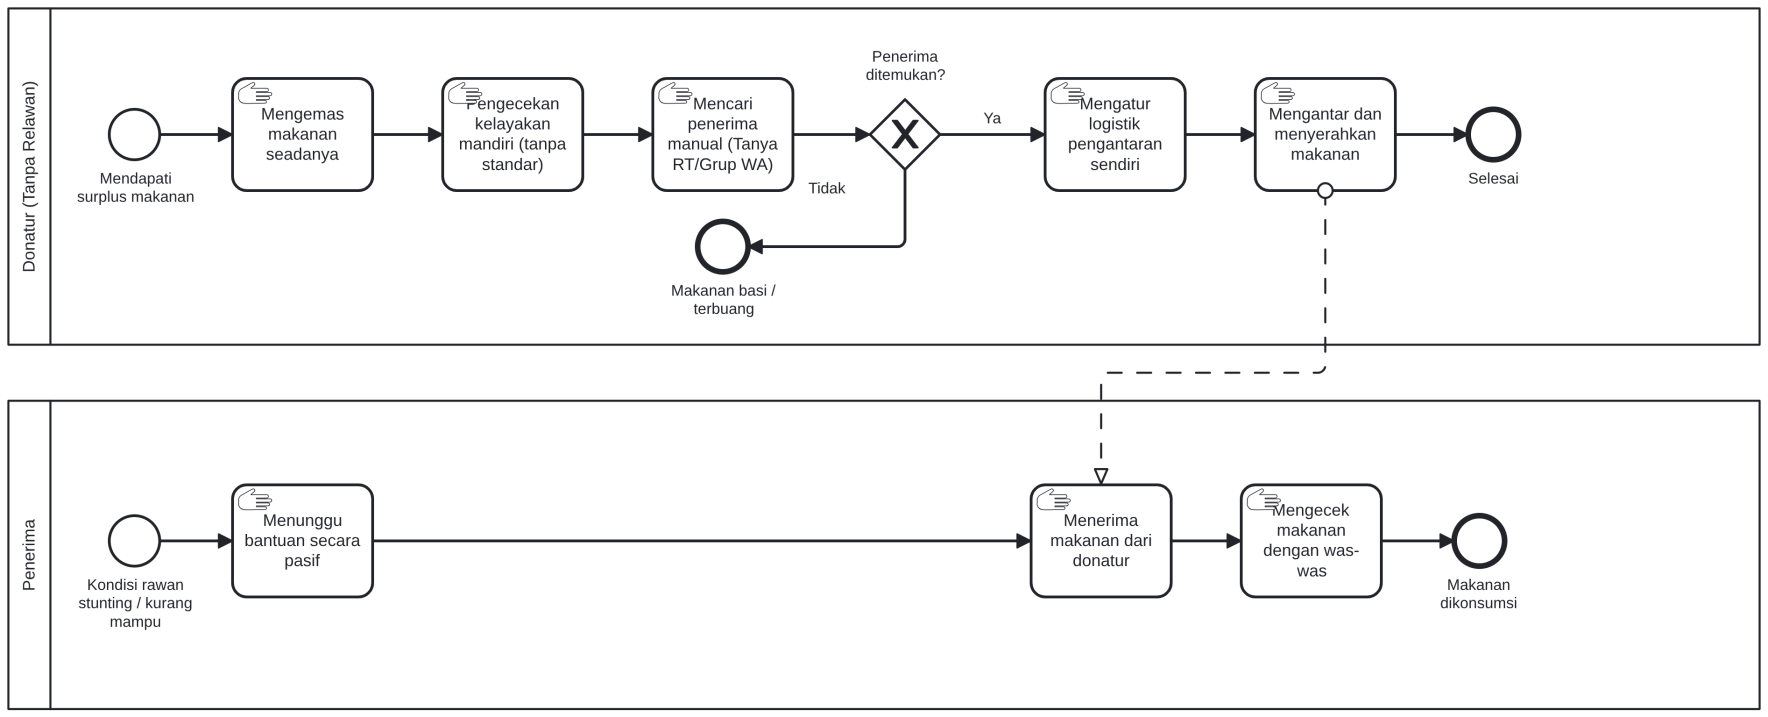
\includegraphics[width=1\linewidth]{image/bab2/as-is.png}
    \captionof{figure}{Proses Bisnis Sistem Saat Ini (BPMN As-Is)}
    \label{fig:bpmnAsIs}
    \vfill
\end{landscape}

\newpage

% Berikut adalah penjelasan detail mengenai diagram BPMN As-Is yang Diperluas (\textit{Expanded As-Is}) berdasarkan gambar tersebut.

Diagram ini membongkar realita di lapangan mengenai bagaimana proses donasi makanan sisa berjalan secara konvensional sebelum adanya intervensi sistem atau aplikasi digital. Seluruh aktivitas menggunakan \textit{Manual Task} (ikon tangan), yang menegaskan bahwa proses ini serba manual, memakan waktu, dan tidak terstandarisasi.

\subsubsection{Pool Donatur (Beban Tersentralisasi Tanpa Relawan)}
Pada sistem lama ini, Donatur memikul hampir 100\% beban operasional. Alur kerjanya adalah sebagai berikut:
\begin{itemize}
    \item Pemicu (\textit{Start Event}): Proses bermula saat donatur mendapati adanya surplus makanan (makanan berlebih yang masih layak).
    \item Persiapan Tanpa Standar: Donatur melakukan tugas "Mengemas makanan seadanya" dan "Pengecekan kelayakan mandiri (tanpa standar)". Ini adalah titik lemah pertama. Tidak ada SOP mengenai kebersihan wadah atau batas kelayakan konsumsi, murni hanya mengandalkan insting donatur.
    \item Titik Buta Informasi (\textit{Blind Spot}): Donatur kemudian "Mencari penerima manual". Aktivitas ini sangat merepotkan karena donatur harus bertanya dari mulut ke mulut (misal: ke RT setempat) atau melempar pesan di Grup WA keluarga/komunitas.
    \item Percabangan Kritis (Penerima ditemukan?):
    \begin{itemize}
        \item Jalur Gagal (Tidak): Jika pencarian memakan waktu terlalu lama atau tidak ada yang merespons, alur berbelok ke bawah menuju \textit{End Event} "Makanan basi / terbuang". Ini merepresentasikan masalah \textit{food waste} yang sering terjadi karena keterlambatan distribusi.
        \item Jalur Sukses (Ya): Jika penerima ditemukan, beban donatur belum selesai.
    \end{itemize}
    \item Kendala Logistik: Donatur harus "Mengatur logistik pengantaran sendiri". Karena ketiadaan relawan/kurir, donatur harus meluangkan waktu, tenaga, dan bensin untuk mengantar makanan tersebut.
    \item Penyelesaian: Proses diakhiri dengan "Mengantar dan menyerahkan makanan" secara langsung ke lokasi penerima.
\end{itemize}

\subsubsection{Pool Penerima (Kondisi Pasif dan Ketidakpastian)}
Di sisi seberang, alur penerima sangat pasif dan dipenuhi ketidakpastian:
\begin{itemize}
    \item Kondisi Awal: Proses penerima dipicu oleh keadaan, yaitu "Kondisi rawan stunting / kurang mampu".
    \item Sikap Pasif: Penerima hanya bisa "Menunggu bantuan secara pasif". Mereka tidak memiliki alat atau \textit{platform} untuk menyuarakan kebutuhan mereka kepada para calon donatur.
    \item Interaksi Serah Terima: Jika ada donatur yang datang, barulah penerima "Menerima makanan dari donatur" (dihubungkan oleh garis putus-putus dari \textit{pool} donatur yang merepresentasikan serah terima fisik).
    \item Isu Keamanan Pangan (\textit{Food Safety}): Setelah menerima, muncul tahap psikologis yang digambarkan sebagai "Mengecek makanan dengan was-was". Karena tidak ada jaminan atau pihak ketiga yang memvalidasi kualitas makanan tersebut, penerima mungkin merasa ragu apakah makanan tersebut masih aman dan higienis untuk dikonsumsi.
    \item Akhir Proses: Proses selesai ketika makanan akhirnya dikonsumsi.
\end{itemize}

\subsubsection{Kesimpulan Masalah (\textit{Pain Points}) pada Sistem As-Is}
Diagram ini dengan sangat jelas memetakan tiga masalah utama yang mendasari perlunya pembuatan aplikasi:
\begin{enumerate}
    \item Risiko \textit{Food Waste} yang Tinggi: Garis percabangan yang berujung pada "Makanan basi/terbuang" menunjukkan betapa rapuhnya sistem distribusi manual.
    \item Ketiadaan Dukungan Logistik: Donatur sering kali enggan mendonasikan makanannya karena malas atau tidak punya waktu untuk "Mengatur logistik pengantaran sendiri".
    \item Krisis Kepercayaan (\textit{Trust Issue}): Proses pengecekan kelayakan yang serba mandiri oleh donatur menimbulkan rasa "was-was" bagi penerima, membuktikan perlunya standarisasi dan validasi sistem (seperti pemindaian QR Code pada sistem \textit{To-Be}).
\end{enumerate}

\newpage

\begin{landscape}
    \centering
    \vfill
    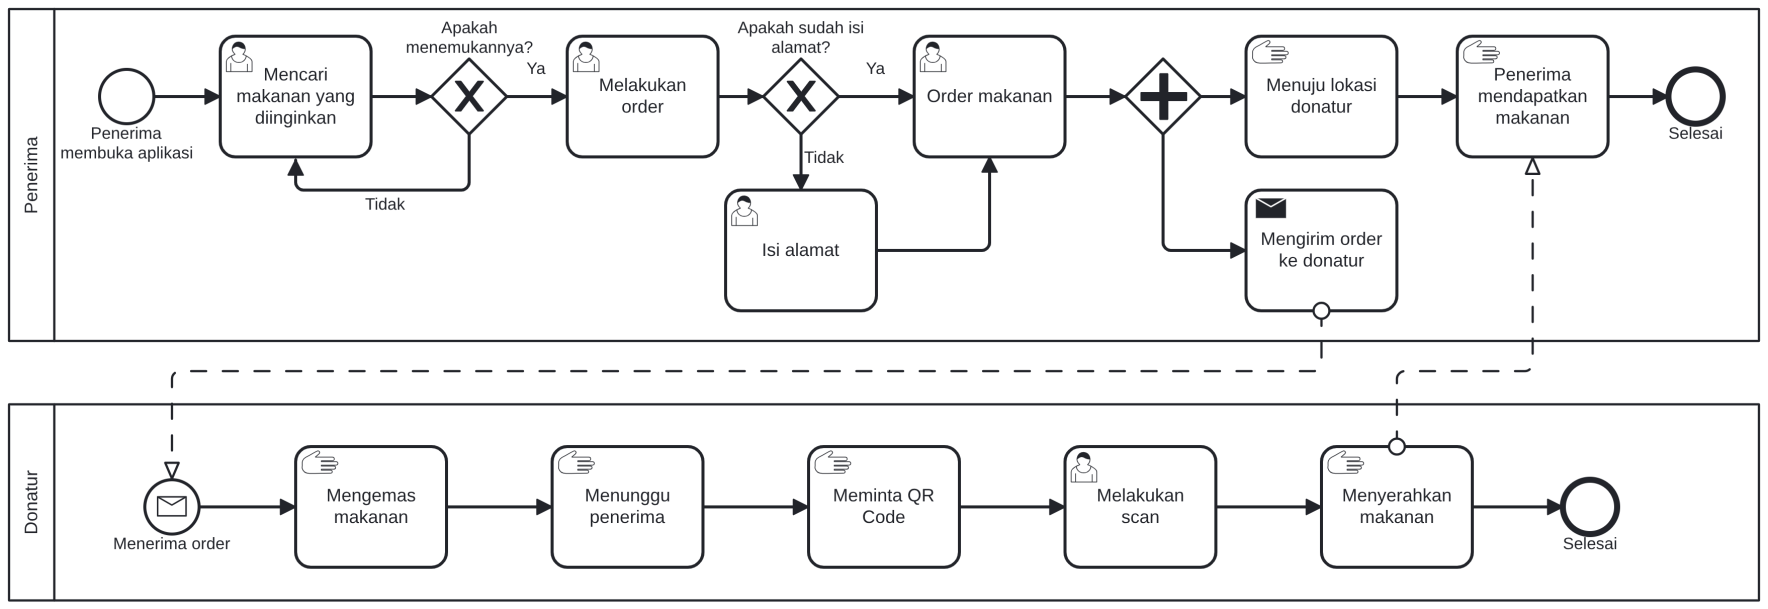
\includegraphics[width=1\linewidth]{image/bab2/to-be metode pickup.png}
    \captionof{figure}{Proses Bisnis Sistem Usulan - Metode Pickup (BPMN To-Be)}
    \label{fig:bpmnToBePickup}
    \vfill
\end{landscape}

\newpage

\subsubsection{Pool Penerima (Pusat Pemesanan dan Eksekusi Pengambilan)}
Pada metode \textit{pick-up}, aplikasi memberikan kendali penuh kepada penerima untuk bersikap proaktif. Alur detailnya adalah:
\begin{itemize}
    \item Eksplorasi dan Pemesanan Terpusat: Penerima tidak lagi hanya "menunggu bola" seperti pada sistem manual. Mereka membuka aplikasi dan langsung disajikan katalog \textit{real-time} di halaman beranda yang berisi daftar ketersediaan makanan surplus di sekitar mereka. Jika menemukan yang cocok, mereka langsung melakukan order (\textit{checkout}).
    \item Verifikasi Profil (Kelengkapan Alamat): Walaupun penerima akan mengambil sendiri, sistem tetap melakukan pengecekan (\textit{gateway}) apakah profil/alamat penerima sudah lengkap. Ini penting sebagai bentuk KYC (\textit{Know Your Customer}) untuk pendataan sistem agar \textit{user} yang bertransaksi adalah akun yang valid.
    \item Mobilisasi Mandiri: Setelah order diproses dan notifikasi terkirim ke donatur, penerima mengambil alih beban logistik. Mereka mengikuti petunjuk lokasi yang tertera di aplikasi dan bergerak secara mandiri menuju titik lokasi donatur tanpa memerlukan perantara kurir/relawan.
\end{itemize}

\subsubsection{Pool Donatur (Penyedia Donasi yang Difasilitasi)}
Sistem ini sangat meringankan beban operasional donatur. Alurnya menjadi pasif namun jauh lebih efisien:
\begin{itemize}
    \item Respons Berbasis Notifikasi (Trigger System): Donatur tidak perlu mencari siapa yang mau menerima makanannya. Sistem yang akan mencarikan. Begitu ada penerima yang melakukan order, donatur akan menerima \textit{push notification}. Notifikasi inilah yang memicu donatur untuk mulai mengemas makanan dengan layak.
    \item Menunggu Secara Pasif (Efisiensi Tenaga): Setelah mengemas, donatur cukup menunggu di tempat (rumah atau toko). Mereka bisa melanjutkan aktivitas harian mereka tanpa perlu pusing memikirkan cara mengantarkan makanan tersebut.
    \item Sistem Validasi Silang (Pemindaian QR Code): Ini adalah titik \textit{checkpoint} paling krusial dalam interaksi tatap muka. Saat penerima tiba dan mengaku sebagai pemesan, donatur wajib meminta QR Code (atau \textit{unique code}) yang tampil di layar aplikasi penerima. Donatur kemudian melakukan \textit{scan} menggunakan kameranya. Sistem akan mencocokkan data. Jika valid, serah terima fisik dilakukan, dan status order di dalam sistem otomatis berubah menjadi "Selesai".
\end{itemize}

\subsubsection{Solusi Signifikan yang Ditawarkan (Menjawab Pain Points)}
Perubahan alur ke arah digital dengan metode \textit{pick-up} ini memberikan dampak penyelesaian masalah yang terukur:
\begin{itemize}
    \item Menghapus Blind Spot Informasi Melalui Konsep "Marketplace": Sistem menjembatani informasi yang sebelumnya terputus. Donatur tidak perlu lagi menelepon atau bertanya di grup-grup komunitas. Ketersediaan makanan langsung terekspos kepada audiens yang tepat (penerima terdaftar), mempercepat proses \textit{matchmaking} antara makanan sisa dan pihak yang lapar.
    \item Memotong Rantai Logistik yang Menghambat: Pada sistem lama, tingginya angka \textit{food waste} sering kali terjadi karena donatur sibuk dan tidak ada yang bisa mengantarkan makanan. Dengan sistem \textit{pick-up}, tanggung jawab pergerakan logistik dialihkan kepada pihak yang memang membutuhkan makanan tersebut (penerima). Ini memastikan makanan lebih cepat diselamatkan selagi masih layak konsumsi.
    \item Peningkatan Keamanan, Validitas, dan Rekam Jejak (Traceability):
    \begin{itemize}
        \item Anti-Salah Sasaran: Pemindaian QR Code mengeliminasi risiko penipuan di lapangan. Donatur memiliki jaminan kepastian bahwa orang yang mengambil makanan adalah benar-benar pengguna terdaftar yang melakukan order.
        \item Digital Audit Trail: Setiap kali QR code dipindai dan makanan diserahkan, sistem mencatat waktu, lokasi, dan aktor yang terlibat ke dalam basis data. Ini menghasilkan riwayat transaksi yang transparan, memberikan rasa aman bagi kedua belah pihak.
    \end{itemize}
\end{itemize}

\newpage

\begin{landscape}
    \centering
    \vfill
    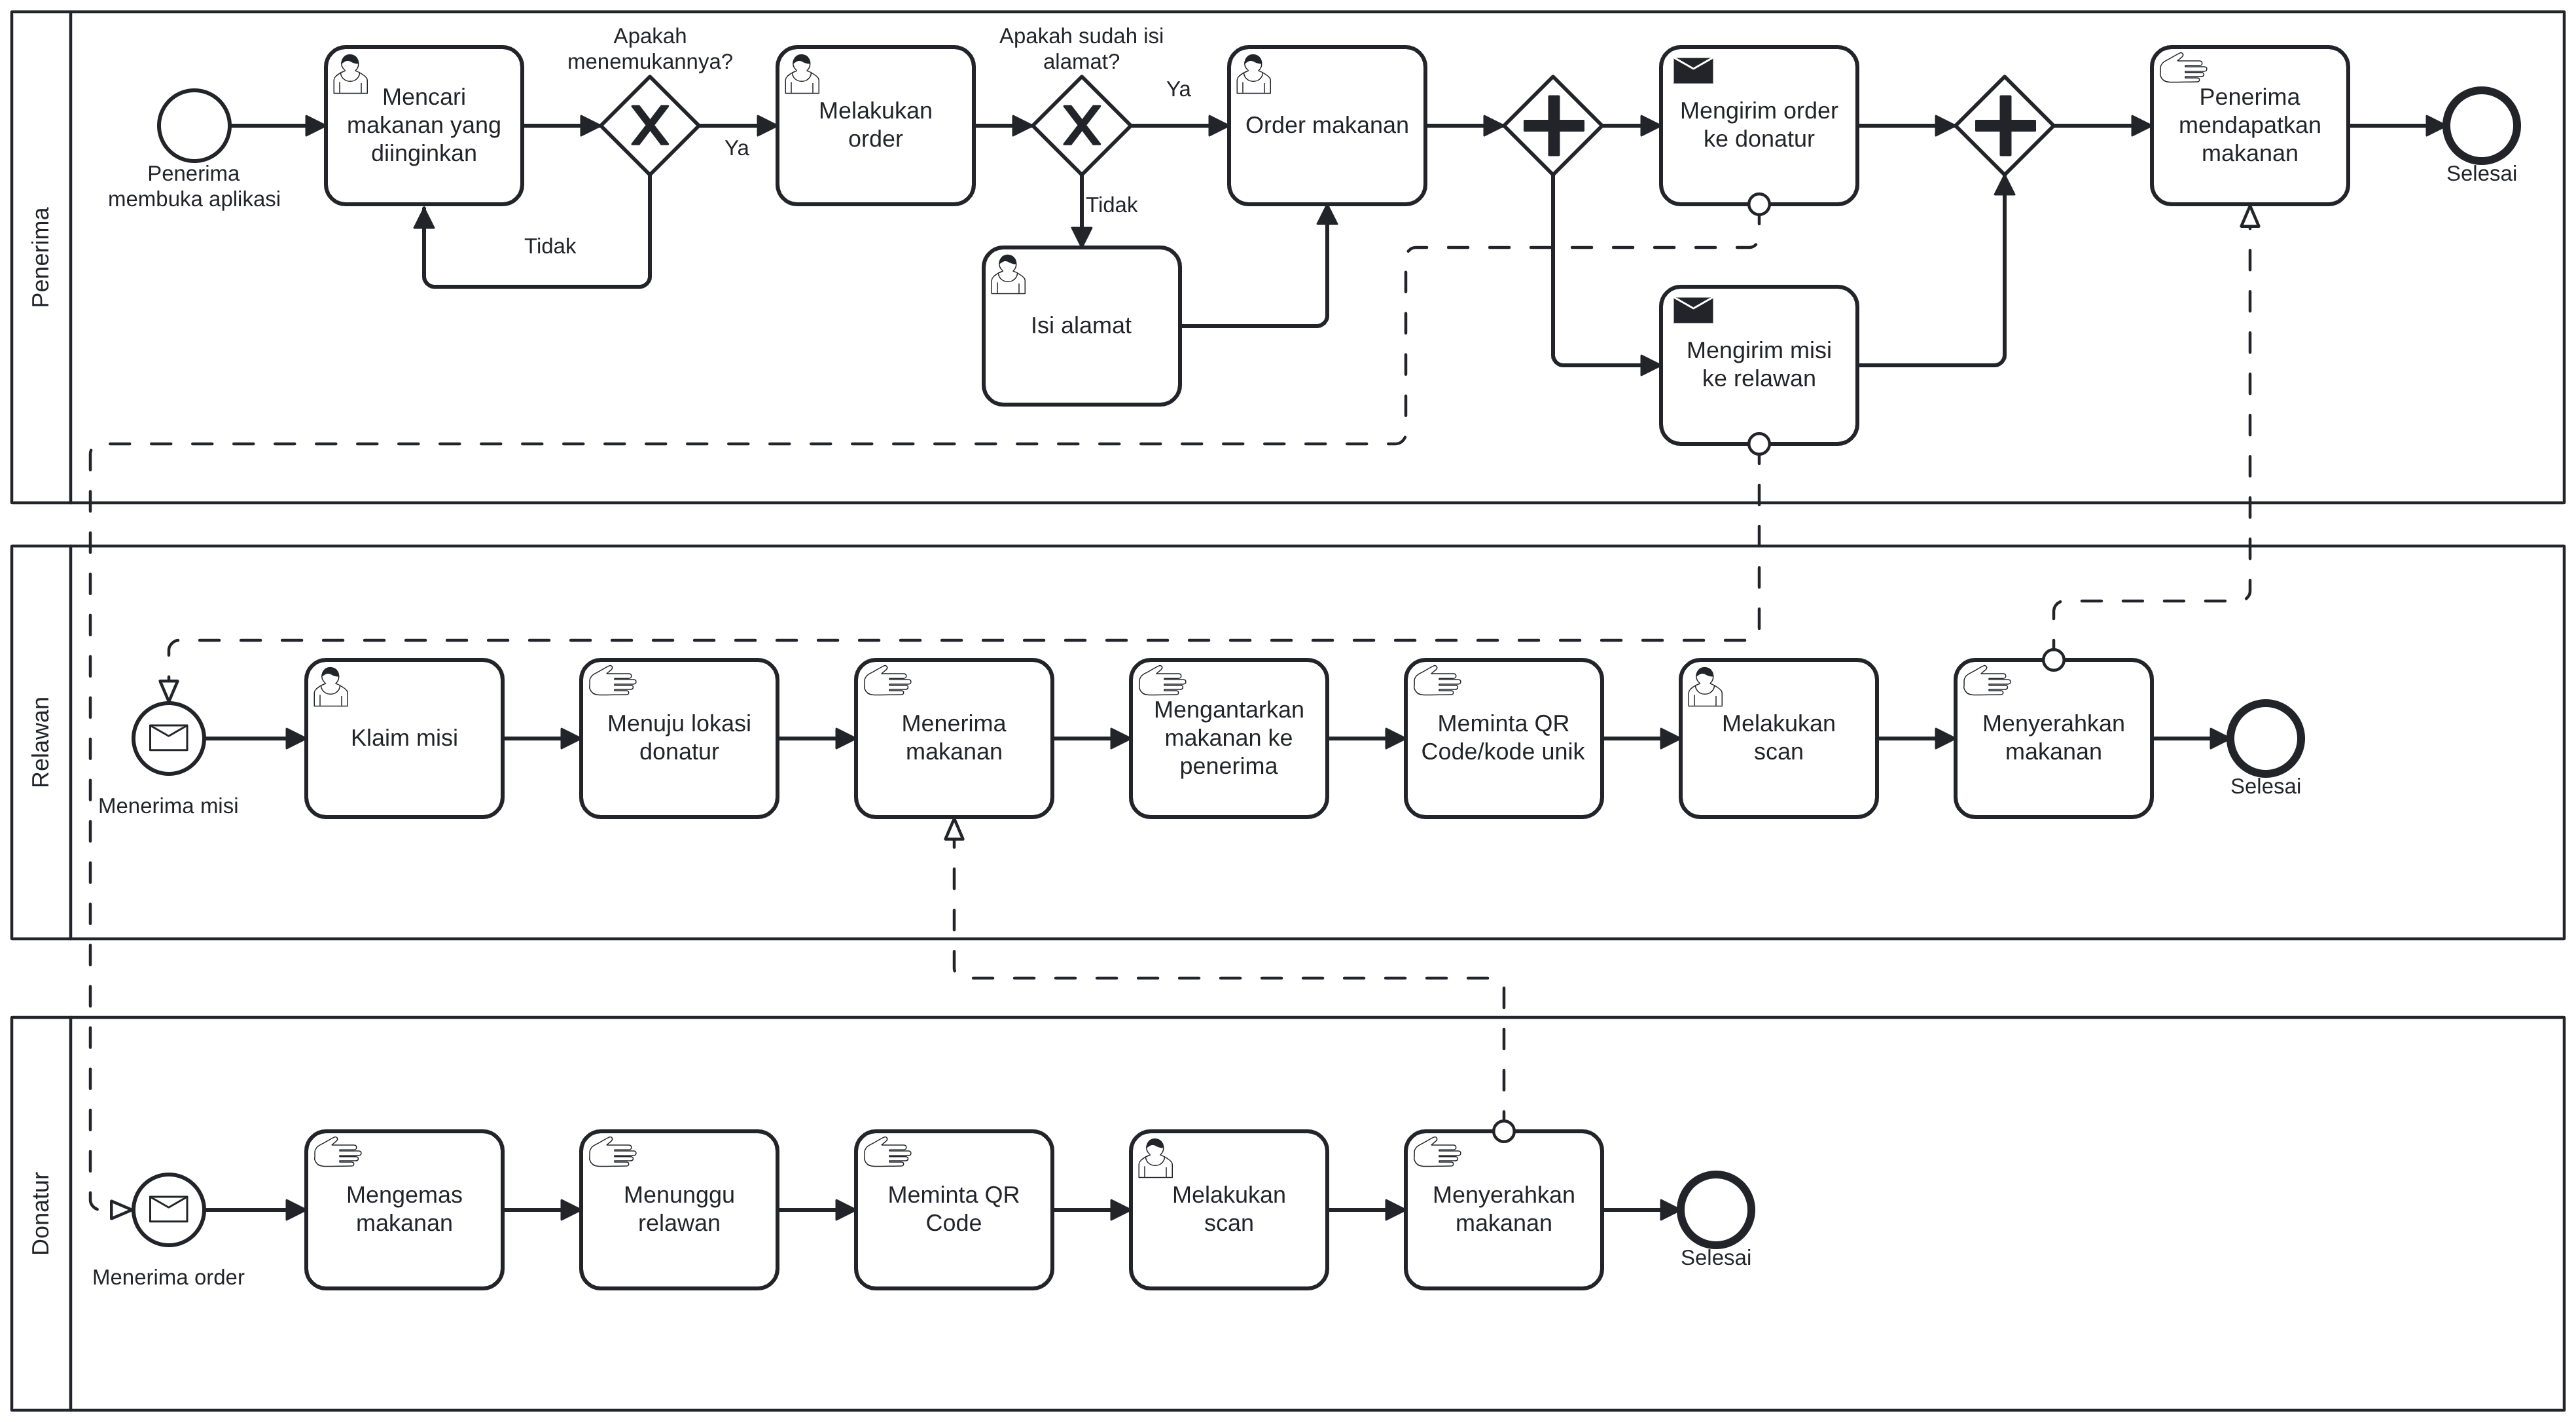
\includegraphics[width=1\linewidth]{image/bab2/to-be metode diantar.png}
    \captionof{figure}{Proses Bisnis Sistem Usulan - Metode Diantar (BPMN To-Be)}
    \label{fig:bpmnToBeDiantar}
    \vfill
\end{landscape}

\newpage

Skenario ini merupakan solusi komprehensif yang melibatkan tiga aktor sekaligus: Penerima, Donatur, dan kehadiran entitas baru yaitu Relawan. Relawan bertindak sebagai pahlawan logistik yang menjembatani donatur dan penerima.

\subsubsection{Pool Penerima (Pemesan \& Penerima Akhir)}
Pada skenario ini, penerima tetap menjadi inisiator pesanan, namun mereka hanya perlu menunggu di lokasi setelah pesanan dibuat. Alur detailnya:
\begin{itemize}
    \item Eksplorasi \& Validasi Alamat: Proses dimulai dari membuka aplikasi, mencari makanan, dan melakukan order. Sistem mengecek ketersediaan alamat; jika belum ada, pengguna wajib mengisi alamat agar relawan tahu titik pengantaran.
    \item Aksi Paralel (\textit{Parallel Gateway}): Ini adalah titik krusial (ditandai dengan ikon +). Setelah tombol "Order makanan" ditekan, sistem melakukan dua aksi pengiriman pesan (\textit{Send Task}) secara bersamaan:
    \begin{enumerate}
        \item Mengirimkan notifikasi "Order" kepada Donatur agar makanan disiapkan.
        \item Mem-\textit{broadcast} pesanan tersebut sebagai "Misi" kepada para Relawan di sekitar lokasi.
    \end{enumerate}
    \item Menunggu Kedatangan: Penerima kemudian menunggu di lokasi hingga relawan tiba untuk menyerahkan makanan. Proses selesai ketika makanan sudah di tangan penerima ("Penerima mendapatkan makanan").
\end{itemize}

\subsubsection{Pool Donatur (Penyedia Donasi)}
Alur donatur pada metode antar sangat mirip dengan metode \textit{pick-up}, namun lawan interaksinya berbeda:
\begin{itemize}
    \item Persiapan: Donatur menerima notifikasi order, lalu mulai mengemas makanan tersebut.
    \item Menunggu Relawan: Alih-alih menunggu penerima, donatur kini bersiap menunggu kedatangan Relawan yang telah mengklaim misi tersebut.
    \item Verifikasi Tahap 1 (QR Code): Ketika relawan tiba, donatur akan meminta QR Code dari relawan. Donatur kemudian melakukan \textit{scan} via aplikasi. Hal ini memastikan bahwa makanan diserahkan kepada relawan yang sah dan terdaftar di sistem, bukan sembarang orang.
    \item Serah Terima Tahap 1: Setelah validasi berhasil, donatur menyerahkan makanan kepada relawan. Proses bagi donatur pun selesai.
\end{itemize}

\subsubsection{Pool Relawan (Pahlawan Logistik)}
Ini adalah alur operasional utama bagi aktor ketiga yang bertugas menyelesaikan kendala logistik:
\begin{itemize}
    \item Penerimaan \& Klaim Misi: Relawan menerima notifikasi misi (berasal dari \textit{broadcast} sistem penerima). Jika bersedia, relawan menekan tombol "Klaim misi" di aplikasi.
    \item Fase Pengambilan (\textit{Pick-up} dari Donatur): Relawan bergerak menuju lokasi donatur. Sesampainya di sana, mereka menjalani proses verifikasi QR dari donatur, lalu "Menerima makanan".
    \item Fase Pengantaran (\textit{Delivery} ke Penerima): Relawan kemudian membawa makanan tersebut dan bergerak ("Mengantarkan makanan") menuju alamat penerima yang tertera di sistem.
    \item Verifikasi Tahap 2 (QR Code): Setibanya di lokasi tujuan, relawan tidak langsung memberikan makanan. Relawan bertugas "Meminta QR Code/kode unik" dari penerima, lalu "Melakukan scan" menggunakan aplikasinya.
    \item Serah Terima Akhir: Setelah sistem menyatakan data penerima valid, relawan menyerahkan makanan kepada penerima. Misi logistik pun selesai.
\end{itemize}

\subsubsection{Interaksi Lintas Aktor (\textit{Message Flow} - Garis Putus-putus)}
Diagram ini menunjukkan pertukaran informasi dan barang yang sangat terstruktur:
\begin{enumerate}
    \item Penerima $\rightarrow$ Donatur: Sistem mengirimkan detail order untuk disiapkan.
    \item Penerima $\rightarrow$ Relawan: Sistem menembakkan order tersebut ke \textit{pool} misi relawan.
    \item Donatur $\rightarrow$ Relawan: Interaksi fisik di mana Donatur menyerahkan kotak makanan kepada Relawan (setelah lolos \textit{scan} QR).
    \item Relawan $\rightarrow$ Penerima: Interaksi fisik akhir di mana Relawan menyerahkan kotak makanan kepada Penerima (juga setelah lolos \textit{scan} QR).
\end{enumerate}

\subsubsection{Solusi Signifikan (Perbaikan dari As-Is)}
\begin{itemize}
    \item Penyelesaian \textit{Bottleneck} Logistik: Kelemahan utama sistem lama, di mana makanan membusuk karena donatur tidak bisa mengantar dan penerima tidak bisa mengambil, terpecahkan oleh kehadiran Relawan.
    \item Keamanan Berlapis (\textit{Double-Blind Verification}): Sistem ini menerapkan keamanan ekstra ketat. Makanan melewati dua kali proses pemindaian QR Code: \textit{Donatur-ke-Relawan} dan \textit{Relawan-ke-Penerima}. Ini menjamin rantai pasok (\textit{chain of custody}) makanan tercatat sempurna di \textit{database} dari hulu ke hilir.
\end{itemize}

\newpage

\subsection{Pengalaman Pengguna}
Guna memastikan bahwa platform Food AI Rescue yang dikembangkan dapat menyelesaikan permasalahan secara akurat dan tepat sasaran, penelitian ini menerapkan pendekatan desain berpusat pada manusia (\textit{Human-Centered Design}). Pendekatan ini secara spesifik memetakan pengalaman dari target pengguna utama di lapangan, yakni pihak donatur, penerima donasi, dan relawan logistik, ketika mereka masih melakukan proses penyaluran surplus makanan secara manual atau konvensional (\textit{As-Is}). Hasil pemetaan permasalahan tersebut kemudian dituangkan ke dalam tiga artefak \textit{User Experience} (UX), meliputi \textit{User Persona}, \textit{Empathy Map}, dan \textit{User Journey Map}, yang dijabarkan sebagai berikut:

\begin{figure}[H]
    \centering
    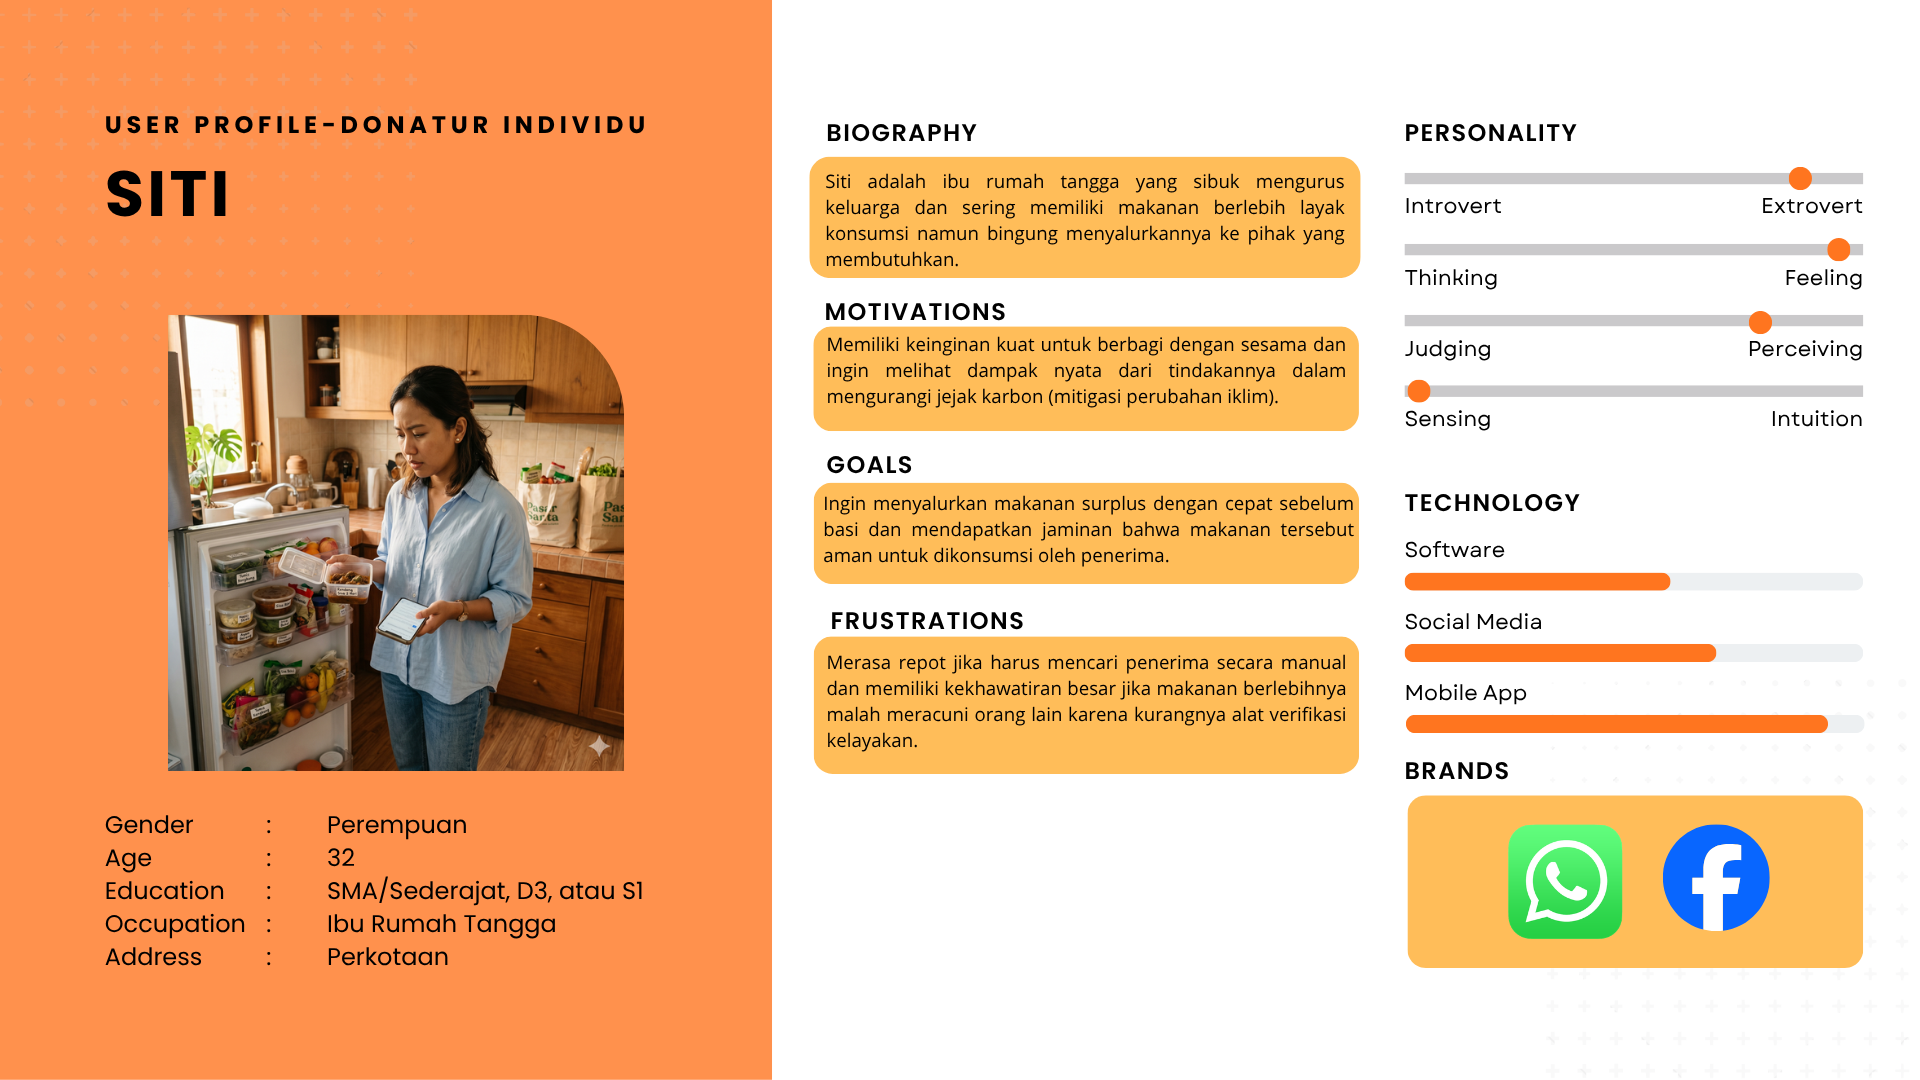
\includegraphics[width=1\textwidth]{image/bab2/segmentasi/UserPersona/Salinan dari baso arif/UP_DONATUR INDIVIDU.png}
    \caption{User Persona Donatur Individu}
    \label{fig:userPersonaDonaturIndividu}
\end{figure}

Penjelasan Profil (Siti):
Siti (32 tahun) merupakan seorang ibu rumah tangga di area perkotaan dengan jadwal padat. Ia kerap mendapati sisa bahan makanan layak konsumsi di dapur, namun kebingungan mencari cara aman untuk menyalurkannya.
\begin{itemize}
    \item Motivasi: Tergerak untuk berbagi dengan sesama dan ingin melihat dampak langsung dari usahanya dalam menekan jejak emisi karbon (mitigasi perubahan iklim).
    \item Tujuan: Mampu mendistribusikan makanan surplus dengan cepat sebelum membusuk, sekaligus memperoleh kepastian bahwa makanan tersebut higienis dan aman dikonsumsi oleh penerima.
    \item Frustrasi: Merasa sangat repot apabila harus mencari target penerima donasi secara mandiri. Terdapat kekhawatiran besar bahwa makanan berlebihnya justru dapat meracuni orang lain karena ketiadaan alat verifikasi kelayakan.
    \item Preferensi: Aplikasi \textit{mobile}, perangkat lunak (\textit{software}), media sosial, serta nilai efisiensi dalam kepedulian sosial.
\end{itemize}

% \newpage

\begin{figure}[H]
    \centering
    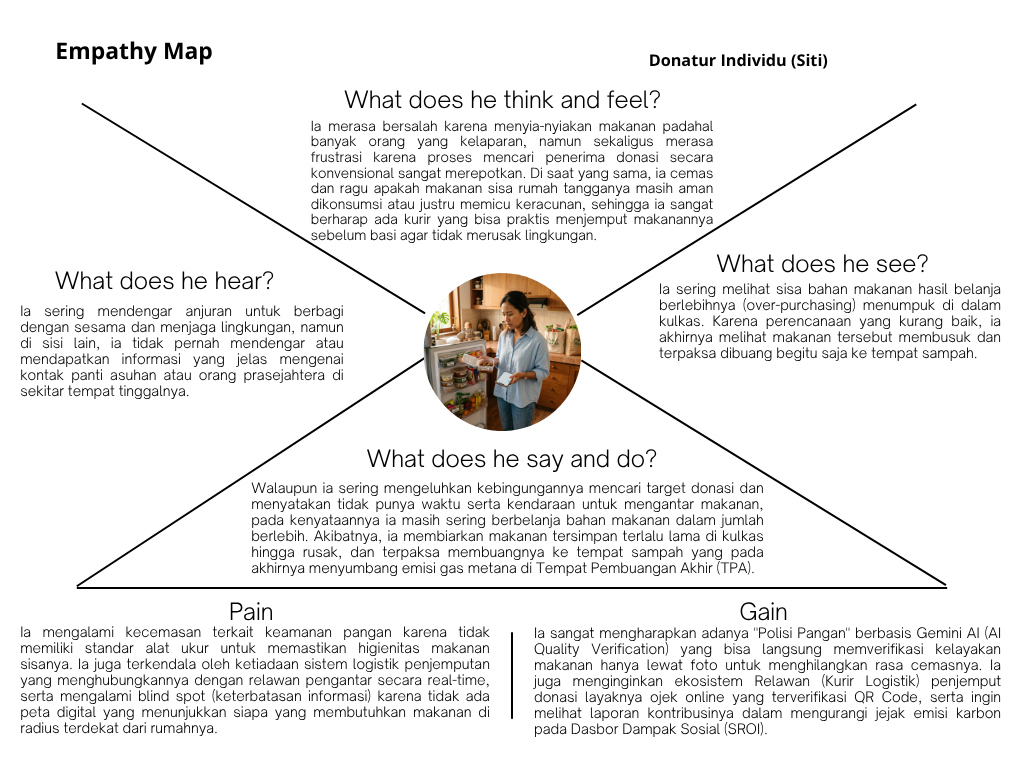
\includegraphics[width=1\textwidth]{image/bab2/segmentasi/EmpathyMap/Black and White Simple Empathy Map Brainstorm/EM_DONATUR_INDIVIDU.png}
    \caption{Empathy Map Donatur Individu}
    \label{fig:empathyMapDonaturIndividu}
\end{figure}


Penjelasan Aspek Empathy Map (Siti):
Siti adalah representasi donatur skala rumah tangga yang sering memiliki makanan berlebih, berniat kuat untuk menyumbang, namun terhalang oleh keraguan dan minimnya akses.
\begin{itemize}
    \item THINKS \& FEELS: Merasa bersalah karena menyia-nyiakan makanan di saat banyak orang kelaparan, namun sekaligus frustrasi akibat proses pencarian penerima yang merepotkan. Ia cemas apakah sisa makanannya masih aman dimakan atau justru memicu keracunan, sehingga sangat berharap ada layanan kurir penjemputan praktis sebelum makanannya membusuk dan merusak lingkungan.
    \item HEARS: Kerap mendengar anjuran untuk saling berbagi dan menjaga lingkungan, tetapi di sisi lain, ia tidak pernah mendapatkan informasi pasti atau kontak mengenai panti asuhan maupun warga prasejahtera di sekitar tempat tinggalnya.
    \item SEES: Menyaksikan langsung tumpukan sisa bahan makanan di kulkas akibat kebiasaan belanja berlebih (\textit{over-purchasing}). Karena minimnya perencanaan, ia akhirnya hanya bisa melihat makanan tersebut membusuk dan terpaksa membuangnya ke tempat sampah.
    \item SAYS \& DOES: Meskipun sering mengeluh kebingungan mencari target donasi dan menyatakan tidak punya waktu serta kendaraan untuk mengantar, pada praktiknya ia tetap membiarkan makanan tersimpan terlalu lama di kulkas. Akibatnya, makanan tersebut rusak dan dibuang ke TPA, yang pada akhirnya menyumbang emisi gas metana.
    \item PAINS: Mengalami kecemasan terkait keamanan pangan karena ketiadaan alat ukur higienitas. Ia juga terhambat oleh ketiadaan sistem logistik penjemputan (\textit{pick-up}) \textit{real-time}, serta mengalami \textit{blind spot} (keterbatasan informasi) mengenai lokasi pihak yang membutuhkan di radius terdekatnya.
    \item GAINS: Sangat mendambakan kehadiran "Polisi Pangan" berbasis AI yang mampu memvalidasi kelayakan makanan hanya melalui foto. Ia juga menginginkan ekosistem Relawan Kurir layaknya ojek \textit{online} yang terverifikasi QR Code, serta Dasbor SROI untuk melihat laporan kontribusinya dalam mengurangi jejak karbon.
\end{itemize}

% \newpage

\begin{figure}[H]
    \centering
    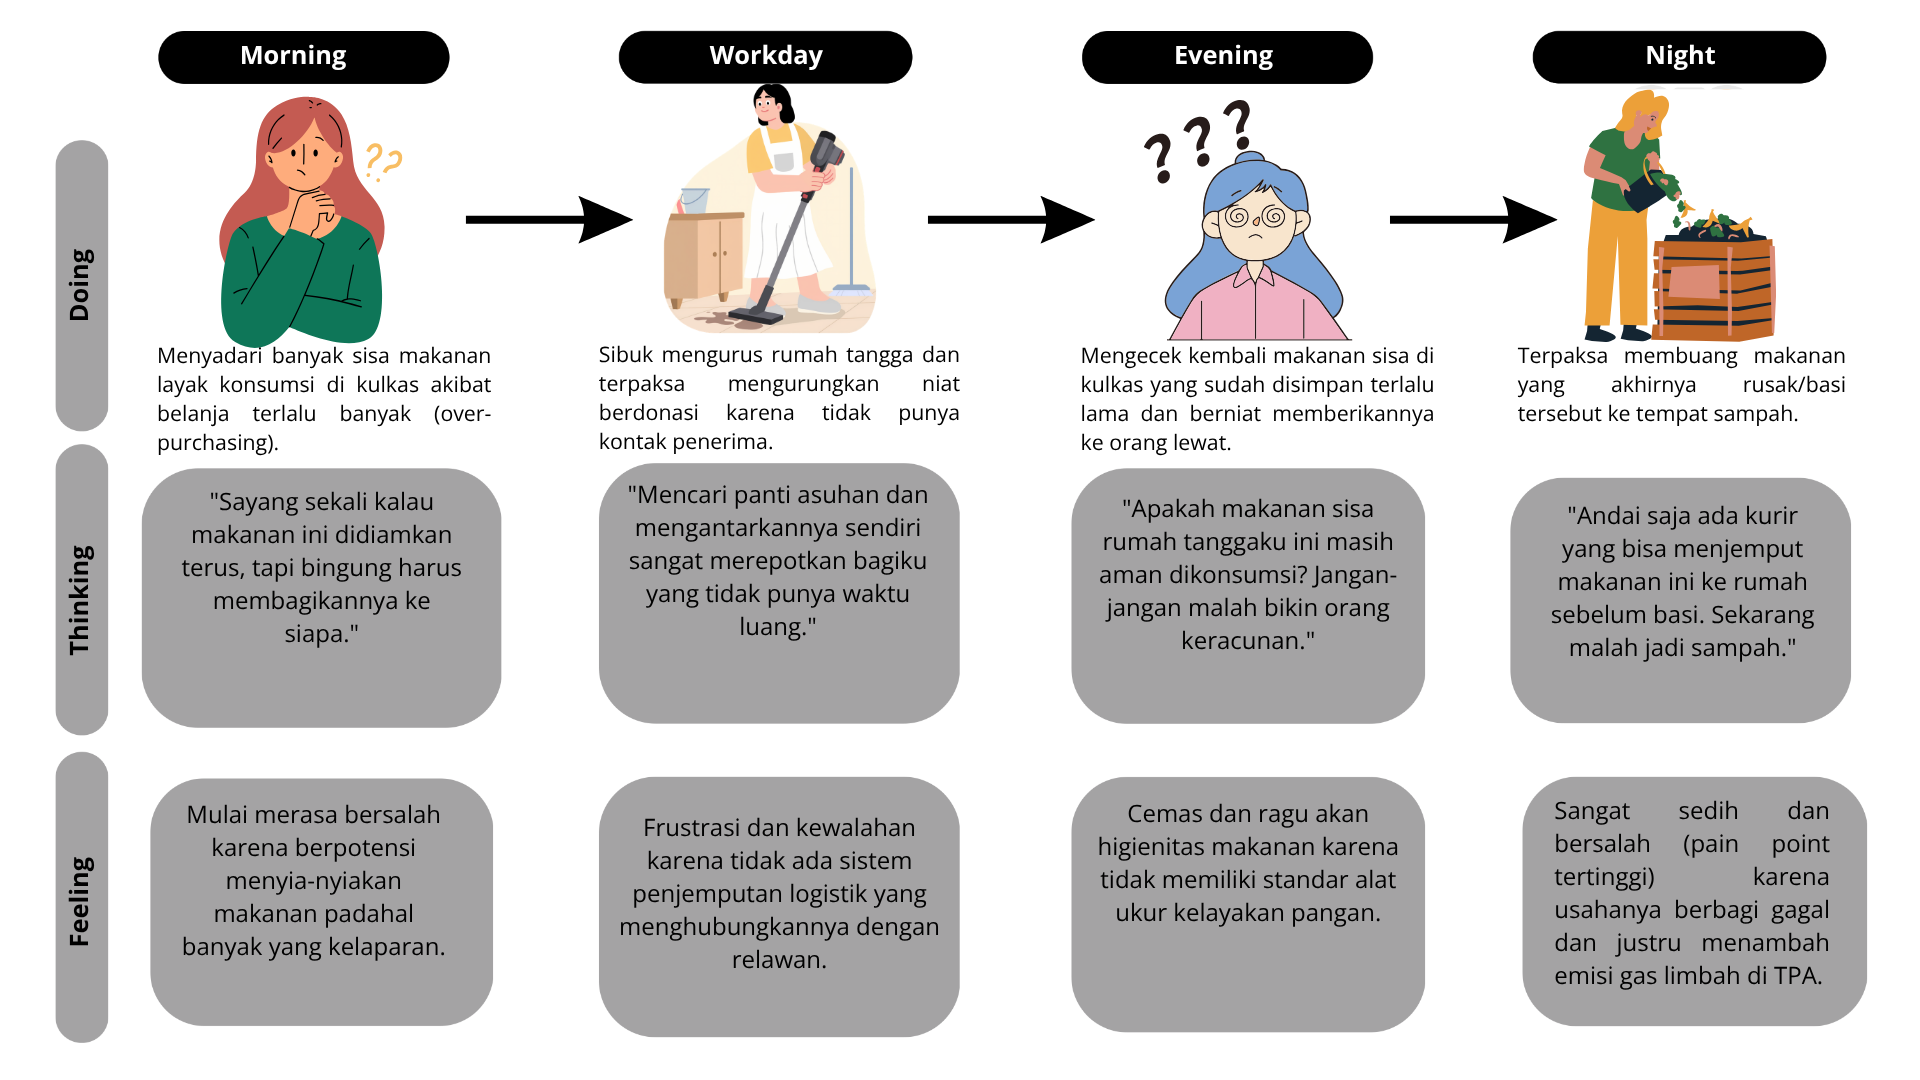
\includegraphics[width=0.99\textwidth]{image/bab2/segmentasi/CustomerJourneyMap/Salinan dari Template Journey Map/CJM_DONATUR_INDIVIDU.png}
    \caption{Customer Journey Map Donatur Individu}
    \label{fig:customerJourneyMapDonaturIndividu}
\end{figure}

Penjelasan Fase Customer Journey Map (Siti): \\
\textit{Fase perjalanan: Penumpukan Makanan $\rightarrow$ Keterbatasan Akses $\rightarrow$ Krisis Kepercayaan $\rightarrow$ Pembuangan \& Penyesalan}
\begin{description}
    \item[Penumpukan Makanan (Pagi):] Siti menyadari adanya banyak sisa makanan yang masih layak konsumsi di dalam kulkas akibat belanja berlebihan. Ia mulai didera rasa bersalah karena berpotensi menyia-nyiakan makanan tersebut, namun kebingungan harus menyalurkannya ke mana. Peluang Solusi (FAR): Fitur rekomendasi resep masakan berbasis AI untuk memanfaatkan bahan sisa.
    \item[Keterbatasan Akses (Siang):] Di tengah kesibukannya mengurus rumah tangga, Siti terpaksa mengurungkan niat untuk berdonasi karena ia tidak memiliki kontak penerima dan merasa sangat merepotkan jika harus mencari sekaligus mengantarkannya sendiri tanpa waktu luang. Peluang Solusi (FAR): Sistem panggilan Relawan Kurir secara instan untuk penjemputan langsung ke rumah.
    \item[Krisis Kepercayaan (Sore):] Ia kembali mengecek makanan tersebut dan berniat membagikannya ke orang lewat, namun tiba-tiba merasa cemas dan ragu. Tanpa adanya standar alat ukur, ia takut makanannya sudah tidak higienis dan malah menyebabkan keracunan. Peluang Solusi (FAR): Verifikasi AI \textit{Quality Verification} ("Polisi Pangan") untuk memastikan keamanan pangan secara instan.
    \item[Pembuangan \& Penyesalan (Malam):] Pada akhirnya, Siti terpaksa membuang makanan yang sudah terlanjur basi tersebut ke tempat sampah. Ia merasa sangat sedih dan bersalah (\textit{Pain Point Tertinggi}) karena usahanya untuk berbagi berujung gagal, dan ia justru berkontribusi menambah emisi gas limbah di TPA. Peluang Solusi (FAR): Dasbor SROI Pribadi yang memotivasi pengguna dengan menampilkan total porsi terselamatkan dan emisi yang dicegah.
\end{description}

% \clearpage

\begin{figure}[H]
    \centering
    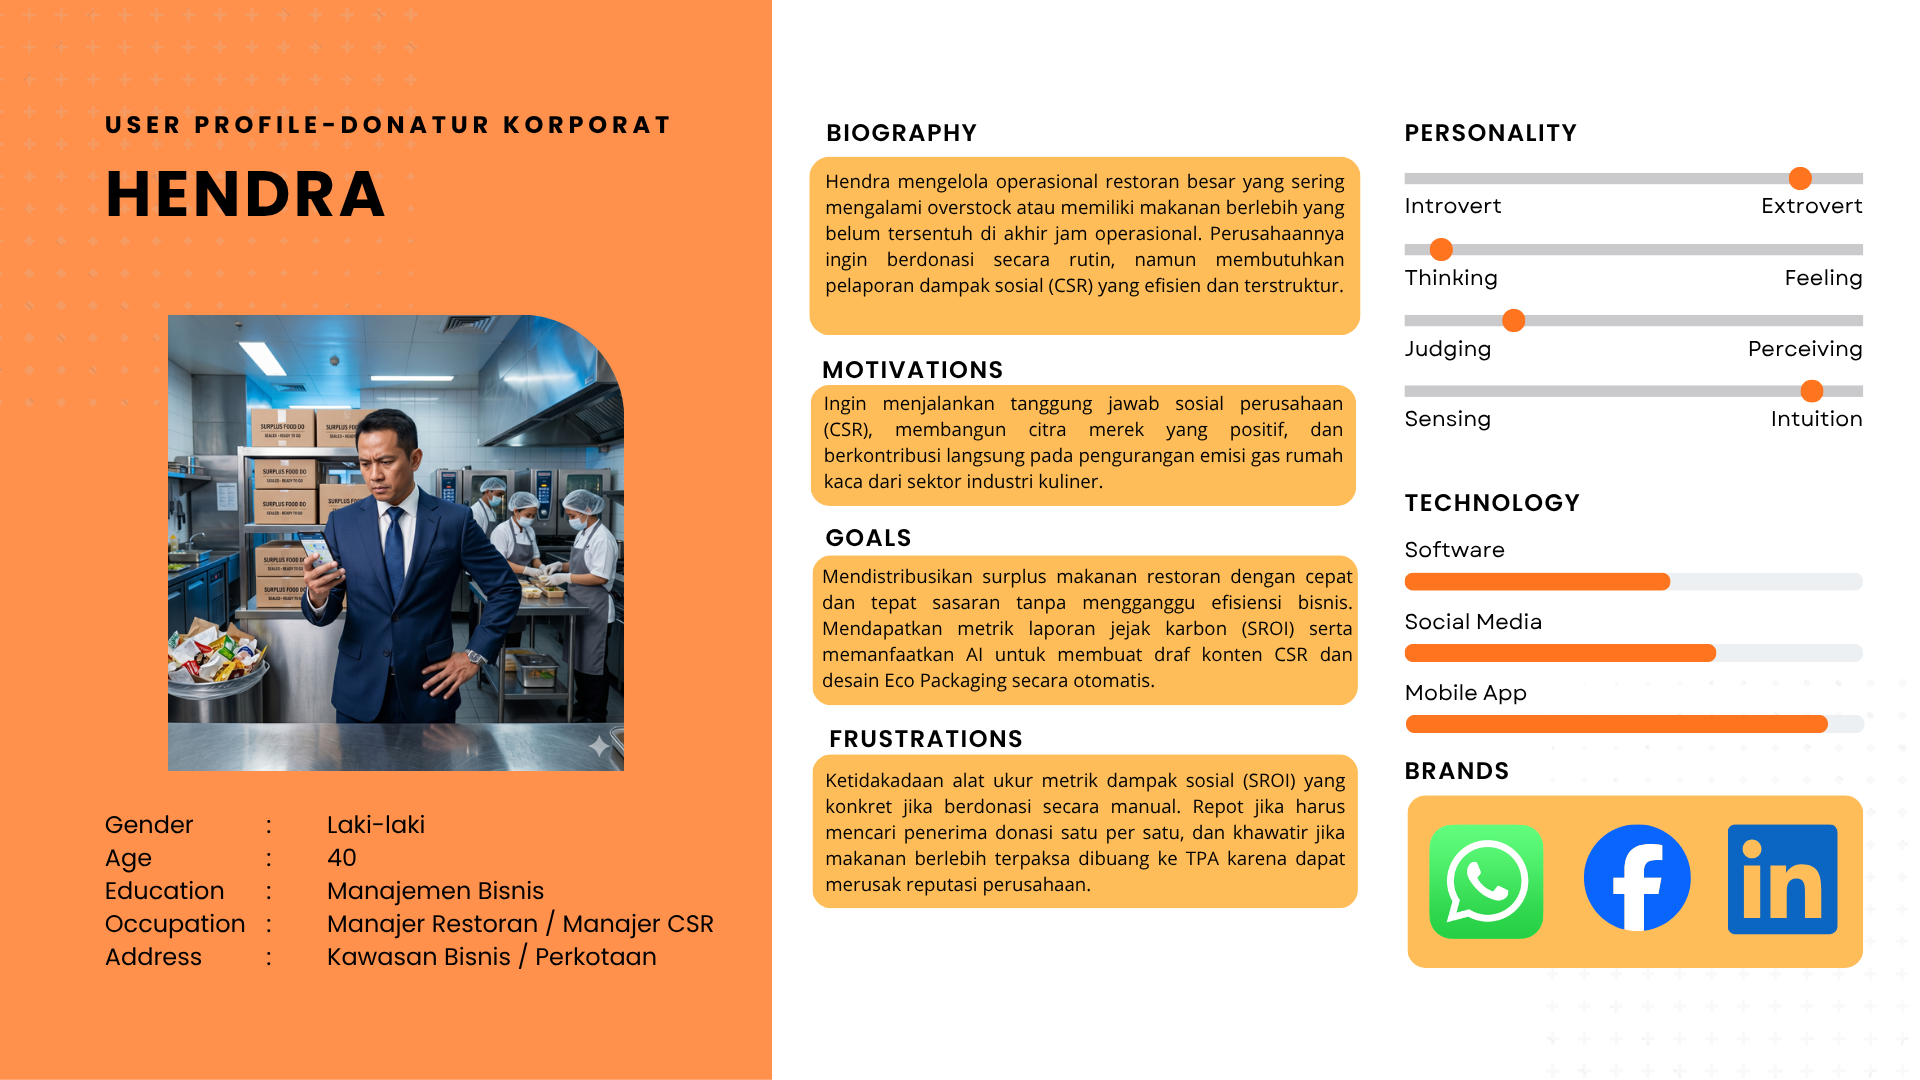
\includegraphics[width=1\textwidth]{image/bab2/segmentasi/UserPersona/Salinan dari baso arif/UP_DONATUR KORPORAT.png}
    \caption{User Persona Donatur Korporat}
    \label{fig:userPersonaDonaturKorporat}
\end{figure}

Penjelasan Profil (Hendra):
Hendra (40 tahun) menjabat sebagai manajer restoran sekaligus penanggung jawab CSR yang berhadapan dengan masalah \textit{overstock} makanan layak konsumsi di penghujung jam operasional. Perusahaannya memiliki inisiatif untuk rutin berdonasi, namun sangat membutuhkan sistem pelaporan dampak sosial yang efisien dan terstruktur.
\begin{itemize}
    \item Motivasi: Berkomitmen menjalankan kewajiban CSR perusahaan, meningkatkan citra positif merek, serta berkontribusi nyata dalam menekan emisi gas rumah kaca dari sektor industri kuliner.
    \item Tujuan: Mendistribusikan surplus makanan restoran secara cepat dan tepat sasaran tanpa mengorbankan efisiensi operasional bisnis. Ia juga ingin mendapatkan metrik Laporan Jejak Karbon (SROI) serta memanfaatkan teknologi AI untuk mengotomatisasi penyusunan konten CSR.
    \item Frustrasi: Ketidakadaan alat ukur metrik dampak sosial (SROI) yang valid saat berdonasi manual. Ia merasa repot jika harus mencari penerima satu per satu, dan sangat khawatir jika surplus makanan terpaksa dibuang ke TPA karena dapat merusak reputasi perusahaan.
    \item Preferensi: Aplikasi \textit{mobile}, perangkat lunak (\textit{software}), integrasi AI, media sosial, dan metrik bisnis yang selaras dengan kepedulian lingkungan.
\end{itemize}


\begin{figure}[H]
    \centering
    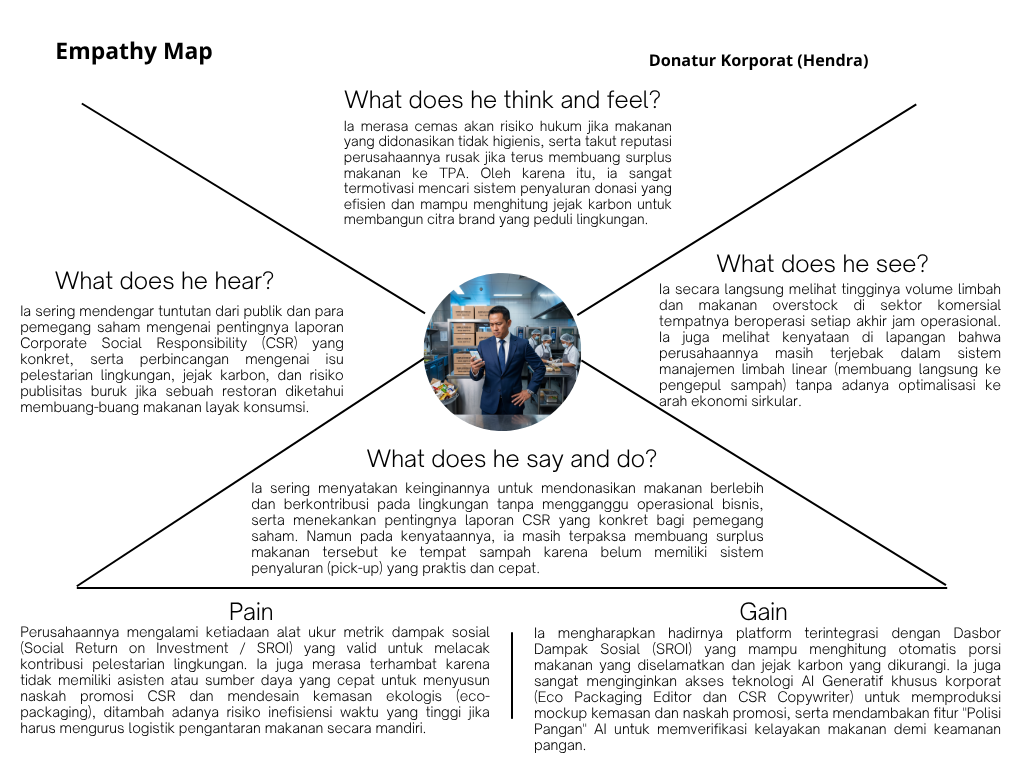
\includegraphics[width=1\textwidth]{image/bab2/segmentasi/EmpathyMap/Black and White Simple Empathy Map Brainstorm/EM_DONATUR_KORPORAT.png}
    \caption{Empathy Map Donatur Korporat}
    \label{fig:empathyMapDonaturKorporat}
\end{figure}

Penjelasan Aspek Empathy Map (Hendra):
Hendra adalah manajer restoran komersial yang ingin menyalurkan surplus makanan dengan praktis, namun sangat tertekan oleh tuntutan pelaporan reputasi dan efisiensi operasional.
\begin{itemize}
    \item THINKS \& FEELS: Dirundung kecemasan terkait potensi risiko hukum apabila makanan donasi terbukti tidak higienis. Di sisi lain, ia takut reputasi bisnisnya hancur jika terus-menerus membuang surplus ke TPA. Oleh karena itu, ia sangat termotivasi mencari sistem penyaluran efisien yang mampu menghitung jejak karbon demi citra merek peduli lingkungan.
    \item HEARS: Terus-menerus mendengar desakan dari publik dan pemegang saham mengenai urgensi pelaporan CSR yang konkret. Ia juga sering mendengar perbincangan terkait isu kelestarian lingkungan, jejak karbon, serta ancaman publisitas buruk bagi restoran yang kedapatan membuang makanan layak konsumsi.
    \item SEES: Menghadapi langsung realita tingginya volume limbah dan makanan \textit{overstock} di sektor komersial setiap kali jam operasional berakhir. Ia melihat kenyataan di lapangan bahwa perusahaannya masih terbelenggu dalam sistem manajemen limbah linear (membuang langsung ke pengepul sampah) tanpa optimalisasi ke arah ekonomi sirkular.
    \item SAYS \& DOES: Kerap mengutarakan niat mendonasikan makanan berlebih tanpa mengganggu ritme operasional bisnis, serta menekankan pentingnya laporan CSR yang nyata bagi investor. Namun pada kenyataannya, ketiadaan sistem penyaluran (\textit{pick-up}) yang cepat memaksanya untuk terus membuang surplus makanan tersebut ke tempat sampah.
    \item PAINS: Perusahaannya mengalami krisis ketiadaan alat ukur metrik dampak sosial (SROI) yang valid untuk melacak kontribusi pelestarian lingkungan. Ia juga merasa terhambat karena tidak memiliki asisten cepat untuk menyusun naskah promosi CSR dan desain kemasan ekologis, ditambah tingginya risiko inefisiensi waktu jika mengurus logistik pengantaran sendiri.
    \item GAINS: Sangat menantikan platform terintegrasi dengan Dasbor Dampak Sosial (SROI) yang mampu menghitung otomatis porsi makanan terselamatkan dan jejak karbon yang dikurangi. Ia mendambakan fitur AI Generatif khusus korporat (\textit{Eco Packaging Editor} dan \textit{CSR Copywriter}) untuk memproduksi \textit{mockup} promosi, serta "Polisi Pangan" AI untuk memvalidasi kelayakan demi keamanan pangan.
\end{itemize}

\begin{figure}[H]
    \centering
    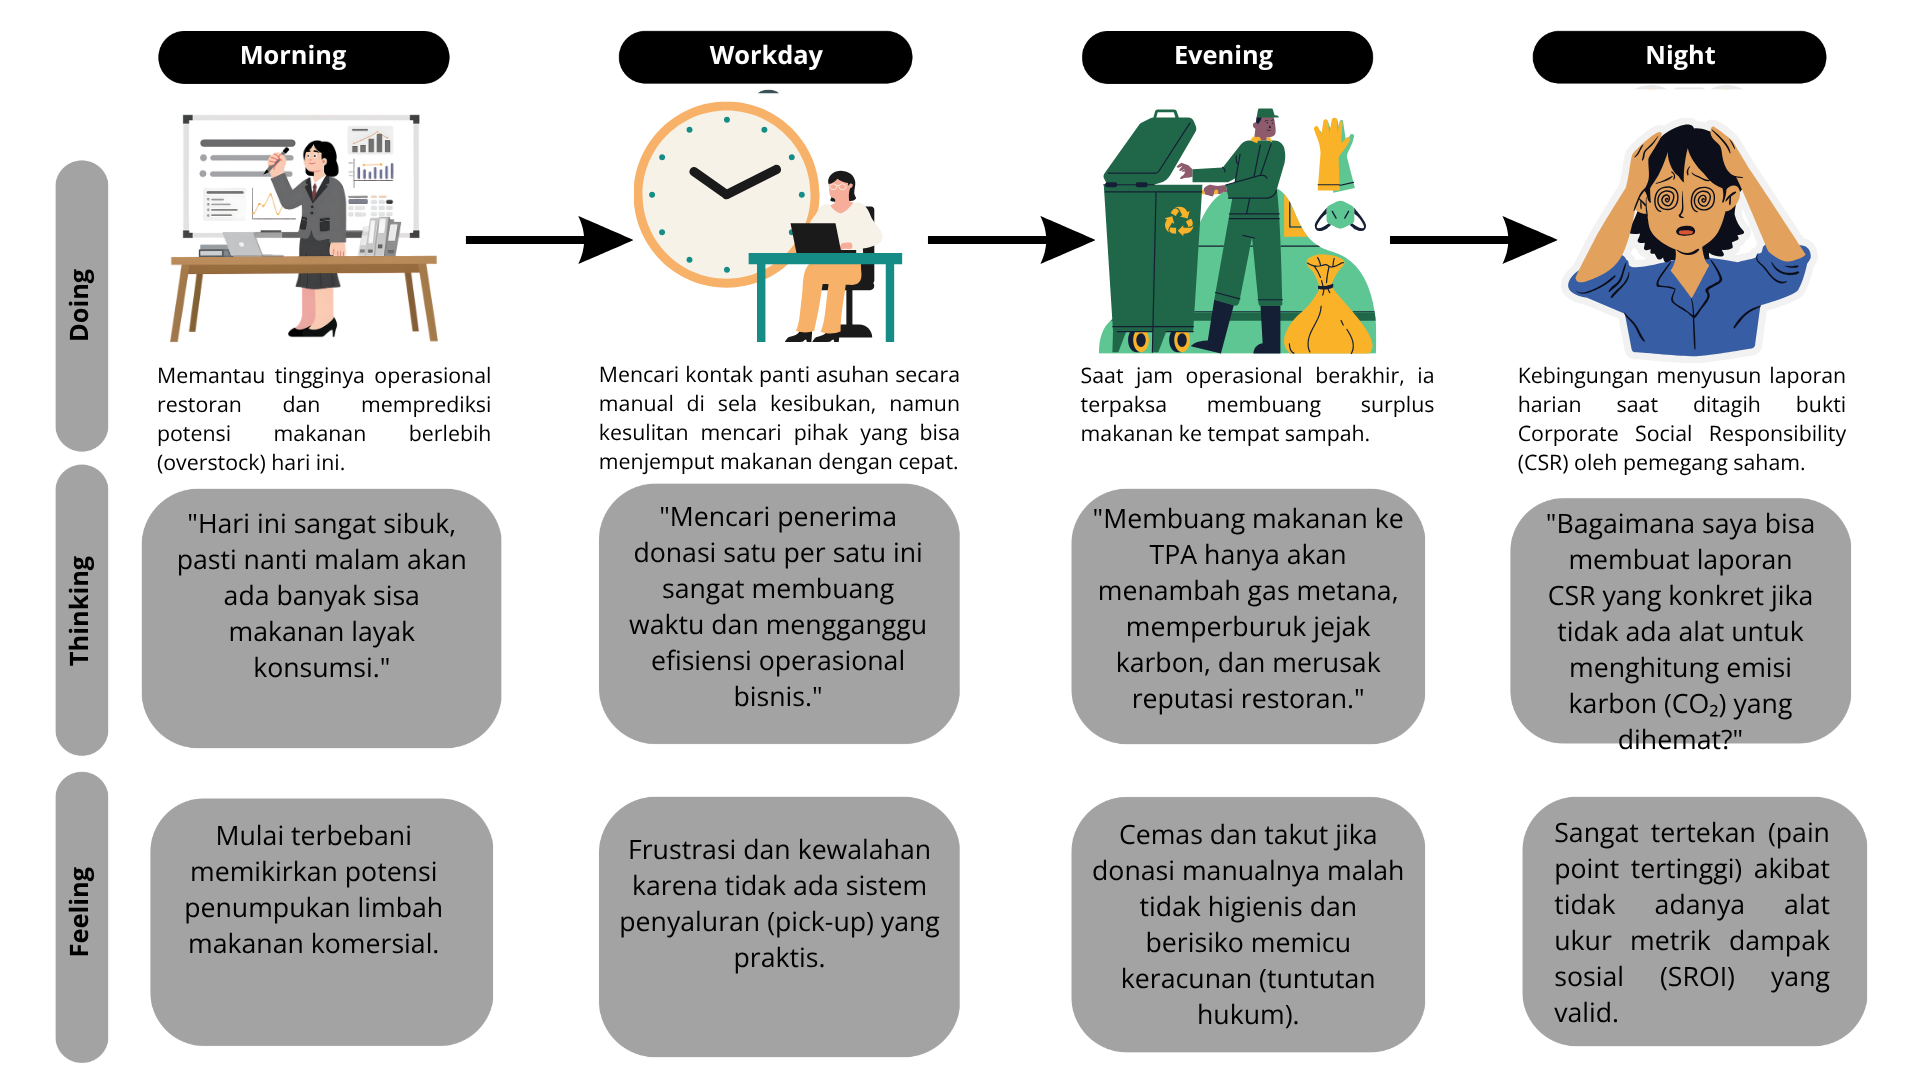
\includegraphics[width=0.99\textwidth]{image/bab2/segmentasi/CustomerJourneyMap/Salinan dari Template Journey Map/CJM_DONATUR_KORPORAT.png}
    \caption{Customer Journey Map Donatur Korporat}
    \label{fig:customerJourneyMapDonaturKorporat}
\end{figure}

Penjelasan Fase Customer Journey Map (Hendra): \\
\textit{Fase perjalanan: Prediksi Operasional $\rightarrow$ Pencarian Penerima Manual $\rightarrow$ Pembuangan Surplus $\rightarrow$ Kebingungan Pelaporan}
\begin{description}
    \item[Prediksi Operasional (Pagi):] Hendra mengawali hari dengan memantau padatnya operasional restoran. Ia sudah bisa memprediksi dan mulai terbebani memikirkan potensi penumpukan limbah makanan komersial (\textit{overstock}) di hari itu. Peluang Solusi (FAR): Login peran khusus korporat (RBAC) dengan dasbor prediksi volume surplus makanan untuk persiapan alokasi dini.
    \item[Pencarian Penerima Manual (Siang):] Di sela-sela kesibukan kerja, Hendra mencoba mencari kontak panti asuhan secara manual. Ia merasa frustrasi dan kewalahan karena sangat kesulitan menemukan pihak yang bisa menjemput makanan dengan cepat tanpa mengganggu efisiensi operasional bisnis. Peluang Solusi (FAR): Sistem otomatis (\textit{Missions Board}) yang menghubungkan tugas penjemputan logistik langsung ke Relawan Kurir.
    \item[Pembuangan Surplus (Sore):] Saat jam operasional berakhir, Hendra dilanda cemas dan takut mendonasikan makanannya secara manual. Tanpa standar higienitas, ia takut donasinya malah berisiko memicu keracunan dan tuntutan hukum. Akibatnya, ia terpaksa membuang surplus makanan tersebut ke TPA. Peluang Solusi (FAR): Fitur Wajib Pindai (\textit{Mandatory Scan}) QR Code dan validasi "Polisi Pangan" sebagai bukti serah terima yang aman secara hukum.
    \item[Kebingungan Pelaporan (Malam):] Hendra merasa sangat tertekan (\textit{Pain Point Tertinggi}) saat ditagih bukti pelaporan CSR oleh para pemegang saham. Ia kebingungan menyusun laporan harian yang konkret karena tidak adanya alat ukur untuk menghitung emisi karbon yang dihemat. Peluang Solusi (FAR): Dasbor SROI Korporat yang menyajikan angka penurunan emisi secara otomatis, terintegrasi dengan AI \textit{CSR Copywriter} untuk membuat laporan harian.
\end{description}

% \clearpage

\begin{figure}[H]
    \centering
    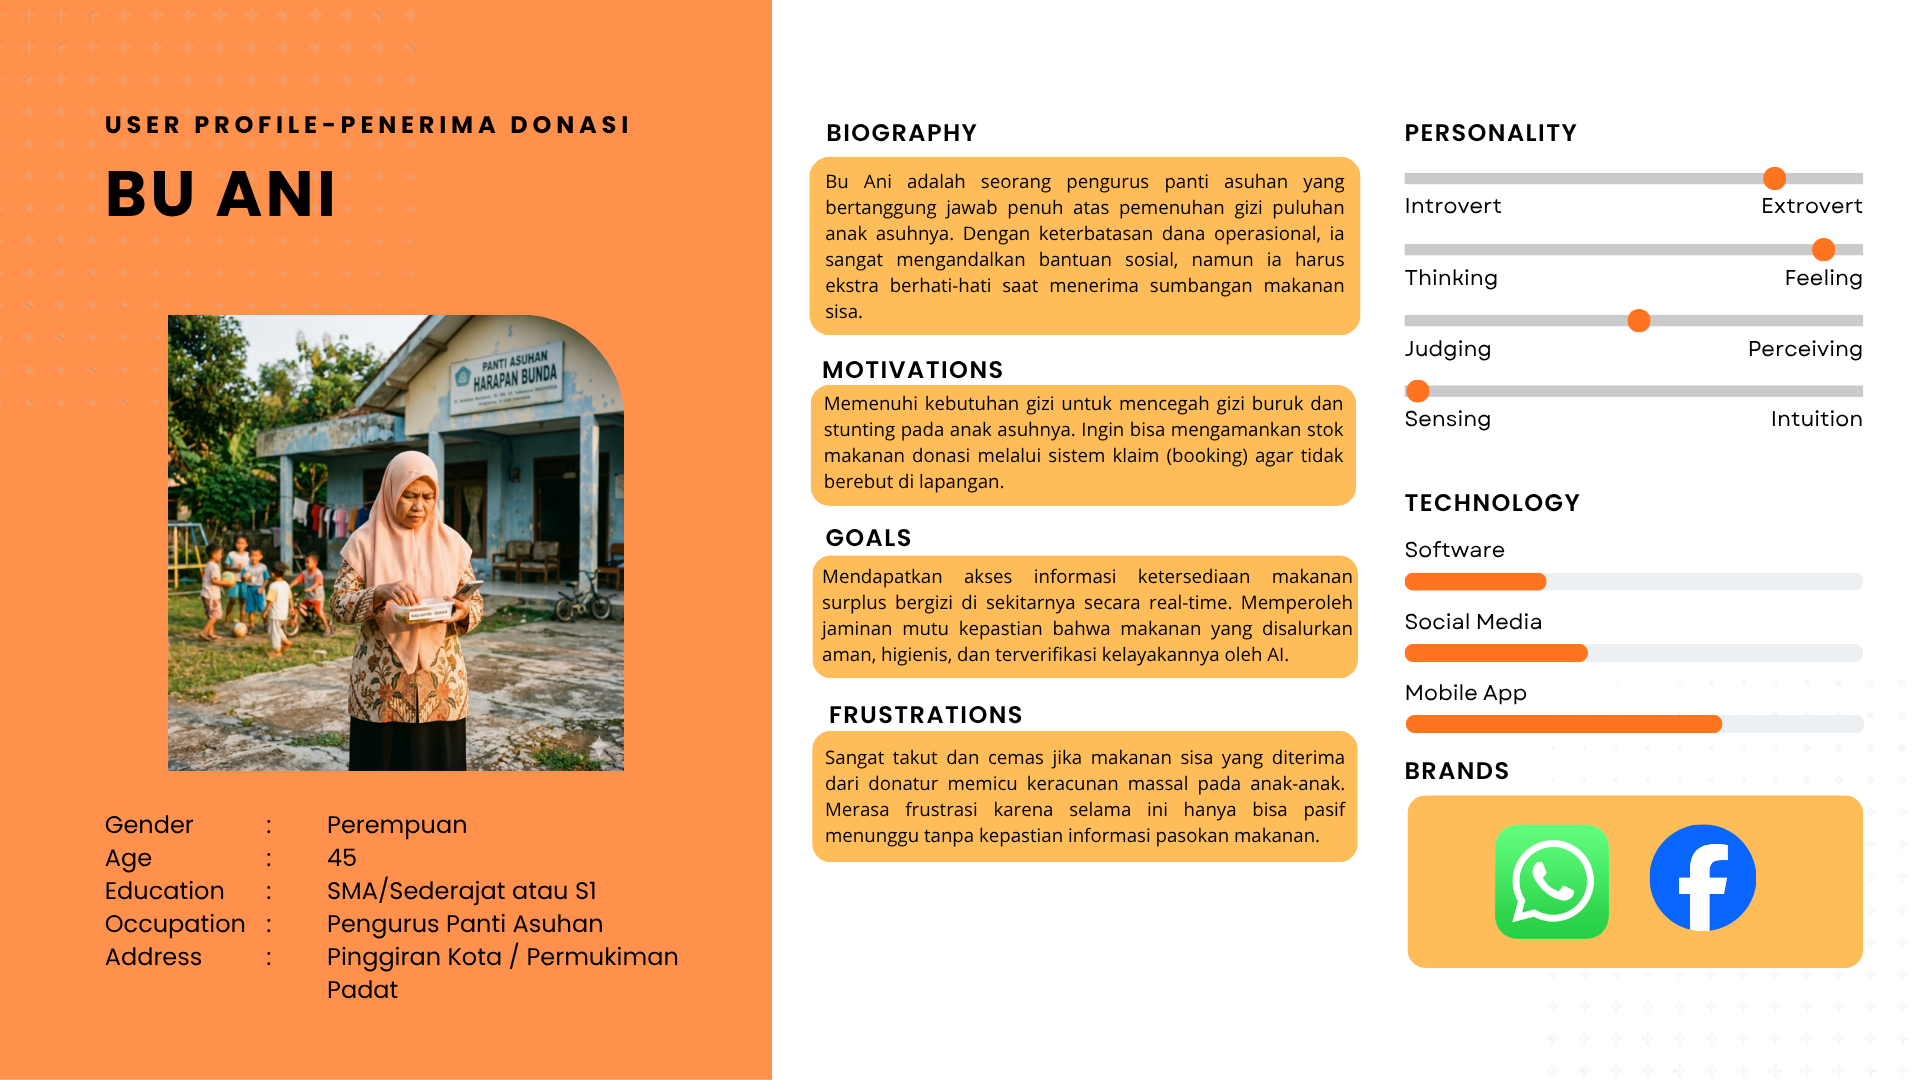
\includegraphics[width=1\textwidth]{image/bab2/segmentasi/UserPersona/Salinan dari baso arif/UP_PENERIMA DONASI.png}
    \caption{User Persona Penerima}
    \label{fig:userPersonaPenerima}
\end{figure}

Penjelasan Profil (Bu Ani):
Bu Ani (45 tahun) merupakan seorang pengurus panti asuhan di pinggiran kota/pemukiman padat. Ia memikul tanggung jawab penuh atas pemenuhan gizi puluhan anak asuhnya di tengah keterbatasan dana operasional.
\begin{itemize}
    \item Motivasi: Memenuhi kebutuhan gizi anak asuh demi mencegah kondisi gizi buruk dan \textit{stunting}. Ingin bisa mengamankan stok makanan donasi melalui sistem klaim (\textit{booking}) agar tidak perlu berebut di lapangan.
    \item Tujuan: Mendapatkan akses informasi terkait ketersediaan makanan surplus bergizi di sekitarnya secara \textit{real-time}, dengan jaminan mutu kepastian bahwa makanan tersebut aman, higienis, dan terverifikasi oleh AI.
    \item Frustrasi: Memiliki ketakutan mendalam jika makanan sisa yang diterima justru memicu keracunan massal pada anak-anak. Merasa frustrasi karena selama ini hanya bisa pasif menunggu bantuan tanpa kepastian pasokan.
    \item Preferensi: Aplikasi media sosial konvensional seperti WhatsApp dan Facebook.
\end{itemize}

\begin{figure}[H]
    \centering
    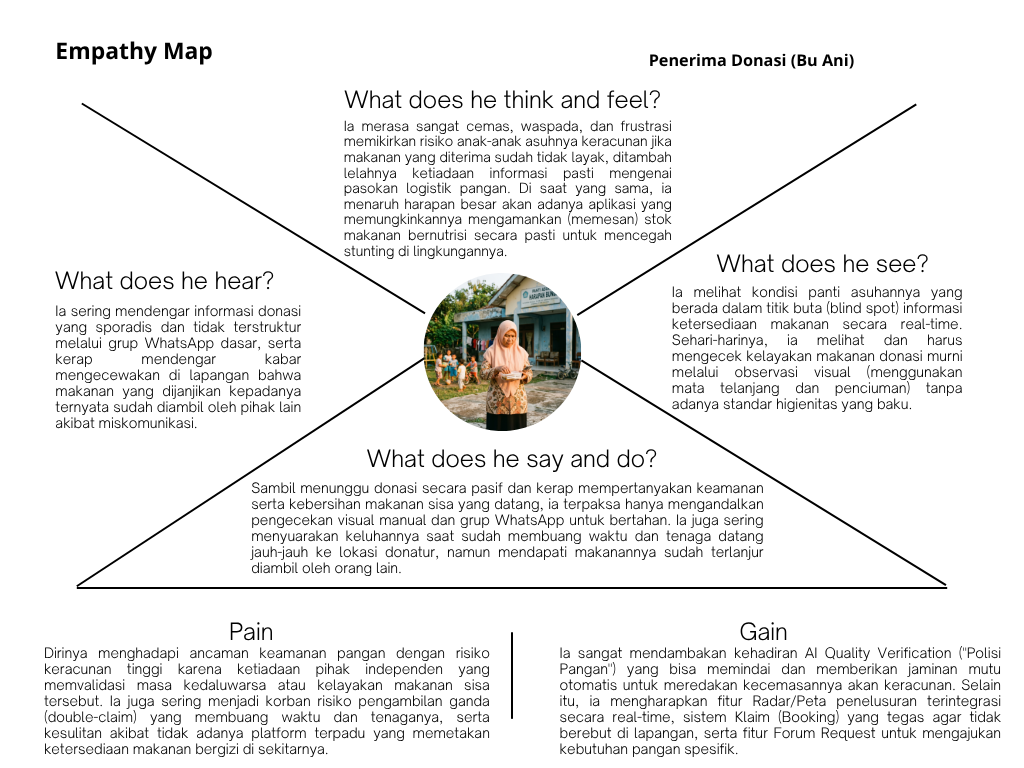
\includegraphics[width=1\textwidth]{image/bab2/segmentasi/EmpathyMap/Black and White Simple Empathy Map Brainstorm/EM_PENERIMA_DONASI.png}
    \caption{Empathy Map Penerima}
    \label{fig:empathyMapPenerima}
\end{figure}

Penjelasan Aspek Empathy Map (Bu Ani):
Bu Ani berada di pihak yang paling membutuhkan bantuan, namun juga pihak yang paling rentan terhadap risiko kesehatan dari makanan donasi.
\begin{itemize}
    \item THINKS \& FEELS: Merasa sangat cemas, waspada, dan didera frustrasi. Ia lelah dengan ketiadaan informasi pasti, ditambah memikirkan risiko anak asuhnya keracunan jika makanan yang diterima tidak layak. Ia menaruh harapan besar akan adanya aplikasi yang memungkinkannya mengamankan stok makanan bernutrisi secara pasti demi mencegah \textit{stunting}.
    \item HEARS: Kerap mendengar informasi donasi yang sporadis dan tidak terstruktur dari grup WhatsApp. Sayangnya, ia juga sering mendengar kabar mengecewakan di lapangan bahwa makanan yang dijanjikan sudah diambil oleh pihak lain akibat miskomunikasi.
    \item SEES: Menyadari kondisi panti asuhannya berada di titik buta (\textit{blind spot}) informasi ketersediaan makanan \textit{real-time}. Sehari-harinya, ia juga melihat dan harus mengecek kelayakan makanan murni melalui observasi visual manual (mata telanjang dan penciuman) tanpa standar higienitas baku.
    \item SAYS \& DOES: Sambil menunggu donasi secara pasif, ia hanya bisa mengandalkan pengecekan manual untuk bertahan. Ia kerap menyuarakan keluhan dan kekecewaannya saat sudah membuang tenaga dan waktu berjalan jauh, namun mendapati makanannya telah diambil orang lain.
    \item PAINS: Dirinya menghadapi ancaman keamanan pangan dengan risiko keracunan tinggi akibat ketiadaan alat validasi independen untuk makanan sisa. Ia sering menjadi korban perebutan/pengambilan ganda (\textit{double-claim}) yang membuang waktunya, serta kesulitan karena tidak ada platform peta terpadu ketersediaan makanan di sekitarnya.
    \item GAINS: Sangat mendambakan AI \textit{Quality Verification} ("Polisi Pangan") untuk menjamin mutu dan meredakan kecemasan akan keracunan. Ia juga mengharapkan fitur Peta Penelusuran \textit{real-time}, sistem Klaim (\textit{Booking}) agar tidak berebut di lapangan, serta Forum Request untuk mengajukan kebutuhan spesifik panti.
\end{itemize}

\begin{figure}[H]
    \centering
    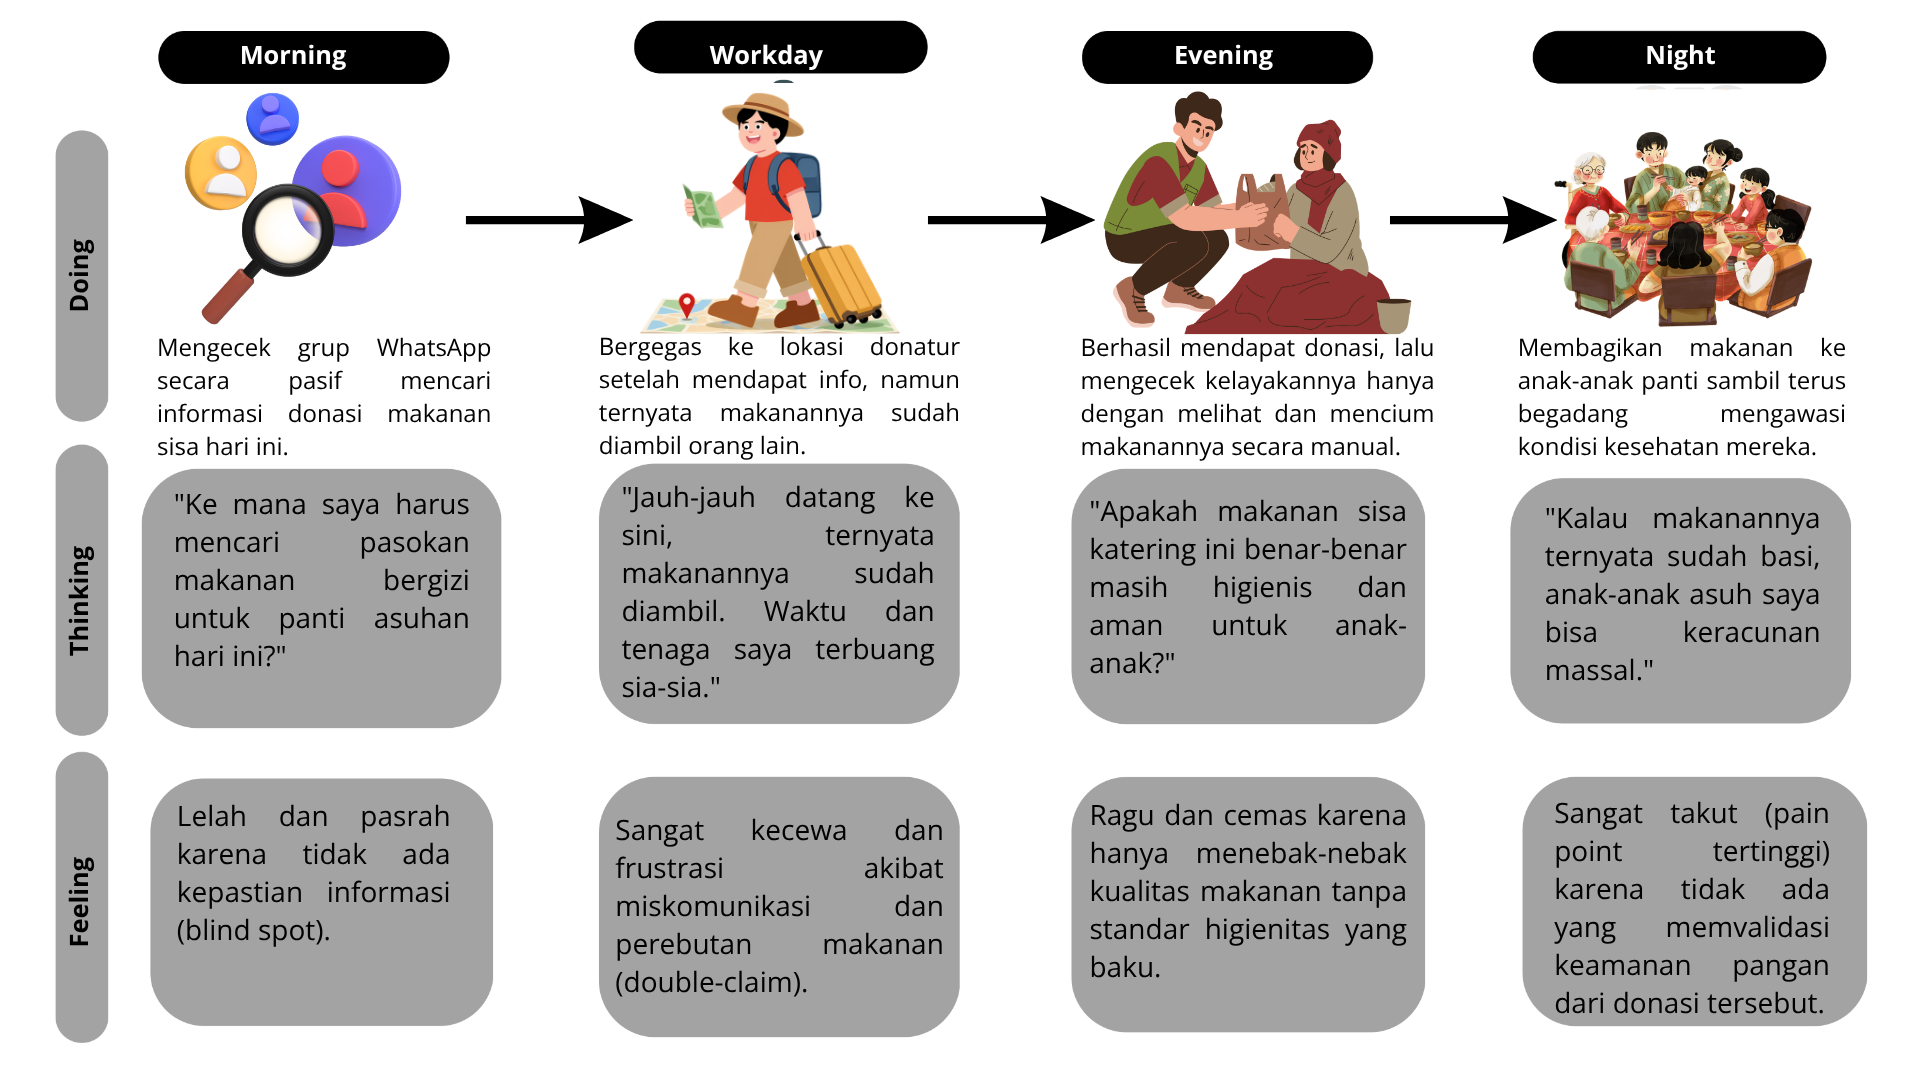
\includegraphics[width=0.99\textwidth]{image/bab2/segmentasi/CustomerJourneyMap/Salinan dari Template Journey Map/CJM_PENERIMA.png}
    \caption{Customer Journey Map Penerima}
    \label{fig:customerJourneyMapPenerima}
\end{figure}

Penjelasan Fase Customer Journey Map (Bu Ani): \\
\textit{Fase perjalanan: Pencarian Pasif $\rightarrow$ Pengejaran Donasi $\rightarrow$ Serah Terima Manual $\rightarrow$ Kekhawatiran Kesehatan}
\begin{description}
    \item[Pencarian Pasif (Pagi):] Bu Ani mengecek grup WhatsApp secara pasif untuk mencari informasi donasi makanan bergizi hari itu. Ia merasa lelah dan pasrah (\textit{Pain Points}) karena ketiadaan kepastian informasi (berada di \textit{blind spot}). Peluang Solusi (FAR): Fitur Peta Radar Penelusuran \textit{real-time} yang menampilkan ketersediaan donasi terdekat.
    \item[Pengejaran Donasi (Siang):] Bu Ani bergegas ke lokasi setelah mendapatkan info. Namun, ia sangat kecewa dan frustrasi (\textit{Pain Points}) karena makanannya ternyata sudah diambil orang lain akibat miskomunikasi dan perebutan makanan (\textit{double-claim}). Peluang Solusi (FAR): Fitur Sistem Klaim (\textit{Booking}) yang tegas sehingga makanan yang dipesan sudah "terkunci" untuknya.
    \item[Serah Terima Manual (Sore):] Ia akhirnya berhasil mendapat donasi. Namun, ia ragu dan cemas (\textit{Pain Points}) karena hanya bisa menebak-nebak kualitas makanan dengan melihat dan menciumnya tanpa adanya standar higienitas baku. Peluang Solusi (FAR): Proses verifikasi awal dari sisi donatur menggunakan AI \textit{Quality Verification}.
    \item[Kekhawatiran Kesehatan (Malam):] Bu Ani membagikan makanan ke anak-anak sambil begadang mengawasi kondisi mereka. Ia sangat takut (\textit{Pain Point Tertinggi}) bahwa kelalaiannya akan memicu keracunan massal karena tidak ada jaminan keamanan pangan. Peluang Solusi (FAR): Validasi "Polisi Pangan" yang memberi ketenangan batin (\textit{peace of mind}) secara mutlak.
\end{description}

% \clearpage

\begin{figure}[H]
    \centering
    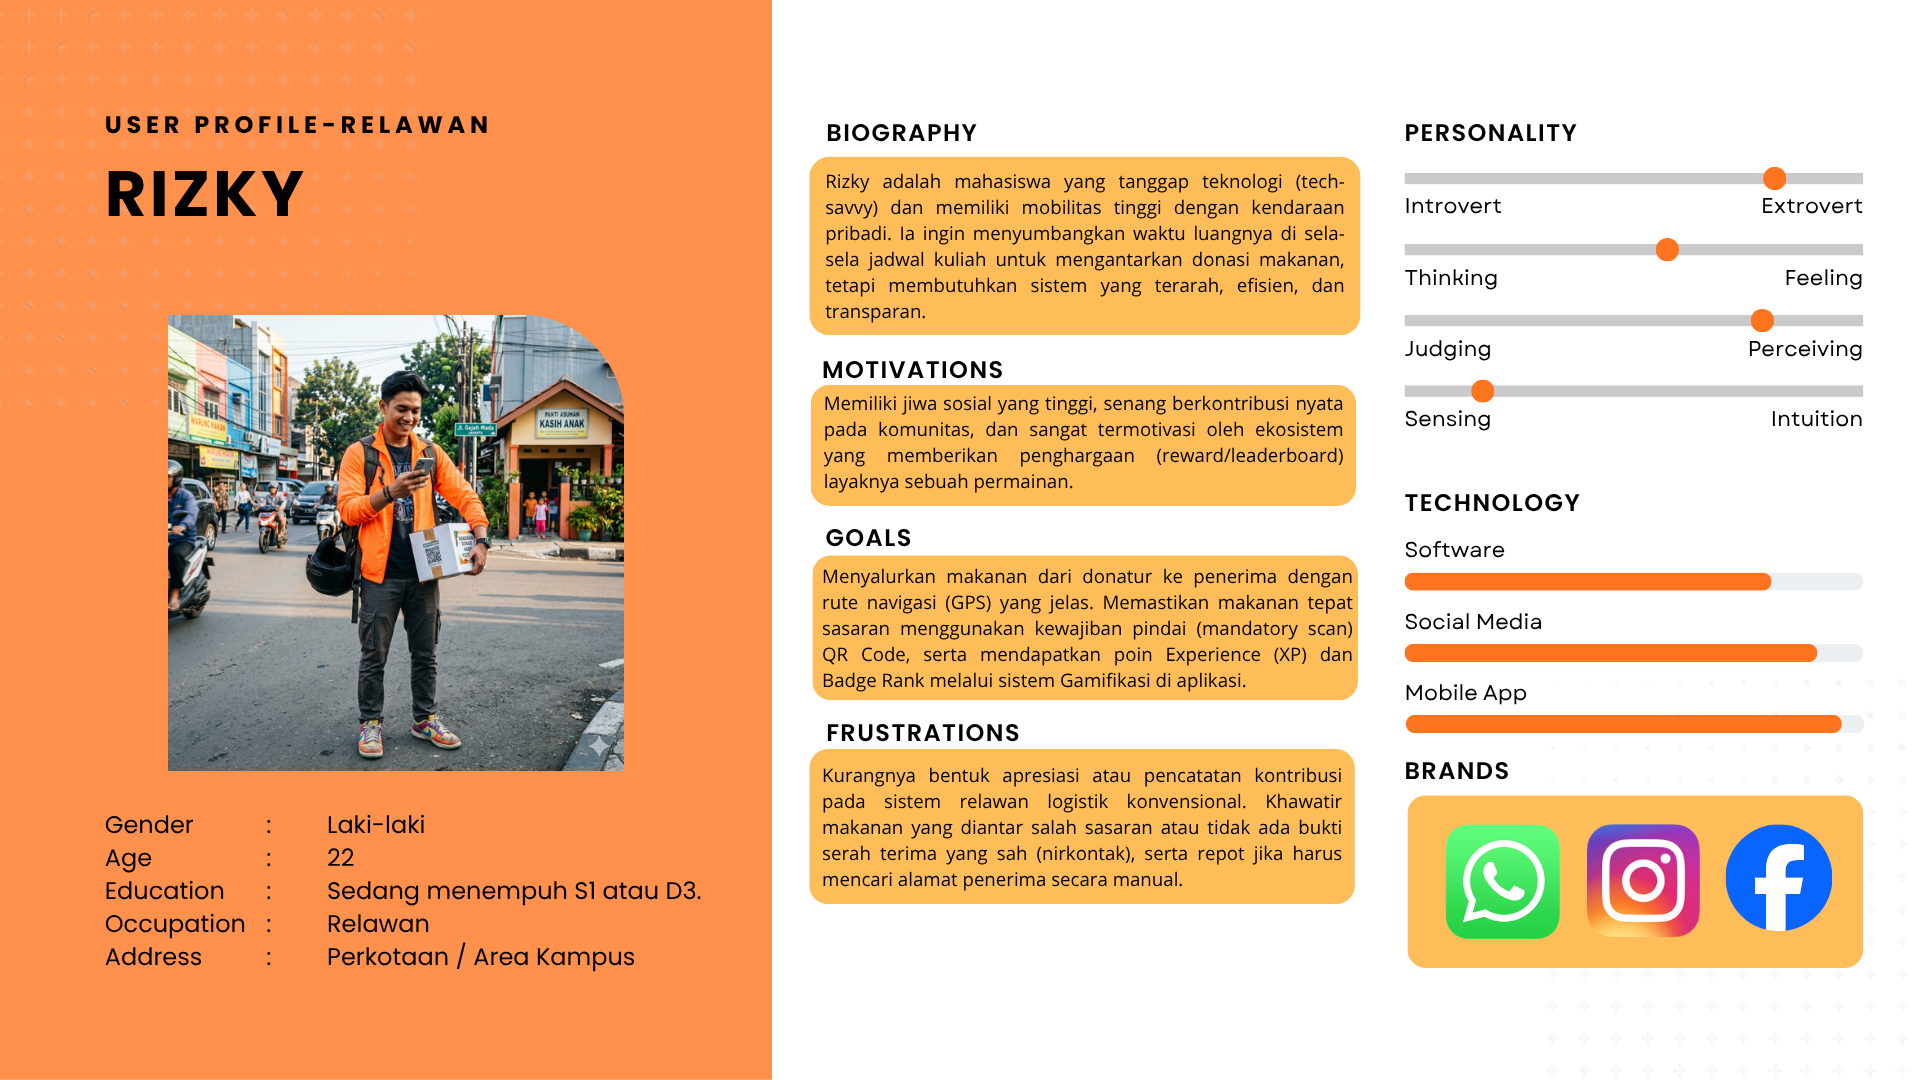
\includegraphics[width=1\textwidth]{image/bab2/segmentasi/UserPersona/Salinan dari baso arif/UP_RELAWAN.png}
    \caption{User Persona Relawan}
    \label{fig:userPersonaRelawan}
\end{figure}

Penjelasan Profil (Rizky):
Rizky (22 tahun) adalah seorang mahasiswa (\textit{tech-savvy}) dengan tingkat mobilitas tinggi menggunakan kendaraan pribadinya. Di sela-sela kepadatan jadwal kuliahnya, ia ingin menyumbangkan waktu luangnya untuk menjadi kurir logistik donasi makanan.
\begin{itemize}
    \item Motivasi: Memiliki jiwa sosial yang tinggi, senang berkontribusi nyata pada komunitas, dan sangat termotivasi oleh ekosistem yang memberikan penghargaan (\textit{reward/leaderboard}) layaknya sebuah permainan.
    \item Tujuan: Menyalurkan makanan dari donatur ke penerima menggunakan rute navigasi (GPS) yang jelas. Ia juga ingin memastikan makanan tepat sasaran menggunakan kewajiban pindai (\textit{mandatory scan}) QR Code, serta mendapatkan poin \textit{Experience} (XP) dan \textit{Badge Rank} melalui sistem gamifikasi.
    \item Frustrasi: Kurangnya bentuk apresiasi atau pencatatan kontribusi pada sistem relawan konvensional. Ia juga repot jika harus mencari alamat secara manual dan selalu khawatir makanan yang diantar salah sasaran tanpa adanya bukti serah terima yang sah.
    \item Preferensi: Aplikasi \textit{mobile}, perangkat lunak navigasi, media sosial, dan gamifikasi.
\end{itemize}

\begin{figure}[H]
    \centering
    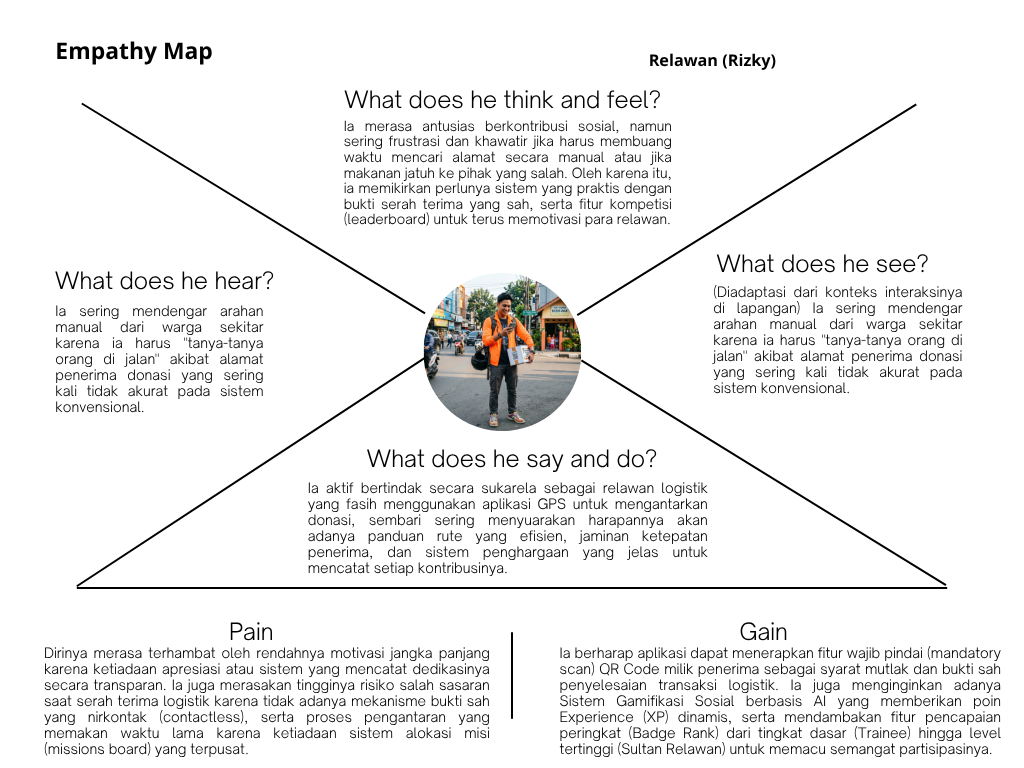
\includegraphics[width=1\textwidth]{image/bab2/segmentasi/EmpathyMap/Black and White Simple Empathy Map Brainstorm/EM_RELAWAN.png}
    \caption{Empathy Map Relawan}
    \label{fig:empathyMapRelawan}
\end{figure}

Penjelasan Aspek Empathy Map (Rizky):
Rizky merepresentasikan relawan muda yang bersemangat, namun kerap terhambat oleh inefisiensi sistem manual di lapangan.
\begin{itemize}
    \item THINKS \& FEELS: Merasa sangat antusias untuk berkontribusi sosial, namun sering dirundung frustrasi dan khawatir jika harus membuang waktu mencari alamat secara manual atau jika makanannya jatuh ke pihak yang salah. Ia memikirkan perlunya sistem praktis dengan bukti serah terima sah serta fitur kompetisi (\textit{leaderboard}) untuk memotivasinya.
    \item HEARS: Sering mendengar arahan manual dari warga sekitar karena ia harus "tanya-tanya orang di jalan" akibat titik alamat penerima donasi yang sering kali tidak akurat pada sistem konvensional.
    \item SEES: Dalam interaksinya di lapangan, ia melihat secara langsung betapa tidak akuratnya sistem alamat konvensional, sehingga ia berulang kali dihadapkan pada situasi harus mengandalkan arahan manual warga sekitar.
    \item SAYS \& DOES: Bertindak aktif secara sukarela sebagai relawan logistik yang fasih menggunakan aplikasi GPS. Sembari bekerja, ia sering menyuarakan harapannya akan adanya panduan rute efisien, jaminan ketepatan penerima, dan sistem penghargaan yang mencatat setiap kontribusinya.
    \item PAINS: Merasa terhambat oleh rendahnya motivasi jangka panjang akibat ketiadaan apresiasi dan pencatatan dedikasi transparan. Ia mengalami proses pengantaran yang memakan waktu lama karena ketiadaan sistem alokasi misi (\textit{missions board}) terpusat, serta tingginya risiko salah sasaran tanpa mekanisme bukti sah serah terima.
    \item GAINS: Berharap ada fitur Wajib Pindai (\textit{mandatory scan}) QR Code milik penerima sebagai syarat mutlak penyelesaian transaksi logistik. Ia juga sangat menginginkan Sistem Gamifikasi Sosial berbasis AI yang memberikan XP dinamis dan \textit{Badge Rank} (dari tingkat dasar/Trainee hingga Sultan Relawan).
\end{itemize}

\begin{figure}[H]
    \centering
    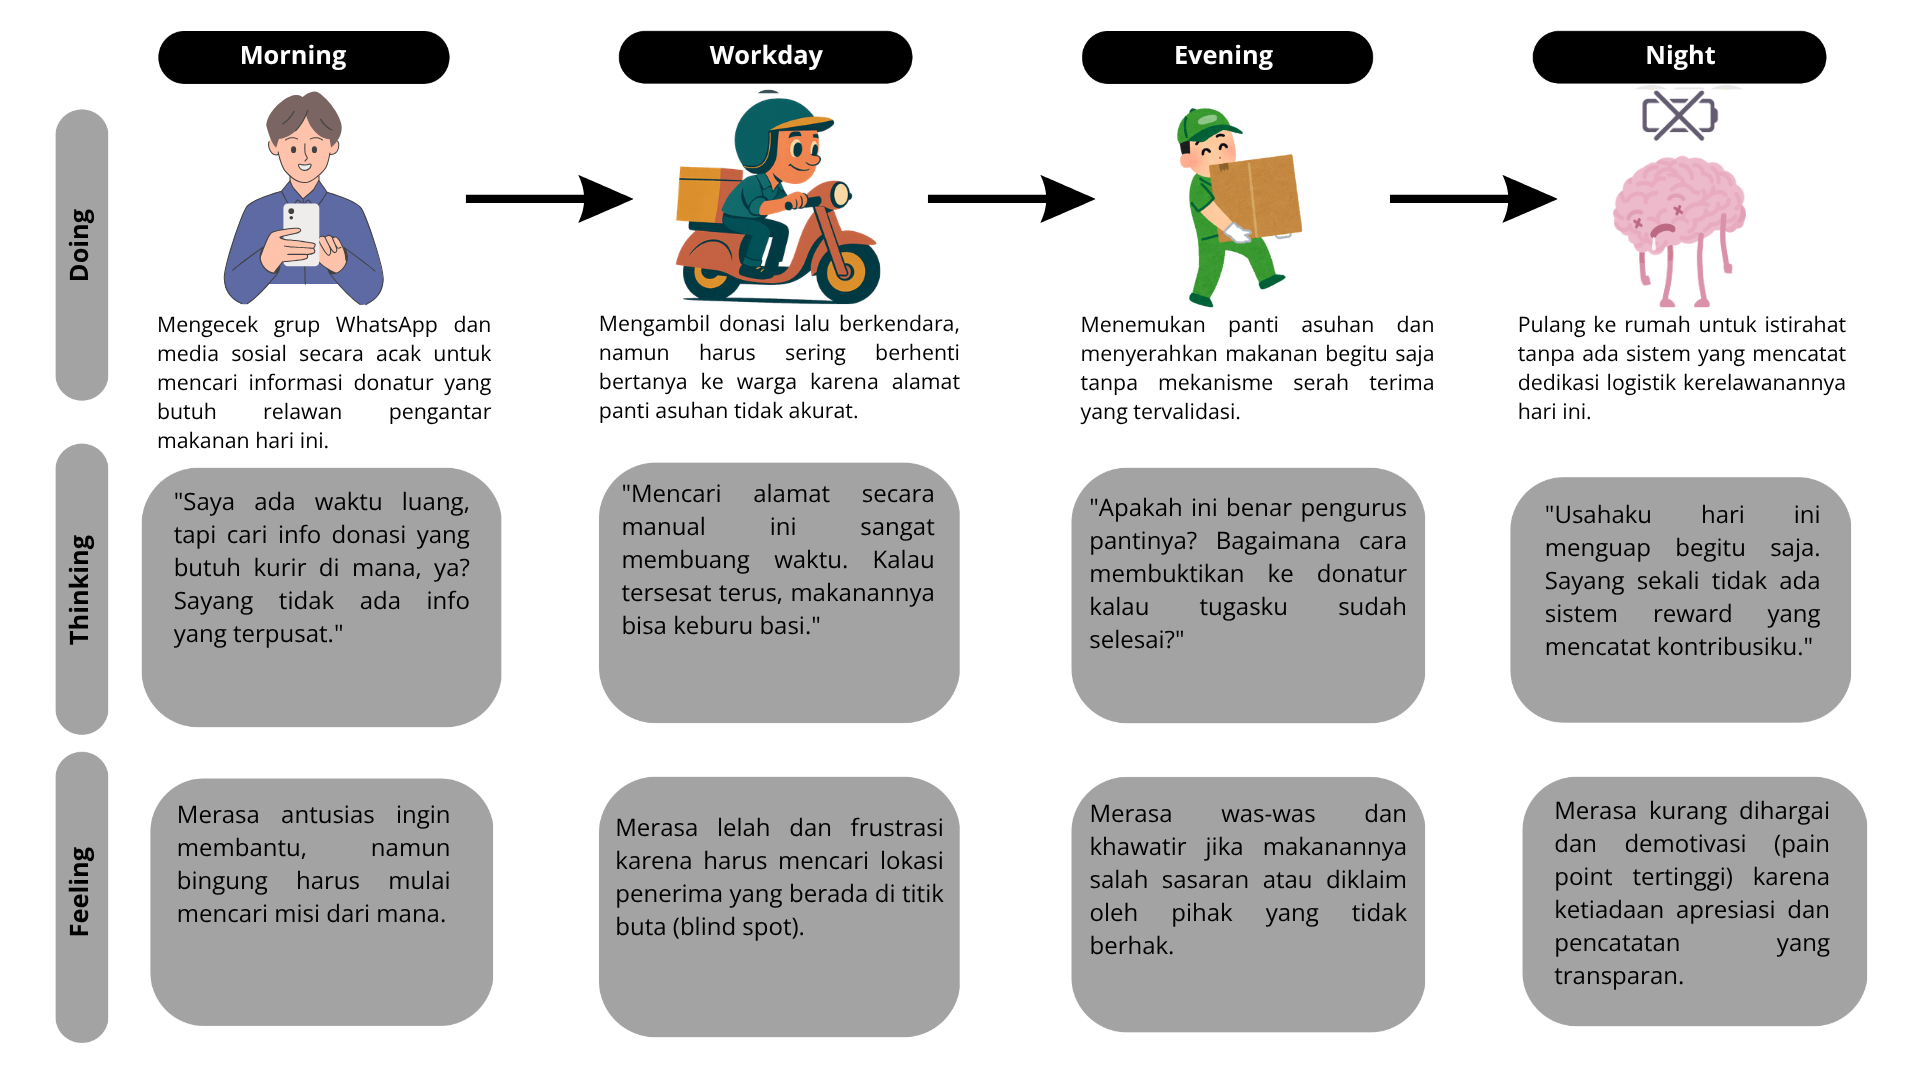
\includegraphics[width=0.85\textwidth]{image/bab2/segmentasi/CustomerJourneyMap/Salinan dari Template Journey Map/CJM_RELAWAN.png}
    \caption{Customer Journey Map Relawan}
    \label{fig:customerJourneyMapRelawan}
\end{figure}

Penjelasan Fase Customer Journey Map (Rizky): \\
\textit{Fase perjalanan: Pengecekan Misi $\rightarrow$ Penjemputan \& Pengantaran $\rightarrow$ Serah Terima Makanan $\rightarrow$ Pasca-Kerelawanan}
\begin{description}
    \item[Pengecekan Misi (Pagi):] Rizky memiliki waktu luang dan mengecek grup WhatsApp serta media sosial secara pasif untuk mencari donatur yang butuh kurir. Ia merasa antusias namun kebingungan (\textit{Pain Points}) karena informasi tidak terpusat. Peluang Solusi (FAR): Fitur \textit{Missions Board} terpusat yang menampilkan daftar penugasan logistik harian.
    \item[Penjemputan \& Pengantaran (Siang):] Rizky berkendara mengambil donasi, namun sering tersesat. Ia merasa lelah dan frustrasi (\textit{Pain Points}) karena mencari alamat manual di titik buta sangat membuang waktu dan berisiko membuat makanan keburu basi. Peluang Solusi (FAR): Navigasi GPS terintegrasi yang akurat menuju titik donatur dan penerima.
    \item[Serah Terima Makanan (Sore):] Rizky berhasil menemukan panti asuhan, namun merasa was-was dan khawatir (\textit{Pain Points}) menyerahkan makanan begitu saja karena tidak ada mekanisme validasi bahwa orang tersebut berhak menerimanya. Peluang Solusi (FAR): \textit{Mandatory Scan} QR Code nirkontak sebagai validasi serah terima yang mutlak.
    \item[Pasca-Kerelawanan (Malam):] Rizky pulang untuk istirahat. Ia merasa kurang dihargai dan sangat demotivasi (\textit{Pain Point Tertinggi}) karena dedikasi logistiknya menguap begitu saja tanpa ada sistem \textit{reward} atau pencatatan transparan. Peluang Solusi (FAR): Sistem Gamifikasi yang memberikan XP dan \textit{Badge Rank} seketika setelah misi selesai.
\end{description}
% \clearpage

\section{Identifikasi Aplikasi Sejenis}
\par Tahapan identifikasi aplikasi sejenis merupakan langkah analitis yang dilakukan untuk memetakan produk atau platform digital pendahulu (\textit{existing solutions}) yang memiliki kesamaan fungsional dengan sistem yang diusulkan. Tujuan utama dari observasi ini adalah untuk menemukan celah kelemahan (\textit{gap}) serta batasan operasional pada aplikasi yang telah beredar di masyarakat. Melalui analisis komparatif ini, pengembangan platform Food AI Rescue dapat difokuskan untuk merancang nilai tambah (\textit{value proposition}) yang lebih inovatif, tepat sasaran, dan relevan dalam menjembatani kebutuhan para pemangku kepentingan di ekosistem donasi pangan.

\par Dalam observasi ini, perbandingan difokuskan pada empat platform pengelola sisa makanan yang menjadi tolok ukur dalam inisiatif food rescue, yaitu:
\begin{enumerate}
    \item Surplus Indonesia: Aplikasi \textit{food rescue} komersial yang berfokus menyelamatkan makanan berlebih dari pelaku usaha (restoran, hotel, katering) dengan memfasilitasi pelanggan untuk membeli makanan yang belum habis terjual tersebut di akhir jam operasional dengan potongan harga hingga setengahnya.
    \item Garda Pangan: Organisasi \textit{food bank} di Indonesia yang berfokus pada penyelamatan surplus makanan dari industri \textit{hospitality} dan mendistribusikannya secara gratis kepada masyarakat pra-sejahtera melalui operasional jaringan relawan secara konvensional.
    \item Foodbank of Indonesia (FOI): Jaringan nirlaba nasional yang mengelola distribusi donasi dan makanan berlebih dari berbagai pihak untuk mencegah kelaparan, dengan fokus kampanye pada perbaikan gizi anak-anak balita dan kelompok rentan di berbagai wilayah.
    \item Too Good To Go: Aplikasi global pionir \textit{food rescue} (populer di Eropa dan Amerika) yang menghubungkan pelanggan dengan restoran atau toko kelontong untuk membeli ``paket kejutan'' (\textit{magic bags}) berisi makanan sisa layak konsumsi dengan harga yang sangat murah.
\end{enumerate}

\par Rincian perbandingan fitur dan kapabilitas layanan antara platform kompetitor dengan sistem Food AI Rescue yang diusulkan dapat diringkas pada tabel berikut:

\begin{table}[htbp]
    \centering
    \renewcommand{\arraystretch}{1.5}
    \caption{Perbandingan Fitur dan Kapabilitas Layanan Platform Food Rescue}
    \label{tab:perbandingan_fitur}
    \begin{tabularx}{\textwidth}{|L|C|C|C|C|C|}
        \hline
        \rowcolor{gray!10} Fitur / Layanan Utama & Surplus Indonesia & Garda Pangan & Foodbank of Indonesia & Too Good To Go & Food AI Rescue (Usulan) \\ \hline
        Penyaluran Donasi Makanan Secara Gratis & \xmark & \cmark & \cmark & \xmark & \cmark \\ \hline
        Verifikasi Kelayakan Makanan Otomatis (AI) & \xmark & \xmark & \xmark & \xmark & \cmark \\ \hline
        Sistem Penjemputan oleh Relawan Tergamifikasi & \xmark & \xmark & \xmark & \xmark & \cmark \\ \hline
        Validasi Serah Terima Nirkontak (QR Code) & \xmark & \xmark & \xmark & \xmark & \cmark \\ \hline
        Dasbor Kalkulasi Dampak Sosial (SROI) \textit{Real-Time} & \xmark & \xmark & \xmark & \xmark & \cmark \\ \hline
        Fitur AI Generatif untuk Kampanye CSR Korporat & \xmark & \xmark & \xmark & \xmark & \cmark \\ \hline
    \end{tabularx}
\end{table}

\newpage

\par Berdasarkan Tabel \ref{tab:perbandingan_fitur} di atas, dapat diidentifikasi beberapa celah (\textit{gap}) fungsionalitas yang menjadi landasan utama pengembangan Food AI Rescue. Platform komersial seperti Surplus Indonesia dan Too Good To Go sangat unggul dalam menyelamatkan sisa makanan dengan cepat, namun berfokus pada model transaksi jual-beli diskon, sehingga belum sepenuhnya menyasar masyarakat prasejahtera yang membutuhkan donasi secara cuma-cuma. Sementara itu, inisiatif sosial seperti Garda Pangan dan Foodbank of Indonesia memiliki rekam jejak penyaluran donasi gratis yang sangat baik, namun operasional logistiknya masih bersifat konvensional dan sangat bergantung pada verifikasi kelayakan makanan secara manual oleh manusia.

\par Lebih jauh lagi, keempat platform pembanding tersebut umumnya belum mengadopsi teknologi mutakhir seperti Kecerdasan Buatan (AI). Belum tersedia fitur otomatisasi yang mampu memverifikasi standar keamanan dan higienitas makanan secara visual (\textit{Computer Vision}), serta belum ada pelacakan metrik dampak lingkungan yang komprehensif. Platform pendahulu juga belum menyediakan dukungan fitur khusus yang memfasilitasi kebutuhan pelaporan donatur korporat dalam satu pusat kendali (\textit{dashboard}).

\par Oleh karena itu, usulan pengembangan Food AI Rescue hadir dengan posisi tawar (\textit{value proposition}) yang unik. Food AI Rescue menggabungkan penyaluran donasi pangan gratis, validasi keamanan berbasis AI (``Polisi Pangan''), dan operasional penjemputan logistik berbasis gamifikasi relawan ke dalam satu aplikasi yang ramah pengguna. Keberadaan Dasbor Dampak Sosial (SROI) \textit{real-time} serta pemisahan hak akses berbasis peran (\textit{Role-Based Access Control}) antara donatur, penerima, relawan, dan admin menjadikan platform ini tidak hanya sebagai alat penyalur bantuan teknis, tetapi juga sebagai ekosistem manajemen komunitas ketahanan pangan cerdas yang aman, transparan, dan terpadu.

\section{Analisis Kebutuhan Sistem}
Analisis persyaratan sistem merupakan langkah esensial dalam mentransformasikan kendala operasional pada sistem manual (As-Is) serta titik keluhan (pain points) para aktor lapangan ke dalam spesifikasi teknis yang komprehensif bagi platform Food AI Rescue. Tahapan analisis ini diklasifikasikan ke dalam tiga segmen utama, yakni pendefinisian tingkat hak akses pengguna (meliputi Donatur, Penerima, Relawan, Admin, dan SuperAdmin), pemetaan kebutuhan fungsional cerdas aplikasi, serta spesifikasi infrastruktur teknologi pendukung di sisi backend.

\subsection{Analisis Grup Akses}
\par Berdasarkan deskripsi pengguna dan pemetaan empati dari hasil rancangan \textit{User Persona}, terlihat jelas bahwa pengguna pada ekosistem aplikasi ini memiliki latar belakang literasi teknologi serta tanggung jawab operasional yang sangat bervariasi. Untuk mencegah pengguna awam kebingungan saat menavigasi fitur aplikasi, serta guna melindungi stabilitas infrastruktur sistem, seperti basis data dan konfigurasi Kecerdasan Buatan (AI), dari risiko penyalahgunaan atau kesalahan pengaturan (\textit{human error}), maka platform Food AI Rescue dirancang menggunakan arsitektur keamanan \textit{Role-Based Access Control} (RBAC).

\par Sistem ini membagi pengguna ke dalam 6 (enam) grup akses (\textit{role}) utama dengan pembatasan wewenang, fungsionalitas, dan pemanfaatan Kecerdasan Buatan (AI) yang sangat spesifik, yaitu:

\begin{enumerate}
    \item Donatur Individu
    \begin{itemize}
        \item Peranan: Pengguna dari kalangan masyarakat perorangan atau pelaku usaha skala mikro yang memiliki kelebihan produksi makanan layak konsumsi dalam jumlah kecil (skala rumah tangga).
        \item Hak Akses: Memiliki wewenang operasional untuk mengunggah data makanan surplus, memperbarui status ketersediaan (\textit{inventory}), dan melakukan serah terima donasi dengan wajib memindai Kode QR milik penerima sebagai bukti sah. Donatur individu juga berhak memantau Dasbor Dampak Sosial (SROI) secara langsung, serta menggunakan hak akses AI \textit{Quality Verification} (Polisi Pangan) untuk memvalidasi kelayakan makanan dan mendapatkan rekomendasi resep masakan.
    \end{itemize}

    \item Donatur Kelompok/Korporat (Mitra Penyedia)
    \begin{itemize}
        \item Peranan: Pengguna dari entitas bisnis skala besar, khususnya di sektor HORECA (Hotel, Restoran, dan Kafe), atau usaha katering berskala komersial yang menyumbangkan surplus makanan secara masif.
        \item Hak Akses: Memiliki wewenang manajemen distribusi dan pemantauan SROI yang sama dengan Donatur Individu. Sebagai nilai tambah untuk kebutuhan \textit{Corporate Social Responsibility} (CSR), peran ini dibekali hak akses AI Generatif eksklusif yang meliputi fitur \textit{Eco Packaging Editor} untuk merancang desain kemasan ramah lingkungan, dan fitur \textit{CSR Copywriter} untuk otomatisasi pembuatan naskah kampanye sosial.
    \end{itemize}

    \item Penerima (Mitra Penerima)
    \begin{itemize}
        \item Peranan: Kelompok masyarakat di kawasan rentan pangan, fasilitas sosial (seperti panti asuhan), dewan kemakmuran masjid (DKM), atau warga prasejahtera yang bertindak sebagai sasaran distribusi donasi.
        \item Hak Akses: Memiliki wewenang untuk mengakses radar peta (\textit{Map Dashboard}), mencari menu makanan terdekat, melakukan klaim (\textit{booking}) guna mencegah pengambilan ganda (\textit{double-claim}), dan menyajikan Kode QR miliknya untuk dipindai saat makanan tiba. Grup ini juga diberi hak untuk memberikan ulasan (\textit{feedback}), mengajukan permintaan spesifik via \textit{Forum Request}, serta menggunakan AI \textit{Quality Verification} untuk mengecek makanan sebelum dikonsumsi.
    \end{itemize}

    \item Relawan (Kurir)
    \begin{itemize}
        \item Peranan: Pengguna dari kalangan pemuda lokal atau masyarakat umum yang berpartisipasi secara sukarela (\textit{crowdsourcing}) sebagai armada penggerak logistik sosial penjemputan makanan.
        \item Hak Akses: Berwenang untuk mengakses daftar papan misi pengantaran, melakukan penjemputan makanan dari lokasi donatur, dan mengantarkannya ke titik lokasi penerima. Relawan memegang otoritas validasi lapangan dengan hak akses wajib pindai (\textit{mandatory scan}) Kode QR nirkontak sebagai syarat mutlak penyelesaian transaksi, yang secara otomatis terintegrasi dengan sistem poin gamifikasi (\textit{Leaderboard Ranking}).
    \end{itemize}

    \item Admin Pengelola
    \begin{itemize}
        \item Peranan: Tim manajerial dan pengawas operasional harian yang bertugas mengelola platform secara administratif di tingkat komunitas.
        \item Hak Akses: Memiliki wewenang administratif untuk memverifikasi pendaftaran akun baru, memblokir akun yang melakukan penyalahgunaan, menangani keluhan pengguna (\textit{support request}), serta memantau Dasbor Statistik (SROI) dan peta panas (\textit{heatmap}) sebaran donasi. Dari sisi kecerdasan buatan, Admin dibekali hak modifikasi panel \textit{Prompt Engineering} untuk menyesuaikan parameter instruksi deteksi AI secara \textit{real-time} tanpa perlu mengubah kode sumber aplikasi.
    \end{itemize}

    \item Super Admin
    \begin{itemize}
        \item Peranan: Pengguna dengan tingkat literasi teknologi tertinggi yang bertindak sebagai pengembang sistem (Tim IT / \textit{Programmer}) dan pemegang kedaulatan mutlak platform eksekutif.
        \item Hak Akses: Memiliki wewenang manajerial penuh terhadap operasional sistem di sisi peladen (\textit{backend}). Akses difokuskan pada manajemen tingkat makro seperti pemeliharaan server (\textit{Maintenance Mode}), perbaikan \textit{bug}, menjaga stabilitas basis data, mengelola pendaftaran akun Admin biasa, serta mengawasi hak prerogatif akses komputasi AI dan memonitor jejak \textit{log} sistem secara keseluruhan.
    \end{itemize}
\end{enumerate}

\subsection{Analisis Kebutuhan Fungsional}
Analisis kebutuhan fungsional menguraikan spesifikasi kapabilitas yang wajib dimiliki oleh sistem guna menjawab permasalahan pengguna di lapangan. Merujuk pada hasil observasi alur distribusi manual (As-Is) serta ekstraksi titik keluhan (\textit{pain points}) dari \textit{Empathy Map} dan \textit{User Journey Map}, platform yang dirancang harus mampu menghadirkan solusi berupa otomatisasi verifikasi kelayakan pangan berbasis Kecerdasan Buatan (AI), pencocokan donasi secara \textit{real-time}, serta rekapitulasi pelaporan dampak lingkungan (SROI) secara digital. Oleh karena itu, fungsionalitas yang akan diimplementasikan pada ekosistem Food AI Rescue diklasifikasikan ke dalam tujuh modul utama berikut:

\begin{enumerate}
    \item Kebutuhan Modul Autentikasi dan Manajemen Akun
    \begin{itemize}
        \item Sistem harus mampu memfasilitasi proses pendaftaran (\textit{register}) dan masuk (\textit{login}) yang keamanannya terenkripsi menggunakan algoritma sandi berlapis \textit{bcrypt}.
        \item Sistem harus memiliki pendeteksi perutean berbasis peran (\textit{Role-Based Router}) untuk mengarahkan pengguna secara spesifik ke antarmuka 6 (enam) grup akses yang berbeda (Donatur Individu, Donatur Korporat, Penerima, Relawan, Admin, dan SuperAdmin).
        \item Sistem harus menyediakan fitur manajemen profil pengguna, yang mencakup utilitas pemotongan gambar (\textit{crop image}) saat pengguna mengunggah foto \textit{avatar}.
    \end{itemize}

    \item Kebutuhan Modul Manajemen Donasi dan Inventori (Gudang Pangan)
    \begin{itemize}
        \item Sistem harus memfasilitasi pihak Donatur untuk membuat daftar donasi makanan baru beserta detail parameter minimum dan maksimum porsi yang tersedia.
        \item Sistem harus dilengkapi dengan manajemen inventori otomatis yang mampu menyembunyikan status tayangan donasi dari publik apabila batas waktu konsumsi (kedaluwarsa) telah terlewati.
        \item Sistem harus memfasilitasi donatur untuk melakukan validasi serah terima melalui fitur pemindaian Kode QR penerima secara nirkontak saat proses penyerahan berlangsung.
    \end{itemize}

    \item Kebutuhan Modul Integrasi Kecerdasan Buatan (AI)
    \begin{itemize}
        \item Sistem wajib terintegrasi dengan layanan \textit{Google Gemini Vision API} sebagai fitur ``Polisi Pangan'' untuk menjalankan verifikasi otomatis secara \textit{real-time}. AI harus mampu mendeteksi wujud makanan, menilai kelayakan konsumsi, higienitas visual, serta mengevaluasi kehalalan sebelum donasi diterbitkan.
        \item Sistem harus memfasilitasi fungsi bagi pengguna untuk memindai bahan sisa makanan guna mendapatkan rekomendasi resep masakan cerdas dari AI.
        \item Khusus bagi grup Donatur Korporat (HORECA), sistem harus menyediakan fitur AI Generatif eksklusif berupa \textit{Eco Packaging Editor} (didukung oleh Pollinations.ai) untuk merancang prototipe kemasan ramah lingkungan, serta asisten \textit{CSR Copywriter} untuk otomatisasi pembuatan naskah kampanye sosial.
    \end{itemize}

    \item Kebutuhan Modul Eksplorasi dan Klaim (Radar Penerima)
    \begin{itemize}
        \item Sistem harus menyediakan \textit{Map Dashboard} interaktif (memanfaatkan pustaka geolokasi \textit{Leaflet}) yang memungkinkan Mitra Penerima untuk melacak titik ketersediaan donasi pangan di sekitarnya.
        \item Sistem harus memungkinkan Penerima melakukan klaim (\textit{booking/checkout}) pesanan makanan untuk mencegah terjadinya insiden klaim ganda (\textit{double-claim}) oleh pihak lain pada stok yang sama.
        \item Sistem harus menyediakan \textit{Forum Request} yang memungkinkan Penerima untuk memublikasikan kebutuhan spesifik panti/fasilitas sosial mereka.
    \end{itemize}

    \item Kebutuhan Modul Operasional Logistik dan Gamifikasi (Relawan)
    \begin{itemize}
        \item Sistem harus menyediakan Papan Misi Penugasan (\textit{Missions Board}) yang merincikan titik penjemputan donatur dan titik serah terima akhir bagi armada Relawan.
        \item Sistem mewajibkan alur pemindaian silang (\textit{mandatory scan}) Kode QR menggunakan kamera aplikasi sebagai prasyarat mutlak verifikasi validitas penyelesaian distribusi logistik.
        \item Sistem harus dilengkapi mesin algoritma Gamifikasi (\textit{Leaderboard Ranking Engine}) yang secara otomatis memproses ketepatan waktu misi menjadi poin pengalaman (XP), lalu mengonversinya menjadi kasta peringkat atau medali sosial.
    \end{itemize}

    \item Kebutuhan Modul Pelacakan Dampak Sosial (SROI)
    \begin{itemize}
        \item Sistem harus memiliki Dasbor \textit{Sustainability Impact} terpadu yang merekapitulasi rekam jejak aktivitas donasi pengguna.
        \item Sistem harus memiliki kalkulator lingkungan yang mampu mengonversi kuantitas porsi makanan yang terselamatkan menjadi data analitik estimasi angka pengurangan emisi jejak karbon (kg CO$_2$) dan pelestarian air (liter).
    \end{itemize}

    \item Kebutuhan Modul Konfigurasi Pusat (Admin dan SuperAdmin)
    \begin{itemize}
        \item Sistem harus menyediakan \textit{Control Panel} operasional bagi Admin Pengelola untuk menindaklanjuti pendaftaran akun manual, membekukan akun yang melakukan pelanggaran, dan mengelola resolusi tiket keluhan pengguna melalui \textit{Support Request Manager}.
        \item Sistem harus menyediakan Dasbor Statistik Makro berupa peta panas (\textit{heatmap}) penyebaran donasi pangan.
        \item Sistem harus menyediakan instrumen khusus berupa panel \textit{Prompt Engineering Injection}. Panel ini memungkinkan Admin memodifikasi atau menajamkan parameter instruksi batas toleransi AI secara waktu nyata (\textit{real-time}) tanpa perlu mengubah kode sumber (\textit{source code}) aplikasi.
        \item Sistem harus memberi hak prerogatif (\textit{Maintenance Mode Trigger}) kepada SuperAdmin untuk mengendalikan penguncian server saat terjadi pemeliharaan, serta memantau rekam log (\textit{system logs}) seluruh aktivitas.
    \end{itemize}
\end{enumerate}

\subsection{Analisis Kebutuhan Dukungan Sistem}
Analisis kebutuhan dukungan sistem mendefinisikan seluruh infrastruktur teknis, baik dari segi perangkat lunak (\textit{software}), perangkat keras (\textit{hardware}), maupun konfigurasi lingkungan (\textit{environment}) yang disyaratkan agar platform Food AI Rescue (FAR) dapat beroperasi secara stabil. Mengingat platform ini dirancang menggunakan arsitektur \textit{Client-Server} yang terpisah antara \textit{Frontend} dan \textit{Backend}, maka spesifikasi dukungan sistemnya diuraikan ke dalam tiga kategori berikut:

\begin{enumerate}
    \item Kebutuhan Perangkat Lunak (\textit{Software})
    Untuk membangun dan menjalankan antarmuka (\textit{User Interface}) serta logika peladen (\textit{Server-Side}), sistem disyaratkan menggunakan tumpukan teknologi (\textit{tech stack}) terkini:
    \begin{itemize}
        \item Sisi Klien (\textit{Frontend}): Aplikasi antarmuka dibangun menggunakan \textit{framework} React.js (v19) yang dikombinasikan dengan TypeScript dan \textit{build tool} Vite agar dapat dieksekusi secara mulus pada \textit{web browser} (melalui antarmuka \texttt{localhost:5173}). Tampilan visual mengusung gaya \textit{Glassmorphism} interaktif, yang didukung oleh berbagai pustaka (\textit{library}) khusus seperti \texttt{react-leaflet} untuk pemetaan geolokasi, \texttt{react-easy-crop} untuk penyesuaian (\textit{cropping}) foto profil dan makanan, serta \texttt{lucide-react} untuk ikonografi.
        \item Sisi Server (\textit{Backend}): Logika sistem dan manajemen pangkalan data beroperasi dalam lingkungan (\textit{environment}) Node.js menggunakan \textit{framework} API Express.js (v5.x) pada antarmuka \texttt{localhost:5000}. Sistem basis data relasional dikelola menggunakan MySQL2 dengan skema \textit{database} utama \texttt{foodairescue}.
        \item Pustaka Modul Pendukung (\textit{Library}): Pada sisi \textit{backend}, sistem membutuhkan pustaka \texttt{bcryptjs} untuk perlindungan enkripsi kata sandi berlapis, \texttt{nodemailer} untuk layanan \textit{Simple Mail Protocol} (SMTP) notifikasi, serta \texttt{sharp} sebagai modul kompresi dan manipulasi gambar sebelum foto makanan dikirim ke jaringan AI.
        \item Layanan Pihak Ketiga (API AI): Sistem sangat bergantung pada \textit{Application Programming Interface} (API) eksternal, khususnya \textit{Google Gemini API} (\texttt{@google/genai} dan \texttt{@google/generative-ai}) sebagai inti intelijensi ``Polisi Pangan'', serta integrasi layanan \texttt{pollinations.ai} untuk mendukung fitur \textit{Eco Packaging Generator}.
    \end{itemize}

    \item Kebutuhan Perangkat Keras (\textit{Hardware})
    Karena pengembangan aplikasi Food AI Rescue pada fase iterasi awal (v1) ditujukan untuk pengujian lokal, maka dibutuhkan spesifikasi perangkat keras sebagai berikut:
    \begin{itemize}
        \item Perangkat Pengembang (\textit{Development}): Membutuhkan komputer personal (PC) atau laptop yang sepenuhnya mendukung \textit{Cross-Platform} (Windows, Mac OS, maupun Linux). Mesin pengembang harus mampu menjalankan \textit{local server} (seperti Apache dan MySQL melalui XAMPP/Laragon) serta mengeksekusi minimal dua terminal \textit{Command Node.js} secara serentak (untuk \textit{Frontend} dan \textit{Backend}).
        \item Perangkat Pengguna (Klien): Pengguna membutuhkan perangkat seluler pintar (\textit{smartphone}) atau komputer yang dilengkapi dengan koneksi internet yang stabil dan \textit{browser} modern. Khusus untuk Donatur, Penerima, dan Relawan, perangkat fisik wajib dilengkapi dengan fitur kamera yang berfungsi secara normal guna memfasilitasi pengambilan foto makanan donasi dan pemindaian wajib (\textit{mandatory scan}) Kode QR saat proses validasi serah terima.
    \end{itemize}

    \item Kebutuhan Konfigurasi Lingkungan (\textit{Environment Variables})
    \begin{itemize}
        \item Sistem Kredensial \texttt{.env}: Agar sistem dapat berjalan secara utuh, arsitektur FAR membutuhkan pengaturan rahasia berbasis \texttt{.env} pada \textit{root path} direktori proyek. Konfigurasi ini diwajibkan memuat parameter seperti \textit{port database}, URL pangkalan data, sandi akses \textit{localhost}, dan yang paling krusial adalah kunci rahasia eksekutif berupa \texttt{VITE\_GEMINI\_API\_KEY}. Tanpa adanya variabel kunci API ini terkonfigurasi dengan benar, sistem validasi cerdas dan keseluruhan pintu masuk aplikasi tidak akan merespon perintah.
    \end{itemize}
\end{enumerate}

% \\

\section{Analisis Kinerja Sistem}
Kinerja sistem merepresentasikan standar minimum dan tolok ukur (\textit{benchmark}) yang diterapkan guna memastikan seluruh ekosistem aplikasi Food AI Rescue, khususnya pada Modul Konfigurasi Pusat (Admin) dan Dasbor Dampak Sosial (SROI), mampu beroperasi selaras dengan spesifikasi dan perancangan fungsionalnya. Proses evaluasi kinerja dalam pengembangan platform ini dititikberatkan pada lima aspek utama, meliputi: fungsionalitas antarmuka perangkat lunak, keandalan serta stabilitas jalur komunikasi data (terutama integrasi \textit{Google Gemini API}), tingkat responsivitas keamanan sistem, efisiensi basis data, dan metrik kecepatan muat halaman (\textit{page load}). Ruang lingkup pengukuran kinerja ini tidak melibatkan pengujian ketahanan perangkat keras fisik (\textit{hardware}) di lapangan, melainkan dibatasi secara ketat pada domain rekayasa perangkat lunak dengan rincian standar pengujian sebagai berikut:

\begin{enumerate}
    \item Kinerja Waktu Respons dan Pemrosesan Media (\textit{Response Time \& Media Processing}) \\
    Mengingat sistem mengirimkan data visual ke server AI, kinerja waktu respons dijaga melalui optimalisasi \textit{payload} menggunakan pustaka \texttt{sharp}. Selain itu, penggunaan Vite pada React.js memastikan waktu muat halaman yang sangat cepat serta transisi antar-menu yang mulus.
    
    \item Kinerja Akurasi dan Keandalan AI (\textit{AI Accuracy \& Reliability}) \\
    Sistem dirancang tangguh untuk mitigasi bias deteksi (Anti-\textit{Clever Hans Effect}) agar AI tidak keliru menilai kelayakan makanan. Ketahanan terhadap manipulasi visual juga diperkuat melalui penajaman parameter \textit{Prompt Engineering} pada modul Admin.
    
    \item Kinerja Konkurensi dan Basis Data (\textit{Database Concurrency}) \\
    Pencegahan klaim ganda (\textit{double-claim prevention}) pada pangkalan data MySQL2 dilakukan melalui penanganan \textit{race-condition} secara \textit{real-time}, sehingga status inventaris dapat diperbarui dalam hitungan milidetik setelah permintaan divalidasi.
    
    \item Kinerja Keamanan dan Validasi Lapangan (\textit{Security \& Validation}) \\
    Keamanan data dijamin melalui enkripsi \texttt{bcryptjs} sebelum disimpan. Untuk validasi lapangan, sistem menggunakan mekanisme wajib pindai (\textit{mandatory scan}) Kode QR yang merespon secara instan guna memperbarui status penyelesaian transaksi.
    
    \item Kinerja Komputasi Analitik dan Gamifikasi (\textit{Analytical Efficiency}) \\
    Sistem melakukan kalkulasi dinamis SROI untuk menghitung pengurangan emisi karbon (CO$_2$) dan penghematan air secara \textit{real-time}. Algoritma \textit{Leaderboard Ranking} juga bekerja efisien di latar belakang untuk distribusi poin pengalaman (XP) relawan.
\end{enumerate}
% !TEX root = ../main.tex
% ==============================================================================
% BAB 3: PEMODELAN DAN PERANCANGAN
% ==============================================================================

\chapter{PEMODELAN DAN PERANCANGAN}
\label{chapter:pemodelan-dan-perancangan}

Bab ini menguraikan secara komprehensif tahapan pemodelan dan perancangan platform \textit{Food AI Rescue} (FAR). Pembahasan difokuskan pada rancang bangun arsitektur sistem yang mengintegrasikan teknologi \textit{Progressive Web App} (PWA) dengan antarmuka Kecerdasan Buatan (AI). Selain itu, bab ini juga memetakan desain logika sistem dan struktur basis data relasional, perancangan antarmuka pengguna berbasis \textit{Human-Centered Design}, serta merincikan spesifikasi infrastruktur teknologi yang dibutuhkan untuk mendukung fase pengembangan hingga implementasi produksi platform.

% ==============================================================================
\section{Arsitektur Sistem}
% ==============================================================================

Arsitektur sistem merupakan gambaran menyeluruh mengenai bagaimana komponen perangkat lunak (\textit{software}) dan perangkat keras (\textit{hardware}) saling terhubung untuk menjalankan fungsi sistem secara efektif. Untuk memvisualisasikan hubungan tersebut, digunakan \textit{Deployment Diagram}, yaitu diagram yang merepresentasikan model fisik dari \textit{hardware} serta integrasi dan distribusi \textit{software} pada arsitektur perangkat keras tersebut.

Pada sistem Food AI Rescue, arsitektur dirancang menggunakan pendekatan \textit{client-server} terpisah, di mana berbagai segmen pengguna (donatur, penerima, relawan, admin, maupun \textit{super admin}) berinteraksi melalui \textit{web browser} (sebagai \textit{Client Frontend} berbasis React.ts) pada perangkat mereka. Seluruh permintaan (\textit{HTTP Request}) dari pengguna kemudian dikirimkan menuju \textit{Web Server} yang menjalankan lingkungan Node.js dan \textit{framework} Express sebagai \textit{backend}.

Dalam arsitektur ini, \textit{Web Server} bertugas sebagai pusat kendali untuk:
\begin{enumerate}
    \item Memproses berbagai permintaan dan interaksi dari pengguna.
    \item Mengelola autentikasi dan otorisasi akses (\textit{login/registrasi} berlapis).
    \item Menampilkan konten secara \textit{real-time}, seperti katalog ketersediaan surplus makanan, \textit{radar/map} penyaluran, dan Dasbor Dampak Sosial (SROI).
    \item Mengatur perhitungan algoritma gamifikasi berbasis poin (XP) dan \textit{leaderboard} bagi armada relawan.
    \item Mengintegrasikan layanan pihak ketiga (\textit{External Cloud Service}), yaitu dengan meneruskan permintaan gambar dan teks (\textit{API Request}) menuju server \textbf{Google Gemini AI} untuk proses verifikasi kelayakan makanan (``Polisi Pangan'') dan fitur \textit{AI Generatif}.
\end{enumerate}

Selain itu, \textit{Web Server} juga berkomunikasi secara eksklusif dengan \textit{Database Server} (MySQL) untuk melakukan pemrosesan, penyimpanan, dan pengambilan data, yang meliputi:
\begin{itemize}
    \item Data profil dan kredensial akun pengguna,
    \item Daftar inventaris surplus makanan beserta riwayat klaim/serah terima,
    \item Transaksi perolehan poin XP dan lencana (\textit{badge}) relawan,
    \item Rekapitulasi metrik keselamatan lingkungan (reduksi jejak karbon dan air).
\end{itemize}

Komunikasi antara \textit{Web Server} dan \textit{Database Server} dilakukan menggunakan \textit{SQL Query} (\textit{database request}) yang akan dibalas dengan \textit{SQL Result}. Seluruh lalu lintas data ini dipusatkan di \textit{Web Server} guna mencegah akses langsung klien ke \textit{database} maupun \textit{API Key}, sehingga keamanan sistem tetap terjaga.

Struktur teknis dari arsitektur sistem ini divisualisasikan pada Gambar \ref{fig:deployment-diagram} berikut dalam bentuk \textit{Deployment Diagram}, yang menunjukkan \textit{node} perangkat keras, layanan \textit{cloud}, serta relasi antarartefak perangkat lunak yang berjalan di dalamnya. Diagram ini berfungsi sebagai panduan penting dalam memahami implementasi fisik dan aliran data sistem Food AI Rescue saat dijalankan di lingkungan produksi.

% Placeholder: tambahkan gambar deployment diagram di sini
\begin{figure}[H]
    \centering
    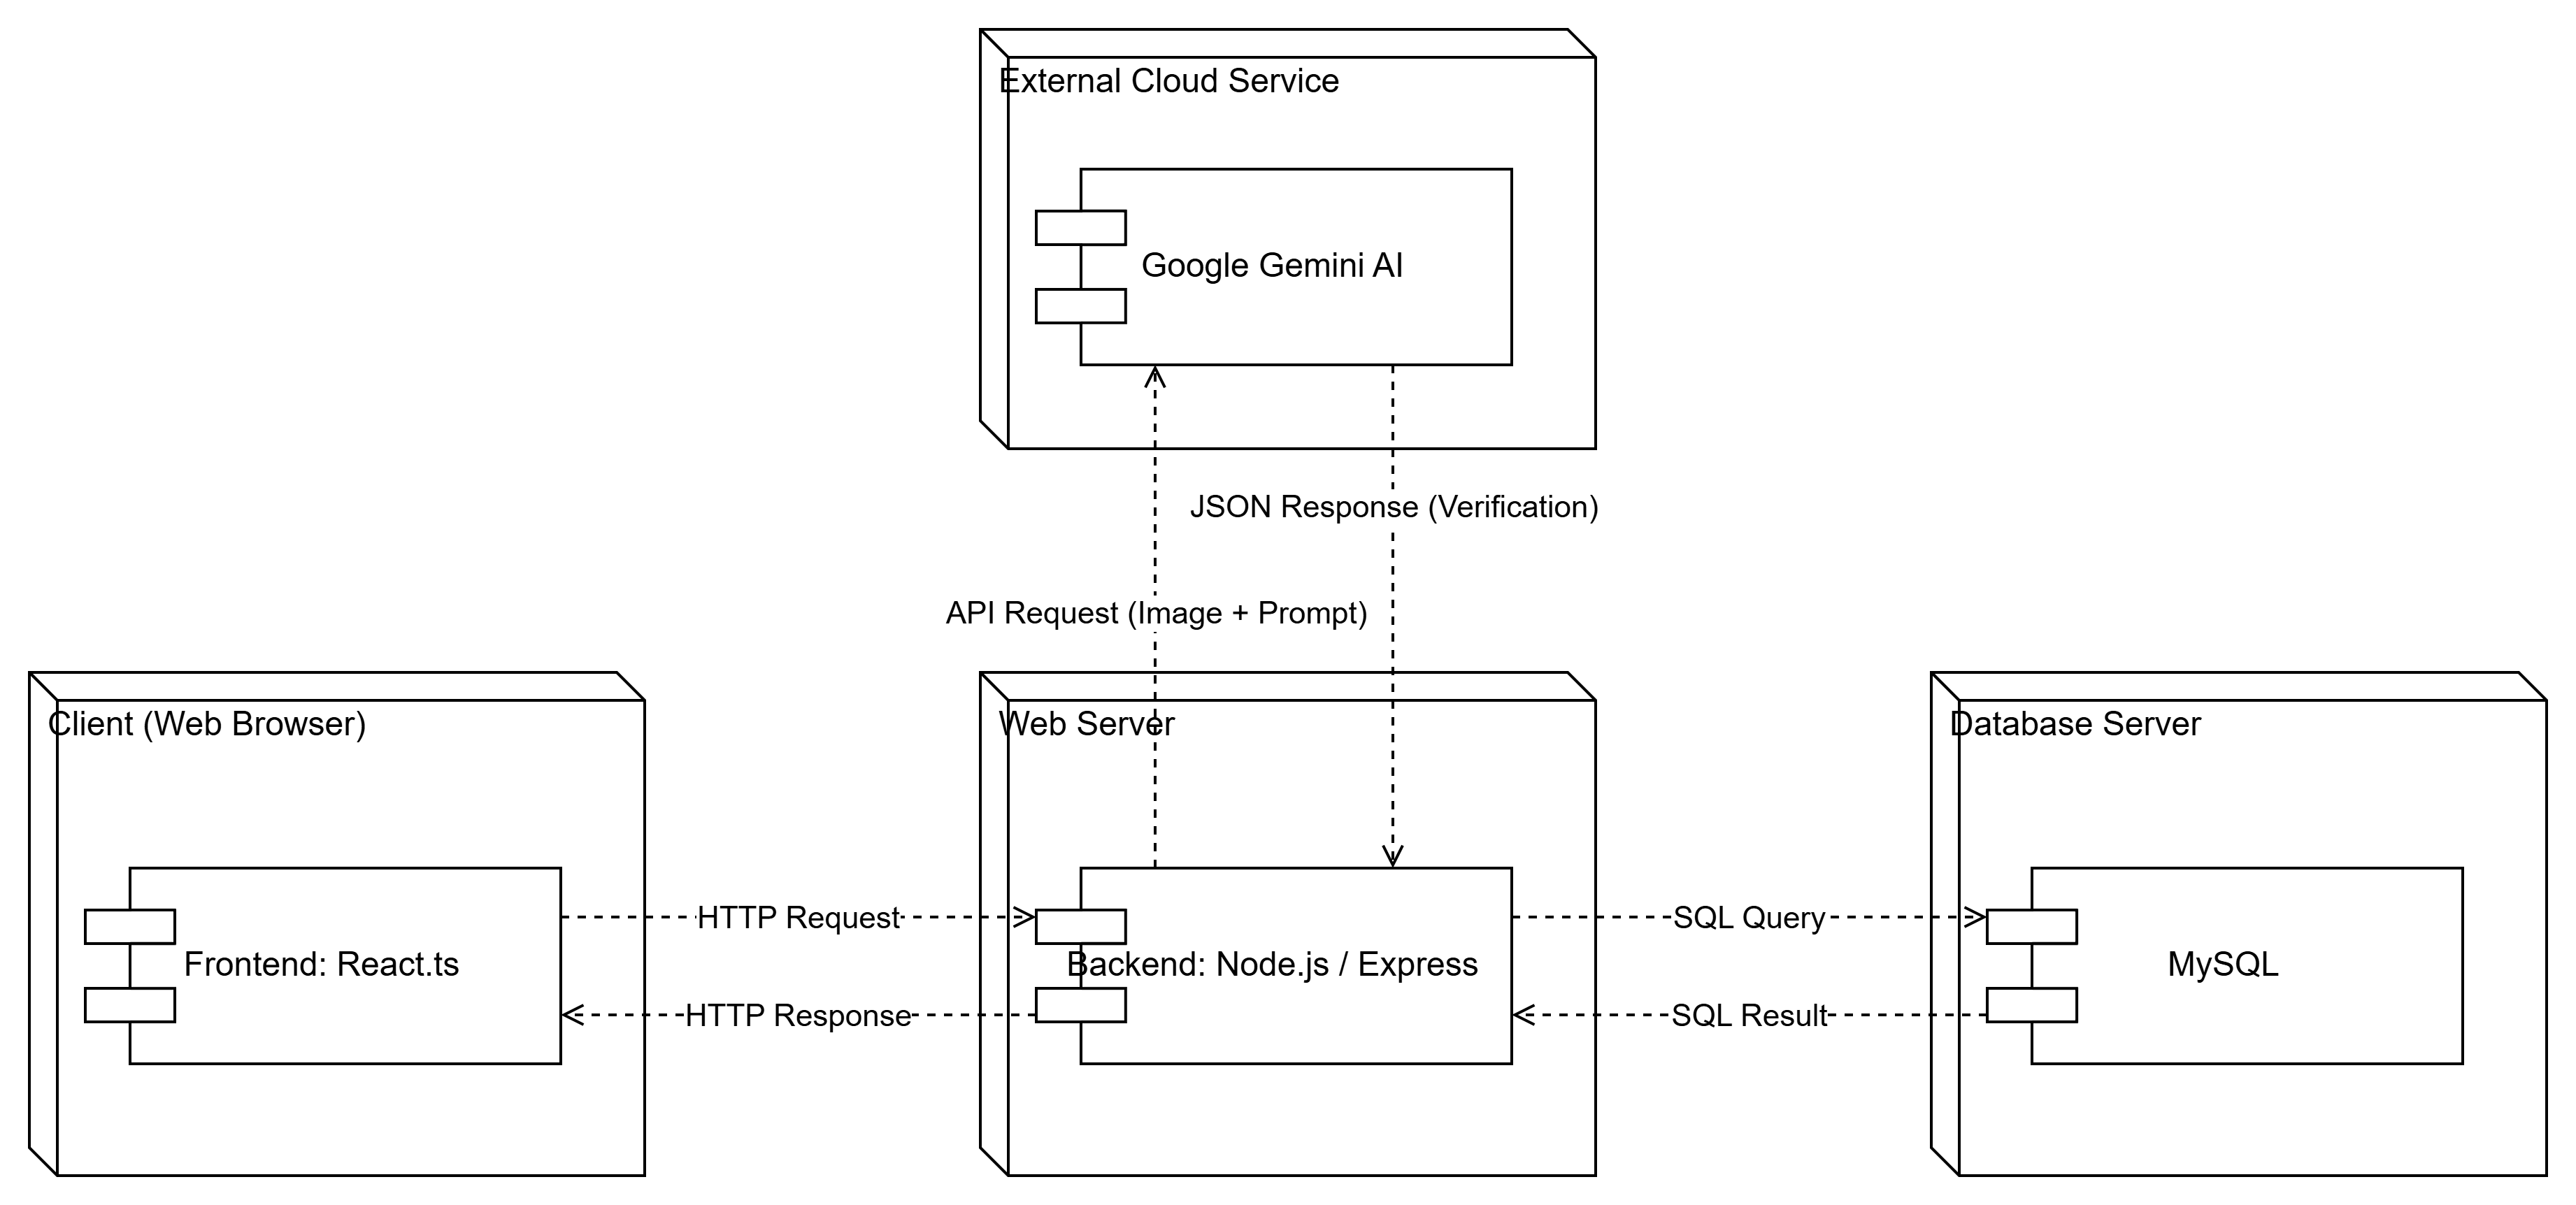
\includegraphics[width=1\textwidth]{image/bab3/Deployment Diagram Food AI Rescue.png}
    \caption{\textit{Deployment Diagram} Arsitektur Sistem Food AI Rescue}
    \label{fig:deployment-diagram}
\end{figure}

% ==============================================================================
\section{Pemodelan Sistem dan Data}
% ==============================================================================

Tahapan pemodelan sistem dan data bertujuan untuk memvisualisasikan alur interaksi aktor, struktur logika bisnis, dan organisasi penyimpanan informasi di dalam platform \textit{Food AI Rescue}. Rancang bangun ini direpresentasikan melalui serangkaian diagram analitis standar \textit{Unified Modeling Language} (UML) dan pemodelan relasional, yang meliputi \textit{Use Case Diagram} untuk memetakan batasan fungsional aktor, \textit{Entity Relationship Diagram} (ERD) untuk arsitektur pangkalan data, \textit{Class Diagram} untuk memetakan struktur objek pada peladen (\textit{server}), serta \textit{Sequence Diagram} untuk memvisualisasikan skenario pertukaran pesan dinamis pada fitur-fitur krusial.

% \subsection{\textit{Use Case Diagram}}
% \textit{Use Case Diagram} menggambarkan interaksi antara setiap aktor dengan fungsionalitas utama sistem Food AI Rescue. Terdapat 6 aktor utama yang berinteraksi dengan sistem, yaitu Donatur Individu, Donatur Korporat, Penerima, Relawan, Admin Pengelola, dan Super Admin.
%
% \begin{table}[H]
%     \centering
%     \caption{Deskripsi \textit{Use Case} Utama}
%     \label{tab:usecase}
%     \renewcommand{\arraystretch}{1.3}
%     \begin{tabular}{|p{2cm}|p{6cm}|p{6.5cm}|}
%         \hline
%         \textbf{Kode UC} & \textbf{Nama \textit{Use Case}} & \textbf{Aktor} \\
%         \hline
%         UC-01 & Unggah Donasi Makanan & Donatur Individu, Donatur Korporat \\
%         \hline
%         UC-02 & Verifikasi Kelayakan Makanan (AI) & Donatur Individu, Donatur Korporat \\
%         \hline
%         UC-03 & Klaim Donasi & Penerima \\
%         \hline
%         UC-04 & Pilih Metode Pengambilan & Penerima \\
%         \hline
%         UC-05 & Klaim Misi Pengantaran & Relawan \\
%         \hline
%         UC-06 & Pindai QR Code Serah Terima & Donatur, Relawan \\
%         \hline
%         UC-07 & Lihat Dasbor SROI & Donatur, Admin Pengelola \\
%         \hline
%         UC-08 & \textit{Generate} Konten AI Korporat & Donatur Korporat \\
%         \hline
%         UC-09 & Verifikasi Akun Pengguna & Admin Pengelola \\
%         \hline
%         UC-10 & Kelola \textit{Backend} Sistem & Super Admin \\
%         \hline
%     \end{tabular}
% \end{table}
%
% \noindent Berikut adalah narasi singkat untuk \textit{use case} inti sistem:
%
% \begin{description}
%     \item[UC-01 – Unggah Donasi Makanan:] Donatur mengunggah data makanan surplus meliputi foto, deskripsi, jumlah porsi, dan lokasi. Sebelum dipublikasikan, sistem mewajibkan donatur untuk menjalankan UC-02.
%     \item[UC-02 – Verifikasi Kelayakan Makanan (AI):] Donatur memindai foto makanan menggunakan kamera. Sistem mengirimkan gambar ke \textit{Google Gemini Vision API} untuk dianalisis kelayakan fisik, higienitas visual, dan kehalalannya. Hasil verifikasi ditampilkan secara instan.
%     \item[UC-06 – Pindai QR Code Serah Terima:] Merupakan \textit{use case} kritis untuk mencegah klaim ganda. Pada metode \textit{pick-up}, Donatur memindai QR Code Penerima. Pada metode diantar, Donatur memindai QR Code Relawan, kemudian Relawan memindai QR Code Penerima.
%     \item[UC-08 – Generate Konten AI Korporat:] Eksklusif untuk Donatur Korporat. Mencakup fitur \textit{Eco Packaging Editor} untuk menghasilkan desain kemasan ramah lingkungan dan \textit{CSR Copywriter} untuk menghasilkan konten promosi media sosial secara otomatis.
% \end{description}

\subsection{\textit{Use Case}}

\subsection{\textit{Entity Relationship Diagram} (ERD)}
ERD berikut menggambarkan struktur basis data relasional yang menjadi fondasi penyimpanan data platform Food AI Rescue. Entitas utama dan relasinya dijabarkan sebagai berikut:

\begin{longtable}{|p{4.5cm}|p{6cm}|p{4cm}|}
    \caption{Daftar Seluruh Entitas Basis Data Food AI Rescue}
    \label{tab:erd-entities-full} \\
    \hline
    \textbf{Entitas} & \textbf{Atribut Utama} & \textbf{Keterangan} \\
    \hline
    \endfirsthead
    \hline
    \textbf{Entitas} & \textbf{Atribut Utama} & \textbf{Keterangan} \\
    \hline
    \endhead
    \hline
    \multicolumn{3}{r}{\textit{Bersambung ke halaman berikutnya}} \\
    \endfoot
    \hline
    \endlastfoot
    \tbltt{addresses} & id, user\_id, label, full\_address, latitude, longitude, is\_primary & Titik lokasi dan alamat pengguna \\
    \hline
    \tbltt{admin\_targets} & id, metric\_key, target\_value, label & Konfigurasi target metrik admin \\
    \hline
    \tbltt{ai\_verifications} & id, food\_id, is\_edible, halal\_score, quality\_score, reason, allergens & Log hasil verifikasi kelayakan oleh AI \\
    \hline
    \tbltt{badges} & id, name, role, min\_points, icon, description & Sistem lencana untuk gamifikasi \\
    \hline
    \tbltt{broadcasts} & id, title, content, target, type, author\_id & Pengumuman atau siaran sistem \\
    \hline
    \tbltt{broadcast\_reads} & user\_id, broadcast\_id, read\_at & Status keterbacaan pengumuman \\
    \hline
    \tbltt{claims} & id, food\_id, receiver\_id, volunteer\_id, claimed\_quantity, status & Data transaksi klaim dan pengantaran \\
    \hline
    \tbltt{corporate\_ai\_generations} & id, donor\_id, food\_id, type, title, content & Data hasil AI generatif untuk korporat \\
    \hline
    \tbltt{email\_verifications} & id, email, code, expires\_at & Data kode verifikasi email \\
    \hline
    \tbltt{faqs} & id, category, question, answer & Pertanyaan yang sering diajukan \\
    \hline
    \tbltt{food\_items} & id, provider\_id, name, current\_quantity, category, status & Data pasokan dan donasi makanan \\
    \hline
    \tbltt{food\_requests} & id, receiver\_id, title, description, needed\_quantity, status & Permintaan spesifik donasi makanan \\
    \hline
    \tbltt{leaderboard\_snapshots} & id, user\_id, points, rank, period, snapshot\_date & Rekaman riwayat peringkat pengguna \\
    \hline
    \tbltt{notifications} & id, user\_id, type, title, message, is\_read & Sistem notifikasi pengguna \\
    \hline
    \tbltt{password\_resets} & id, user\_id, token, expires\_at & Token untuk pemulihan kata sandi \\
    \hline
    \tbltt{point\_histories} & id, user\_id, amount, activity\_type, reference\_id & Riwayat perolehan poin gamifikasi \\
    \hline
    \tbltt{quests} & id, title, description, target\_value, reward\_points & Daftar misi harian/spesifik gamifikasi \\
    \hline
    \tbltt{rank\_levels} & id, role, name, min\_points, benefits, color & Tingkatan level (pangkat) pengguna \\
    \hline
    \tbltt{reports} & id, reporter\_id, claim\_id, category, status, is\_urgent & Laporan aduan atau kendala donasi \\
    \hline
    \tbltt{reviews} & id, claim\_id, user\_id, partner\_id, food\_id, rating & Ulasan dan penilaian pasca-donasi \\
    \hline
    \tbltt{social\_impacts} & id, food\_id, co2\_per\_portion, water\_saved\_liter, land\_saved\_sqm & Metrik kalkulasi dampak sosial lingkungan \\
    \hline
    \tbltt{system\_logs} & id, actor\_id, actor\_name, action, severity & Catatan aktivitas di dalam sistem \\
    \hline
    \tbltt{system\_settings} & setting\_key, setting\_value, updated\_at & Pengaturan dinamis platform \\
    \hline
    \tbltt{users} & id, name, email, password, role, status, points, avatar & Data profil utama seluruh pengguna \\
    \hline
    \tbltt{user\_ai\_keys} & id, user\_id, api\_key, label & Kunci API pribadi milik pengguna \\
    \hline
    \tbltt{user\_impact\_stats} & user\_id, total\_waste\_kg, total\_co2\_kg, total\_water\_liter & Akumulasi total dampak tiap pengguna \\
    \hline
    \tbltt{user\_quests} & id, user\_id, quest\_id, current\_value, is\_completed & Progres pengerjaan misi pengguna \\
    \hline
    \tbltt{verification\_codes} & id, identifier, channel, email, code, type, expires\_at & Kode OTP multi-saluran \\
    \hline
\end{longtable}

\newpage
\begin{landscape}
    \centering
    \vfill
    \includegraphics[width=\linewidth, height=0.85\textheight, keepaspectratio]{image/bab3/erd.png}
    \captionsetup{hypcap=false}
    \captionof{figure}{Entity Relationship Diagram (ERD) Food AI Rescue}
    \label{fig:erd}
    \vfill
\end{landscape}

\newpage

\noindent Relasi antar entitas utama adalah sebagai berikut:
\begin{itemize}
    \item Satu \texttt{users} (donatur) dapat memiliki banyak \texttt{donations} (relasi \textit{one-to-many}).
    \item Satu \texttt{donations} dapat memiliki banyak \texttt{claims}, namun hanya satu klaim yang berstatus aktif pada satu waktu untuk mencegah \textit{double-claim}.
    \item Satu \texttt{claims} memiliki tepat satu \texttt{deliveries} jika metode pengantaran yang dipilih adalah ``Diantar Relawan''.
    \item Setiap \texttt{donations} yang berhasil diselesaikan akan menghasilkan satu entri pada \texttt{sroi\_records}.
    \item Setiap \texttt{users} (relawan) memiliki satu entri pada \texttt{leaderboard} yang diperbarui setiap misi selesai.
\end{itemize}

\subsection{\textit{Class Diagram}}
\textit{Class Diagram} (Diagram Kelas) pada aplikasi \textit{Food AI Rescue} (FAR) dimodelkan menggunakan pendekatan \textit{Service-Oriented Architecture} (SOA) yang memisahkan antara entitas data (Model), layanan pemroses (\textit{Service}/\textit{Utility}), dan antarmuka pengguna (\textit{Component}). Pemisahan ini ditandai dengan penggunaan \textit{stereotype} (seperti \texttt{<<entity>>}, \texttt{<<service>>}, dan \texttt{<<component>>}) guna mengidentifikasi peran masing-masing kelas di dalam sistem.

Rincian spesifikasi kelas, deskripsi fungsi, beserta daftar atribut dan metode (operasi) yang menyertainya dijabarkan secara lengkap pada Tabel \ref{tab:class-diagram} berikut:

\begin{longtable}{|p{0.4cm}|p{2.8cm}|p{3.5cm}|p{3cm}|p{3.8cm}|}
    \caption{Spesifikasi dan Penjelasan \textit{Class Diagram}}
    \label{tab:class-diagram} \\
    \hline
    \textbf{No} & \textbf{Nama Kelas \& \textit{Stereotype}} & \textbf{Deskripsi / Fungsi} & \textbf{Atribut Utama} & \textbf{Operasi / Metode Utama} \\
    \hline
    \endfirsthead
    \hline
    \textbf{No} & \textbf{Nama Kelas \& \textit{Stereotype}} & \textbf{Deskripsi / Fungsi} & \textbf{Atribut Utama} & \textbf{Operasi / Metode Utama} \\
    \hline
    \endhead
    \hline
    \multicolumn{5}{r}{\textit{Bersambung ke halaman berikutnya}} \\
    \endfoot
    \hline
    \endlastfoot

    1 & \textbf{System Enums} \newline \texttt{<<enumeration>>} & Kumpulan tipe data statis konstan yang digunakan untuk membatasi nilai input (seperti jenis peran, status makanan, dan metode pengiriman) guna mencegah anomali data di seluruh sistem. & \tbltt{UserRole, FoodStatus, ClaimStatus, DeliveryMethod} & \textit{(Tidak memiliki operasi/metode, hanya berisi nilai konstan)} \\
    \hline

    2 & \textbf{UserData} \newline \texttt{<<entity>>} & Merepresentasikan model data profil pengguna terdaftar, termasuk penyimpanan kredensial, peran (\textit{role}), dan total poin kontribusi (SROI/XP). & \tbltt{id, name, email, role, status, points, phone, address, password} & \tbltt{authenticate(), updatePoints(), verifyOTP()} \\
    \hline

    3 & \textbf{FoodItem} \newline \texttt{<<entity>>} & Merepresentasikan model data inventaris makanan surplus dari donatur. Menyimpan data kuantitas, waktu kadaluarsa, hingga hasil JSON verifikasi AI dan kalkulasi dampak sosial. & \tbltt{id, providerId, name, currentQuantity, expiryTime, aiVerification, socialImpact} & \tbltt{deductStock(), checkExpiry(), updateStatus()} \\
    \hline

    4 & \textbf{ClaimHistoryItem} \newline \texttt{<<entity>>} & Merepresentasikan model log transaksi pesanan yang menghubungkan entitas Donatur, Penerima, dan Relawan. Menyimpan kode unik serah terima dan data ulasan. & \tbltt{id, foodId, receiverId, volunteerId, uniqueCode, status, rating, review} & \tbltt{generateQR(), assignVolunteer(), scanAndComplete()} \\
    \hline

    5 & \textbf{Address} \newline \texttt{<<entity>>} & Model data yang menyimpan detail koordinat geolokasi dan alamat fisik pengguna untuk keperluan pemetaan dan penjemputan logistik. & \tbltt{id, userId, label, fullAddress, lat, lng, contactPhone} & \textit{(Sebagai entitas data murni, dimanipulasi oleh layanan basis data)} \\
    \hline

    6 & \textbf{DatabaseService} \newline \texttt{<<service>>} & Modul \textit{backend} utama yang bertugas mengelola koneksi dan mengeksekusi kueri langsung ke basis data MySQL (proses CRUD transaksi). & \tbltt{API\_URL, headers} & \tbltt{registerUser(), loginUser(), addFoodItem(), processClaimTransaction(), getClaims()} \\
    \hline

    7 & \textbf{AIService} \newline \texttt{<<service>>} & Layanan integrasi sistem cerdas yang menangani komunikasi (API \textit{Call}) ke model \textit{Google Gemini} untuk validasi makanan dan \textit{Generate} CSR. & \tbltt{apiKeys, currentKeyIndex, model} & \tbltt{verifyFoodSafety(), generateCSRContent(), designPackaging(), rotateKey()} \\
    \hline

    8 & \textbf{FileService} \newline \texttt{<<service>>} & Modul pengelola media untuk menangani kompresi, penyimpanan (\textit{upload}), dan penghapusan berkas gambar/foto ke dalam direktori lokal server. & \tbltt{uploadPath, maxFileSize} & \tbltt{uploadImage(), optimizeImage(), deleteFile()} \\
    \hline

    9 & \textbf{GamificationService} \newline \texttt{<<utility>>} & Skrip utilitas (\textit{helper}) yang berisi logika kalkulasi untuk menghitung \textit{Experience Point} (XP), menentukan pangkat (\textit{rank}), dan memberikan lencana ke pengguna. & \tbltt{rankLevels, badges} & \tbltt{calculateXP(), evaluateRank(), awardBadge(), getLeaderboard()} \\
    \hline

    10 & \textbf{ExpiryChecker} \newline \texttt{<<utility>>} & Pekerja latar belakang (\textit{background job}) yang secara berkala memeriksa waktu dan mengubah status makanan jika telah melewati batas waktu aman konsumsi. & \textit{(Skrip berjalan independen tanpa atribut state tetap)} & \tbltt{checkAndExpireItems(), isFoodExpired()} \\
    \hline

    11 & \textbf{App} \newline \texttt{<<component>>} & Komponen akar (\textit{root}) dari \textit{Frontend} (React) yang bertindak sebagai \textit{router} utama pengelola sesi dan pengarah antarmuka ke dasbor masing-masing \textit{role}. & \tbltt{currentView, role, currentUser, isDarkMode} & \tbltt{handleLogin(), handleLogout(), handleClaimFood(), renderContent()} \\
    \hline

    12 & \textbf{ProviderIndex} \newline \texttt{<<component>>} & Komponen antarmuka pengguna untuk Donatur (Individu/Korporat). Mengelola UI inventaris, riwayat donasi, dan pemicu alat AI Korporat. & \tbltt{foodItems, claimHistory} & \tbltt{renderDashboard(), renderInventory(), renderOrders()} \\
    \hline

    13 & \textbf{ReceiverIndex} \newline \texttt{<<component>>} & Komponen antarmuka pengguna untuk Penerima. Mengelola UI katalog makanan yang tersedia dan formulir penyelesaian klaim/laporan. & \tbltt{availableFood, selectedFood} & \tbltt{renderFoodList(), renderFoodDetail(), handleClaim()} \\
    \hline

    14 & \textbf{VolunteerIndex} \newline \texttt{<<component>>} & Komponen antarmuka pengguna untuk Relawan. Mengelola UI papan misi (\textit{Missions Board}) geografis dan visualisasi \textit{leaderboard} gamifikasi. & \tbltt{missions, leaderboard} & \tbltt{renderMissions(), acceptMission(), renderLeaderboard()} \\
    \hline

    15 & \textbf{AdminIndex} \newline \texttt{<<component>>} & Komponen antarmuka pengguna panel kontrol untuk Administrator. Digunakan untuk memoderasi laporan sengketa dan memverifikasi pengguna baru. & \tbltt{users, reports, systemLogs} & \tbltt{renderCommunity(), renderModeration(), verifyUser()} \\
    \hline

\end{longtable}

\noindent Hubungan antar kelas yang penting:
\begin{itemize}
    \item \texttt{App} (\texttt{<<component>>}) bertindak sebagai orkestrator utama yang menginstansiasi \texttt{DatabaseService} dan \texttt{AIService} untuk seluruh operasi data dan AI.
    \item \texttt{FoodItem} berasosiasi dengan \texttt{AIService} melalui atribut \texttt{aiVerification} yang diisi setelah proses \texttt{verifyFoodSafety()} selesai.
    \item \texttt{ClaimHistoryItem} berasosiasi dengan \texttt{GamificationService} — setiap kali \texttt{scanAndComplete()} dipanggil, sistem memicu \texttt{calculateXP()} dan \texttt{evaluateRank()}.
    \item \texttt{ExpiryChecker} memantau seluruh entitas \texttt{FoodItem} secara periodik dan memanggil \texttt{updateStatus()} jika makanan telah melewati \texttt{expiryTime}.
    \item \texttt{FileService} digunakan oleh \texttt{DatabaseService} setiap kali ada operasi unggah foto makanan atau aset AI generatif.
\end{itemize}

\newpage
\begin{landscape}
    \centering
    \vfill
    \includesvg[width=\linewidth, height=0.85\textheight, keepaspectratio, inkscapelatex=false]{image/bab3/class diagram}
    \captionsetup{hypcap=false}
    \captionof{figure}{\textit{Class Diagram} Food AI Rescue}
    \label{fig:class-diagram}
    \vfill
\end{landscape}
\newpage

\subsection{\textit{Sequence Diagram}}
\textit{Sequence diagram} merupakan grafik dua dimensi di mana objek ditunjukkan pada dimensi horizontal, sedangkan garis waktu (\textit{lifeline}) ditunjukkan pada dimensi vertikal. Pada sistem Food AI Rescue, \textit{Sequence Diagram} digunakan untuk memvisualisasikan urutan interaksi antara pengguna (aktor) dan berbagai komponen sistem dalam mengeksekusi sebuah proses. Diagram ini menguraikan secara terperinci bagaimana aliran pesan (\textit{message}) dikirim dan diterima secara berurutan, dimulai dari interaksi pengguna pada antarmuka aplikasi (\textit{Client/Frontend}), pemrosesan permintaan oleh peladen (\textit{Backend API}), integrasi dengan layanan Kecerdasan Buatan (\textit{Google Gemini AI}), hingga proses penyimpanan dan pemberian respons oleh basis data (\textit{Database}).

Untuk memberikan gambaran teknis yang lebih komprehensif, berikut ini disajikan rincian \textit{sequence diagram} yang memetakan seluruh alur proses utama pada sistem Food AI Rescue.

% ------------------------------------------------------------------
\subsubsection{Alur Global (Umum)}
% ------------------------------------------------------------------

\textbf{1. \textit{Sequence Diagram} Melakukan \textit{Login} (Global)}

Pengguna memasukkan email dan kata sandi di Halaman \textit{Login}. Sistem mengirimkan perintah \texttt{validateLogin(email, password)} ke \textit{Auth Service}. Layanan ini kemudian melakukan kueri ke \textit{Database} untuk memverifikasi kredensial. Jika kredensial salah, \textit{Database} menyatakan data tidak ditemukan dan pesan \textit{error} ditampilkan ke pengguna. Jika benar, sistem melakukan \textit{Generate JWT Token \& Session}, mengirimkan token kesuksesan, dan me-\textit{redirect} pengguna ke \textit{Dashboard Role} masing-masing secara spesifik.

\begin{figure}[H]
    \centering
    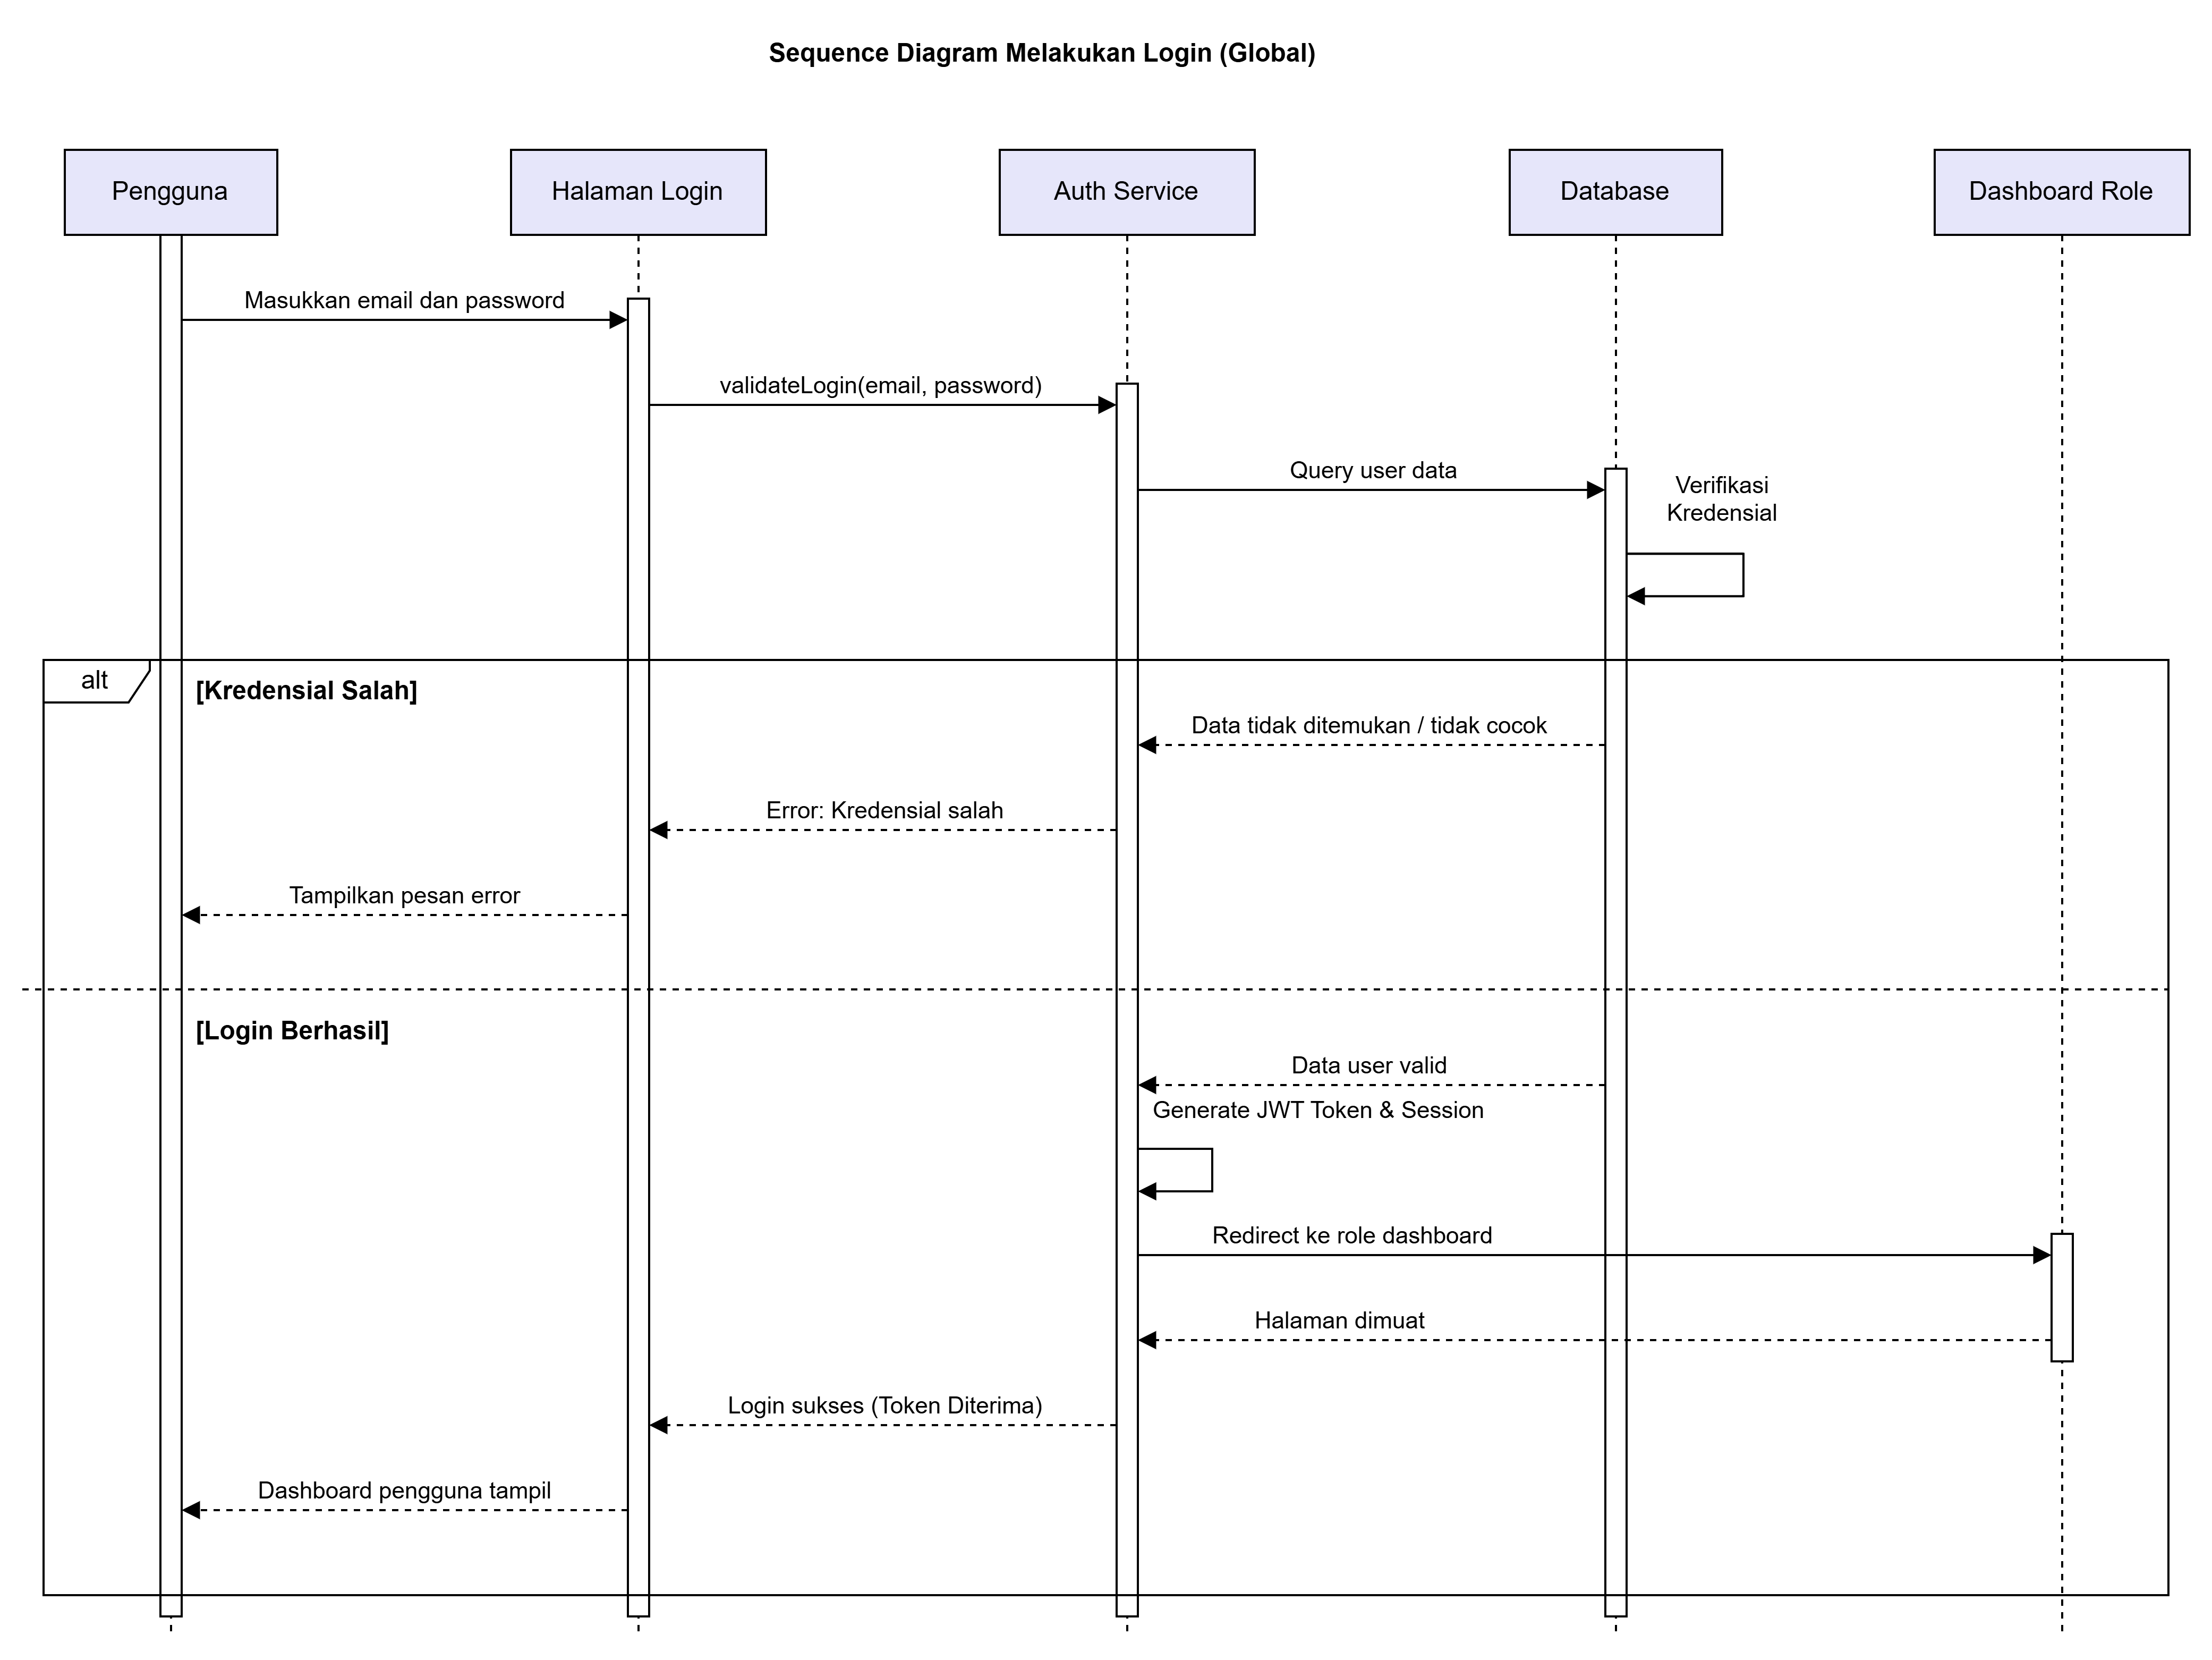
\includegraphics[width=1\textwidth]{image/bab3/sequence/Sequence Diagram Melakukan Login (Global).png}
    \captionsetup{hypcap=false}
    \caption{\textit{Sequence Diagram} Melakukan \textit{Login} (Global)}
    \label{fig:sd-login}
\end{figure}

% ------------------------------------------------------------------
\subsubsection{Alur Donatur (Individu \& Korporat)}
% ------------------------------------------------------------------

\textbf{2. \textit{Sequence Diagram} Unggah Surplus Makanan \& Verifikasi AI}

Donatur mengisi data makanan dan mengunggah fotonya melalui \textit{Form Upload}. Sistem mengirim data tersebut (\texttt{verifyFoodData}) ke \textit{Backend API}. \textit{Backend} kemudian mengirimkan instruksi teks (\textit{prompt}) beserta foto ke layanan \textbf{Google Gemini API}. Gemini merespons dengan JSON berisi skor keamanan, daftar bahan, alergen, dan skor sosial. Hasil ini ditampilkan ke donatur. Jika donatur menekan ``Publikasikan'', fungsi \texttt{publishFoodItem} dipanggil, data disimpan ke \textit{Database}, dan status makanan berubah menjadi \textit{AVAILABLE}.

\begin{figure}[H]
    \centering
    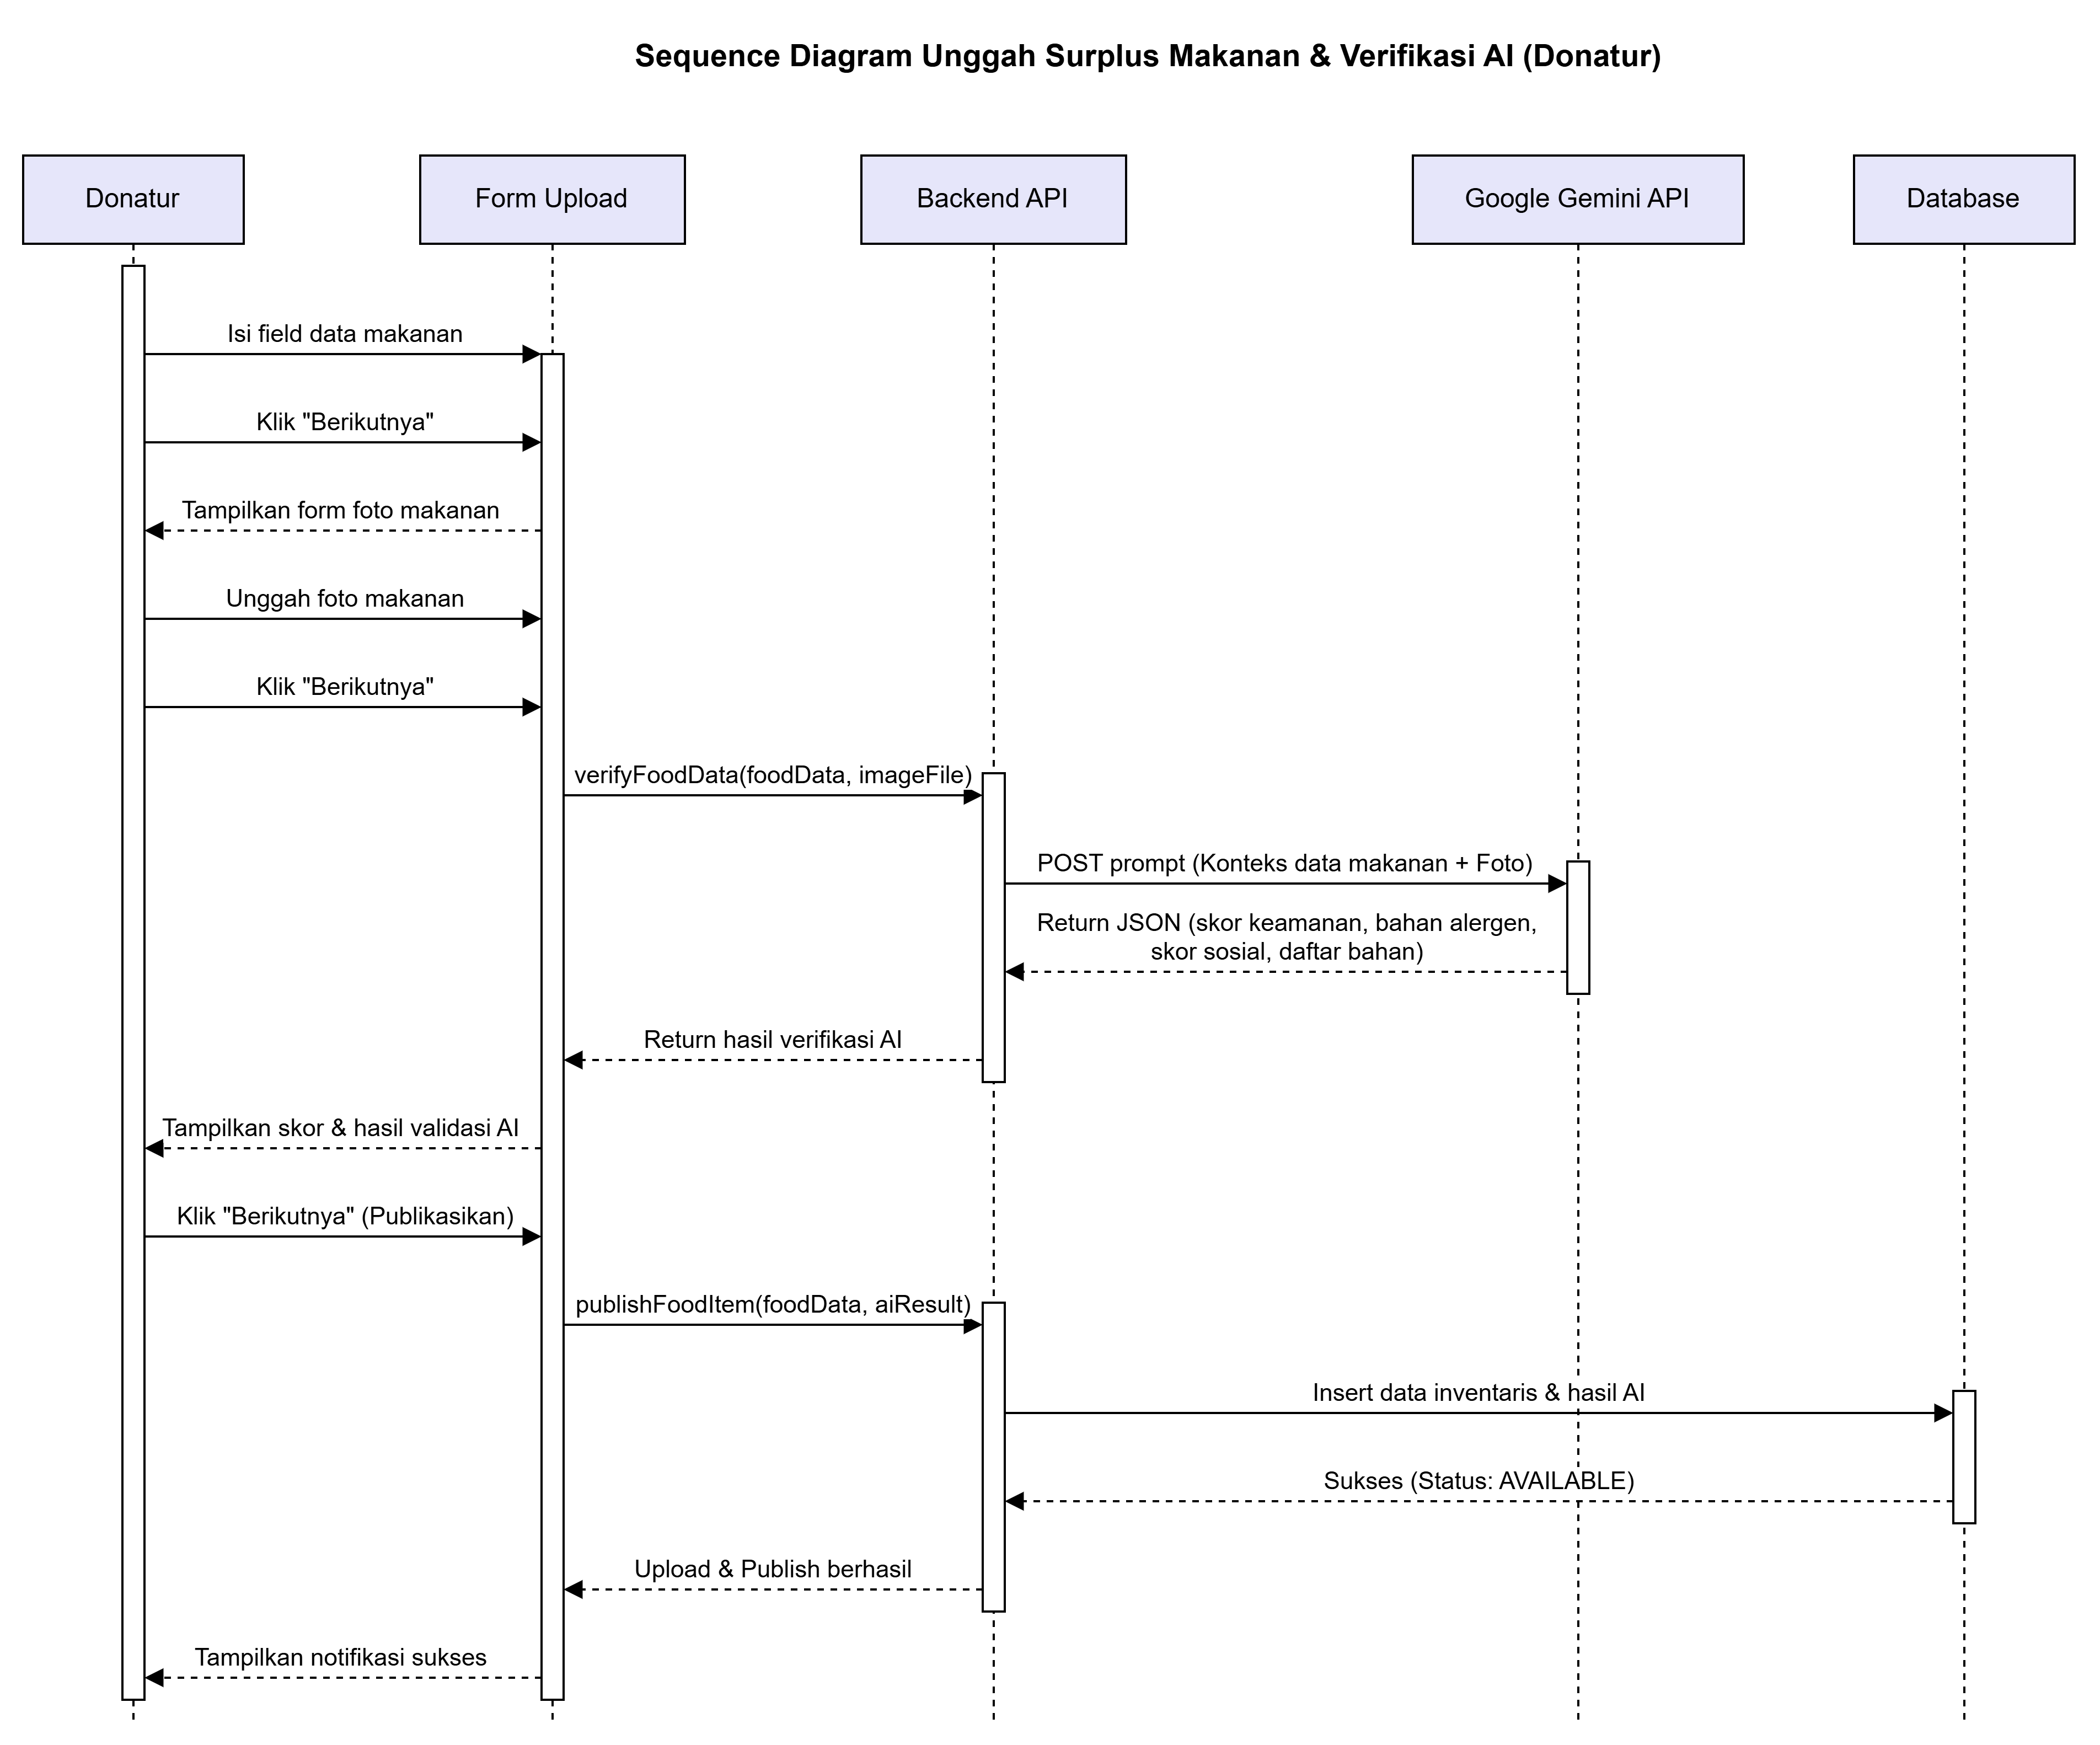
\includegraphics[width=1\textwidth]{image/bab3/sequence/Sequence Diagram Unggah Surplus Makanan & Verifikasi AI (Donatur).png}
    \captionsetup{hypcap=false}
    \caption{\textit{Sequence Diagram} Unggah Surplus Makanan \& Verifikasi AI (Donatur)}
    \label{fig:sd-upload-donatur}
\end{figure}

\textbf{3. \textit{Sequence Diagram} Konfirmasi Pesanan}

Donatur melihat daftar pesanan yang masuk dan mengklik ``Terima''. \textit{Dashboard} mengirim perintah \texttt{handleApproveClaim(claimId)} ke \textit{Backend}. \textit{Backend} memperbarui status klaim menjadi \textit{APPROVED/READY} di \textit{Database}, lalu mengirimkan notifikasi ke Penerima atau Relawan bahwa pesanan ``Siap Diambil''.

\begin{figure}[H]
    \centering
    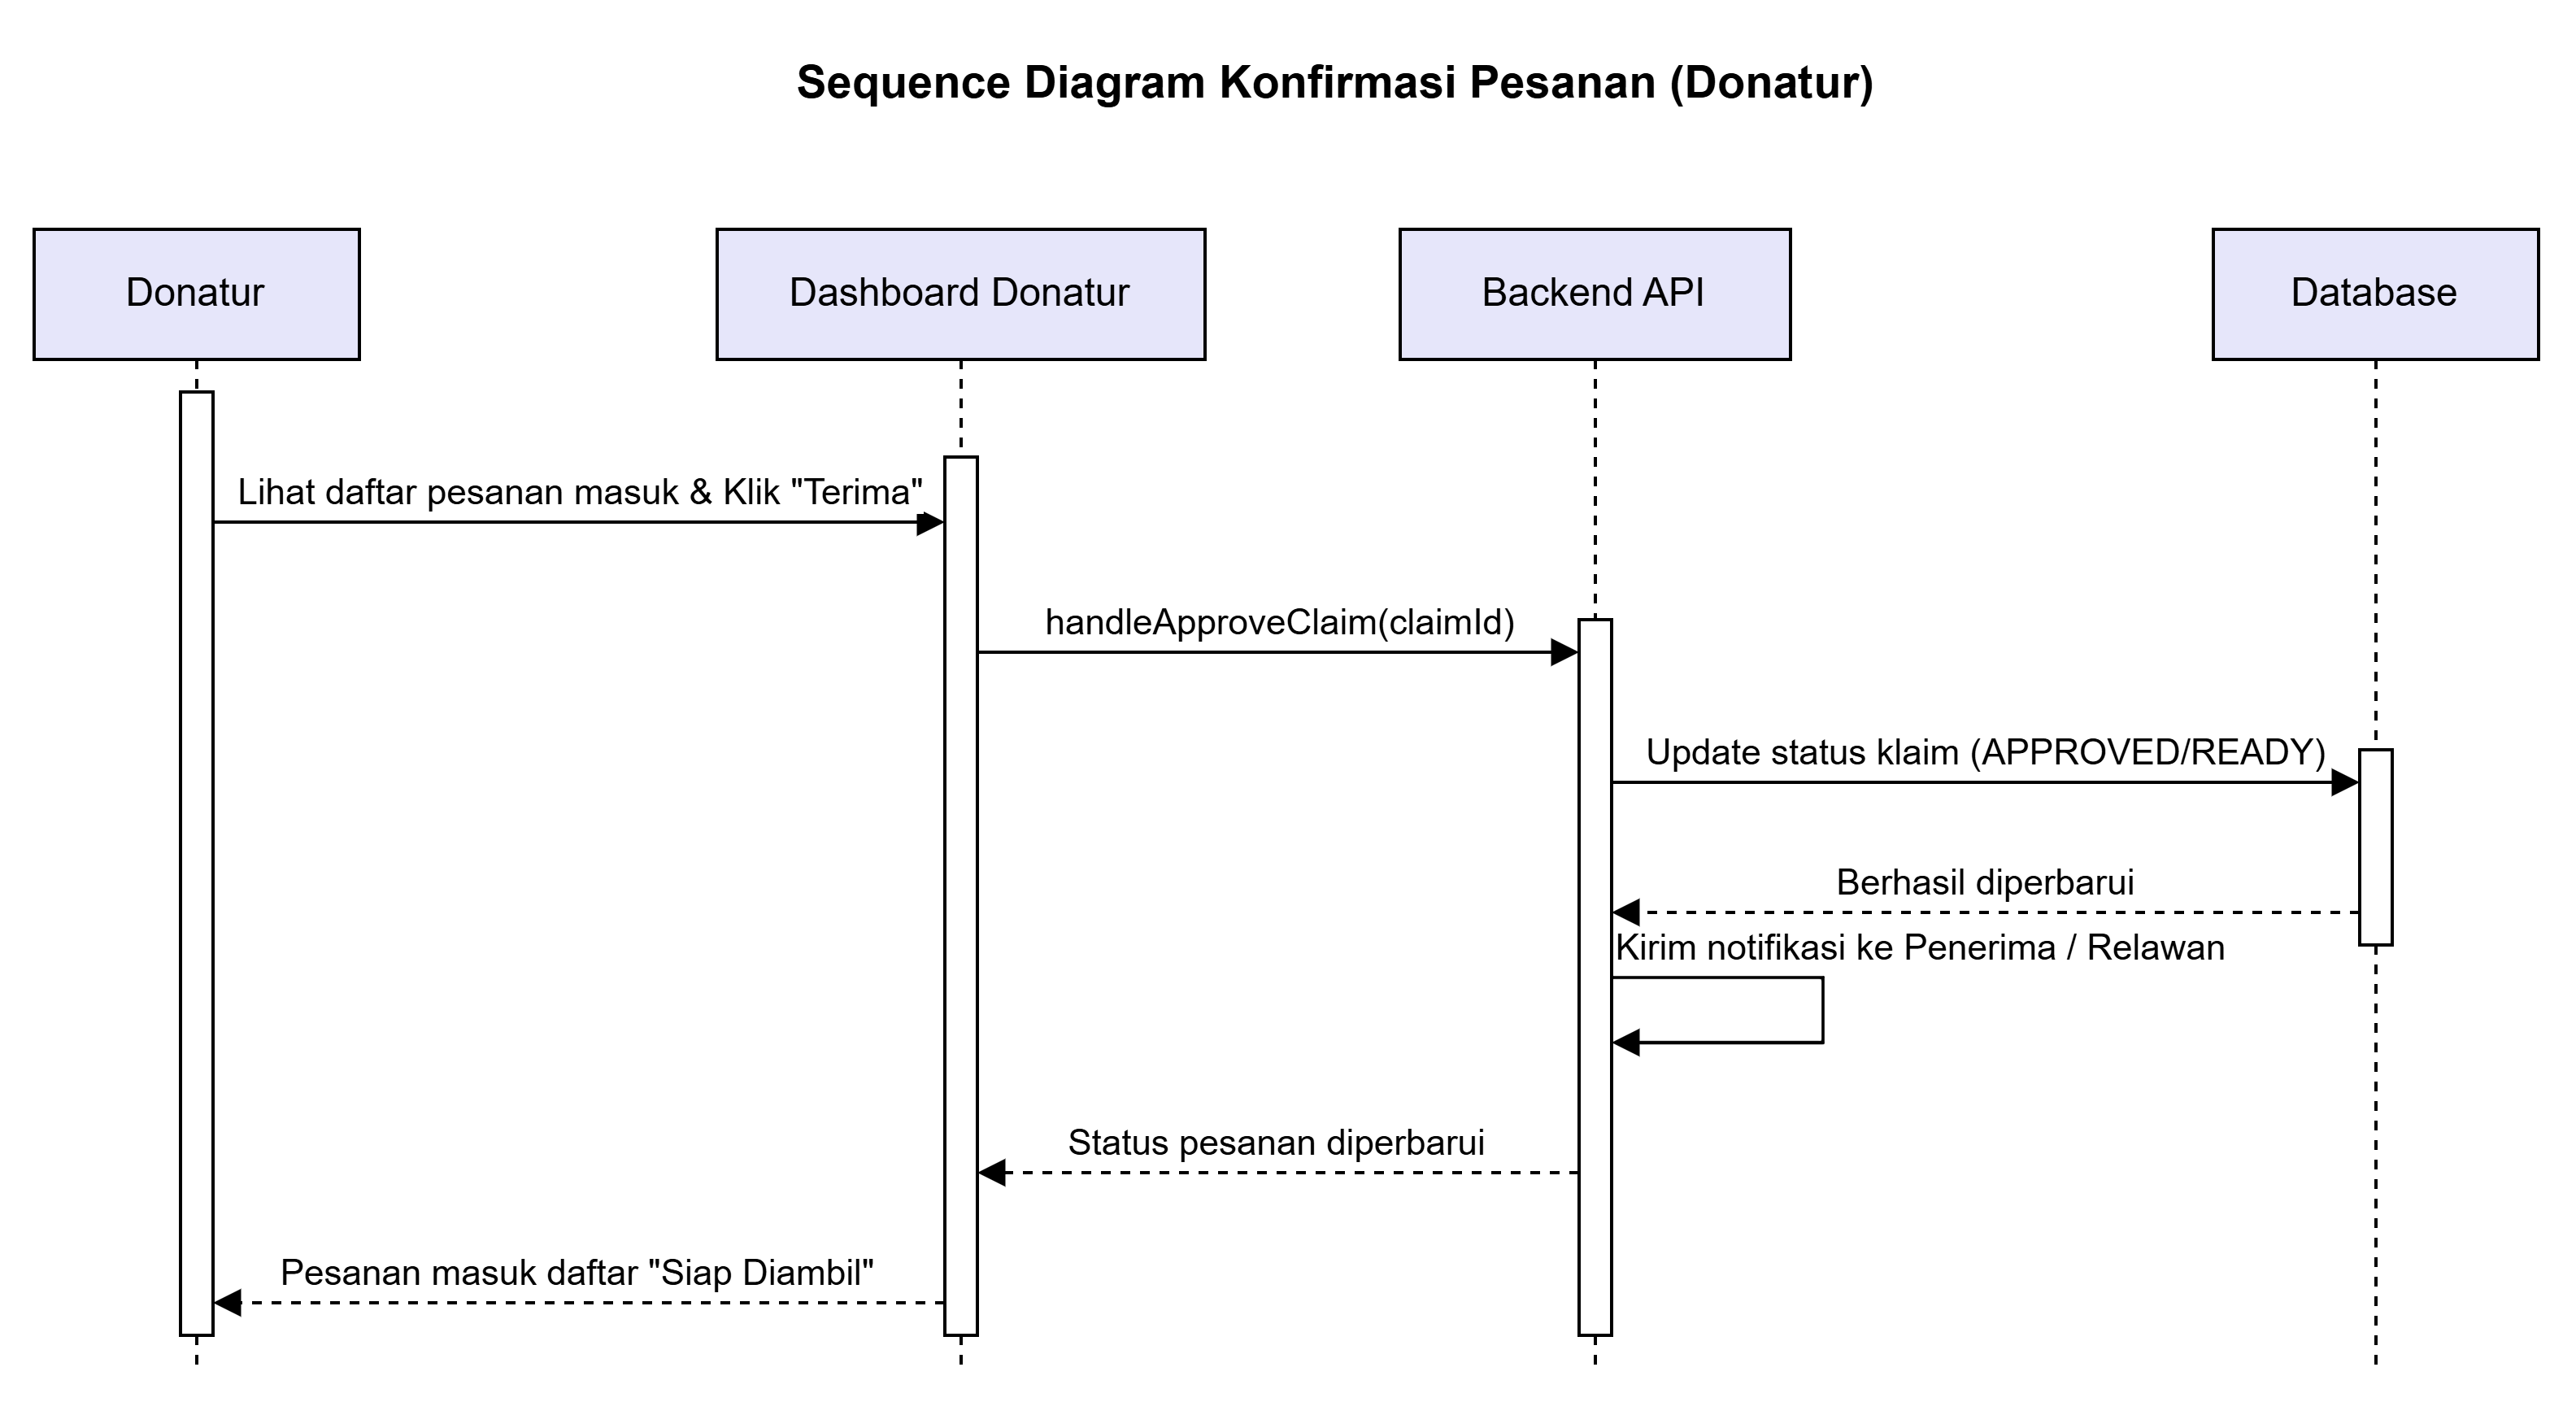
\includegraphics[width=1\textwidth]{image/bab3/sequence/Sequence Diagram Konfirmasi Pesanan (Donatur).png}
    \captionsetup{hypcap=false}
    \caption{\textit{Sequence Diagram} Konfirmasi Pesanan (Donatur)}
    \label{fig:sd-konfirmasi-donatur}
\end{figure}

\textbf{4. \textit{Sequence Diagram} Dasbor Dampak Sosial SROI \& Jejak Karbon}

Donatur membuka halaman Dampak Sosial. Antarmuka memanggil \texttt{fetchImpactStats(userId)} ke \textit{Backend}. \textit{Backend} melakukan agregasi kalkulasi pencegahan limbah (\texttt{waste\_kg}) dan karbon (\texttt{co2\_kg}) dari \textit{Database}. Hasil statistik dikembalikan dalam format JSON untuk dirender menjadi grafik CO\textsubscript{2} yang interaktif pada antarmuka pengguna.

\begin{figure}[H]
    \centering
    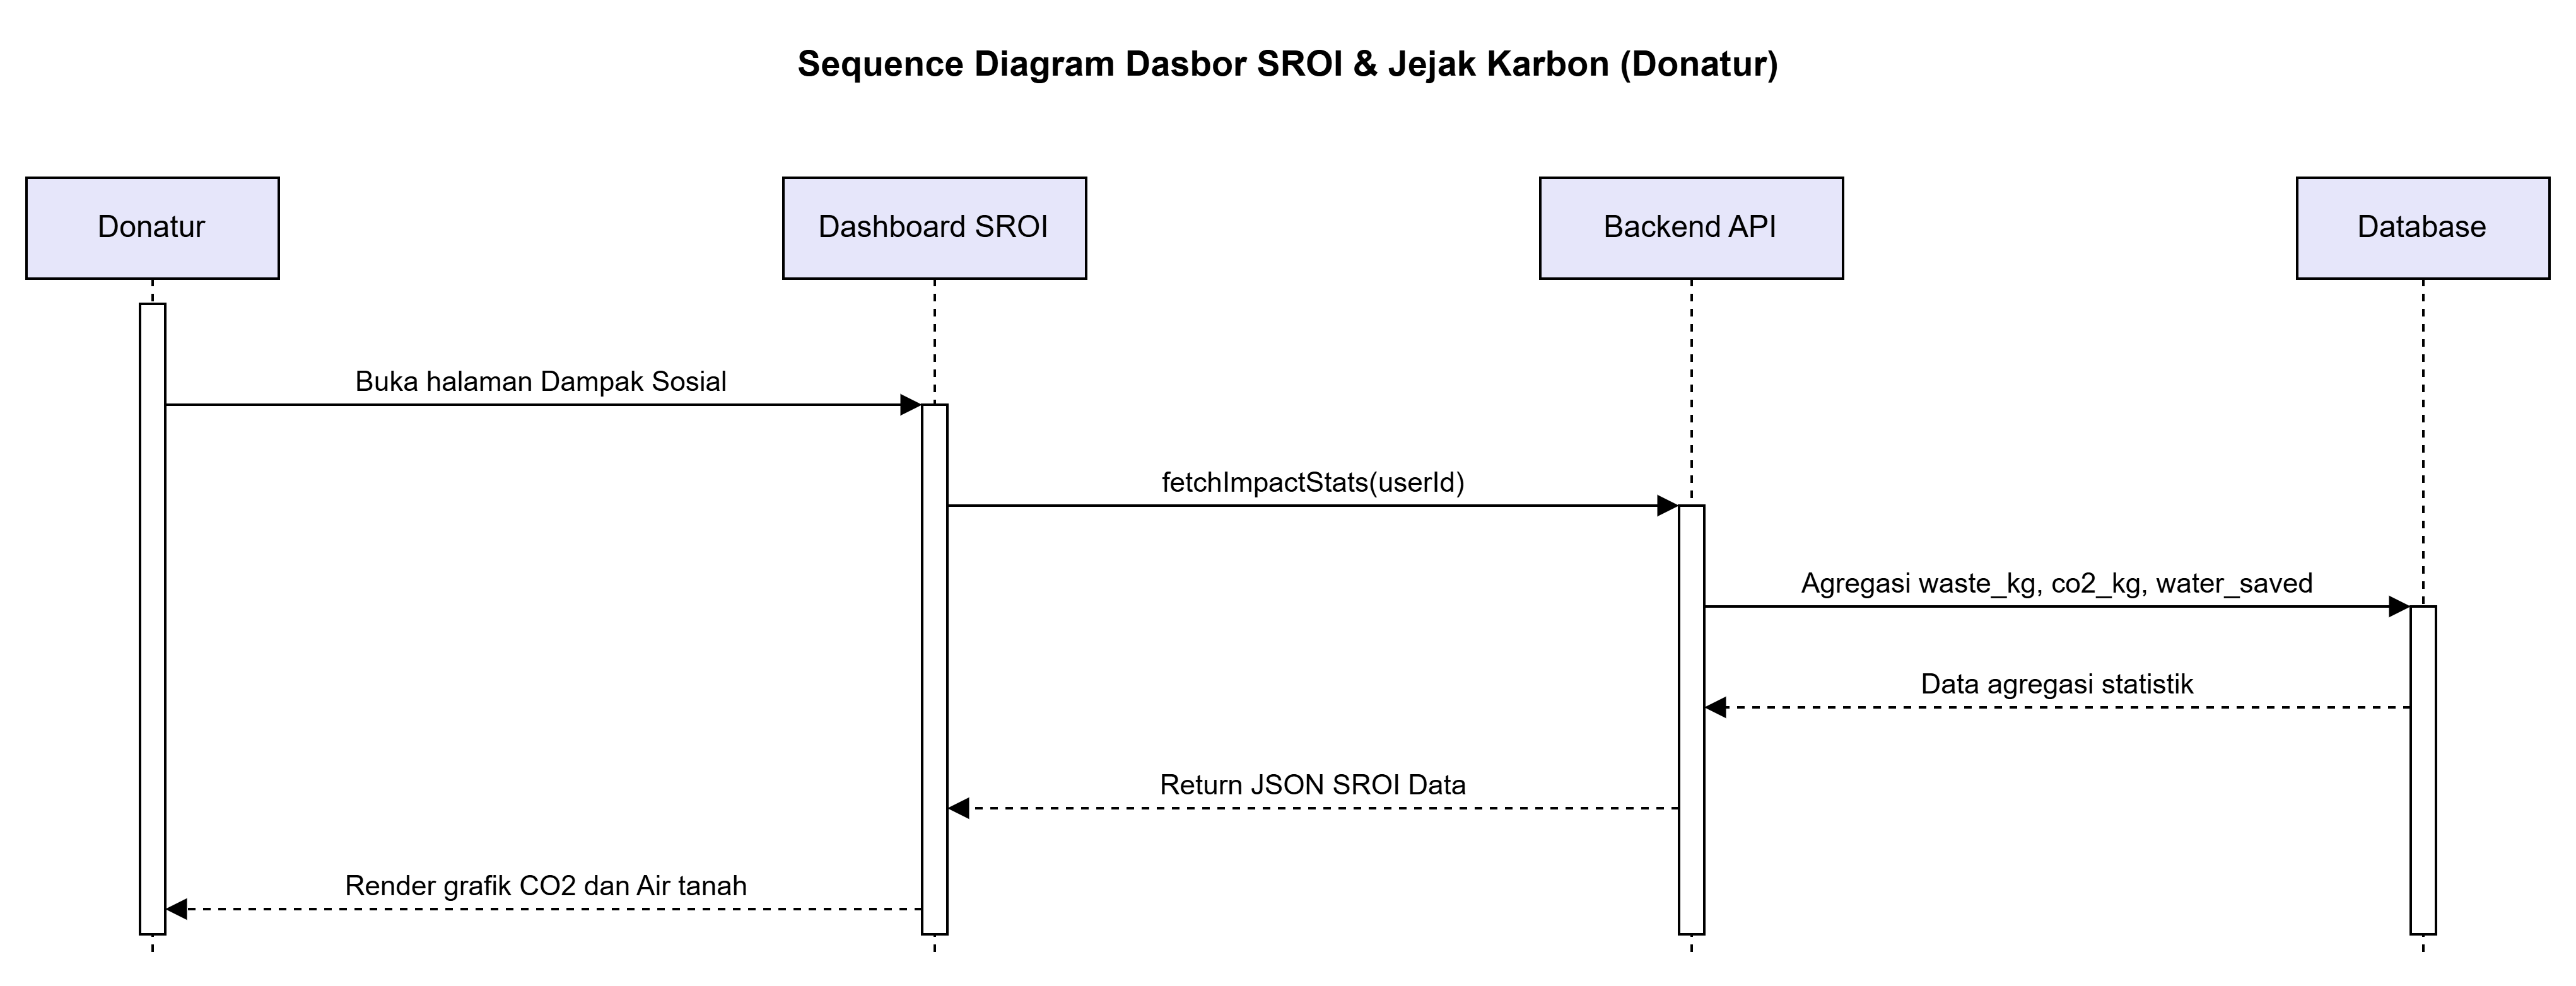
\includegraphics[width=1\textwidth]{image/bab3/sequence/Sequence Diagram Dasbor Dampak Sosial SROI (Donatur).png}
    \captionsetup{hypcap=false}
    \caption{\textit{Sequence Diagram} Dasbor Dampak Sosial SROI (Donatur)}
    \label{fig:sd-sroi-donatur}
\end{figure}

% ------------------------------------------------------------------
\subsubsection{Alur Eksklusif Donatur Korporat (AI Generatif)}
% ------------------------------------------------------------------

\textbf{5. \textit{Sequence Diagram} Pembuatan Logo \& Rekomendasi Kemasan}

Donatur Korporat memasukkan daftar makanan dan instruksi logo di \textit{Packaging Studio}. Studio memanggil \texttt{generatePackagingSolution} ke \textit{AI Service}. AI kemudian mengirim \textit{POST prompt image} ke Gemini API untuk membuat logo, dan \textit{POST prompt text} untuk mencari rekomendasi material ramah lingkungan. URL gambar dan teks rekomendasi dikembalikan untuk ditampilkan ke pengguna.

\begin{figure}[H]
    \centering
    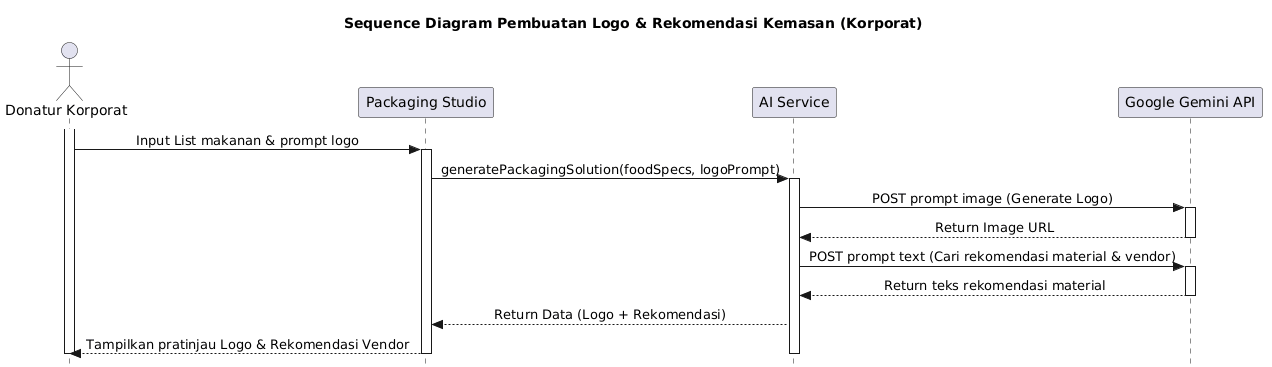
\includegraphics[width=1\textwidth]{image/bab3/sequence/Sequence Diagram Pembuatan Logo & Rekomendasi Kemasan (Korporat).png}
    \captionsetup{hypcap=false}
    \caption{\textit{Sequence Diagram} Pembuatan Logo \& Rekomendasi Kemasan (Donatur Korporat)}
    \label{fig:sd-kemasan-korporat}
\end{figure}

\textbf{6. \textit{Sequence Diagram} \textit{Generate} CSR \textit{Copywriter}}

Pengguna korporat memilih jenis makanan, nada bahasa (\textit{tone}), dan platform media sosial pada \textit{CSR Editor}. Sistem memanggil \textit{AI Service}, yang pertama-tama mengambil spesifikasi donasi dari \textit{Database}. AI kemudian mengirim instruksi ke Gemini API untuk membuat 2 versi takarir (\textit{caption}). Draf ini disimpan ke tabel \texttt{corporate\_ai\_generations} di \textit{database} sebelum ditampilkan ke pengguna.

\begin{figure}[H]
    \centering
    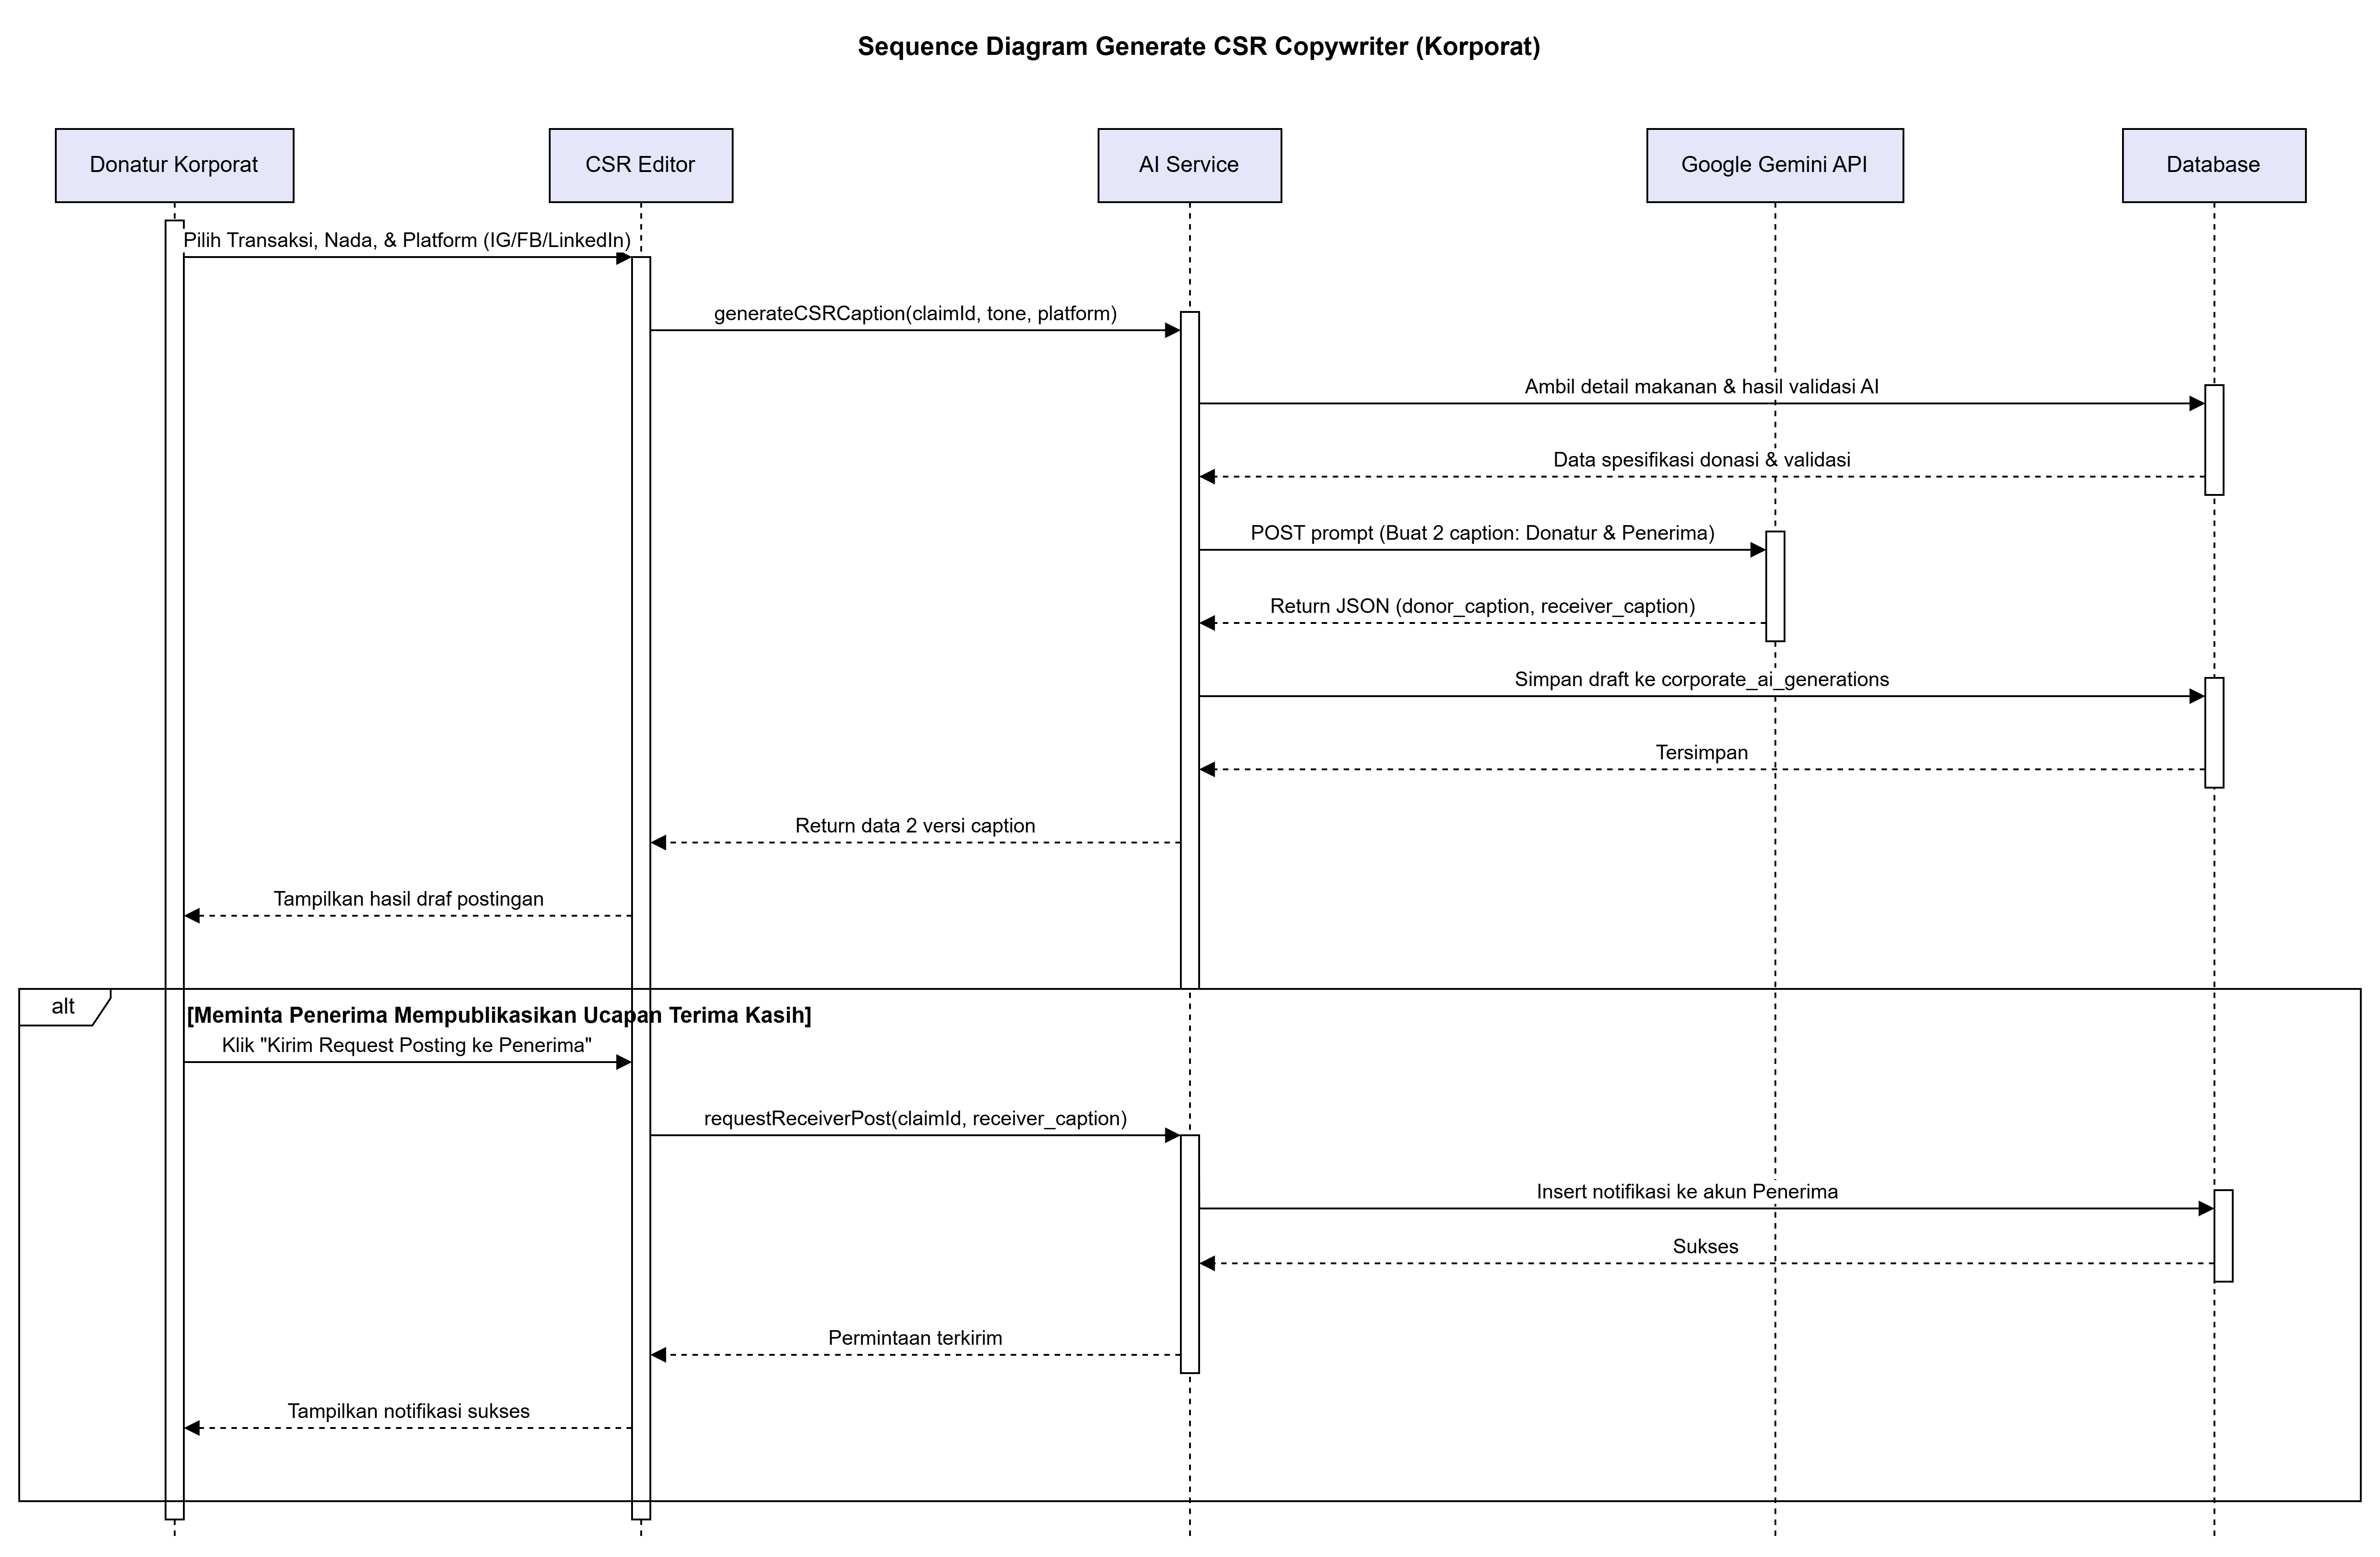
\includegraphics[width=1\textwidth]{image/bab3/sequence/Sequence Diagram Generate CSR Copywriter (Korporat).png}
    \captionsetup{hypcap=false}
    \caption{\textit{Sequence Diagram} \textit{Generate} CSR \textit{Copywriter} (Donatur Korporat)}
    \label{fig:sd-csr-korporat}
\end{figure}

% ------------------------------------------------------------------
\subsubsection{Alur Penerima Donasi}
% ------------------------------------------------------------------

\textbf{7. \textit{Sequence Diagram} Pencarian \& Klaim Makanan}

Penerima memilih makanan dan metode pengambilan, lalu mengklik ``Klaim''. \textit{Backend} menerima \texttt{handleClaimFood} dan mengecek ketersediaan stok di \textit{Database}. Jika stok habis, proses digagalkan. Jika tersedia, \textit{Backend} akan men-\textit{generate Unique Code} (Kode QR), melakukan kalkulasi dampak, mengurangi stok di \textit{database}, dan menyimpan klaim baru. Antarmuka kemudian menampilkan \textit{Success Splash Screen}.

\begin{figure}[H]
    \centering
    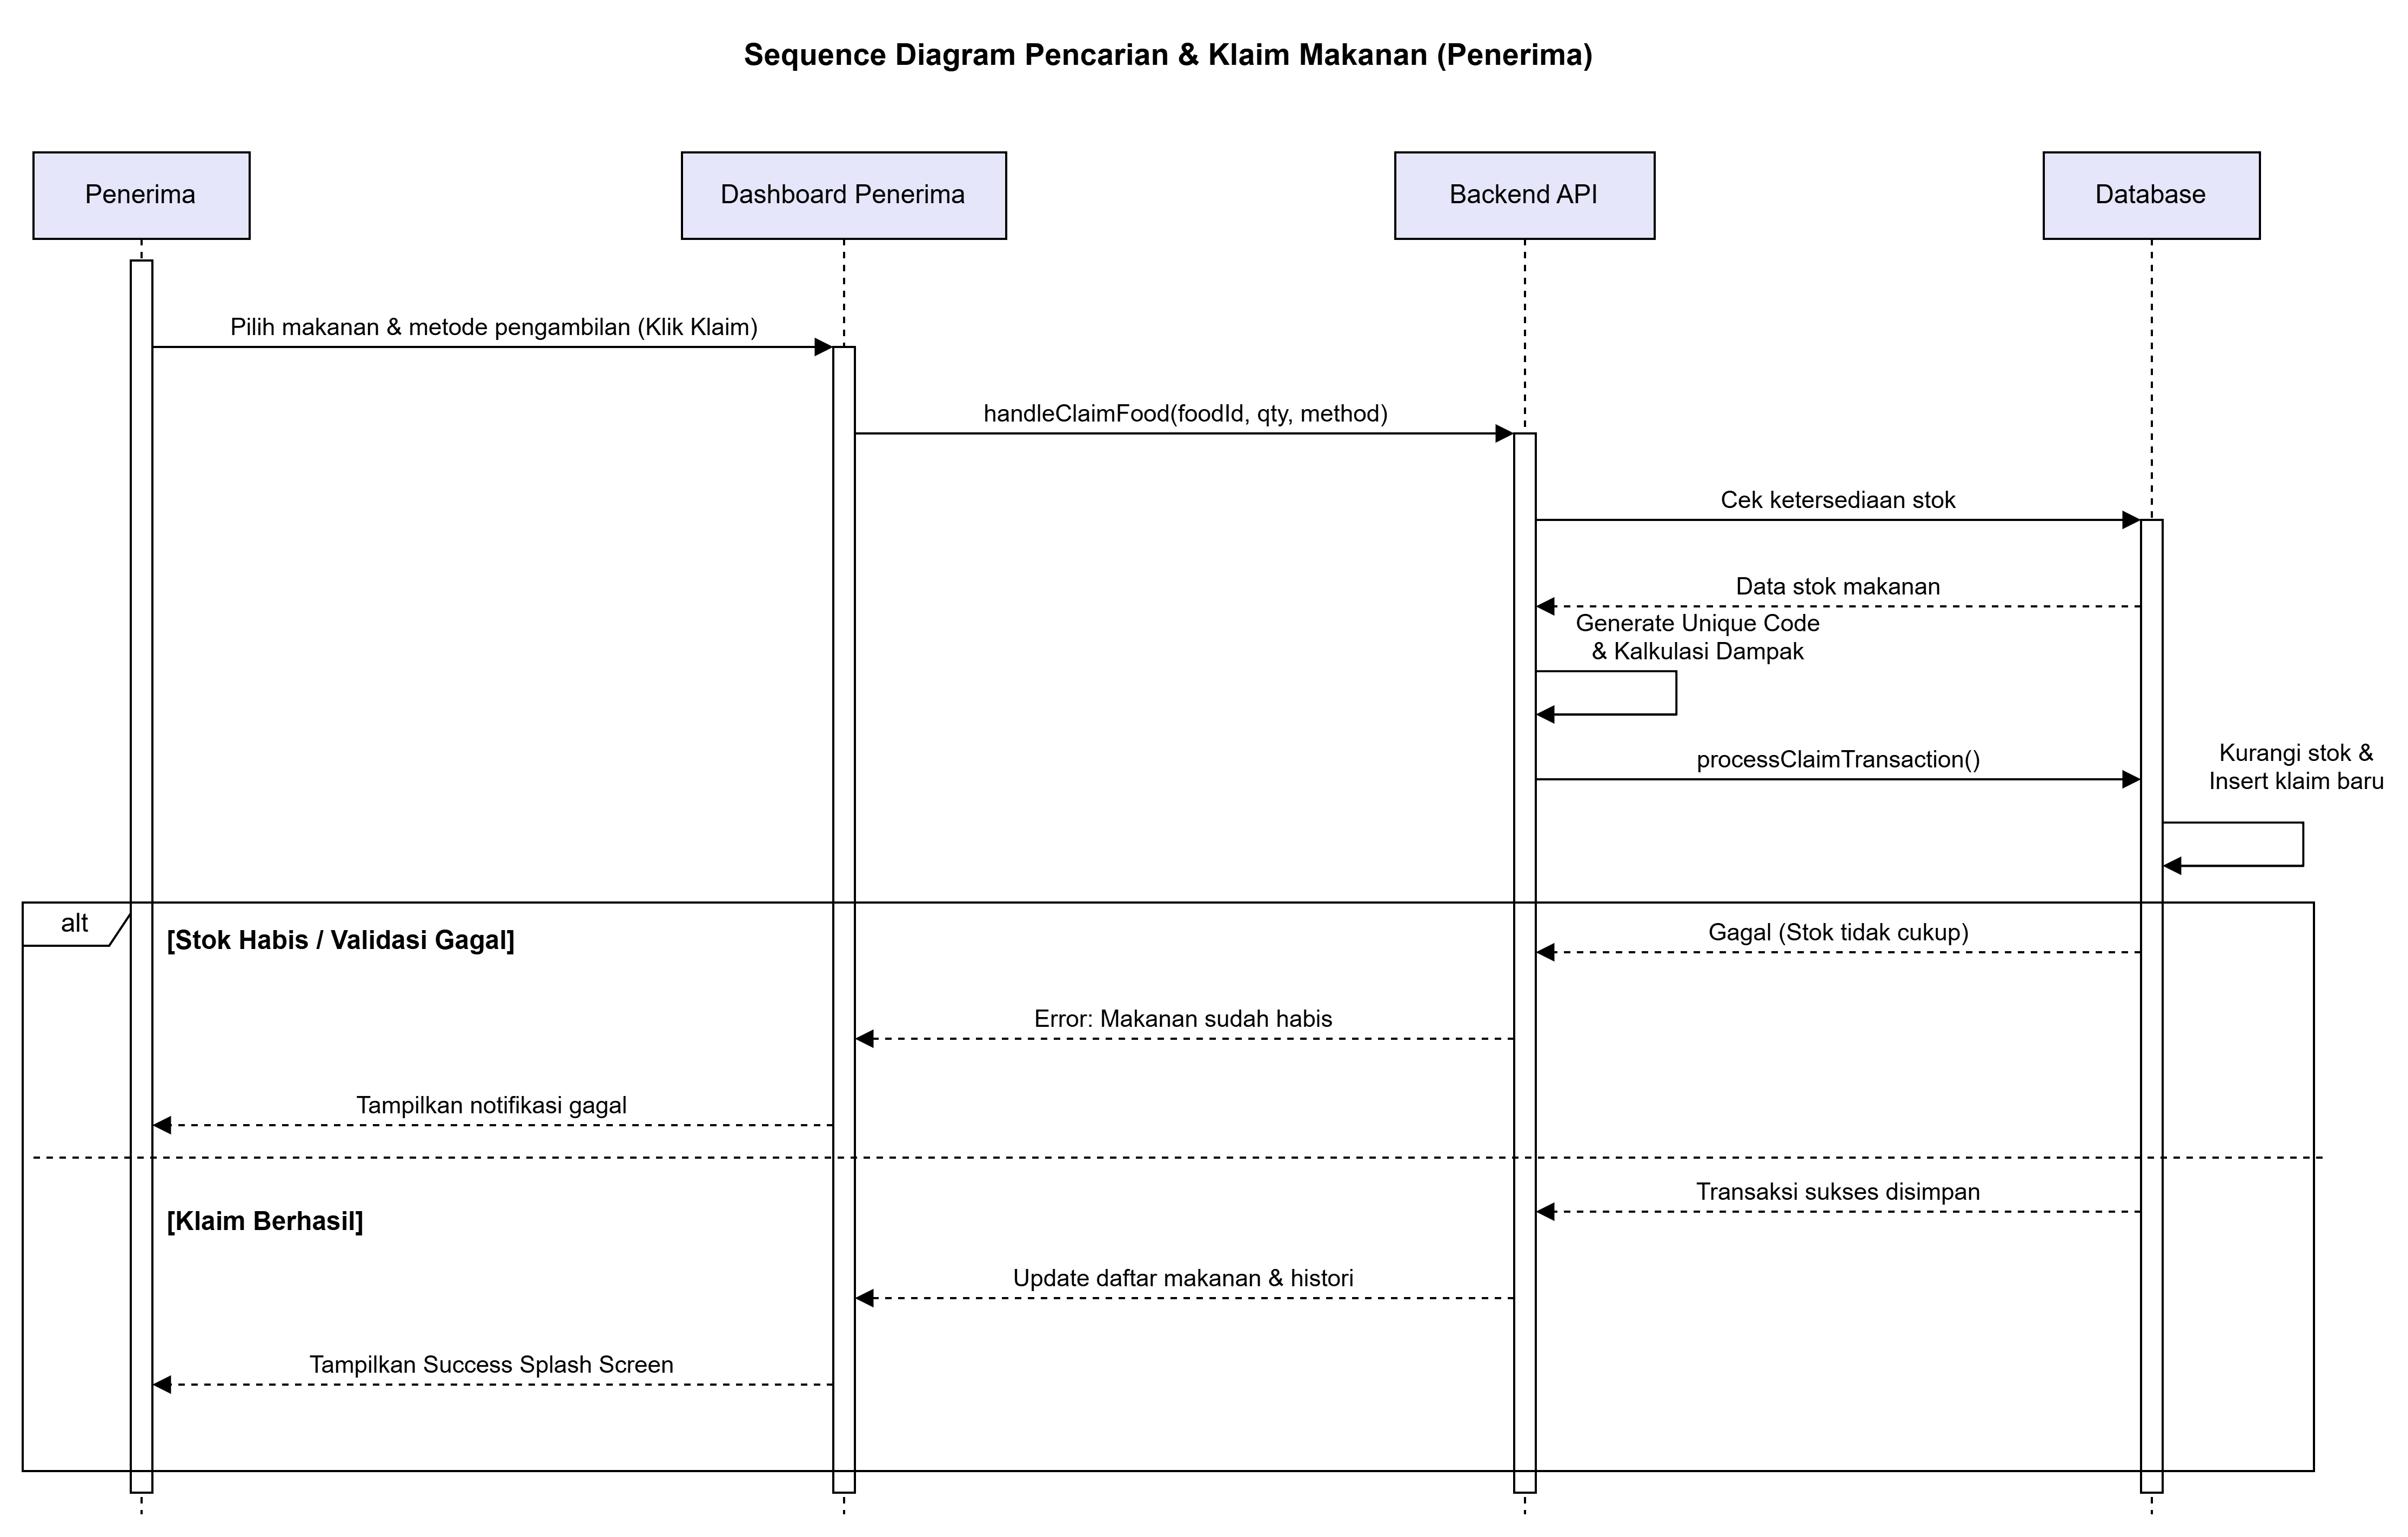
\includegraphics[width=1\textwidth]{image/bab3/sequence/Sequence Diagram Pencarian & Klaim Makanan (Penerima).png}
    \captionsetup{hypcap=false}
    \caption{\textit{Sequence Diagram} Pencarian \& Klaim Makanan (Penerima)}
    \label{fig:sd-klaim-penerima}
\end{figure}

\textbf{8. \textit{Sequence Diagram} Pelaporan Masalah}

Penerima mengisi alasan dan mengunggah bukti di \textit{Modal} Laporan (misal jika makanan rusak). \textit{Backend} memproses \texttt{handleSubmitReport}, menyimpan data ke \textit{Database} (memperbarui status klaim), dan memicu \texttt{insertAdminNotification()}. Jika sukses, lencana status klaim berubah menjadi ``Reported''.

\begin{figure}[H]
    \centering
    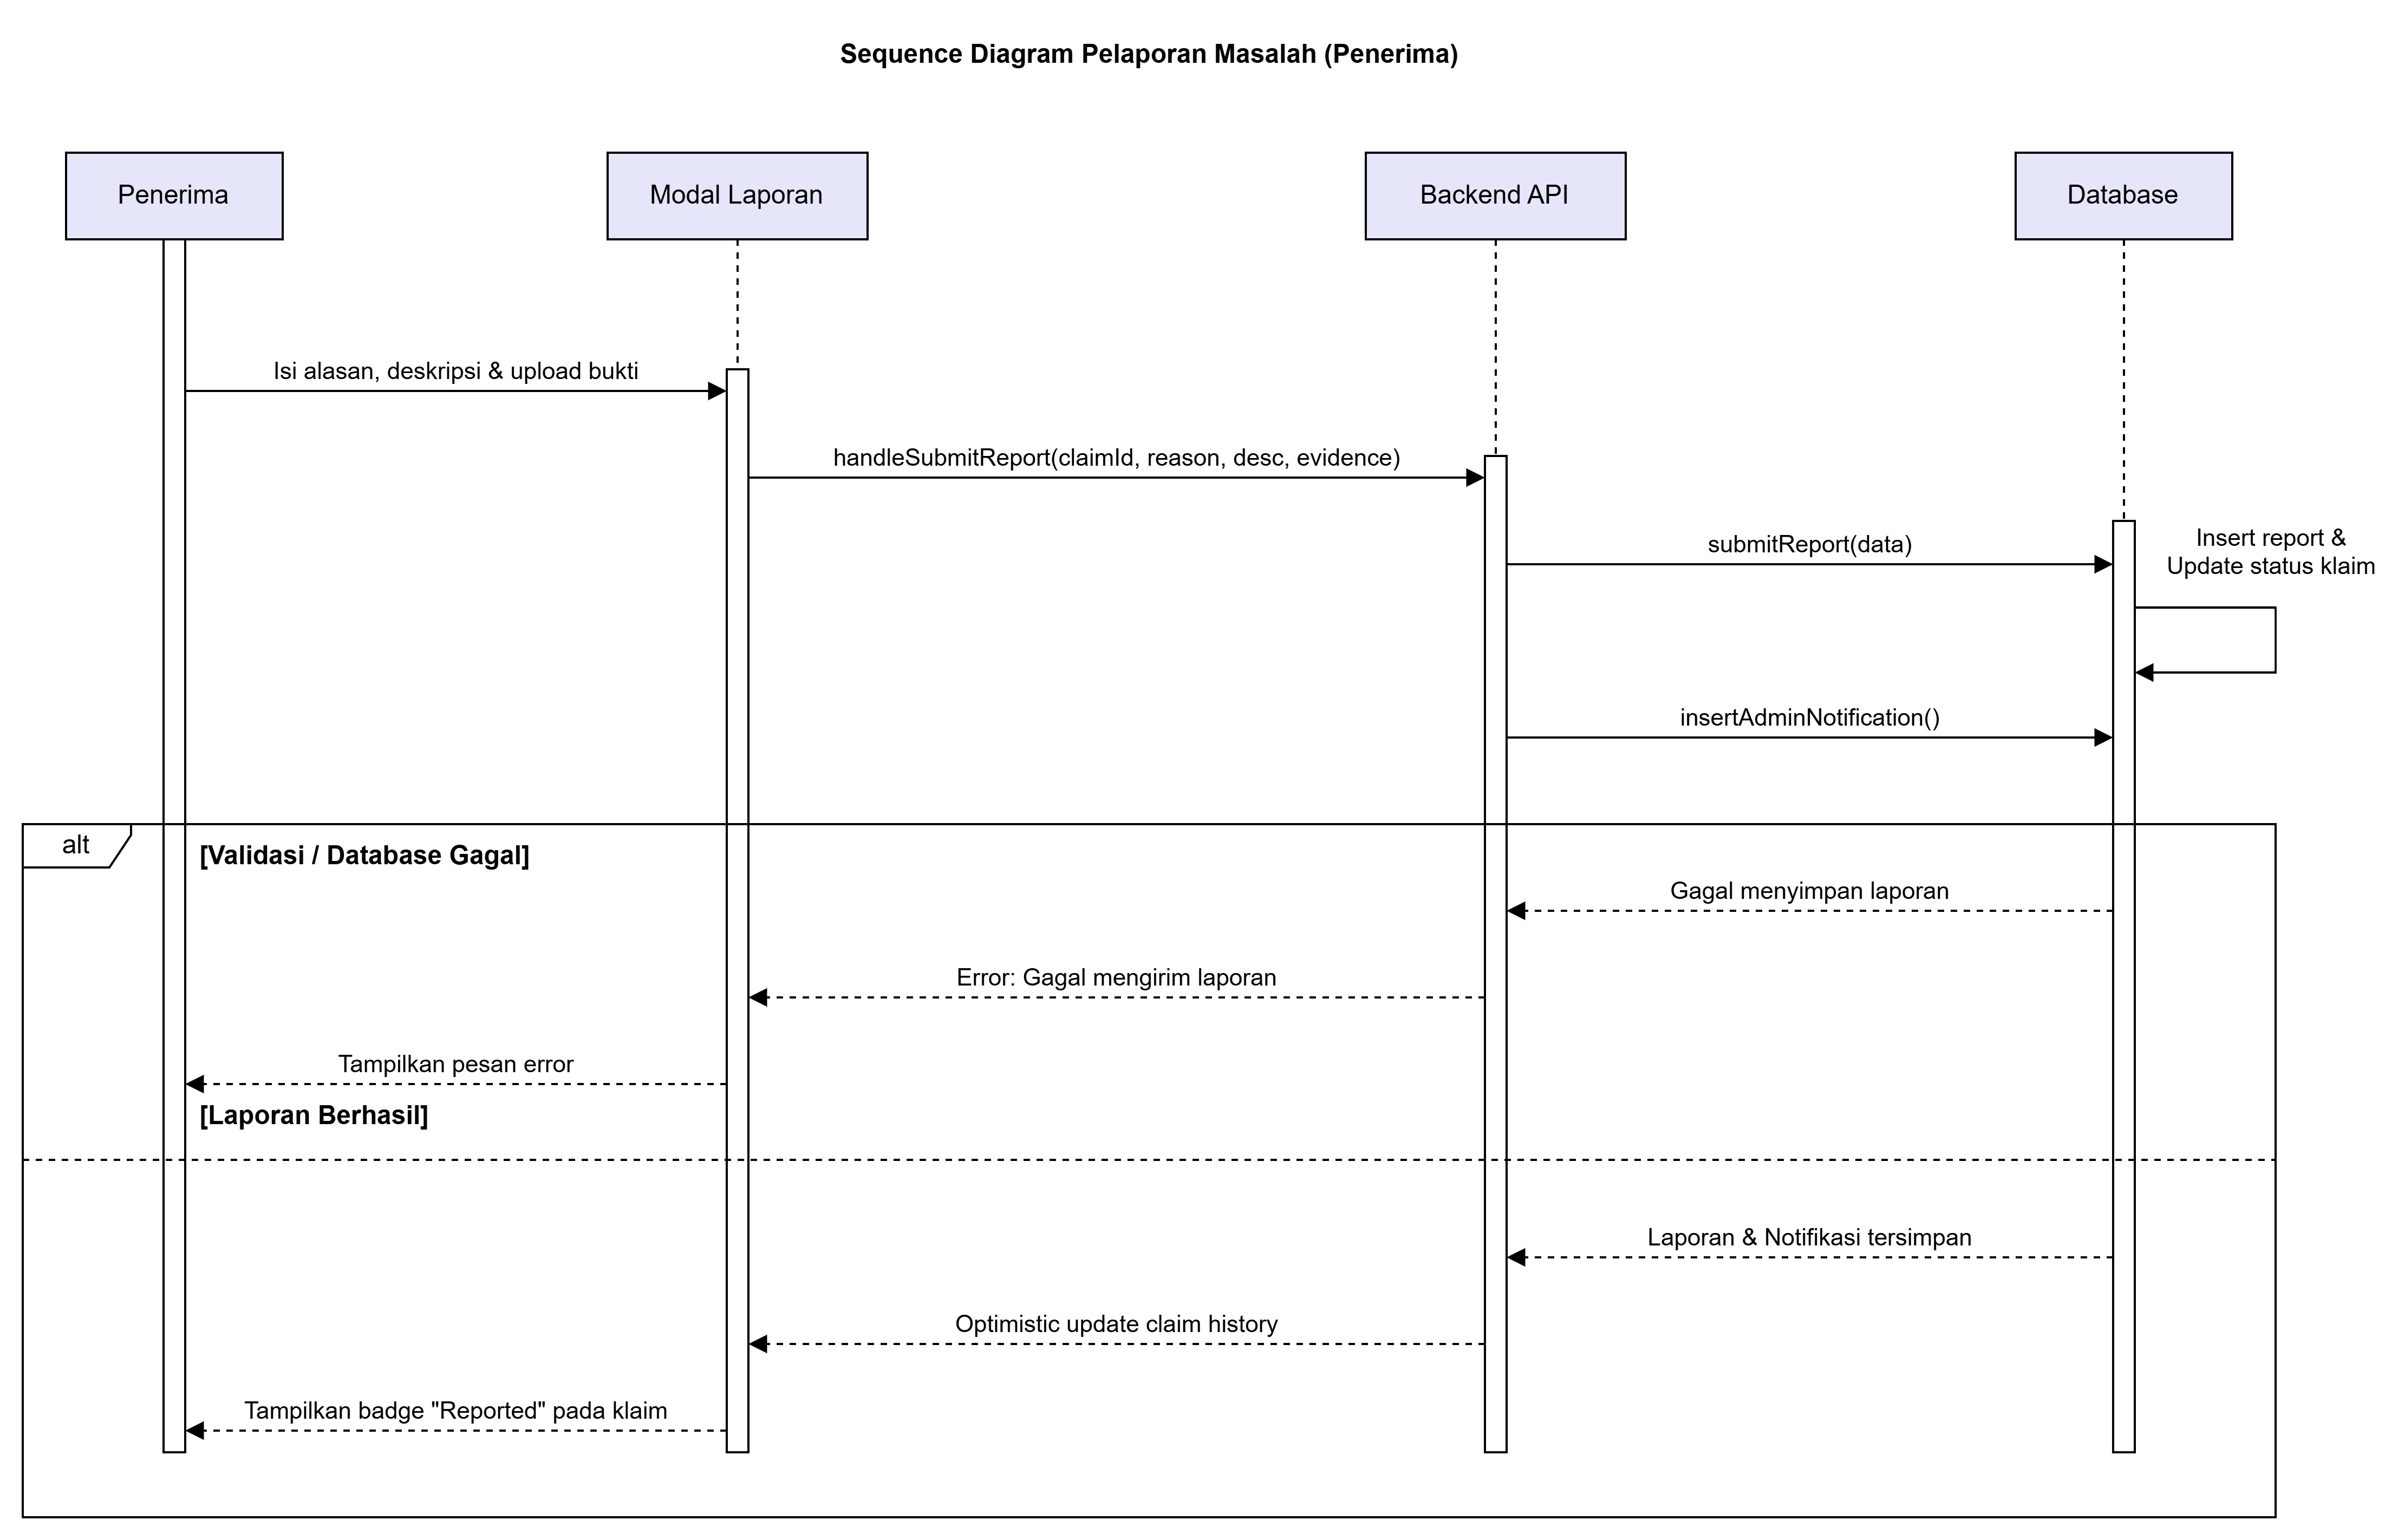
\includegraphics[width=1\textwidth]{image/bab3/sequence/Sequence Diagram Pelaporan Masalah (Penerima).png}
    \captionsetup{hypcap=false}
    \caption{\textit{Sequence Diagram} Pelaporan Masalah (Penerima)}
    \label{fig:sd-laporan-penerima}
\end{figure}

\textbf{9. \textit{Sequence Diagram} Pemberian Ulasan}

Setelah makanan diterima, Penerima mengisi \textit{rating} dan komentar. \textit{Backend} menerima \texttt{handleSubmitReview} dan menyimpannya ke \textit{Database}. Jika berhasil, kartu klaim pada riwayat pengguna akan diperbarui menjadi berstatus ``Reviewed''.

\begin{figure}[H]
    \centering
    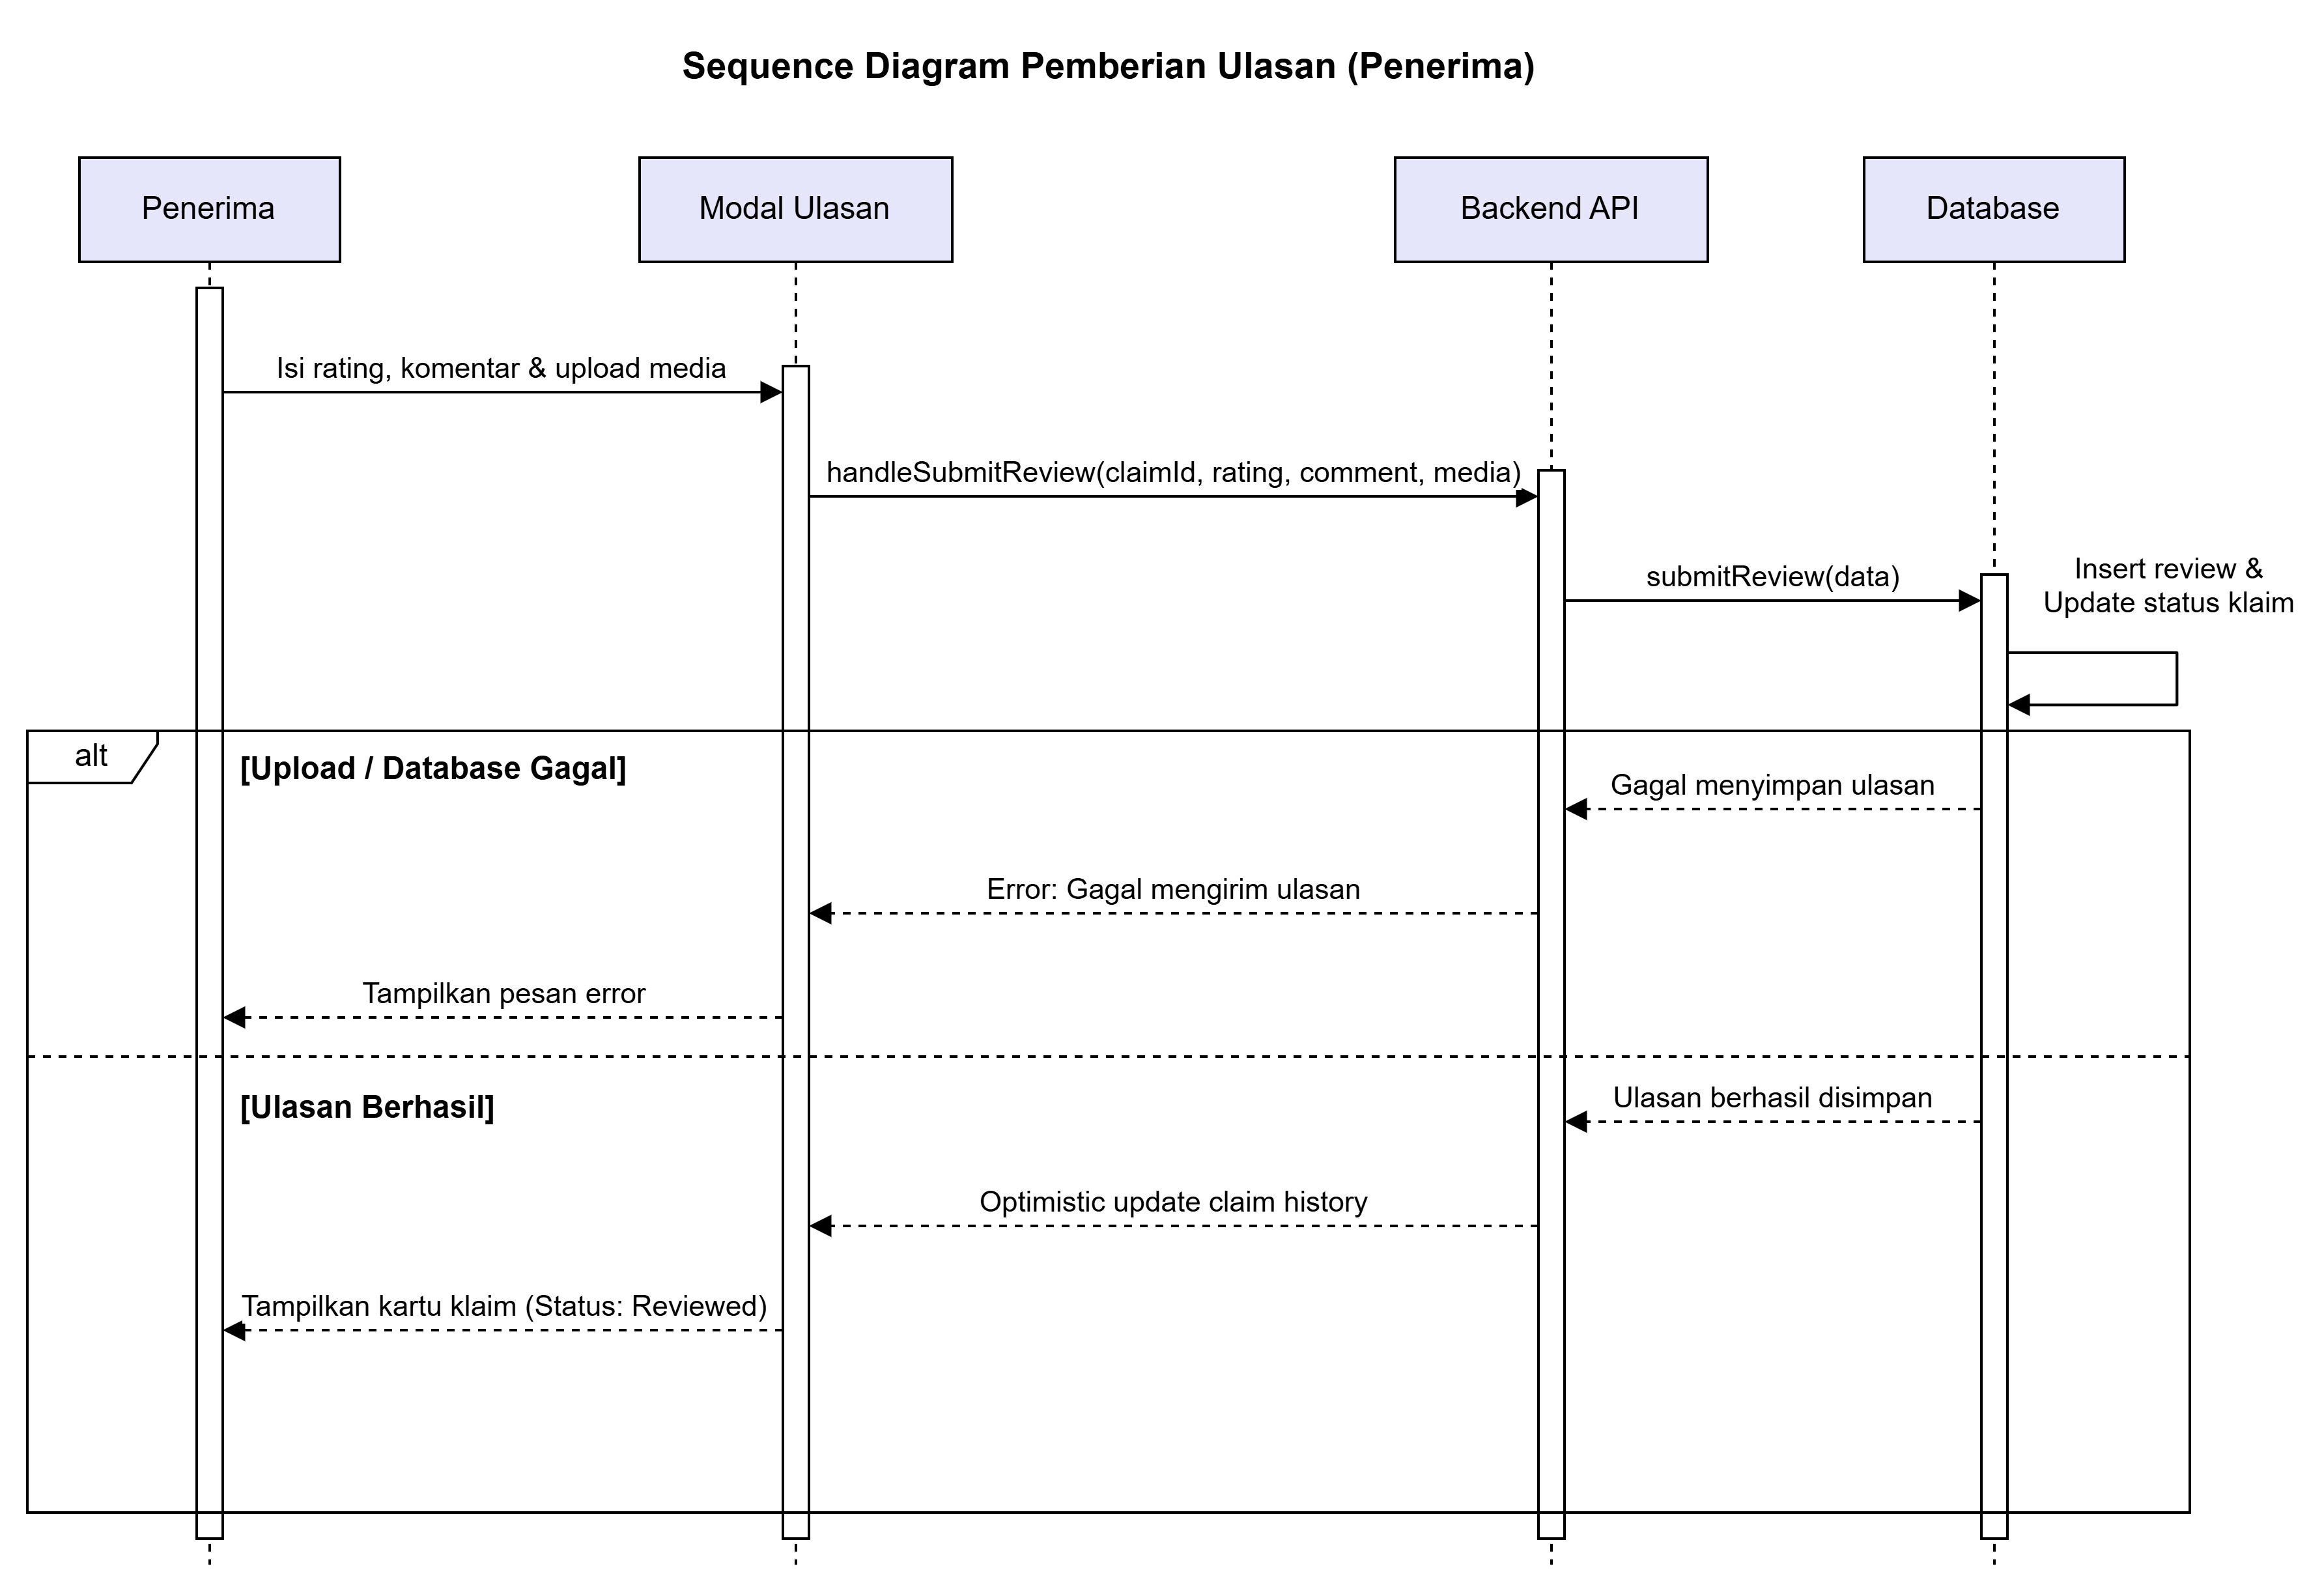
\includegraphics[width=1\textwidth]{image/bab3/sequence/Sequence Diagram Pemberian Ulasan (Penerima).png}
    \captionsetup{hypcap=false}
    \caption{\textit{Sequence Diagram} Pemberian Ulasan (Penerima)}
    \label{fig:sd-ulasan-penerima}
\end{figure}

% ------------------------------------------------------------------
\subsubsection{Alur Relawan}
% ------------------------------------------------------------------

\textbf{10. \textit{Sequence Diagram} Penerimaan Misi Pengantaran}

Relawan memilih misi dari \textit{Missions Board} dan mengklik ``Ambil Misi''. \textit{Backend} mengecek status transaksi di \textit{Database}. Jika status masih \textit{PENDING}, \textit{Backend} menetapkan ID Relawan (\texttt{volunteer\_id}) dan mengubah status menjadi \textit{IN\_PROGRESS}. Rute navigasi kemudian ditampilkan. Jika misi sudah diambil orang lain, sistem akan menolak dan memperbarui daftar misi.

\begin{figure}[H]
    \centering
    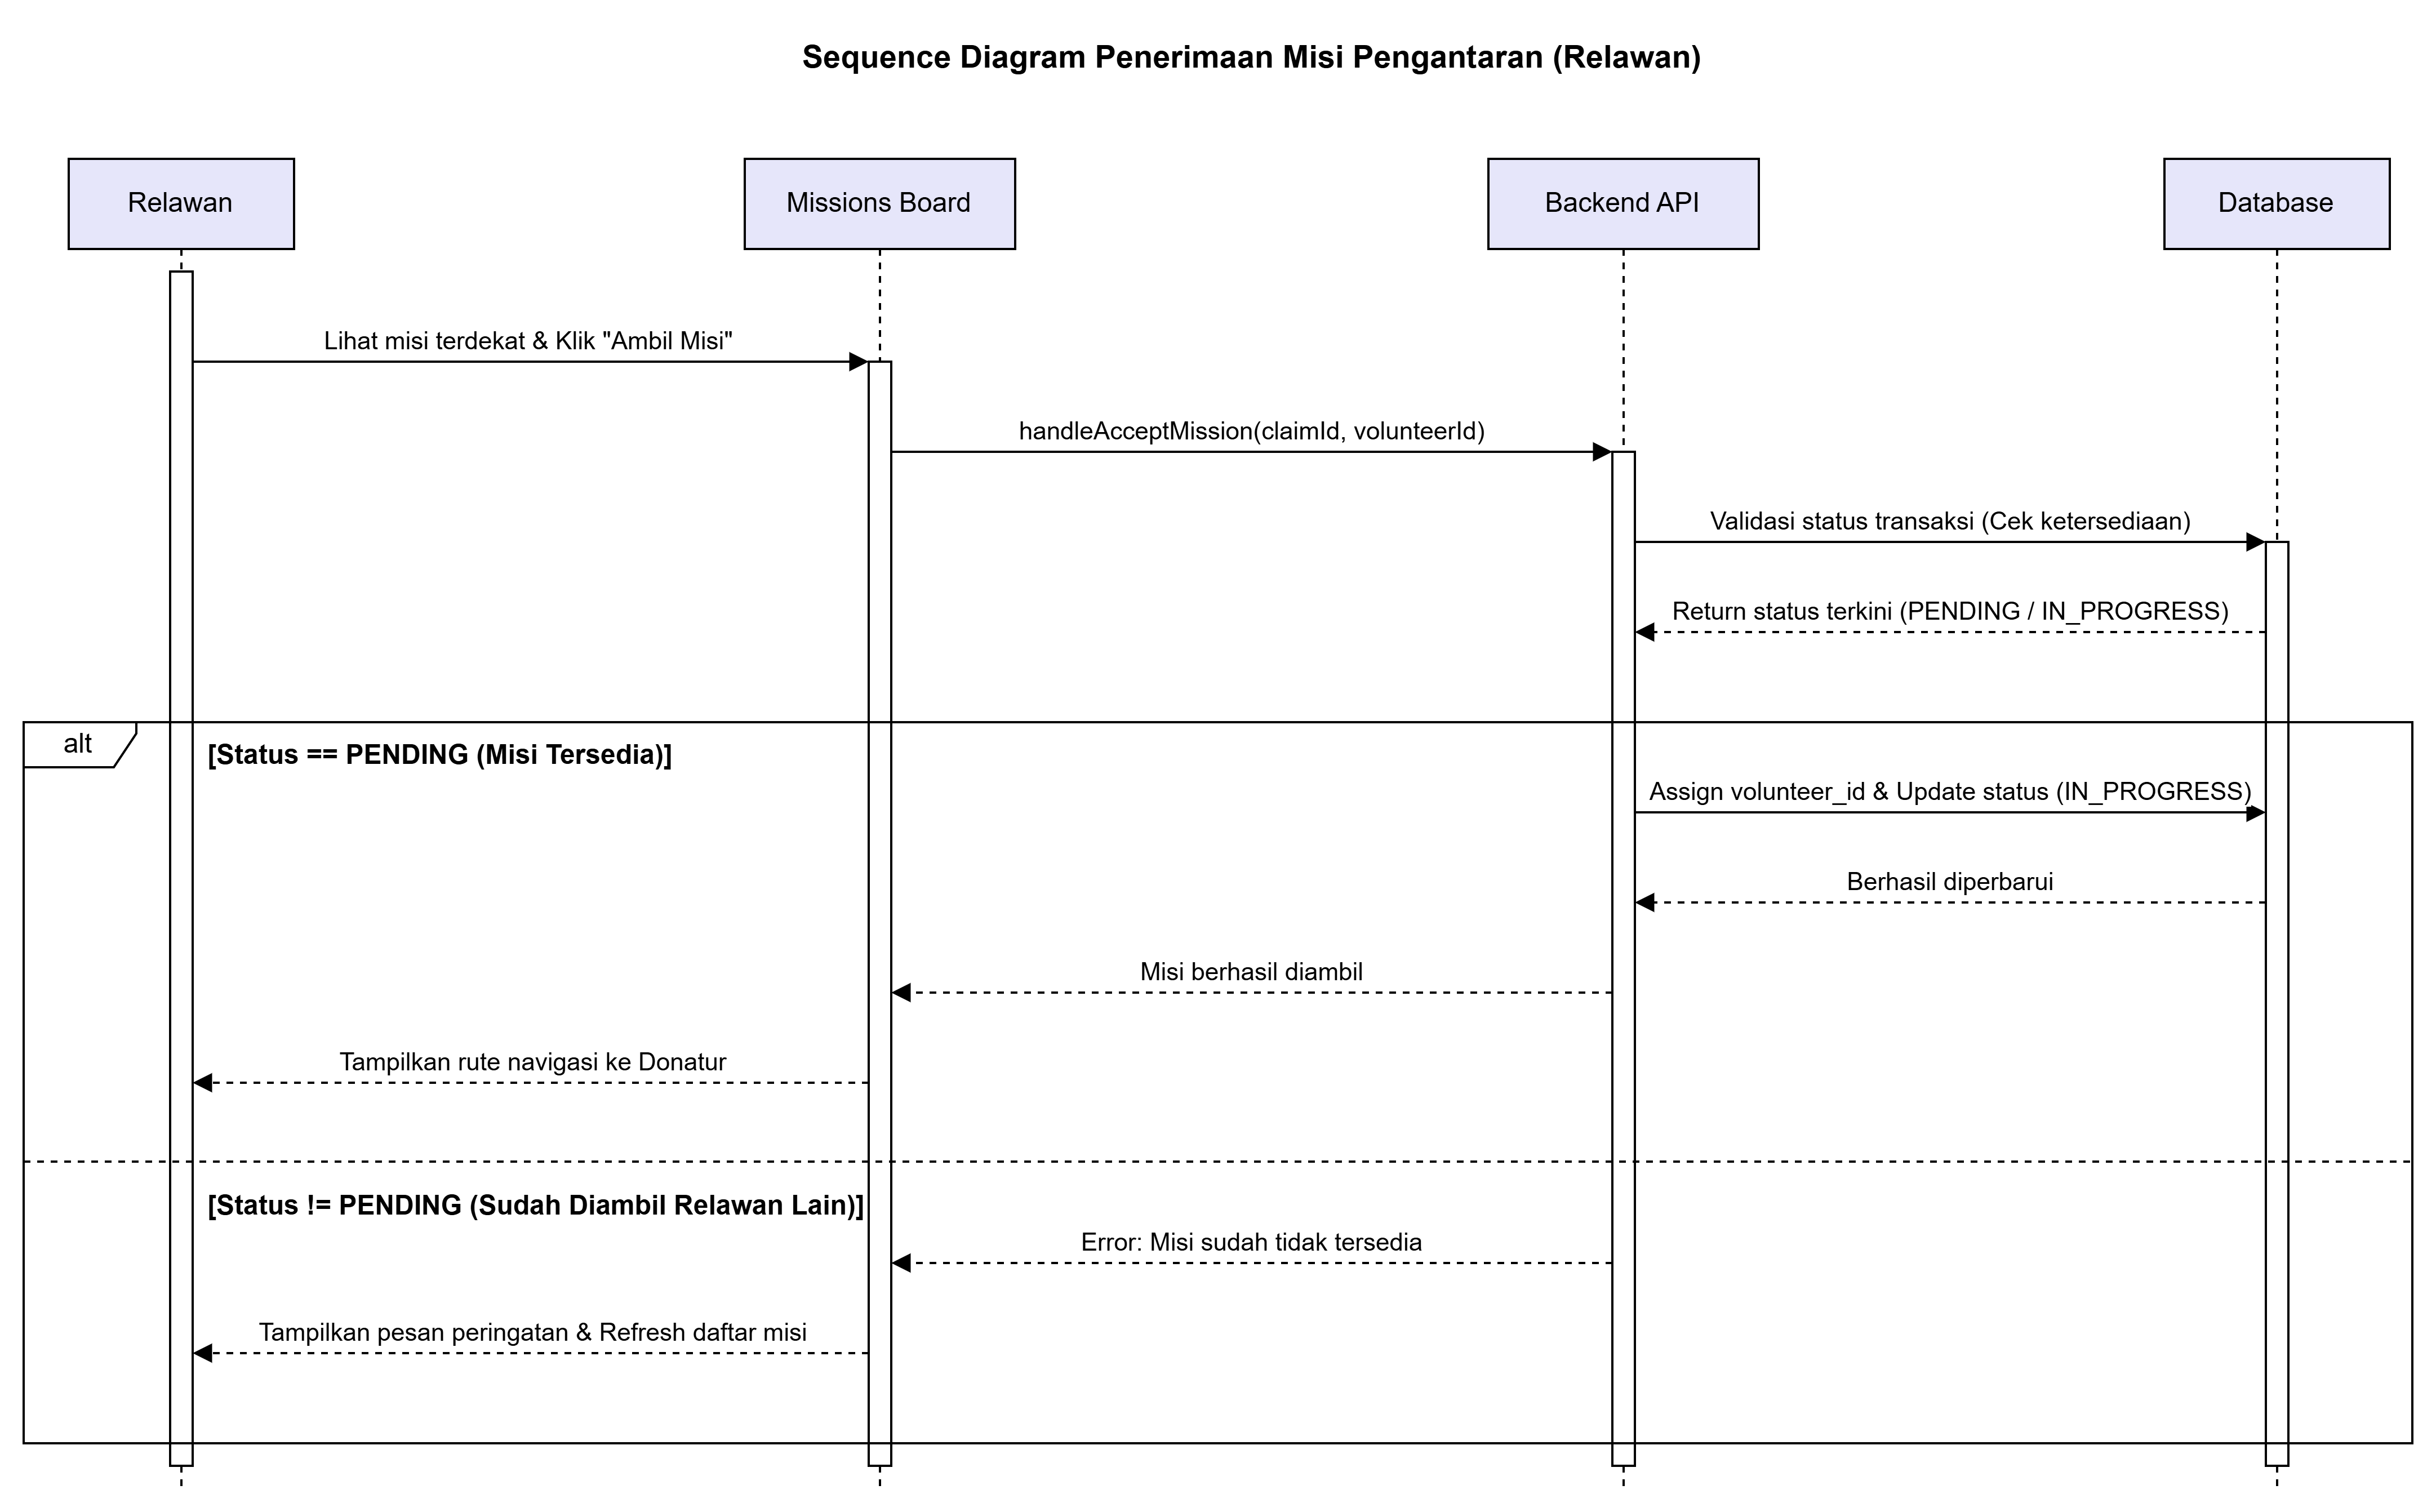
\includegraphics[width=1\textwidth]{image/bab3/sequence/Sequence Diagram Penerimaan Misi Pengantaran (Relawan).png}
    \captionsetup{hypcap=false}
    \caption{\textit{Sequence Diagram} Penerimaan Misi Pengantaran (Relawan)}
    \label{fig:sd-misi-relawan}
\end{figure}

\textbf{11. \textit{Sequence Diagram} Validasi Serah Terima (QR Code / Manual)}

Saat mengantar makanan, Relawan memindai QR Code Penerima menggunakan kamera atau mengetik \textit{Unique Code} 6-digit secara manual. \textit{Backend} memverifikasi \texttt{handleVerifyCode} dengan data di \textit{Database}. Jika cocok, status klaim diubah menjadi \textit{COMPLETED}, dan \textit{Backend} langsung memicu (\textit{trigger}) \texttt{GamificationService}.

\begin{figure}[H]
    \centering
    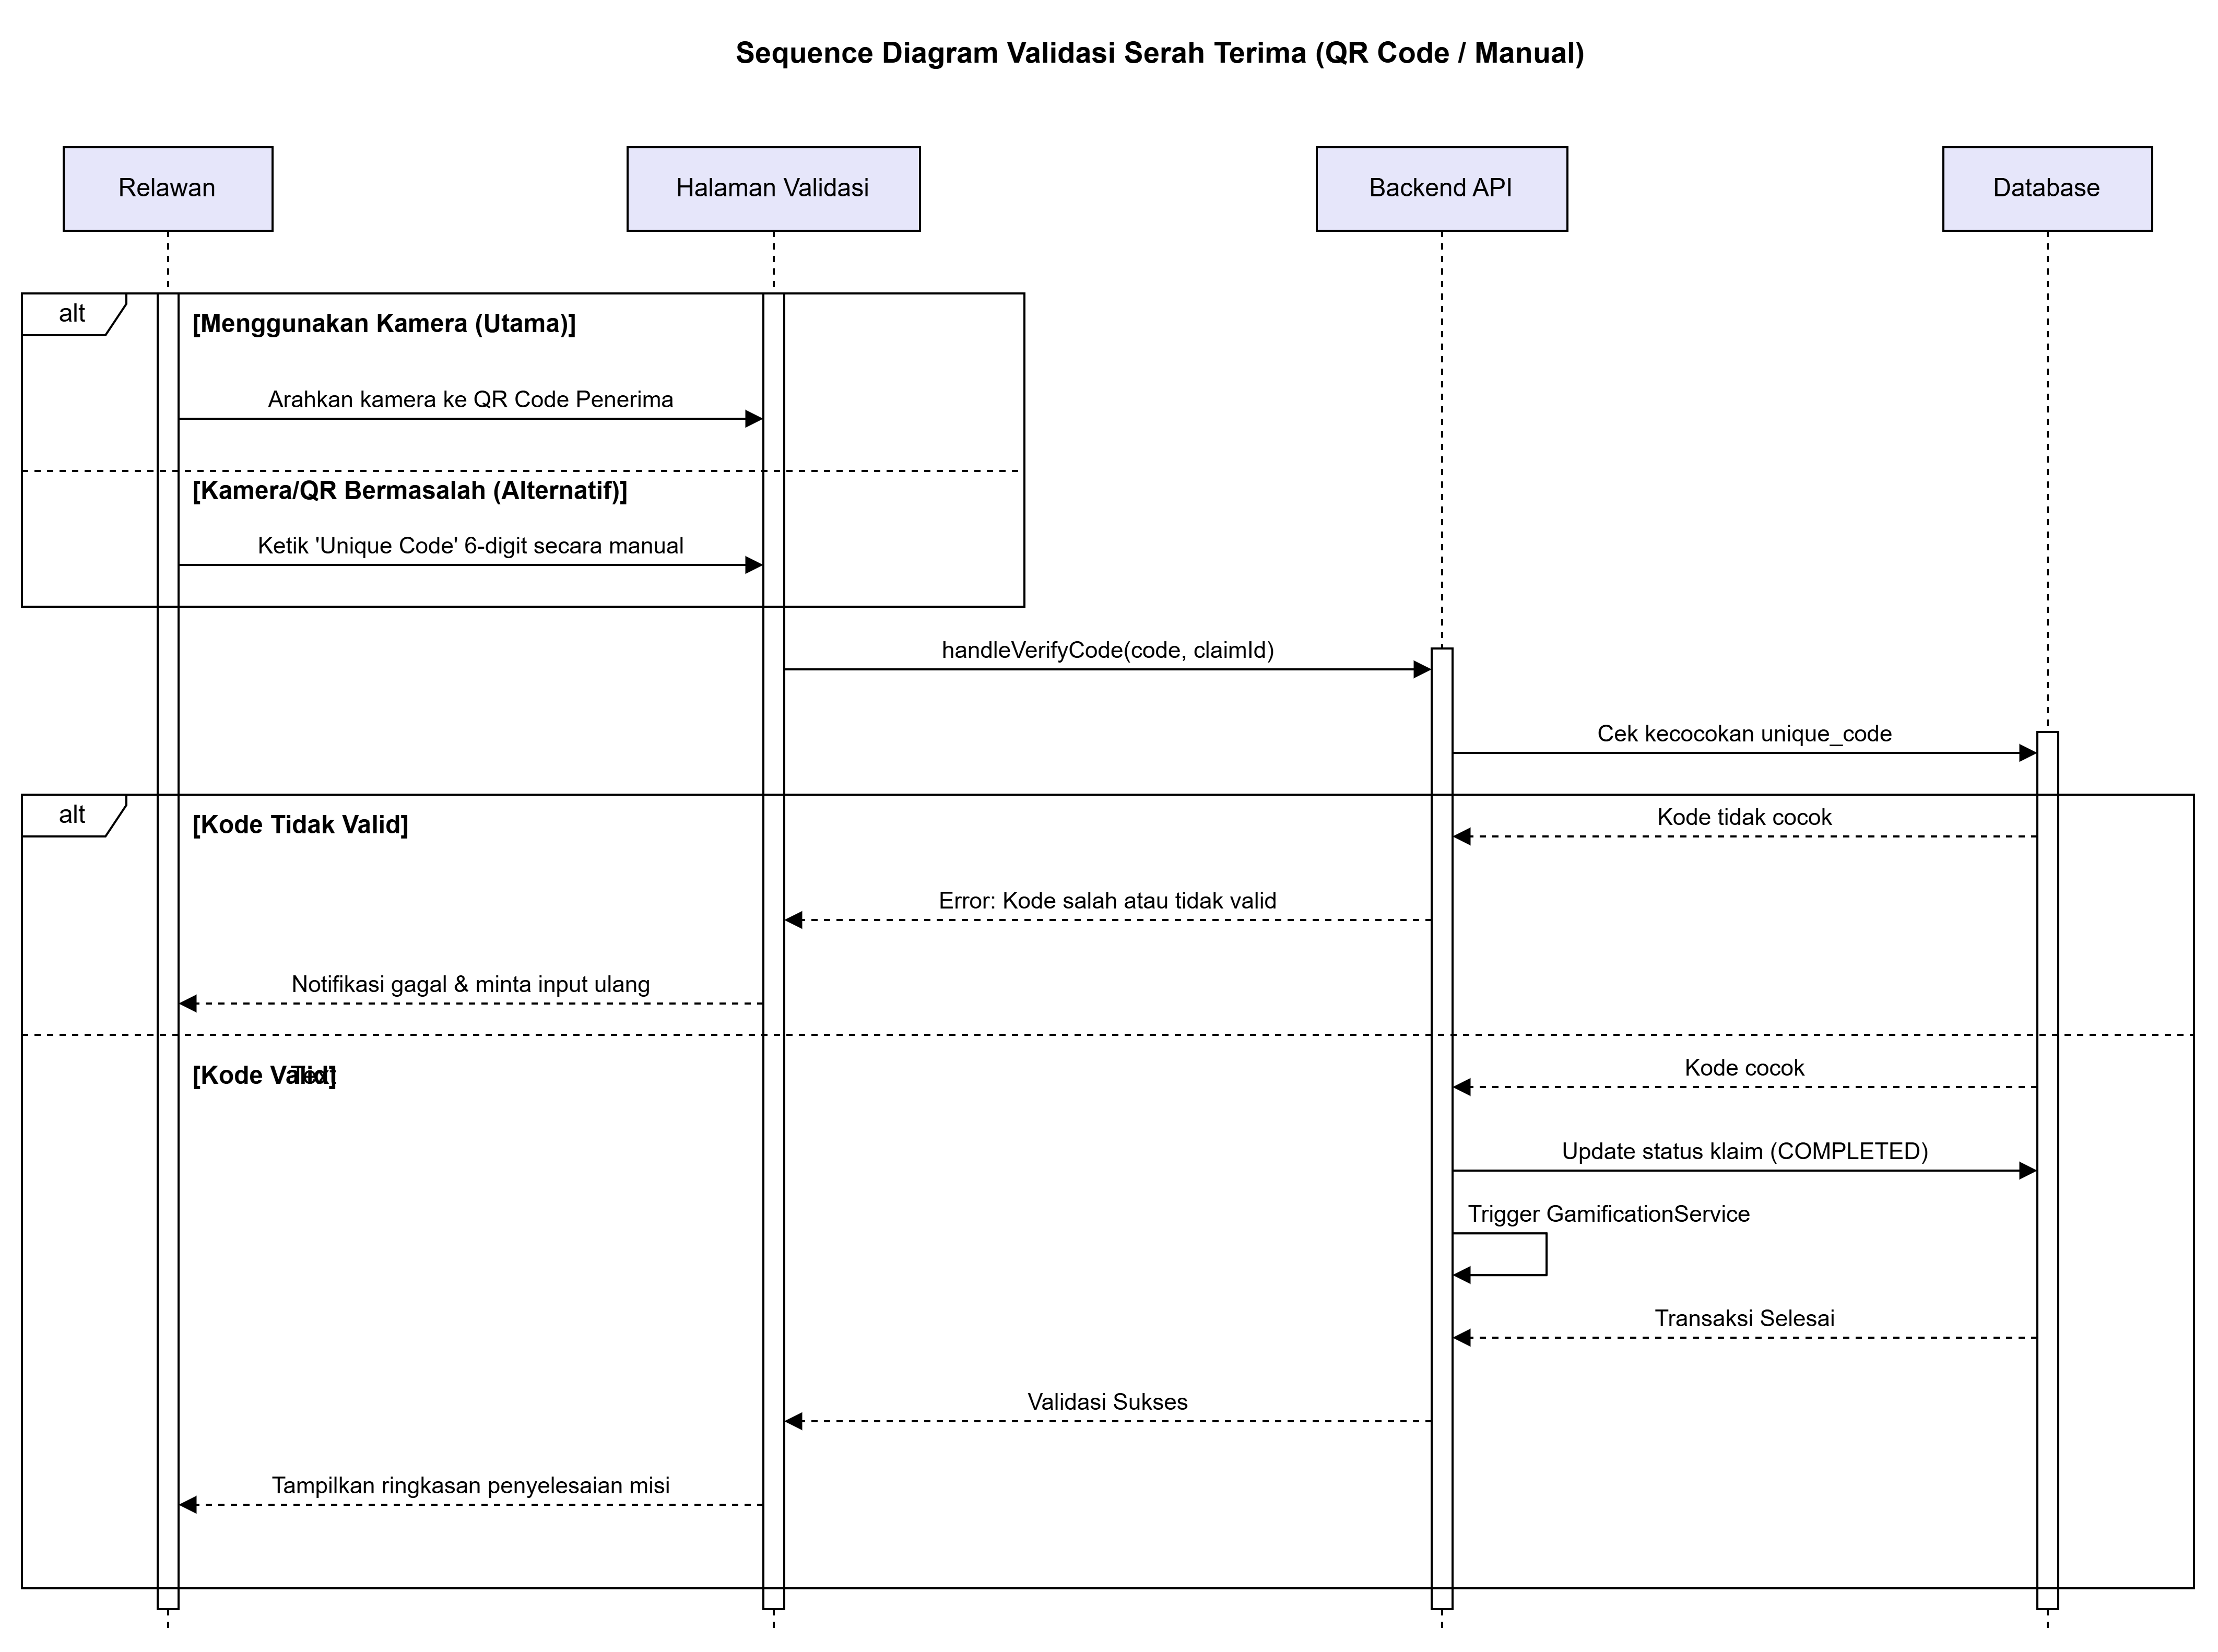
\includegraphics[width=1\textwidth]{image/bab3/sequence/Sequence Diagram Validasi Serah Terima (Relawan).png}
    \captionsetup{hypcap=false}
    \caption{\textit{Sequence Diagram} Validasi Serah Terima (Relawan)}
    \label{fig:sd-serahterima-relawan}
\end{figure}

% ------------------------------------------------------------------
\subsubsection{Alur Sistem Internal}
% ------------------------------------------------------------------

\textbf{12. \textit{Sequence Diagram} Kalkulasi Gamifikasi XP \& \textit{Badge}}

Berjalan di latar belakang tanpa interaksi langsung pengguna. Setelah validasi serah terima berhasil, \textit{Backend} meminta \texttt{calculateXP} ke \textit{Gamification Service}. Layanan mengambil poin dampak dari \textit{Database}, lalu menambahkannya ke ID Relawan. Selanjutnya, \texttt{evaluateRank} mengevaluasi total poin. Jika memenuhi syarat naik pangkat, lencana (\textit{badge}) dan \textit{rank} pengguna akan otomatis diperbarui di \textit{database}.

\begin{figure}[H]
    \centering
    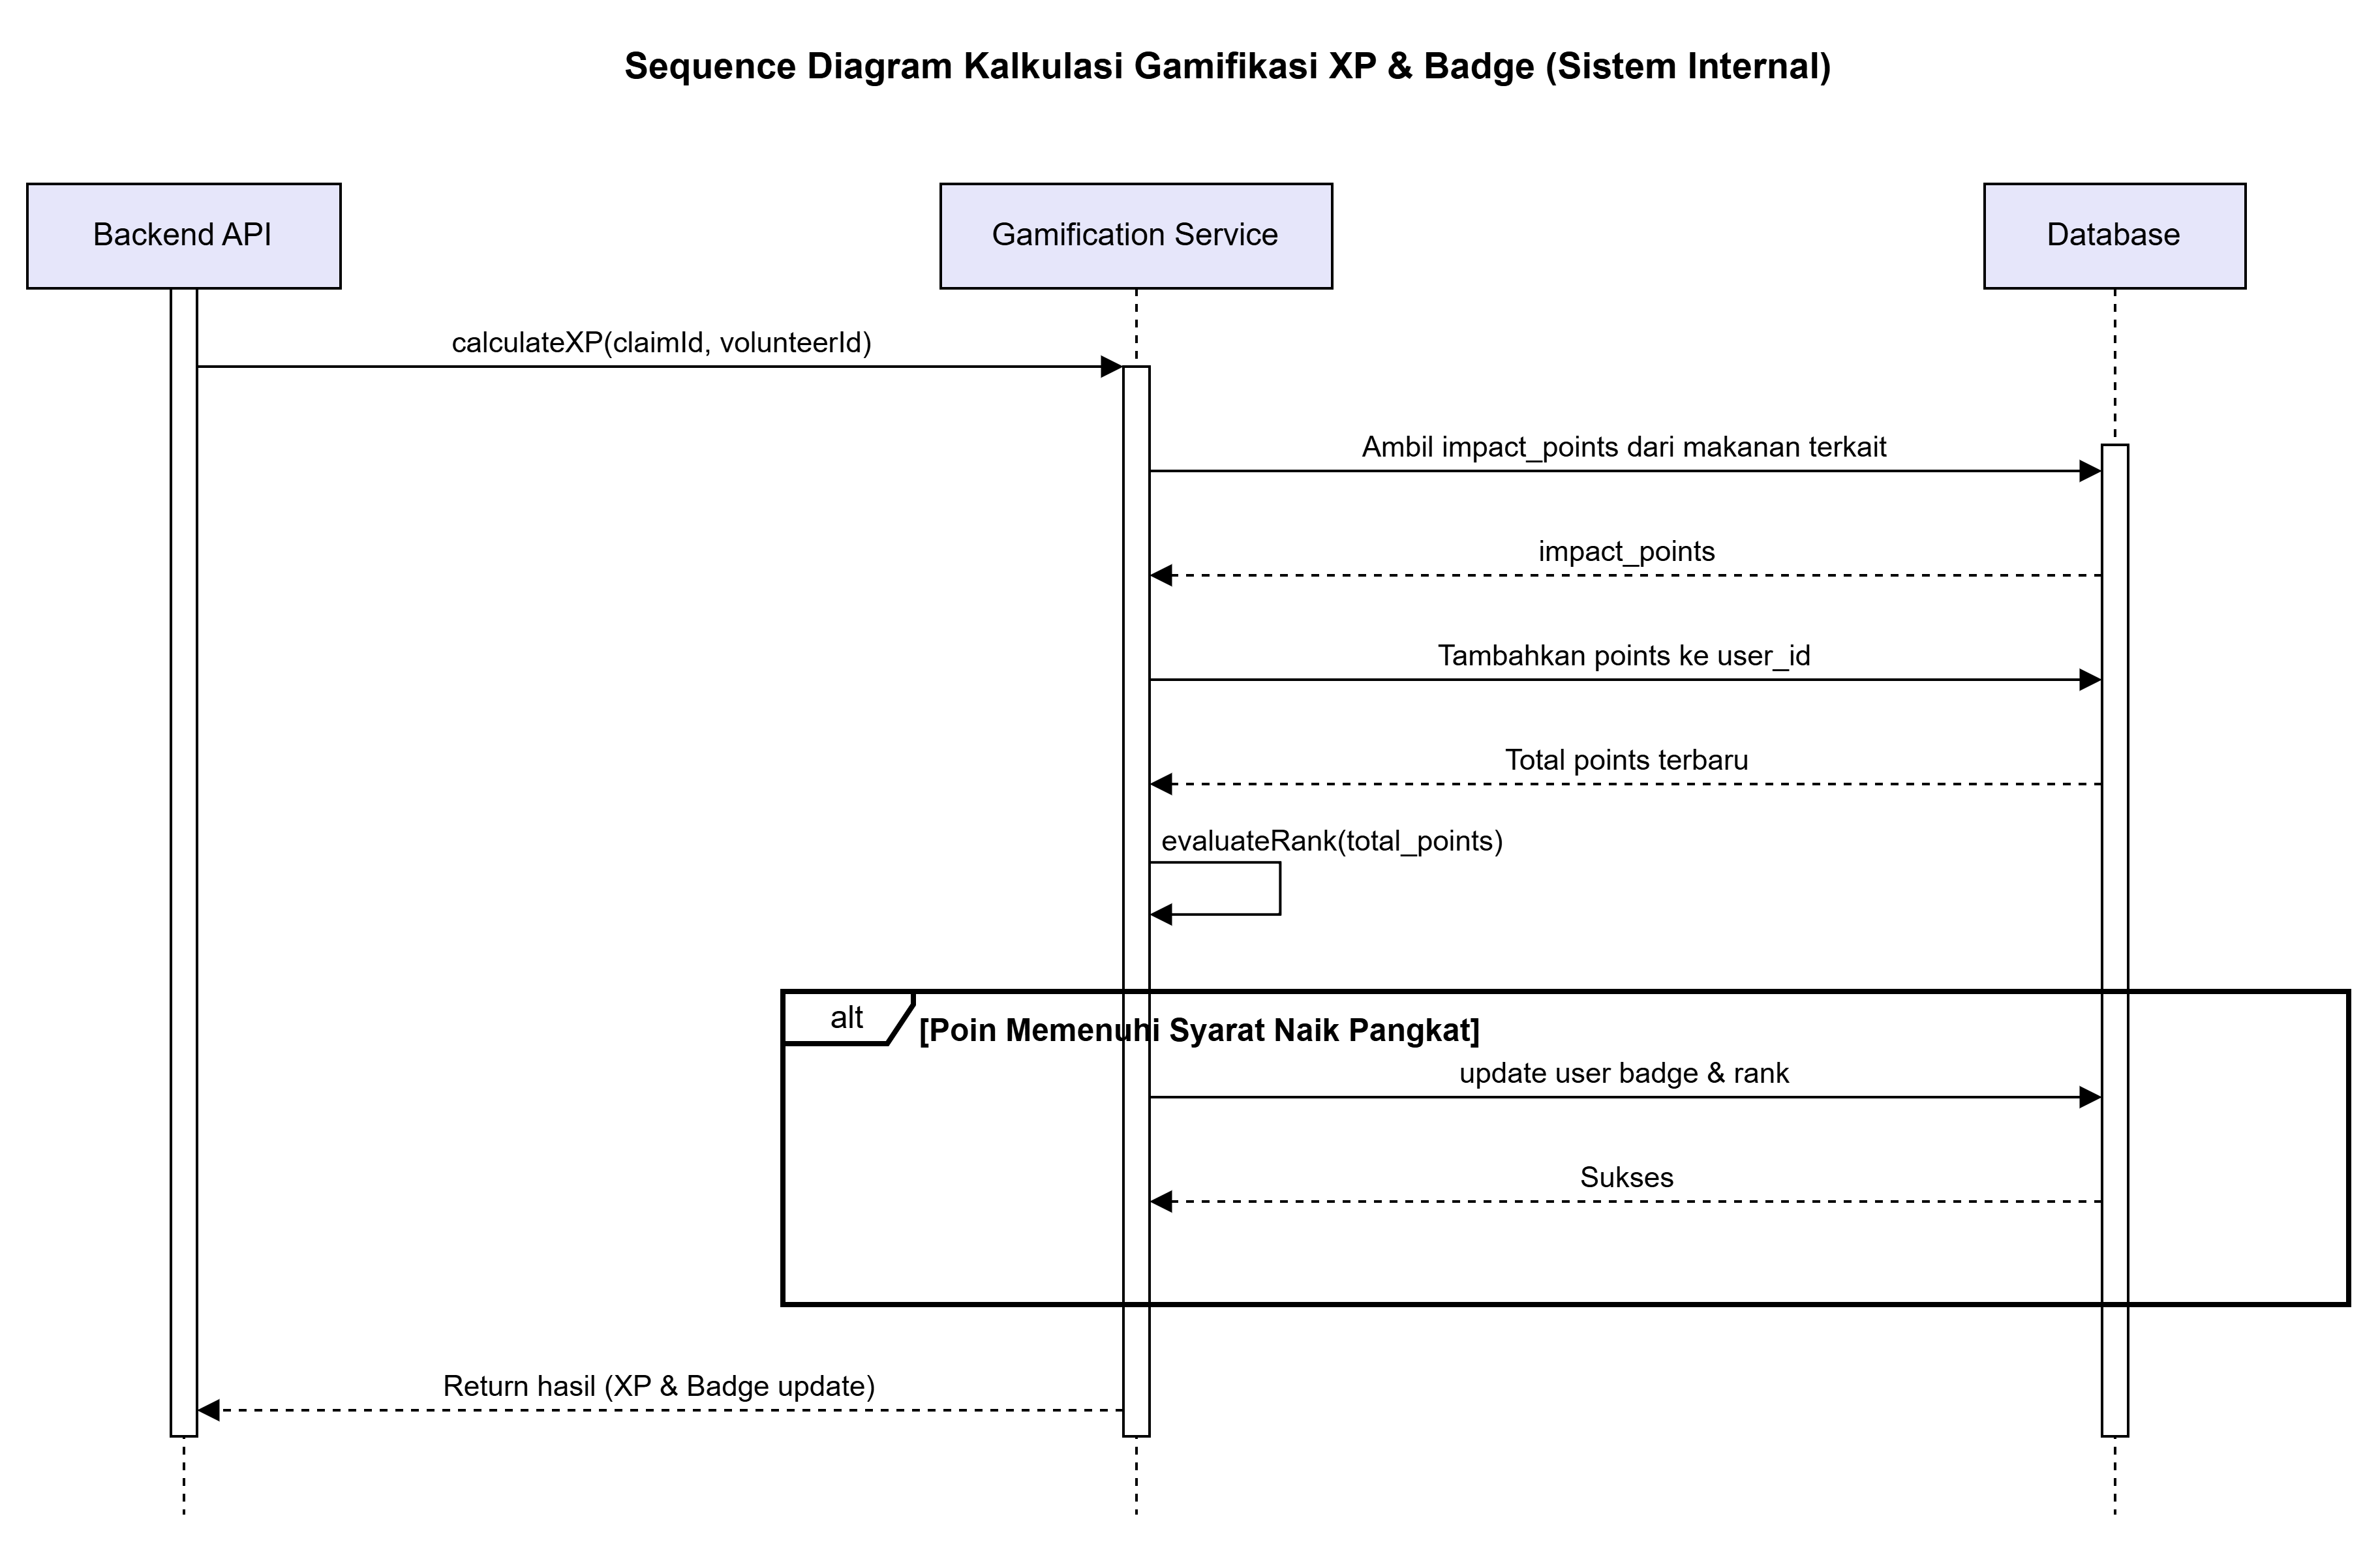
\includegraphics[width=1\textwidth]{image/bab3/sequence/Sequence Diagram Kalkulasi Gamifikasi (Sistem Internal).png}
    \captionsetup{hypcap=false}
    \caption{\textit{Sequence Diagram} Kalkulasi Gamifikasi (Sistem Internal)}
    \label{fig:sd-gamifikasi}
\end{figure}

% ------------------------------------------------------------------
\subsubsection{Alur Admin \& Super Admin}
% ------------------------------------------------------------------

\textbf{13. \textit{Sequence Diagram} Verifikasi Akun (Admin)}

Admin memilih akun pendaftar baru dan mengklik ``Verifikasi'' di \textit{User Manager}. \textit{Backend} memproses \texttt{handleVerifyUser} dan memperbarui status pengguna menjadi \textit{ACTIVE} atau \textit{REJECTED} di \textit{Database}. Setelah itu, sistem mengirimkan email notifikasi ke pendaftar, dan antarmuka Admin menampilkan status hijau.

\begin{figure}[H]
    \centering
    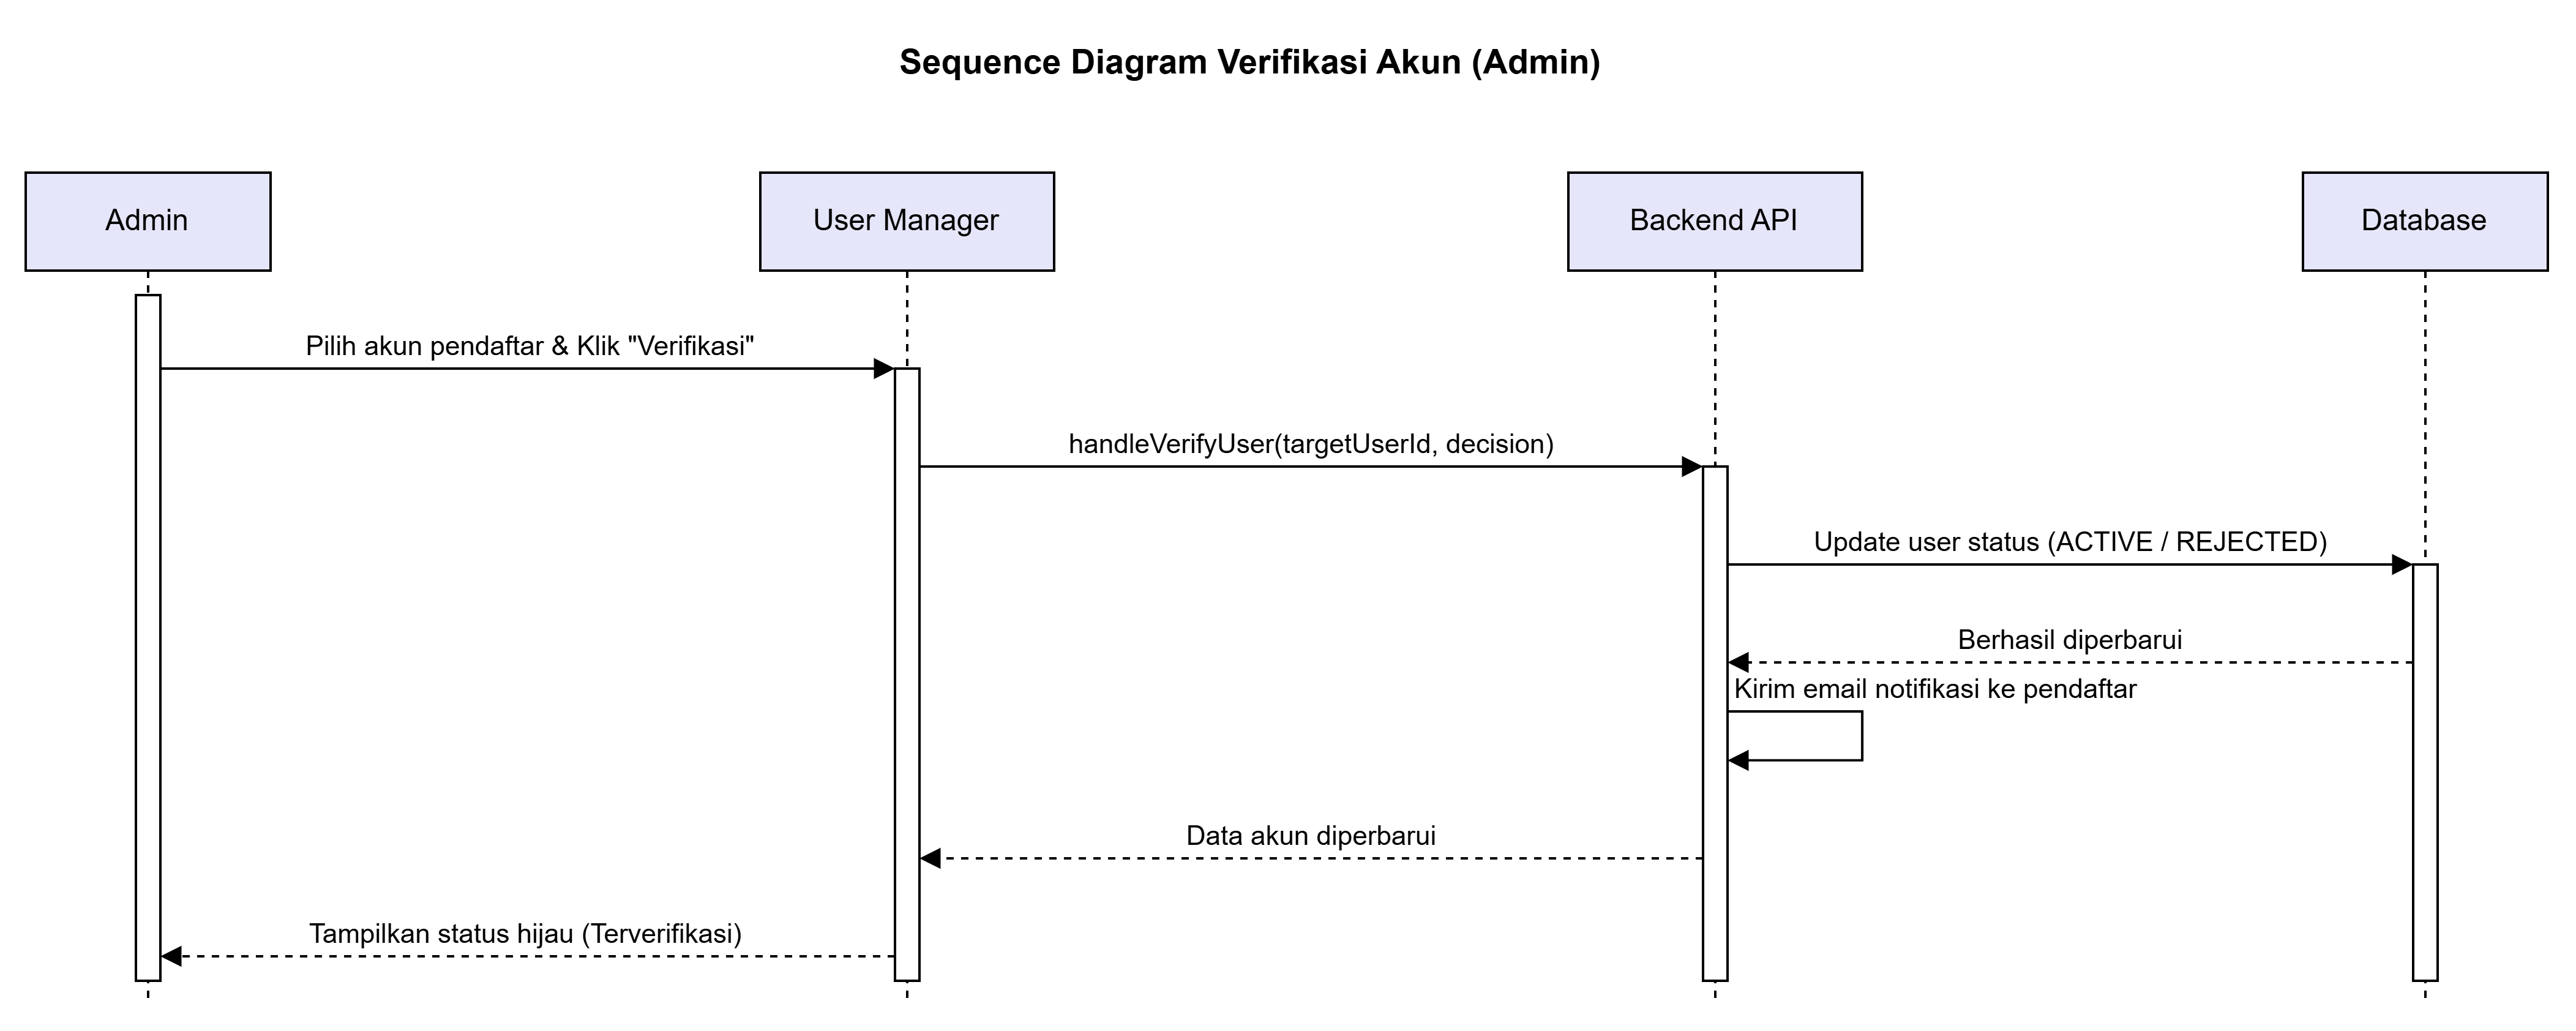
\includegraphics[width=1\textwidth]{image/bab3/sequence/Sequence Diagram Verifikasi Akun (Admin).png}
    \captionsetup{hypcap=false}
    \caption{\textit{Sequence Diagram} Verifikasi Akun (Admin Pengelola)}
    \label{fig:sd-verifikasi-admin}
\end{figure}

\textbf{14. \textit{Sequence Diagram} Moderasi Komplain (Admin)}

Admin meninjau laporan keluhan pengguna di halaman \textit{Support Request} dan memberikan keputusan. \textit{Backend} menjalankan \texttt{handleResolveReport}, lalu memperbarui tabel laporan menjadi \textit{RESOLVED} dan menyesuaikan status klaim di \textit{Database}. Kasus kemudian dihapus dari antrean aktif.

\begin{figure}[H]
    \centering
    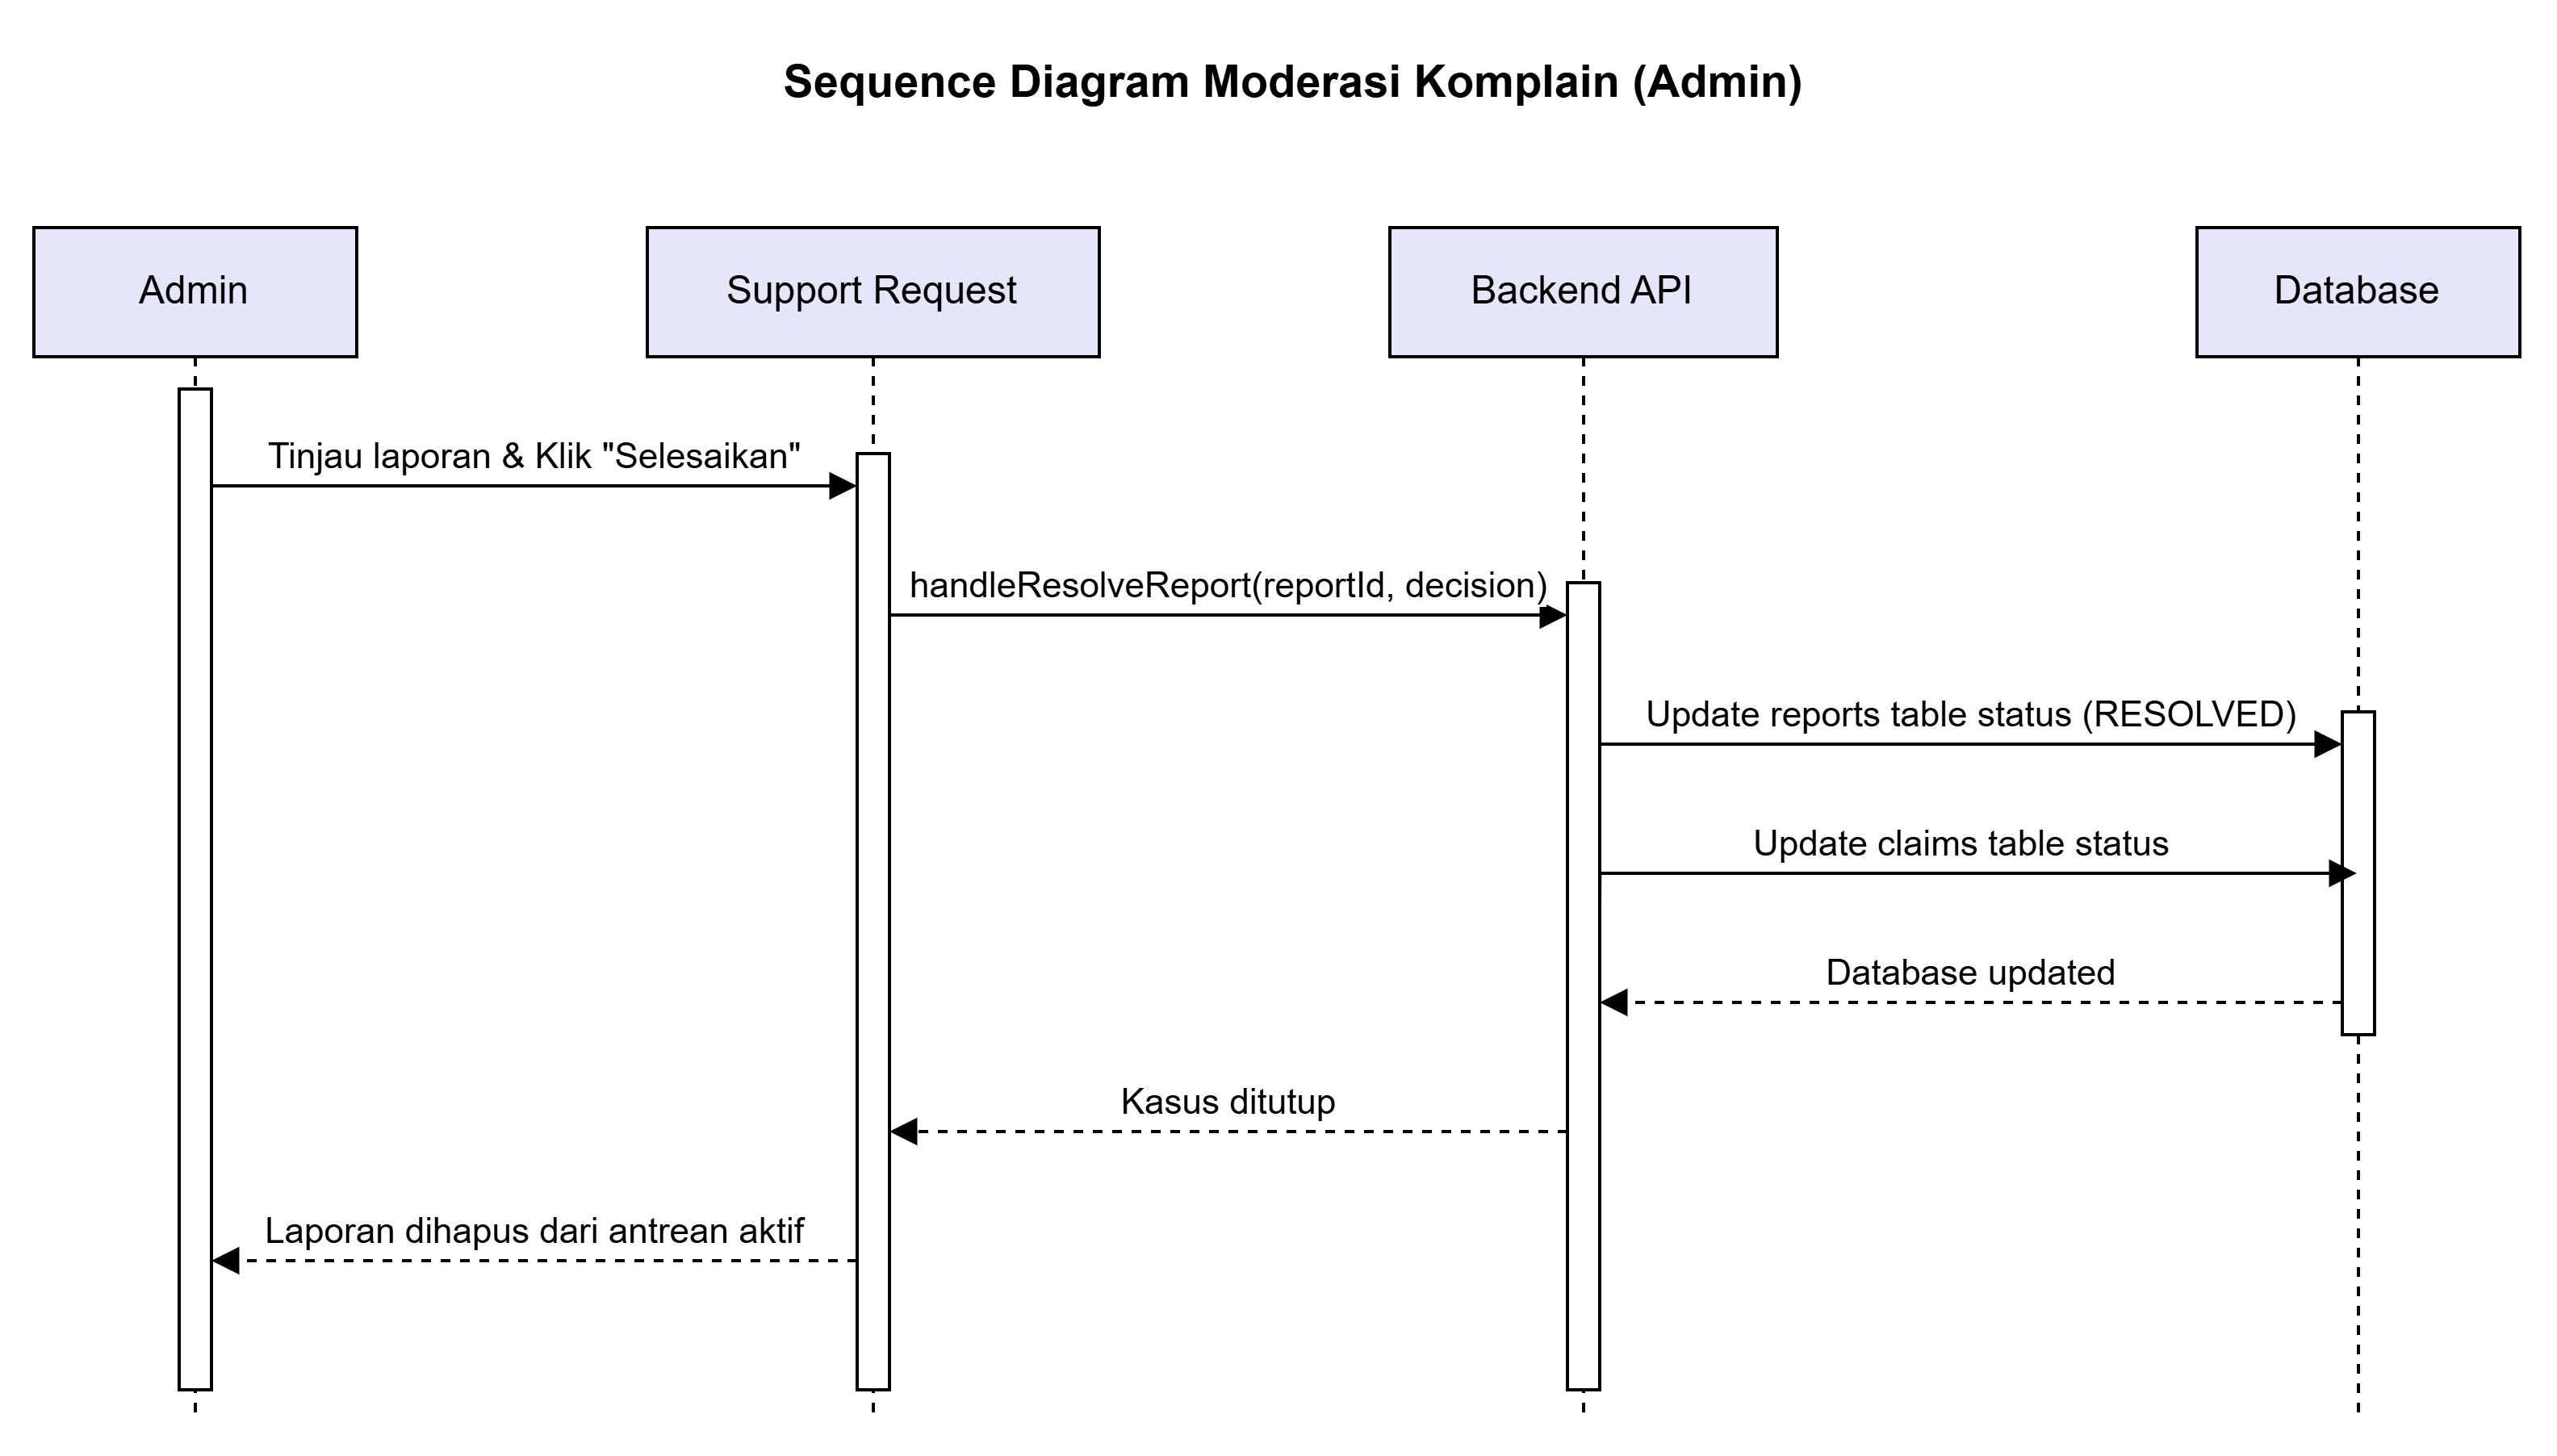
\includegraphics[width=1\textwidth]{image/bab3/sequence/Sequence Diagram Moderasi Komplain (Admin).png}
    \captionsetup{hypcap=false}
    \caption{\textit{Sequence Diagram} Moderasi Komplain (Admin Pengelola)}
    \label{fig:sd-moderasi-admin}
\end{figure}

\textbf{15. \textit{Sequence Diagram} Manajemen Status \textit{Server} (Super Admin)}

Super Admin mengakses \textit{System Config} dan menggeser tuas ``Maintenance Mode'' (ON/OFF). \textit{Backend} menerima \texttt{toggleMaintenance(boolean)} dan memperbarui kunci pengaturan di \textit{Database}. Secara sistemik, tindakan ini akan membatalkan (\textit{invalidate}) seluruh sesi aktif pengguna lain, dan memunculkan tampilan ``mode pemeliharaan'' di seluruh aplikasi.

\begin{figure}[H]
    \centering
    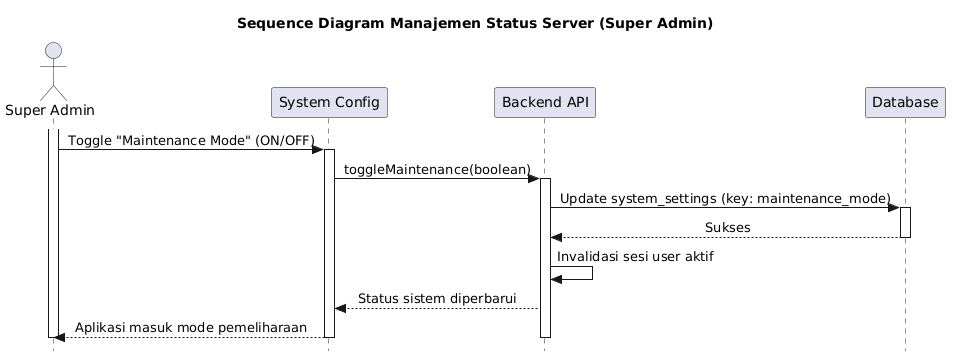
\includegraphics[width=1\textwidth]{image/bab3/sequence/Sequence Diagram Manajemen Status Server (Super Admin).png}
    \captionsetup{hypcap=false}
    \caption{\textit{Sequence Diagram} Manajemen Status \textit{Server} (Super Admin)}
    \label{fig:sd-server-superadmin}
\end{figure}

\noindent Sebagai ringkasan, seluruh \textit{sequence diagram} yang telah dipaparkan di atas dirangkum dalam tabel berikut:

\begin{longtable}{|p{0.6cm}|p{3cm}|p{4.5cm}|p{6cm}|}
    \caption{Daftar dan Spesifikasi \textit{Sequence Diagram} Food AI Rescue}
    \label{tab:ringkasan-sd} \\
    \hline
    \textbf{No} & \textbf{Peran} & \textbf{Nama \textit{Sequence Diagram}} & \textbf{Spesifikasi Pembahasan (Alur Logika)} \\
    \hline
    \endfirsthead
    \hline
    \textbf{No} & \textbf{Peran} & \textbf{Nama \textit{Sequence Diagram}} & \textbf{Spesifikasi Pembahasan (Alur Logika)} \\
    \hline
    \endhead
    \hline
    \multicolumn{4}{r}{\textit{Bersambung ke halaman berikutnya}} \\
    \endfoot
    \hline
    \endlastfoot

    1 & Global / Umum & SD Melakukan \textit{Login} & Menggambarkan alur validasi input kredensial pengguna, pencocokan data di basis data, hingga penerbitan token sesi (JWT) dan pengarahan ke \textit{dashboard} masing-masing peran. \\
    \hline

    2 & Penerima & SD Pencarian \& Klaim Makanan & Membahas proses penelusuran katalog makanan, pemilihan metode pengambilan (mandiri/kurir), pembuatan kode unik, hingga pemotongan stok pada basis data. \\
    \hline

    3 & Penerima & SD Pemberian Ulasan (\textit{Review}) & Menggambarkan alur pengiriman penilaian (bintang) dan media foto terhadap makanan/donatur setelah transaksi berstatus selesai (\textit{completed}). \\
    \hline

    4 & Penerima & SD Pelaporan Masalah (\textit{Report}) & Membahas proses pengiriman detail komplain (beserta bukti foto) yang akan mengubah status transaksi dan memicu notifikasi peringatan ke dasbor Admin. \\
    \hline

    5 & Relawan & SD Penerimaan Misi Pengantaran & Menggambarkan alur pengambilan penugasan logistik dari \textit{Missions Board}, dilengkapi dengan blok alternatif penanganan kegagalan (\textit{race condition}) jika misi ternyata sudah diklaim oleh relawan lain di waktu yang bersamaan. \\
    \hline

    6 & Relawan & SD Validasi Serah Terima (\textit{QR Code} / Manual) & Membahas komunikasi serah terima di mana relawan dapat memindai \textit{QR Code} melalui kamera, atau memasukkan 6-digit kode unik secara manual sebagai cadangan (\textit{fallback}) jika perangkat kamera bermasalah. \\
    \hline

    7 & Relawan & SD Kalkulasi Gamifikasi (Sistem Internal) & Menggambarkan proses sistem berjalan di belakang layar untuk menghitung poin dampak, menaikkan metrik \textit{Experience Point} (XP), dan memperbarui peringkat relawan secara otomatis setelah misi selesai. \\
    \hline

    8 & Donatur Individu & SD Unggah Surplus Makanan \& Verifikasi AI & Membahas alur formulir bertahap (\textit{multi-step form}) di mana donatur menginput data dan foto makanan, yang kemudian divalidasi secara langsung oleh AI (skor keamanan \& alergen) sebelum data disimpan dan dipublikasikan ke katalog. \\
    \hline

    9 & Donatur Individu & SD Konfirmasi Pesanan & Membahas proses Donatur saat menerima notifikasi klaim dari Penerima dan melakukan pembaruan status persetujuan (\textit{Approved/Ready}) pada transaksi. \\
    \hline

    10 & Donatur Individu & SD Dasbor Dampak Sosial (SROI) & Menggambarkan alur sistem saat menarik agregasi data log transaksi dan mengonversinya menjadi grafik visual reduksi emisi karbon (CO\textsubscript{2}) dan penghematan air tanah. \\
    \hline

    11 & Donatur Korporat & SD \textit{Generate} CSR \textit{Copywriter} & Membahas penarikan data transaksi aktual untuk diolah AI menjadi dua versi teks (untuk Donatur dan Penerima) dengan kustomisasi nada dan platform target, disertai fitur pengiriman \textit{request posting} ke akun Penerima. \\
    \hline

    12 & Donatur Korporat & SD Pembuatan Logo \& Rekomendasi Kemasan & Menggambarkan alur pemrosesan AI ganda, di mana sistem menghasilkan gambar logo kemasan, sekaligus menganalisis spesifikasi makanan untuk memberikan rekomendasi material kemasan (misal: anti-air) dan nama vendor di internet. \\
    \hline

    13 & Admin & SD Verifikasi \& Kelola Akun & Menggambarkan alur Admin saat menarik daftar pendaftar baru, memeriksa dokumen identitas, dan mengubah status akun menjadi aktif (terverifikasi) atau ditolak. \\
    \hline

    14 & Admin & SD Moderasi Komplain & Membahas alur resolusi sengketa, di mana Admin meninjau bukti dari Penerima/Relawan dan menetapkan keputusan status final pada log transaksi (basis data). \\
    \hline

    15 & Super Admin & SD Manajemen Status \textit{Server} & Membahas alur pengaktifan \textit{Maintenance Mode}, yang memicu pemutusan sesi (akses) publik dan mengalihkan seluruh lalu lintas pengguna ke halaman pemeliharaan. \\
    \hline

\end{longtable}

% ==============================================================================
\section{Perancangan Antarmuka Pengguna}
% ==============================================================================

Perancangan antarmuka pengguna (\textit{User Interface Design}) merupakan tahapan krusial dalam pengembangan sistem yang bertujuan untuk menjembatani interaksi antara pengguna dengan fungsionalitas di balik layar secara intuitif, efisien, dan estetis. Pada platform \textbf{Food AI Rescue}, antarmuka dirancang berbasis \textit{Progressive Web App} (PWA) menggunakan \textit{framework} React.js dengan TypeScript guna memberikan pengalaman pengguna (\textit{User Experience}/UX) yang sangat responsif, modern, dan dapat diakses dengan lancar lintas perangkat.

Secara visual, desain antarmuka aplikasi Food AI Rescue mengusung konsep premium interaktif dengan gaya tembus pandang (\textit{Glassmorphism}) yang dipadukan dengan pesona latar belakang \textit{mesh gradients}. Guna mempermudah navigasi dan interaksi, antarmuka ini juga dibekali dengan elemen visual dinamis seperti animasi alur operasional (\textit{Roadmap}) dan \textit{cursor follower} khusus yang dirancang untuk memandu pengguna baru dalam menjelajahi ekosistem aplikasi.

Selain itu, tata letak setiap layar dirancang secara eksklusif mengikuti arsitektur hak akses (\textit{Role-Based Access Control}), sehingga masing-masing pengguna (Donatur Individu, Donatur Korporat, Penerima, Relawan, Admin, dan Super Admin) mendapatkan menu dan dasbor yang relevan dengan tugas mereka, mulai dari panel verifikasi keamanan pangan AI, pelacakan rute navigasi \textit{booking}, \textit{leaderboard} gamifikasi relawan, hingga visualisasi Dasbor Dampak Sosial (SROI).

\subsection{Antarmuka Pemasaran Publik dan Autentikasi}

% Tambahkan gambar dan penjelasan antarmuka halaman publik dan login di sini

\subsection{Antarmuka Dasbor Donatur (Individu dan Korporat)}

% Tambahkan gambar dan penjelasan antarmuka dasbor donatur di sini

\subsection{Antarmuka Dasbor Penerima Donasi}

% Tambahkan gambar dan penjelasan antarmuka dasbor penerima di sini

\subsection{Antarmuka Dasbor Relawan}

% Tambahkan gambar dan penjelasan antarmuka dasbor relawan di sini

\subsection{Antarmuka Dasbor Admin dan Super Admin}

% Tambahkan gambar dan penjelasan antarmuka dasbor admin dan super admin di sini

% ==============================================================================
\section{Kebutuhan Perangkat Keras dan Perangkat Lunak}
% ==============================================================================

Guna menunjang keberhasilan rancang bangun platform \textit{Food AI Rescue}---baik pada fase rekayasa lokal maupun penerapan di tingkat produksi (\textit{deployment})---diperlukan spesifikasi infrastruktur teknologi yang terukur dan andal. Subbab ini merincikan daftar kebutuhan spesifikasi minimum perangkat keras (\textit{hardware}) dan perangkat lunak (\textit{software}) yang berfungsi sebagai lingkungan operasional (\textit{environment}) bagi sistem basis data, peladen \textit{backend}, integrasi API \textit{Machine Learning}, hingga perangkat akses akhir yang digunakan oleh pengguna di lapangan.

\subsection{Pengembangan Sistem}
\label{subsec:kebutuhan-pengembangan}

Kebutuhan perangkat keras (\textit{hardware}) yang digunakan oleh penulis dalam proses pembuatan dan pengembangan platform \textit{Food AI Rescue} adalah sebagai berikut:

\begin{longtable}{|p{0.5cm}|p{2.8cm}|p{5.5cm}|p{4.8cm}|}
    \caption{Kebutuhan Perangkat Keras (\textit{Hardware}) Pengembangan}
    \label{tab:hardware-dev} \\
    \hline
    \textbf{No} & \textbf{Perangkat} & \textbf{Fungsi} & \textbf{Spesifikasi} \\
    \hline
    \endfirsthead
    \hline
    \textbf{No} & \textbf{Perangkat} & \textbf{Fungsi} & \textbf{Spesifikasi} \\
    \hline
    \endhead
    \hline
    \multicolumn{4}{r}{\textit{Bersambung ke halaman berikutnya}} \\
    \endfoot
    \hline
    \endlastfoot
    1 & Laptop & Digunakan sebagai \textit{workstation} utama untuk mengembangkan dan menjalankan program atau aplikasi. & Lenovo IdeaPad 3 14IAU7 \\
    \hline
    2 & Prosesor & Berfungsi memproses instruksi komputasi dan menjalankan arsitektur aplikasi \textit{client-server}. & 12th Gen Intel(R) Core(TM) i3-1215U (1.20 GHz) \\
    \hline
    3 & RAM & Memori sementara yang mendukung kinerja sistem saat mengompilasi kode dan mengolah data secara lokal. & 8 GB DDR4 \\
    \hline
    4 & Penyimpanan & Menyimpan sistem operasi, data \textit{database}, dan \textit{source code} proyek agar dapat diakses dengan cepat. & SSD 512 GB \\
    \hline
    5 & Monitor & Menampilkan antarmuka kode serta pratinjau \textit{output} dari \textit{Progressive Web App} (PWA) yang dibangun. & 14 inch, resolusi 1920$\times$1080 (\textit{Full HD}) \\
    \hline
    6 & \textit{Keyboard} & Alat \textit{input} untuk mengetik skrip kode pemrograman dan memberikan perintah operasional ke komputer. & -- \\
    \hline
    7 & Internet & Sarana krusial untuk mengakses dokumentasi, mengunduh \textit{library} NPM, serta mengakses \textit{Google Gemini API}. & -- \\
    \hline
\end{longtable}

Perangkat lunak (\textit{software}) meliputi sistem operasi, bahasa pemrograman, \textit{framework}, dan alat desain yang digunakan oleh penulis dalam merancang hingga membangun aplikasi \textit{Food AI Rescue} di lingkungan lokal. Rinciannya adalah sebagai berikut:

\begin{longtable}{|p{0.5cm}|p{3.5cm}|p{5cm}|p{4.5cm}|}
    \caption{Kebutuhan Perangkat Lunak (\textit{Software}) Pengembangan}
    \label{tab:software-dev} \\
    \hline
    \textbf{No} & \textbf{Perangkat} & \textbf{Fungsi} & \textbf{Spesifikasi} \\
    \hline
    \endfirsthead
    \hline
    \textbf{No} & \textbf{Perangkat} & \textbf{Fungsi} & \textbf{Spesifikasi} \\
    \hline
    \endhead
    \hline
    \multicolumn{4}{r}{\textit{Bersambung ke halaman berikutnya}} \\
    \endfoot
    \hline
    \endlastfoot
    1 & Sistem Operasi & Menyediakan platform dasar untuk menjalankan dan mengelola seluruh aplikasi pengembangan. & Windows 11 Home Single Language \\
    \hline
    2 & Lingkungan \textit{Backend} (Node.js \& Express.js) & Lingkungan eksekusi utama dan \textit{framework} API untuk memproses logika bisnis sistem di sisi server lokal. & Node.js / Express (v5.x) \\
    \hline
    3 & Lingkungan \textit{Frontend} (React.ts \& Vite) & \textit{Framework} berbasis komponen dan \textit{build-tool} untuk merancang antarmuka pengguna (UI) yang reaktif. & React.js (v19) dengan TypeScript \\
    \hline
    4 & XAMPP / Laragon & Perangkat lunak \textit{web server} lokal yang menyediakan layanan modul pangkalan data. & Modul MySQL \\
    \hline
    5 & MySQL & Sistem manajemen basis data (RDBMS) utama untuk menyimpan dan mengelola rekam jejak data aplikasi. & MySQL (MariaDB) versi 10.4.32 \\
    \hline
    6 & VSCode & \textit{Text editor} utama yang digunakan untuk penulisan \textit{source code} pengembangan aplikasi. & Version 1.102.2 \\
    \hline
    7 & Google Chrome & Peramban utama untuk menguji \textit{debugging} dan menjalankan aplikasi web secara lokal (\textit{localhost}). & Version 138.0.7204.168 \\
    \hline
    8 & Figma & Alat desain antarmuka pengguna untuk membuat prototipe, \textit{wireframe}, dan merancang gaya \textit{Glassmorphism}. & Versi berbasis web \\
    \hline
    9 & Draw.io \& PlantUML & Alat bantu visualisasi untuk merancang berbagai pemodelan \textit{Unified Modeling Language} (UML) dan BPMN. & Versi berbasis web \\
    \hline
    10 & Google Gemini Vision API & Layanan Kecerdasan Buatan (AI) pihak ketiga untuk fitur verifikasi kelayakan makanan dan konten generatif. & API / \textit{Cloud Service} \\
    \hline
\end{longtable}

\subsection{Implementasi Sistem}
\label{subsec:kebutuhan-implementasi}

Agar platform \textit{Food AI Rescue} dapat dieksekusi dan dikembangkan secara optimal pada perangkat komputasi lain, dibutuhkan spesifikasi minimal untuk perangkat keras (\textit{hardware}) maupun perangkat lunak (\textit{software}) sebagai berikut:

\begin{longtable}{|p{0.5cm}|p{2.8cm}|p{5.5cm}|p{4.8cm}|}
    \caption{Kebutuhan Perangkat Keras dan Perangkat Lunak (Minimal) dalam Pengerjaan TA}
    \label{tab:hardware-impl} \\
    \hline
    \textbf{No} & \textbf{Perangkat} & \textbf{Fungsi} & \textbf{Spesifikasi (Minimal)} \\
    \hline
    \endfirsthead
    \hline
    \textbf{No} & \textbf{Perangkat} & \textbf{Fungsi} & \textbf{Spesifikasi (Minimal)} \\
    \hline
    \endhead
    \hline
    \multicolumn{4}{r}{\textit{Bersambung ke halaman berikutnya}} \\
    \endfoot
    \hline
    \endlastfoot
    1 & Laptop/PC & Digunakan sebagai \textit{workstation} utama untuk merancang, memprogram, dan menjalankan arsitektur aplikasi \textit{client-server}. & Prosesor Intel Core i3 (atau setara) ke atas \\
    \hline
    2 & RAM & Menjaga stabilitas kinerja sistem komputasi saat mengeksekusi server lokal dan memproses kompilasi kode. & 8 GB \\
    \hline
    3 & Sistem Operasi & Menyediakan lingkungan dasar yang mendukung jalannya \textit{tools} pengembangan aplikasi berbasis web. & Windows 10/11, macOS, atau Linux \\
    \hline
    4 & VSCode & Penyunting kode (\textit{text editor}) utama untuk menulis, mengelola, dan melakukan \textit{debugging} pada \textit{source code frontend} maupun \textit{backend}. & Versi 1.59.x atau yang lebih baru \\
    \hline
    5 & Node.js & Lingkungan eksekusi utama untuk menjalankan kerangka kerja server \textit{backend} (Express.js), \textit{frontend} (React), dan integrasi API. & Versi 18.x LTS atau yang lebih tinggi \\
    \hline
\end{longtable}

\chapter{IMPLEMENTASI DAN PENGUJIAN}
\label{chapter:IMPLEMENTASI DAN PENGUJIAN}
\section{Implementasi}

\subsection{Struktur Antarmuka dan Modul Sistem}
\begin{enumerate}[label=\arabic*.]
    \item Modul Pemasaran \& Publik: menangani antarmuka awal dan etalase informasi aplikasi sebelum pengguna masuk:
    \begin{enumerate}[label=\alph*.]
        \item \texttt{LandingPage.tsx}: Halaman beranda interaktif dengan animasi roadmap dan efek kursor.
    \end{enumerate}
    
    \item Modul Autentikasi \& Manajemen Akun: menangani proses masuk, pendaftaran, serta pengaturan profil pengguna:
    \begin{enumerate}[label=\alph*.]
        \item \texttt{Login.tsx}, \texttt{Register.tsx}: Form login dan registrasi peran akun (Donatur, Penerima, Relawan).
        \item \texttt{ForgotPassword.tsx}: Antarmuka pemulihan kata sandi pengguna.
        \item \texttt{index.tsx}, \texttt{ProfileHeader.tsx}: Dashboard profil dan ringkasan gamifikasi level.
        \item \texttt{AIApiManagement.tsx}: Manajemen input Gemini API Key pribadi untuk membuka fitur AI lanjutan.
        \item \texttt{EditProfile.tsx}, \texttt{SecuritySettings.tsx}: Form pembaruan biodata dan keamanan akun.
        \item \texttt{AddressList.tsx}: Pengaturan titik koordinat alamat logistik.
        \item \texttt{ClaimHistory.tsx}, \texttt{ClaimHistoryDetail.tsx}: Riwayat klaim donasi makanan yang telah dilakukan pengguna.
        \item \texttt{PointHistory.tsx}, \texttt{GamificationSummary.tsx}: Catatan riwayat poin dan pencapaian gamifikasi pengguna.
        \item \texttt{FaqSection.tsx}, \texttt{SavedItems.tsx}: Pusat bantuan in-app dan daftar donasi yang disimpan.
    \end{enumerate}
    
    \item Modul Manajemen Donasi \& Gudang Makanan (Provider): digunakan oleh donatur untuk mengelola stok, donasi, dan riwayat pesanan:
    \begin{enumerate}[label=\alph*.]
        \item \texttt{index.tsx}: Dashboard utama logistik donatur.
        \item \texttt{Inventory.tsx}, \texttt{InventoryNavigation.tsx}: Menampilkan daftar makanan yang sedang tayang di platform.
        \item \texttt{QualityCheckInventoryInput.tsx}: Form unggah donasi pangan dengan fitur Live Camera.
        \item \texttt{QualityCheckInventory.tsx}: Memproses audit kelayakan donasi makanan menggunakan AI Gemini.
        \item \texttt{CorporateAIWidgets.tsx}: Widget AI khusus (Kreator Resep, CSR Writer) untuk donatur korporat.
        \item \texttt{ImpactWidget.tsx}, \texttt{QuickActions.tsx}, \texttt{StatsGrid.tsx}, \texttt{RankCard.tsx}: Kumpulan widget statistik pada dashboard donatur.
        \item \texttt{StockManager.tsx}, \texttt{StockFilters.tsx}, \texttt{ProductDetailModal.tsx}: Manajemen daftar stok, filter, dan detail donasi.
        \item \texttt{OrderList/index.tsx}, \texttt{OrderItemCard.tsx}: Daftar pesanan atau klaim masuk dari penerima.
        \item \texttt{OrderDetail/index.tsx}, \texttt{CourierInfo.tsx}, \texttt{ReceiverInfo.tsx}, \texttt{TimelineDetails.tsx}: Detail proses logistik dan status pengiriman pesanan donasi.
        \item \texttt{HistoryList/index.tsx}, \texttt{HistoryItemCard.tsx}, \texttt{HistoryDetail/index.tsx}, \texttt{Timeline.tsx}: Daftar dan detail riwayat donasi yang telah selesai (riwayat logistik).
        \item \texttt{Reports/index.tsx}, \texttt{ReportDetailModal.tsx}: Manajemen laporan dan komplain dari pengguna terkait donasi.
        \item \texttt{Reviews/index.tsx}, \texttt{ReviewItemCard.tsx}: Menampilkan ulasan dan rating dari penerima donasi.
    \end{enumerate}

    \item Modul Radar Penerima (Receiver): menangani eksplorasi donasi makanan terdekat dan pusat permintaan bagi penerima:
    \begin{enumerate}[label=\alph*.]
        \item \texttt{index.tsx}: Dashboard eksplorasi utama bagi panti asuhan atau individu penerima manfaat.
        \item \texttt{FoodList.tsx}, \texttt{FoodDetail.tsx}: Menampilkan katalog visual donasi terdekat beserta jarak radius dan detailnya.
        \item \texttt{AIVerificationCard.tsx}: Komponen stempel hijau jaminan mutu bahwa donasi telah diaudit oleh AI.
        \item \texttt{StoreIcon.tsx}: Representasi visual ikon toko atau titik donatur di peta.
        \item \texttt{RequestManager.tsx}: Fasilitas bagi penerima untuk mempublikasikan permintaan donasi spesifik ke publik donatur.
    \end{enumerate}

    \item Modul Operasional Kurir \& Gamifikasi (Volunteer): digunakan oleh relawan untuk mengambil misi penjemputan dan melacak metrik operasional:
    \begin{enumerate}[label=\alph*.]
        \item \texttt{index.tsx}, \texttt{StatsDashboard.tsx}: Dashboard relawan yang memuat statistik harian (jarak tempuh dan poin).
        \item \texttt{MissionList.tsx}: Menampilkan daftar antrean misi penjemputan donasi yang tersedia untuk diambil.
        \item \texttt{MissionDetail.tsx}: Detail eksekusi misi yang mencakup manifest muatan, peta rute Google Maps 3-titik, fitur chat WA instan, dan QR Code Pickup.
        \item \texttt{HistoryList.tsx}: Log riwayat misi logistik pengantaran yang pernah diselesaikan.
        \item \texttt{Leaderboard.tsx}: Papan klasemen persaingan poin antar relawan.
    \end{enumerate}

    \item Modul Konfigurasi \& Intervensi Pusat (Admin): memiliki akses untuk mengelola gamifikasi, konten, logistik global, dan moderasi pengguna:
    \begin{enumerate}[label=\alph*.]
        \item \texttt{index.tsx}, \texttt{Overview.tsx}: Dashboard utama pengawas super-admin.
        \item \texttt{SystemConfig.tsx}, \texttt{LogViewer.tsx}: Pengaturan variabel sistem dan pemantauan aliran log teknis.
        \item \texttt{AdminList.tsx}, \texttt{Impact.tsx}: Manajemen data pengguna admin dan kalkulasi SROI (Social Return on Investment).
        \item \texttt{RanksManagement.tsx}: Mengelola level dan poin gamifikasi dengan antarmuka drag-and-drop.
        \item \texttt{Distribution.tsx}, \texttt{Moderation.tsx}: Pelacakan riwayat distribusi logistik lintas pengguna dan pemrosesan sengketa/komplain.
        \item \texttt{ContentCMS.tsx}: Sistem manajemen konten FAQ dan SOP menggunakan editor markdown.
        \item \texttt{Communication/index.tsx}, \texttt{BroadcastHistory.tsx}, \texttt{ComposeMessage.tsx}: Mengelola pengiriman siaran pesan massal dari admin ke perangkat pengguna.
        \item \texttt{Community/index.tsx}, \texttt{UserList.tsx}, \texttt{VerificationModal.tsx}: Manajemen daftar pengguna dan verifikasi keabsahan institusi yayasan/restoran.
        \item \texttt{Community/BadgeCatalog.tsx}, \texttt{BadgeModal.tsx}: Mengelola pembuatan katalog medali/badge pencapaian untuk pengguna.
    \end{enumerate}

    \item Modul Penunjang Bersama (Shared Components): berisi elemen antarmuka, utilitas AI, dan pop-up yang dipakai lintas modul di atas:
    \begin{enumerate}[label=\alph*.]
        \item \texttt{DesktopLayout.tsx}, \texttt{Sidebar.tsx}, \texttt{TopAppBar.tsx}: Kerangka dan kerangka struktur navigasi utama aplikasi.
        \item \texttt{CSRWriterEditor.tsx}, \texttt{EcoPackagingEditor.tsx}: Antarmuka editor cerdas bantuan AI.
        \item \texttt{KitchenScanner.tsx}: Modul integrasi pemindai kamera untuk kelayakan fasilitas dapur.
        \item \texttt{AddressWarningModal.tsx}, \texttt{VerificationPendingModal.tsx}, \texttt{SuccessClaimSplash.tsx}: Kumpulan modal peringatan dan notifikasi splash (pop-up sistem).
        \item \texttt{Button.tsx}, \texttt{Input.tsx}, \texttt{CounterUp.tsx}: Blok pembangun dasar UI sistem (komponen form, tombol, dan animasi numerik).
    \end{enumerate}
\end{enumerate}

\subsection{Hak Akses Pengguna (\textit{Role-Based Access Control})}

Kapasitas jumlah pengguna pada platform FoodAI Rescue tidak dibatasi secara kuantitas, namun kewenangannya diklasifikasikan ke dalam 6 (enam) jenis peran yang berbeda untuk menjaga keamanan dan privasi data. Keenam jenis pengguna tersebut adalah:

\begin{enumerate}[label=\arabic*.]
    \item \textbf{Donatur Individu}: Pengguna skala rumah tangga atau usaha mikro yang dapat mengunggah donasi makanan sisa, memantau Dasbor Dampak Sosial (SROI), serta menggunakan AI \textit{Quality Verification} ("Polisi Pangan") untuk memvalidasi kelayakan makanan secara mandiri.
    \item \textbf{Donatur Korporat}: Pengguna dari sektor industri komersial (HORECA) yang memiliki fungsionalitas serupa dengan donatur individu, ditambah hak akses eksklusif terhadap modul AI Generatif (\textit{Eco Packaging Editor} dan \textit{CSR Copywriter}) guna memproduksi materi kampanye keberlanjutan perusahaan.
    \item \textbf{Penerima (Mitra Penerima)}: Kelompok masyarakat rentan atau fasilitas sosial yang memiliki akses untuk mencari ketersediaan makanan di radar peta, melakukan klaim (\textit{booking}) pesanan, serta memberikan ulasan pasca-donasi.
    \item \textbf{Relawan (Kurir Logistik)}: Pasukan sukarela yang bertugas mengambil misi penjemputan dan pengantaran makanan. Relawan berinteraksi dengan sistem menggunakan kewajiban pindai (\textit{mandatory scan}) Kode QR saat serah terima, dan berhak mendapatkan poin XP pada sistem gamifikasi.
    \item \textbf{Admin Pengelola}: Pengelola sistem operasional yang bertugas memverifikasi pendaftaran akun, menangani laporan keluhan pengguna, memantau Dasbor Statistik, serta menyesuaikan parameter \textit{Prompt Engineering} pada AI.
    \item \textbf{Super Admin}: Tim pengembang (IT) yang memiliki kedaulatan penuh terhadap infrastruktur \textit{backend}, bertugas melakukan pemeliharaan server (mengaktifkan \textit{maintenance mode}), serta memonitor jejak \textit{log} sistem secara keseluruhan.
\end{enumerate}

\subsection{Langkah Instalasi dan Konfigurasi Sistem}
Untuk menginstal dan menjalankan platform FoodAI Rescue secara lokal (\textit{localhost}), langkah-langkah berikut dapat diikuti:

\begin{enumerate}[label=\arabic*.]
    \item Unduh (\textit{clone}) \textit{source code} aplikasi dari repositori GitHub dan buka proyek tersebut menggunakan IDE (misalnya Visual Studio Code).
    \item Siapkan dan aktifkan layanan basis data MySQL melalui panel kontrol XAMPP atau Laragon.
    \item Jalankan server \textit{backend} (arahkan terminal ke folder \texttt{server} lalu ketik \texttt{npm run dev}) dan berikan izin saat muncul peringatan untuk melakukan migrasi \textit{database} secara otomatis.
    \item Lakukan konfigurasi akun utama melalui terminal dengan memasukkan \textit{email} dan \textit{password} untuk \textit{Super Admin}, lalu \textit{scan} QR Code untuk menautkan layanan \textit{gateway} WhatsApp.
    \item Jalankan server \textit{frontend} (buka terminal baru pada direktori utama lalu ketik \texttt{npm run dev}).
    \item Akses dan jalankan sistem melalui peramban (\textit{web browser}) pada alamat \url{http://localhost:3000/}.
\end{enumerate}

\subsection{User Manual}

\textbf{A. Akses Pengguna}

\subsubsection{Proses Registrasi Pengguna}
Langkah-langkah untuk melakukan pendaftaran akun baru pada platform Food AI Rescue adalah sebagai berikut:
\begin{enumerate}[label=\arabic*.]
    \item Akses halaman utama aplikasi dan tekan tombol \textbf{Daftar Gratis}.
    \item Pilih peran (\textit{role}) pengguna yang sesuai dengan entitas Anda, misalnya Donatur, Penerima, atau Relawan.
    \item Isi kelengkapan formulir pendaftaran akun (seperti nama, email, dan kata sandi), lalu tekan \textbf{Daftar}.
    \item Masukkan kode OTP (\textit{One-Time Password}) yang dikirimkan ke alamat email Anda untuk menyelesaikan proses verifikasi.
\end{enumerate}

\begin{figure}[H]
    \centering
    \includegraphics[width=\linewidth]{image/bab4/UserManual/Registrasi/1-Landing.png}
    \caption{Halaman Utama Aplikasi}
\end{figure}

\begin{figure}[H]
    \centering
    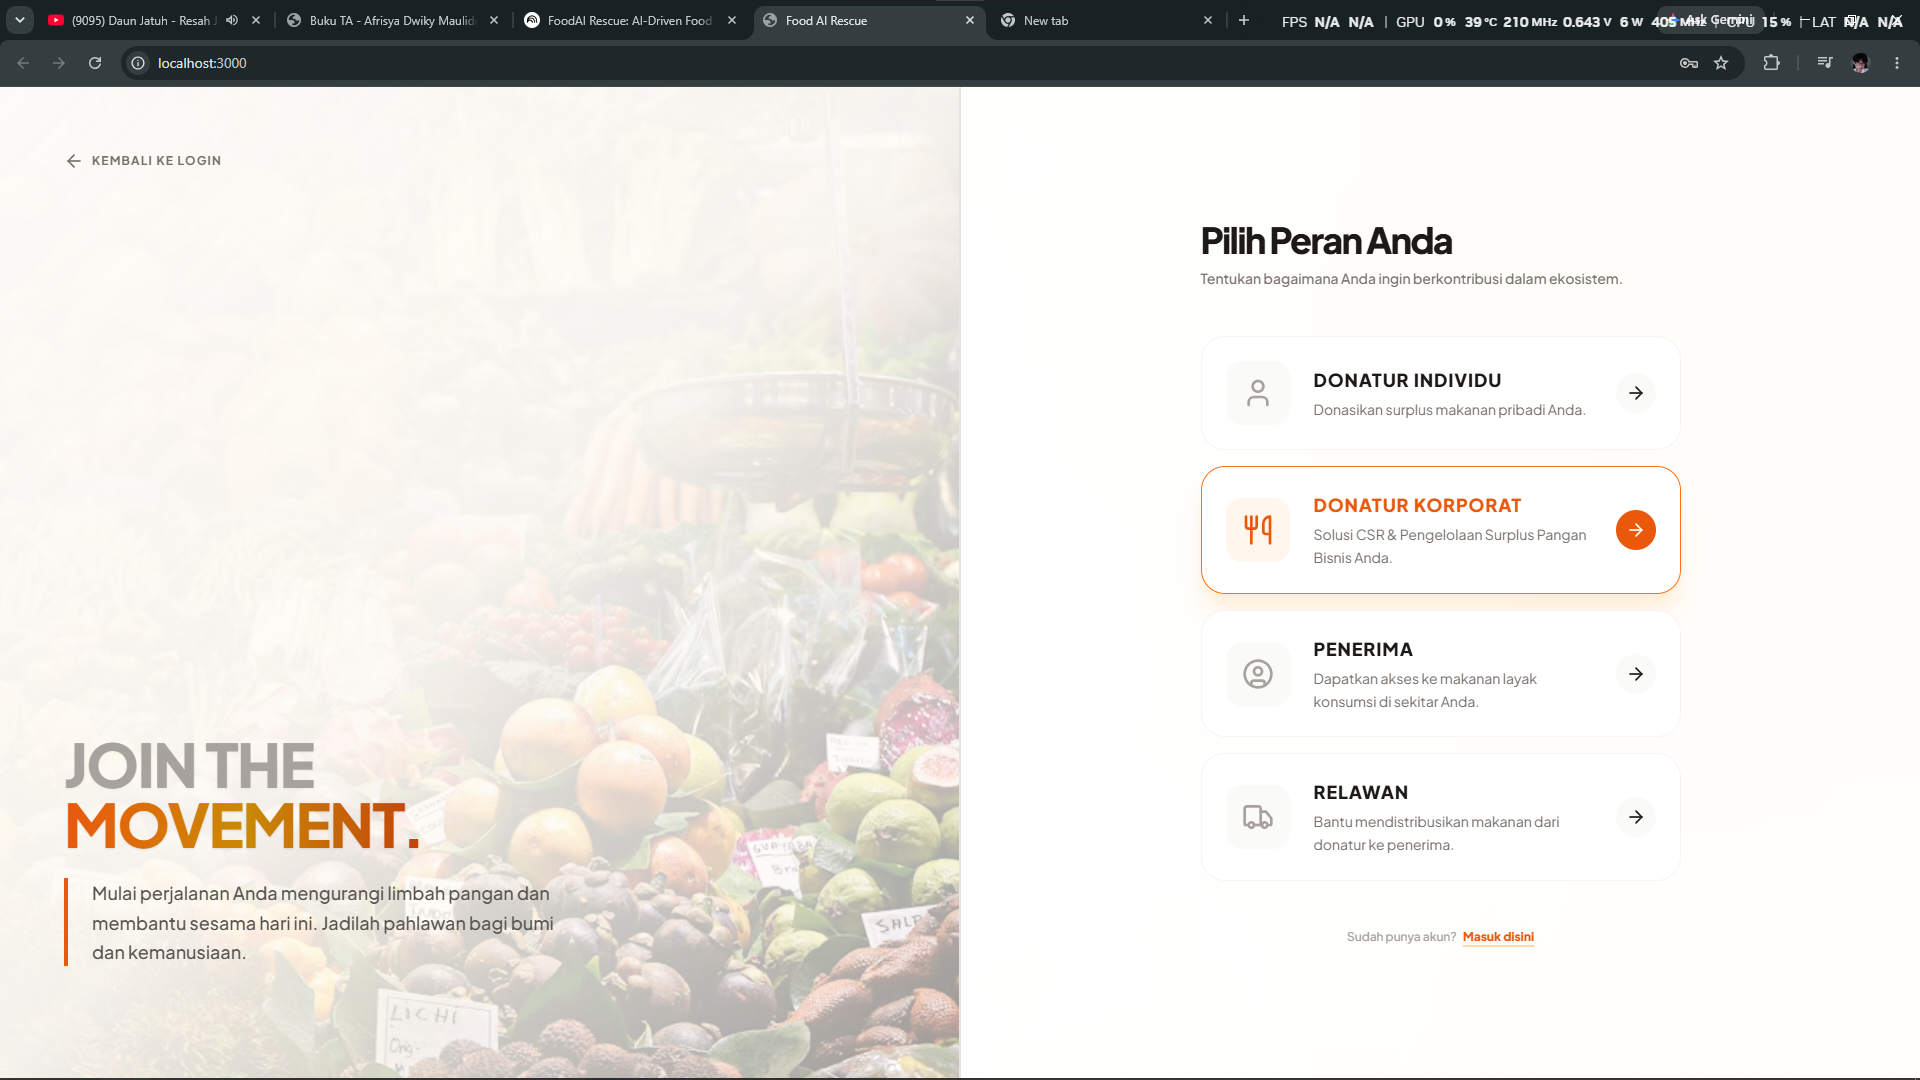
\includegraphics[width=\linewidth]{image/bab4/UserManual/Registrasi/2-PilihPeran.png}
    \caption{Halaman Pemilihan Peran}
\end{figure}



\begin{figure}[H]
    \centering
    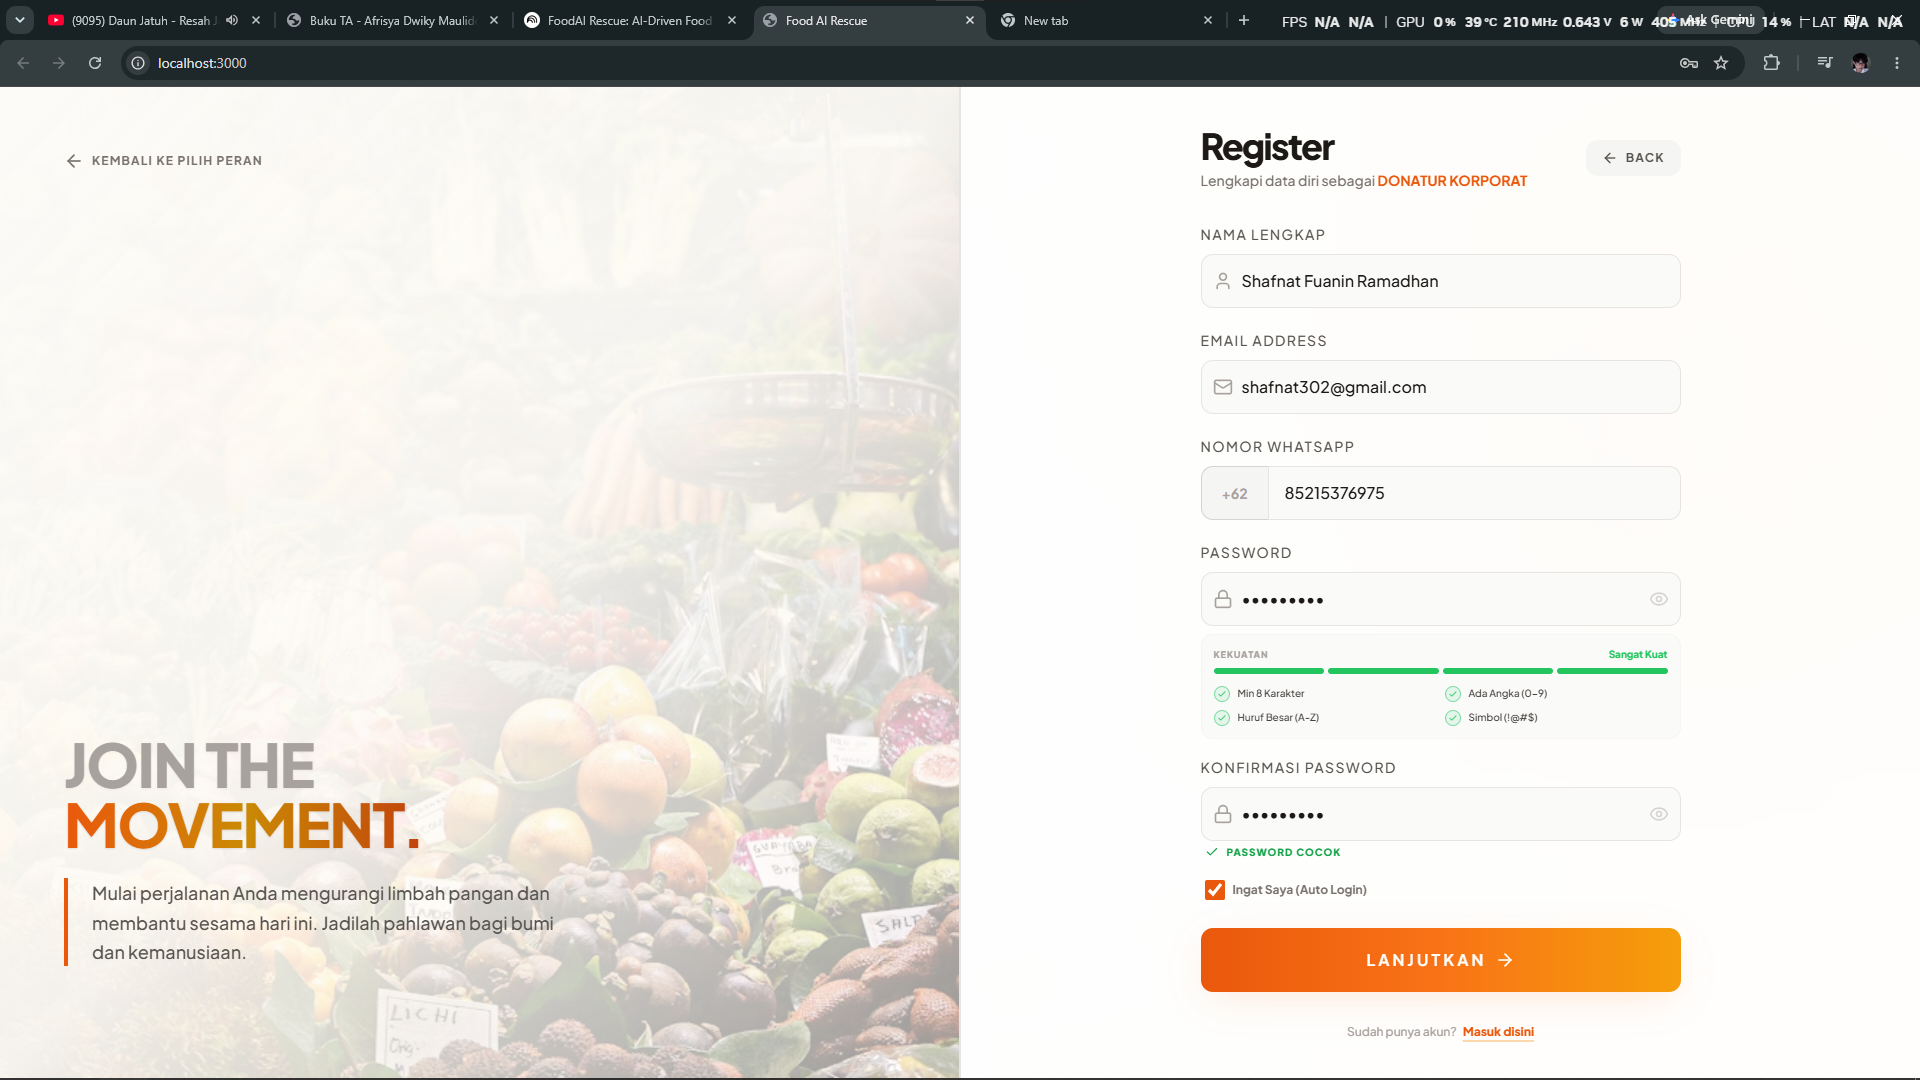
\includegraphics[width=\linewidth]{image/bab4/UserManual/Registrasi/3-Register.png}
    \caption{Formulir Registrasi}
\end{figure}

\begin{figure}[H]
    \centering
    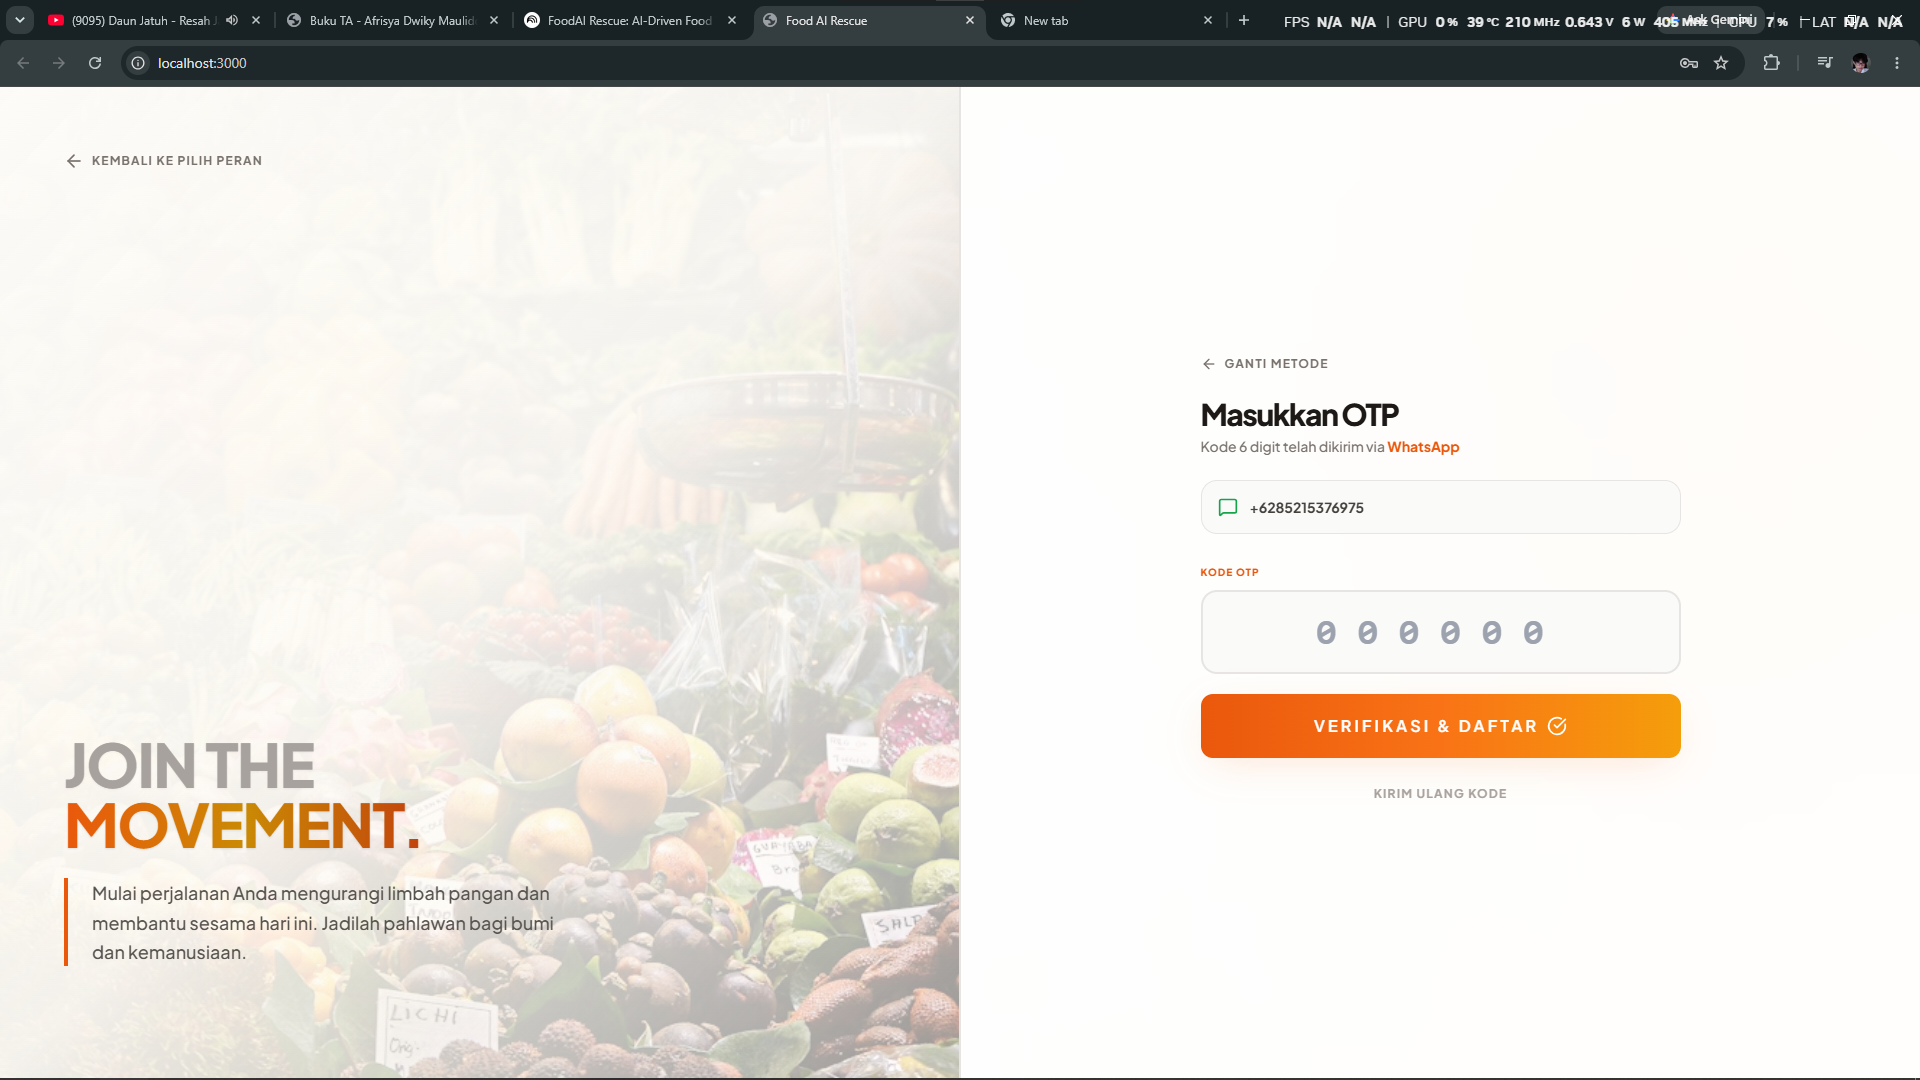
\includegraphics[width=\linewidth]{image/bab4/UserManual/Registrasi/4-OTP.png}
    \caption{Verifikasi OTP}
\end{figure}



\subsubsection{Proses Login Pengguna}
Langkah-langkah untuk masuk ke dalam dasbor sistem:
\begin{enumerate}[label=\arabic*.]
    \item Akses halaman utama dan tekan tombol \textbf{Masuk}.
    \item Masukkan kredensial email dan kata sandi yang telah terdaftar, kemudian tekan tombol \textbf{Masuk}.
\end{enumerate}

\begin{figure}[H]
    \centering
    \includegraphics[width=\linewidth]{image/bab4/UserManual/Login/1-Landing.png}
    \caption{Halaman Utama Aplikasi}
\end{figure}

\begin{figure}[H]
    \centering
    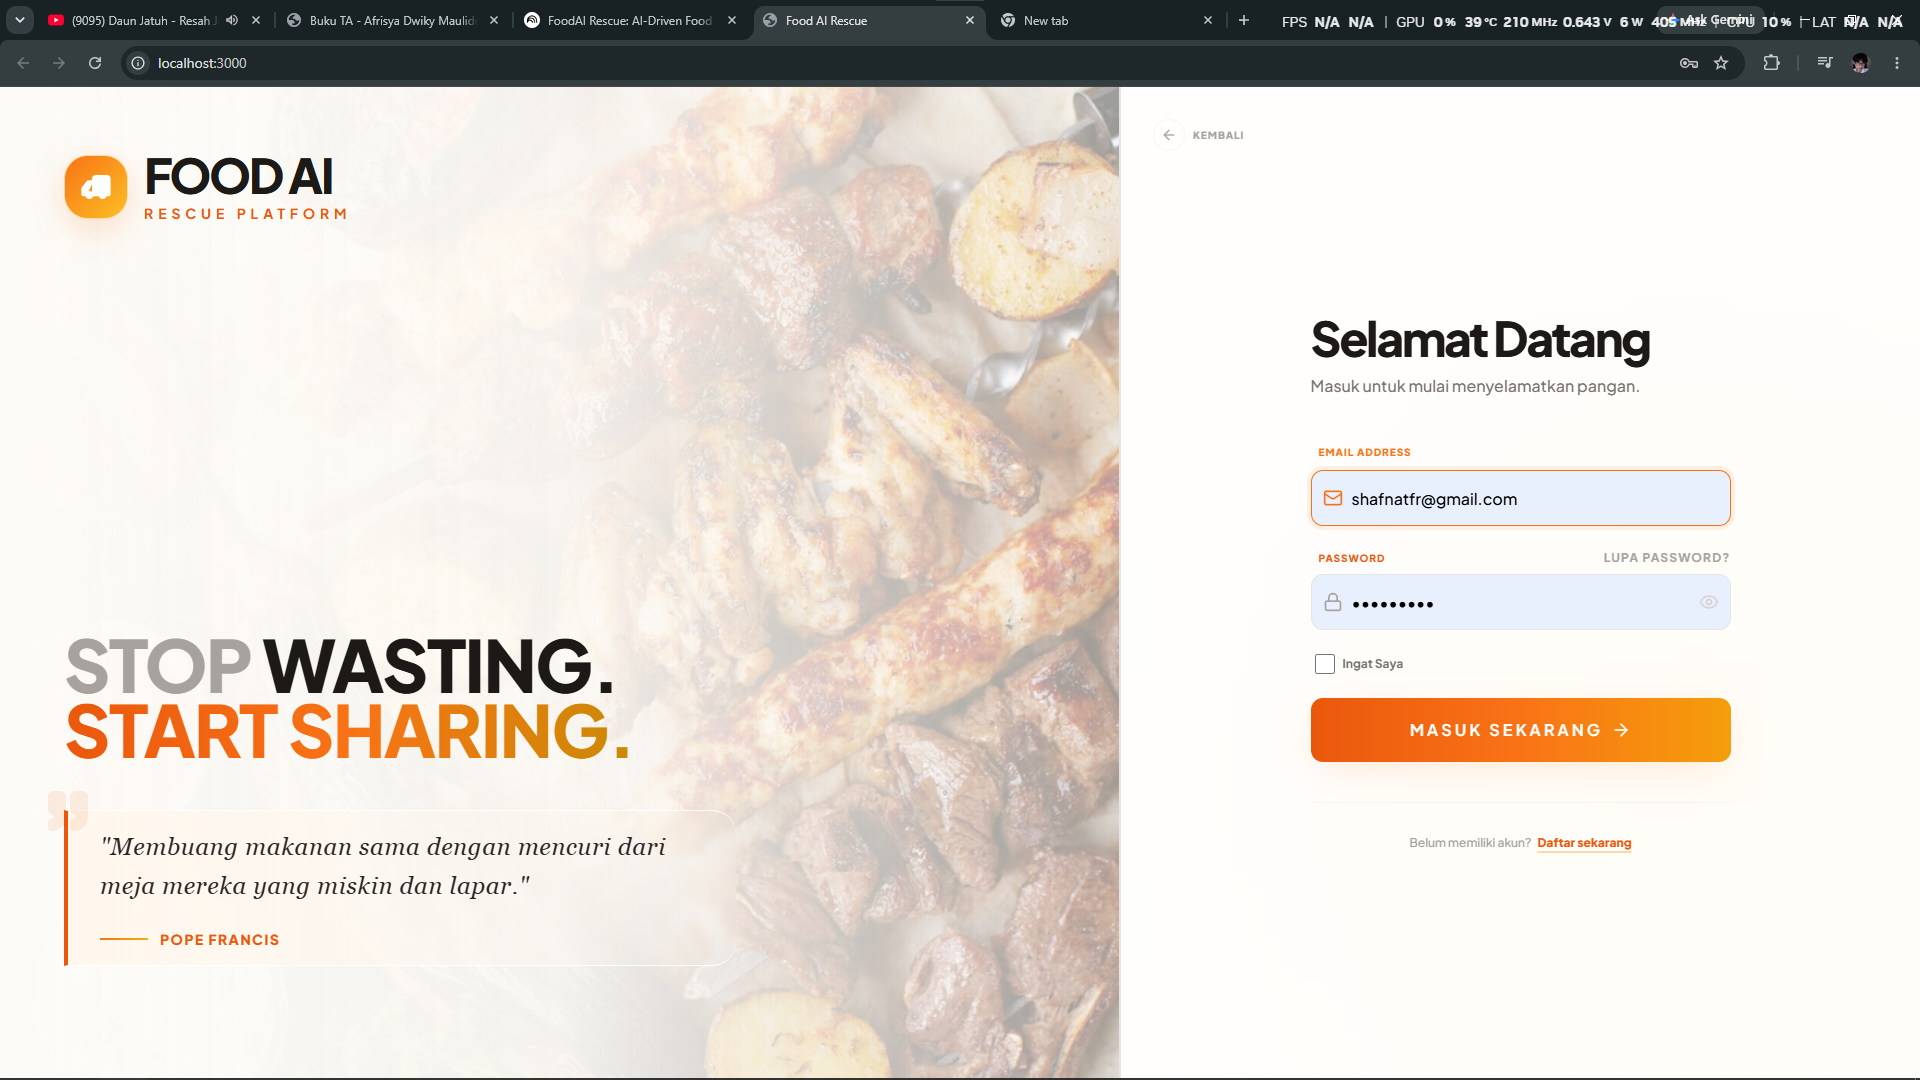
\includegraphics[width=\linewidth]{image/bab4/UserManual/Login/2-Login.png}
    \caption{Halaman \textit{Login}}
\end{figure}



\textbf{B. Pengguna Donatur (Penyedia Makanan)}

\subsubsection{Proses Input Donasi Makanan}
Langkah-langkah untuk mendata surplus makanan:
\begin{enumerate}[label=\arabic*.]
    \item Buka menu \textbf{Manajemen Stok} pada dasbor Donatur, lalu tekan \textbf{Tambah Donasi}.
    \item Isi rincian makanan yang akan didonasikan dan unggah fotonya.
    \item Sistem (Polisi Pangan) akan menampilkan hasil audit kualitas berbasis AI. Jika dinyatakan aman, tekan publikasikan donasi.
\end{enumerate}

\begin{figure}[H]
    \centering
    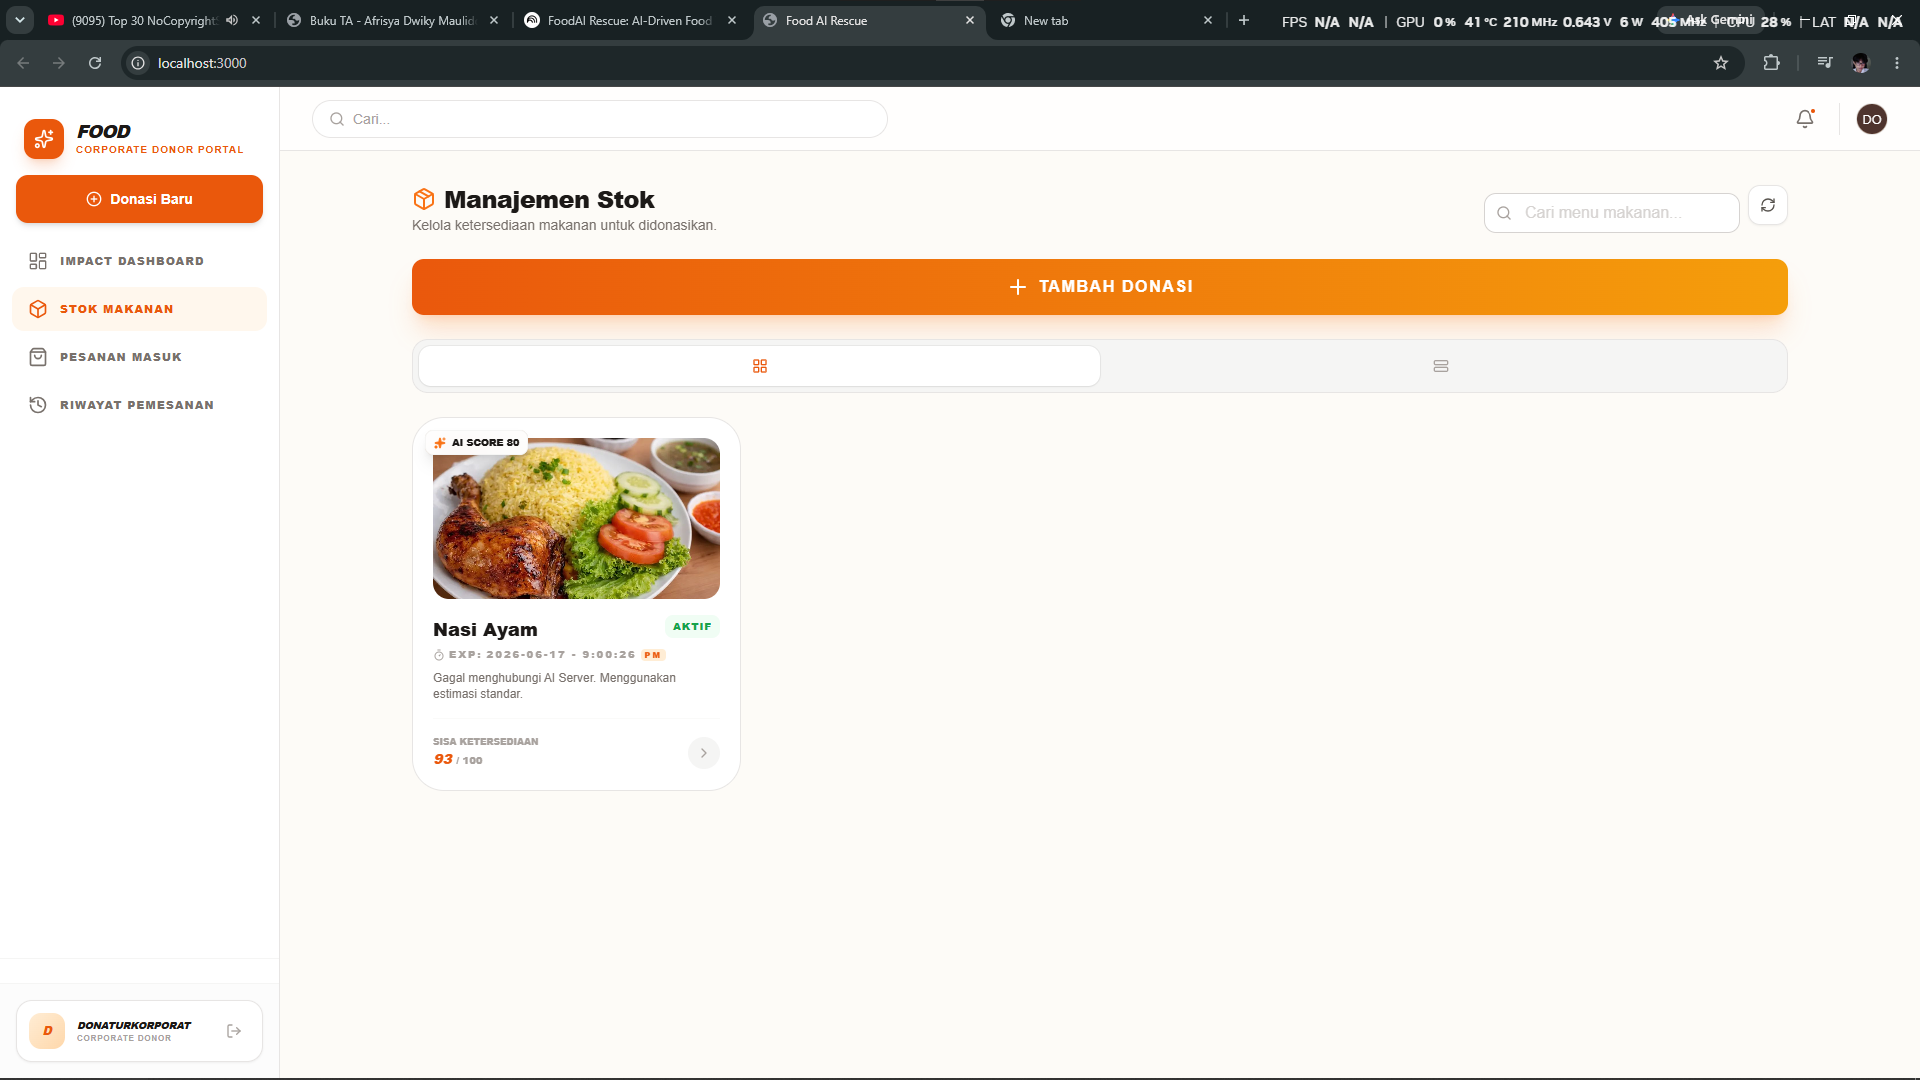
\includegraphics[width=\linewidth]{image/bab4/UserManual/InputDonasi/1-ManajemenStok.png}
    \caption{Manajemen Stok}
\end{figure}

\begin{figure}[H]
    \centering
    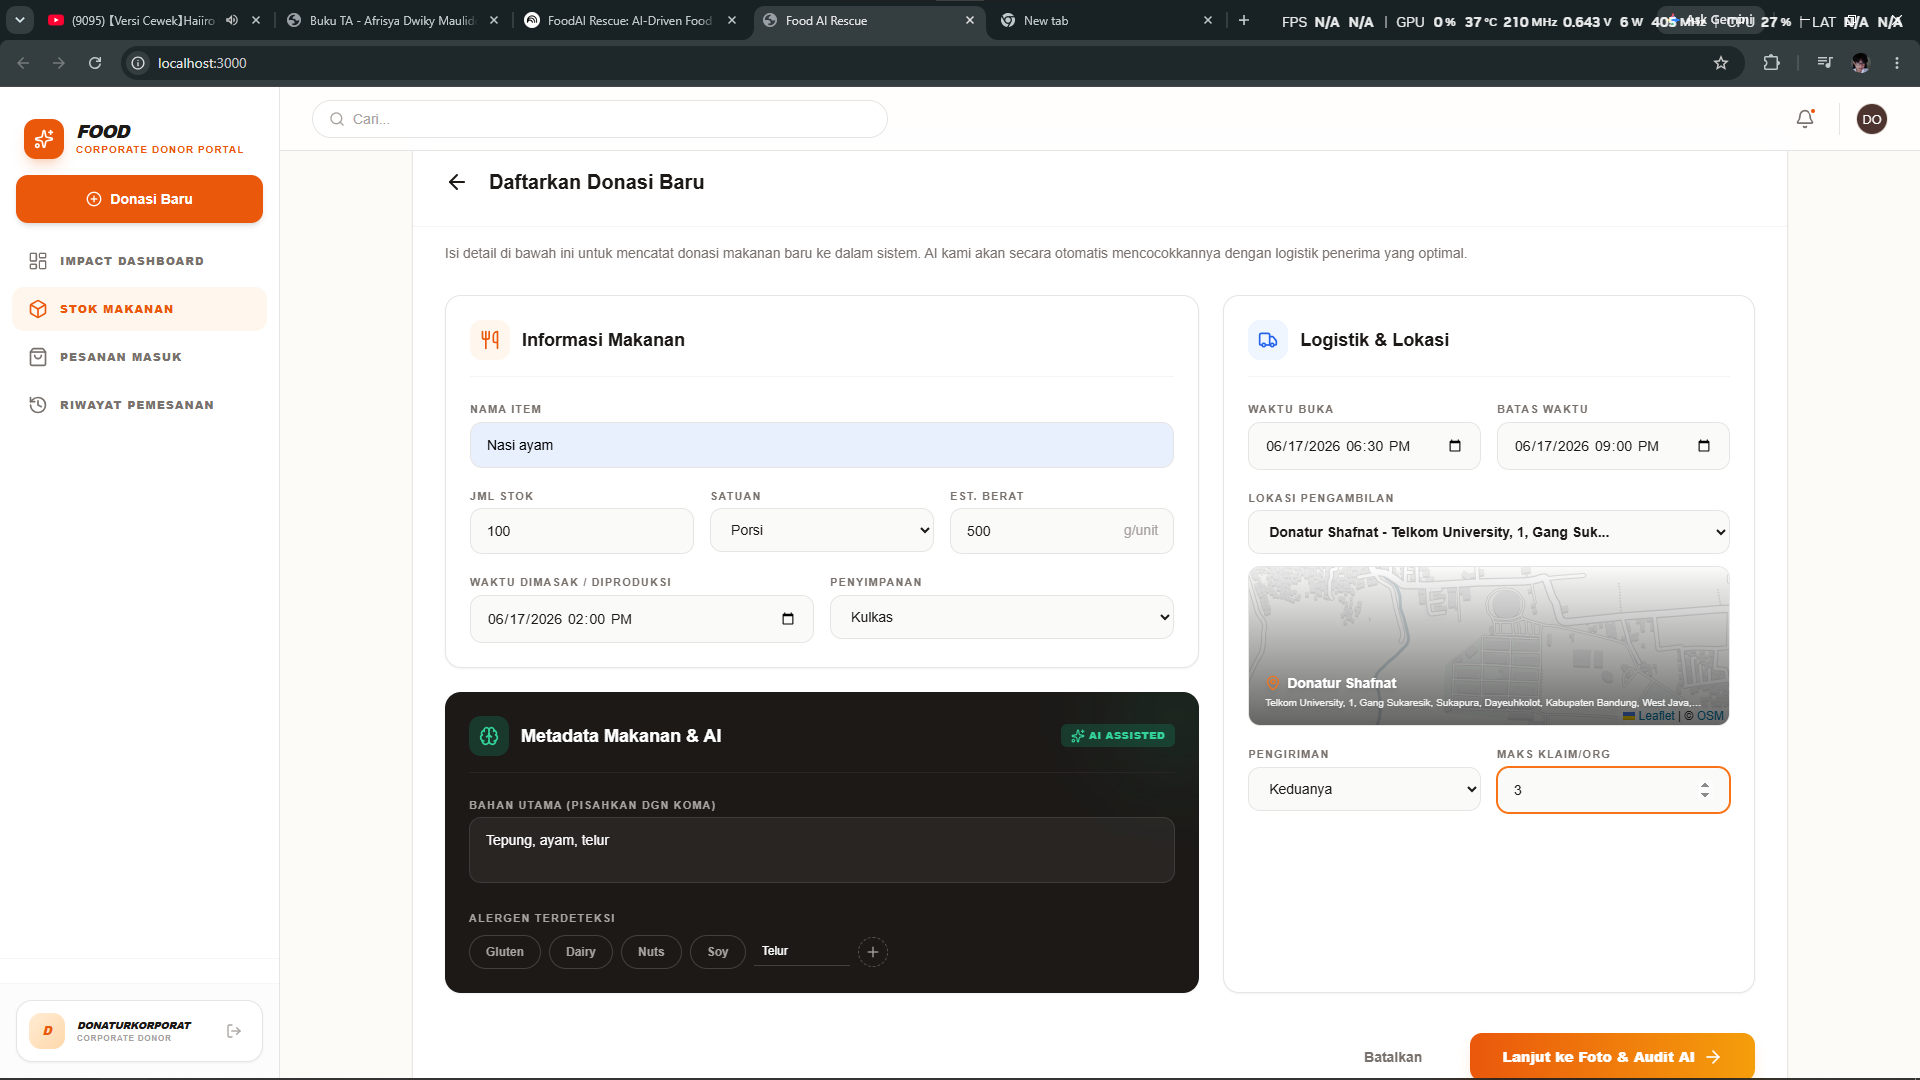
\includegraphics[width=\linewidth]{image/bab4/UserManual/InputDonasi/2-InputDataDonasi.png}
    \caption{Input Data Donasi}
\end{figure}

\begin{figure}[H]
    \centering
    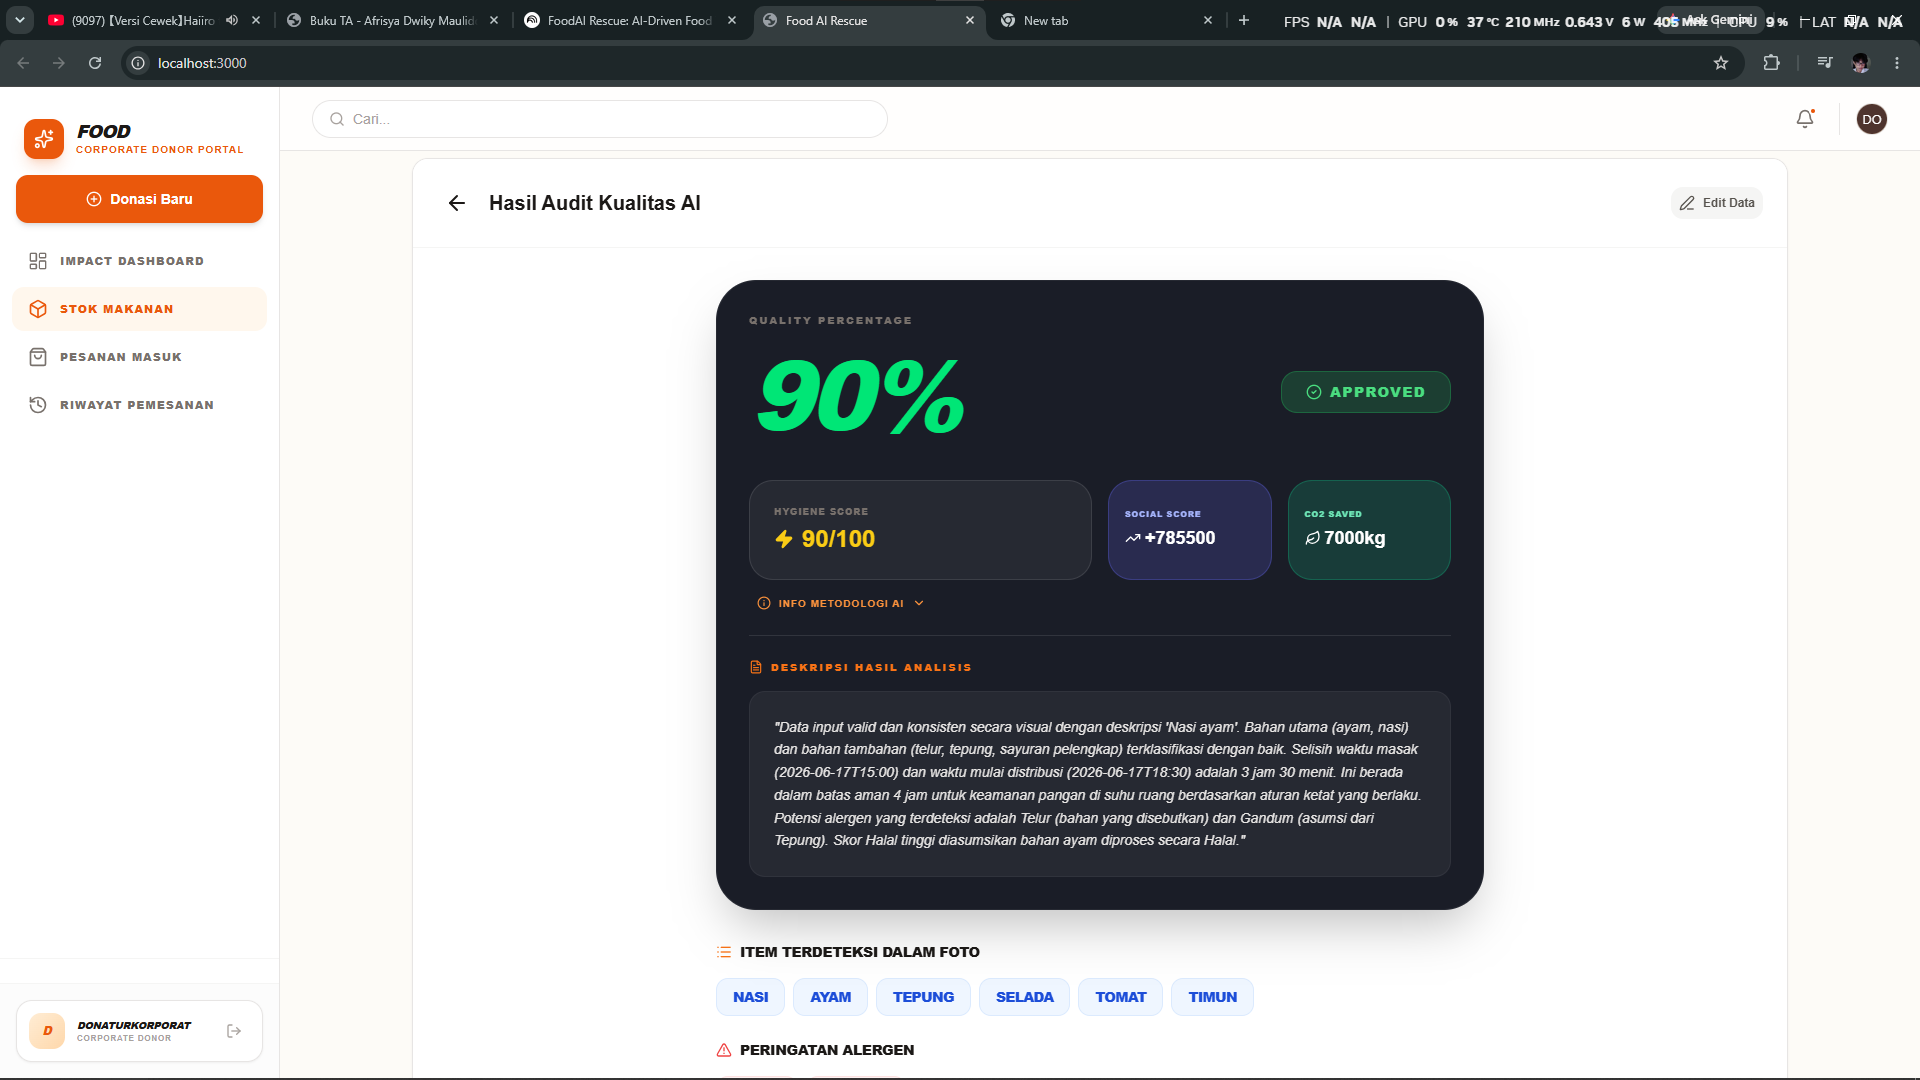
\includegraphics[width=\linewidth]{image/bab4/UserManual/InputDonasi/3-HasilAudit.png}
    \caption{Hasil Audit AI}
\end{figure}



\subsubsection{Proses Menerima dan Memproses Pesanan Masuk}
Langkah-langkah menerima pesanan dari penerima donasi:
\begin{enumerate}[label=\arabic*.]
    \item Buka menu \textbf{Pesanan Aktif} (Kelola Pesanan).
    \item Tekan pada pesanan yang masuk untuk melihat rincian (\textit{Detail Request}), lalu tekan setujui (\textit{Terima Request}).
\end{enumerate}

\begin{figure}[H]
    \centering
    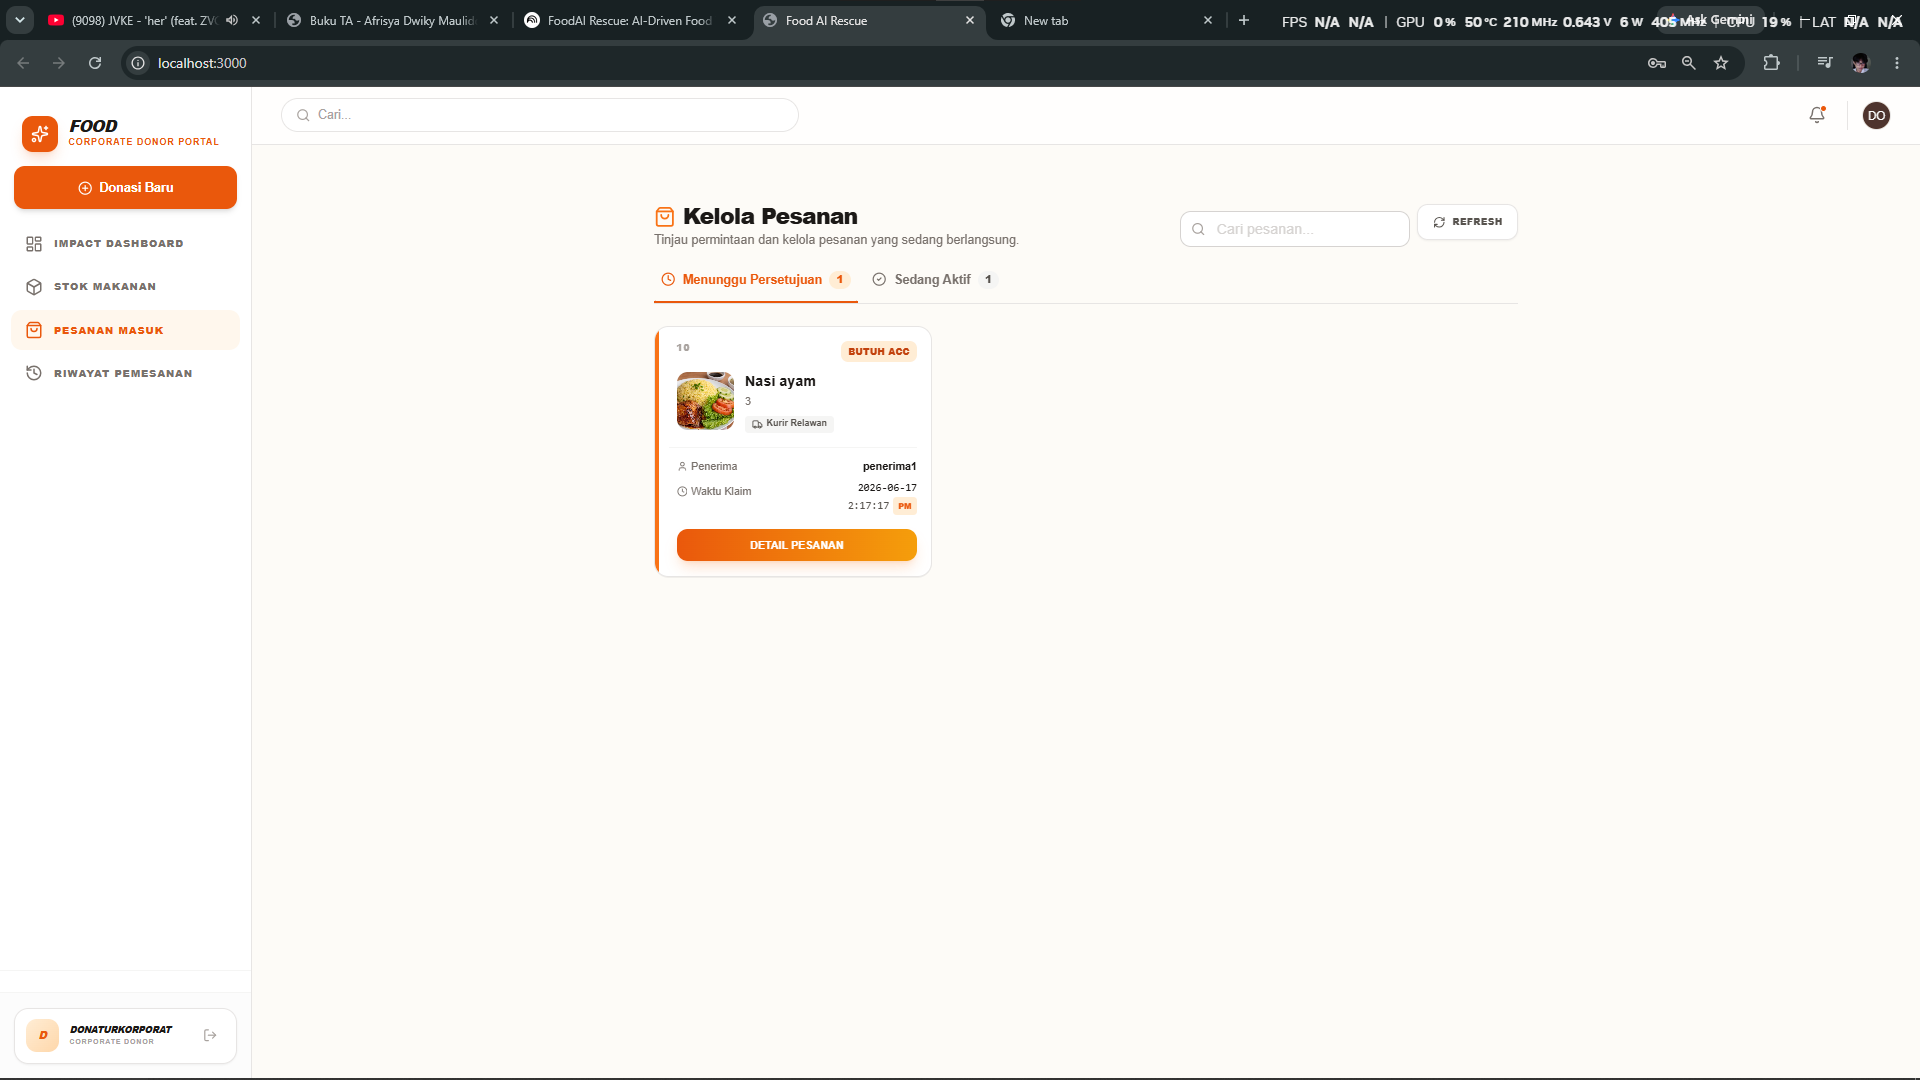
\includegraphics[width=\linewidth]{image/bab4/UserManual/TerimaPesanan/1-KelolaPesanan.png}
    \caption{Menu Pesanan Aktif}
\end{figure}

\begin{figure}[H]
    \centering
    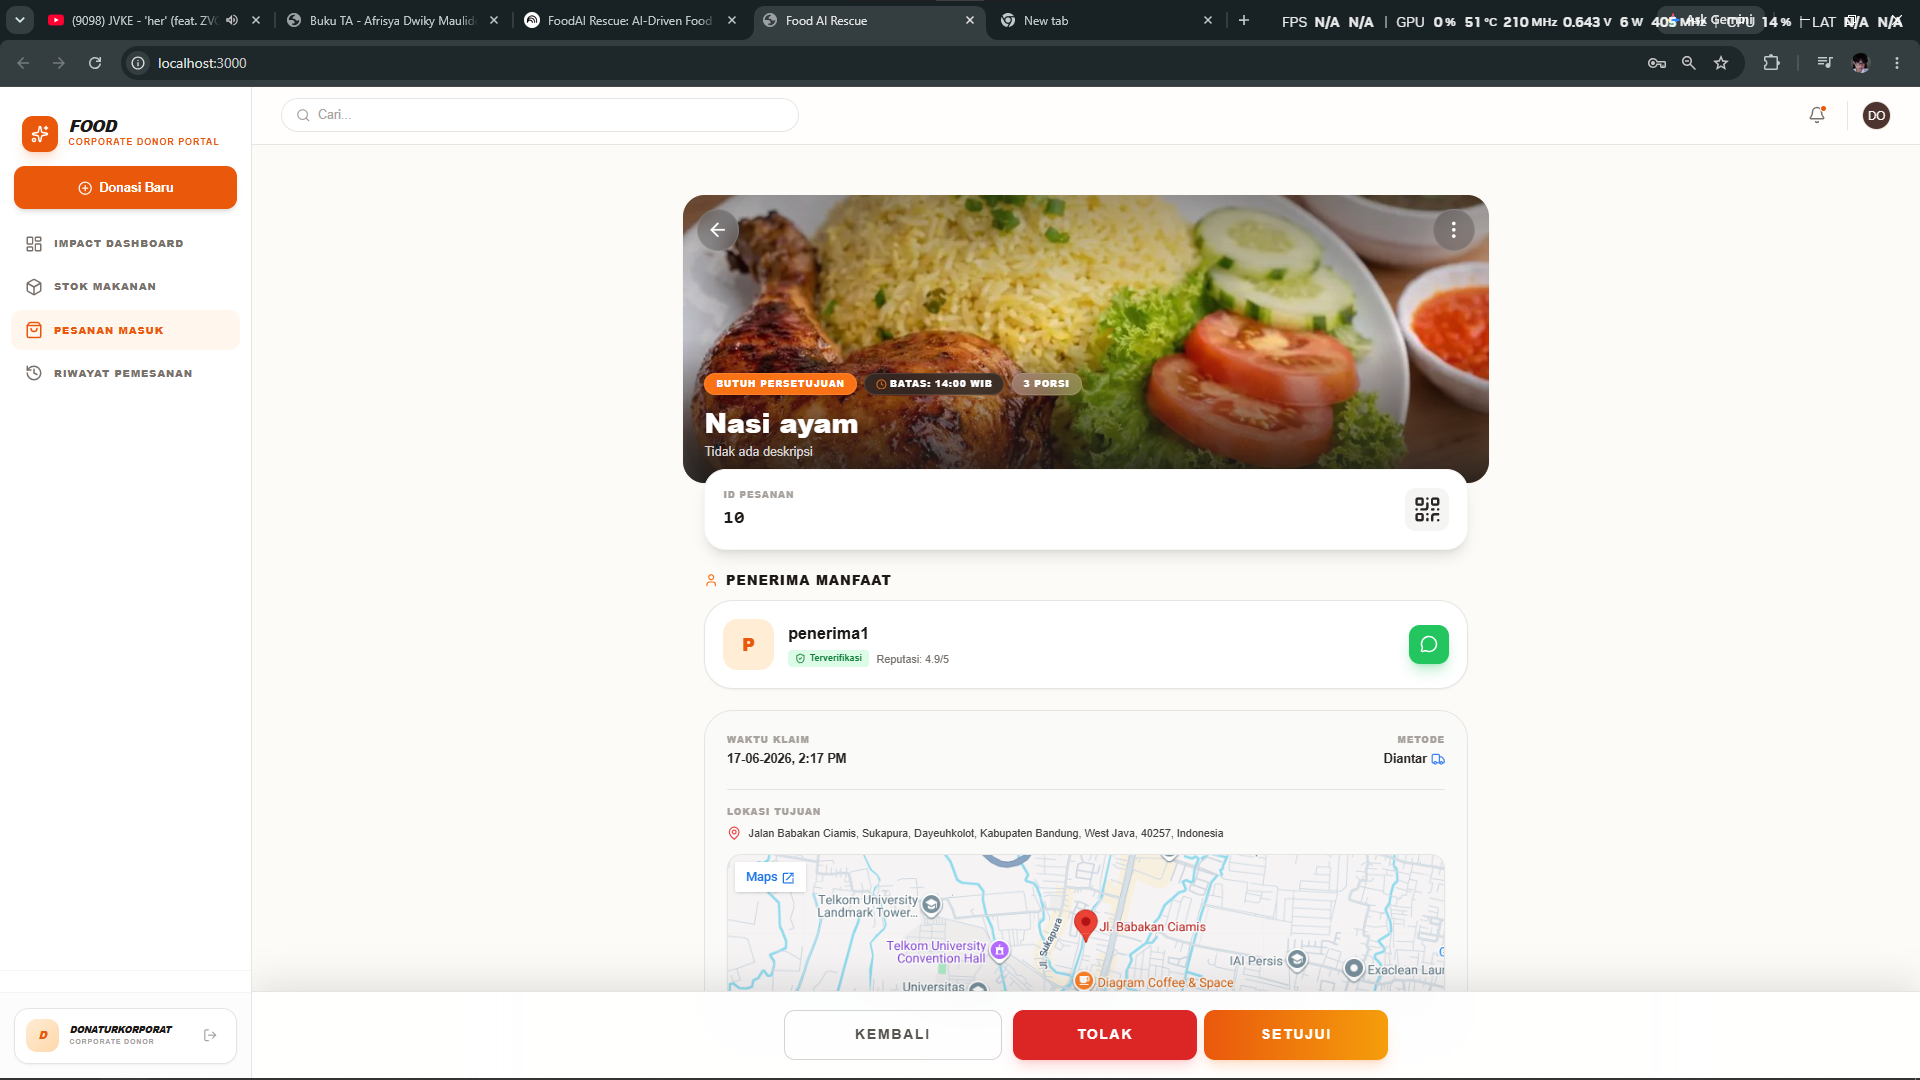
\includegraphics[width=\linewidth]{image/bab4/UserManual/TerimaPesanan/2-DetailRequest.png}
    \caption{Detail Permintaan (\textit{Request})}
\end{figure}



\subsubsection{Proses Verifikasi Penyerahan Donasi ke Kurir}
Langkah-langkah untuk mengonfirmasi serah terima logistik dengan relawan:
\begin{enumerate}[label=\arabic*.]
    \item Buka menu \textbf{Pesanan Aktif} dan pilih pesanan dengan status \textit{Siap Diambil}.
    \item Buka Detail Pesanan, dan pilih opsi pindai Kode QR atau masukkan resi pengantaran manual milik relawan kurir untuk menyerahkan donasi secara nirkontak.
\end{enumerate}

\begin{figure}[H]
    \centering
    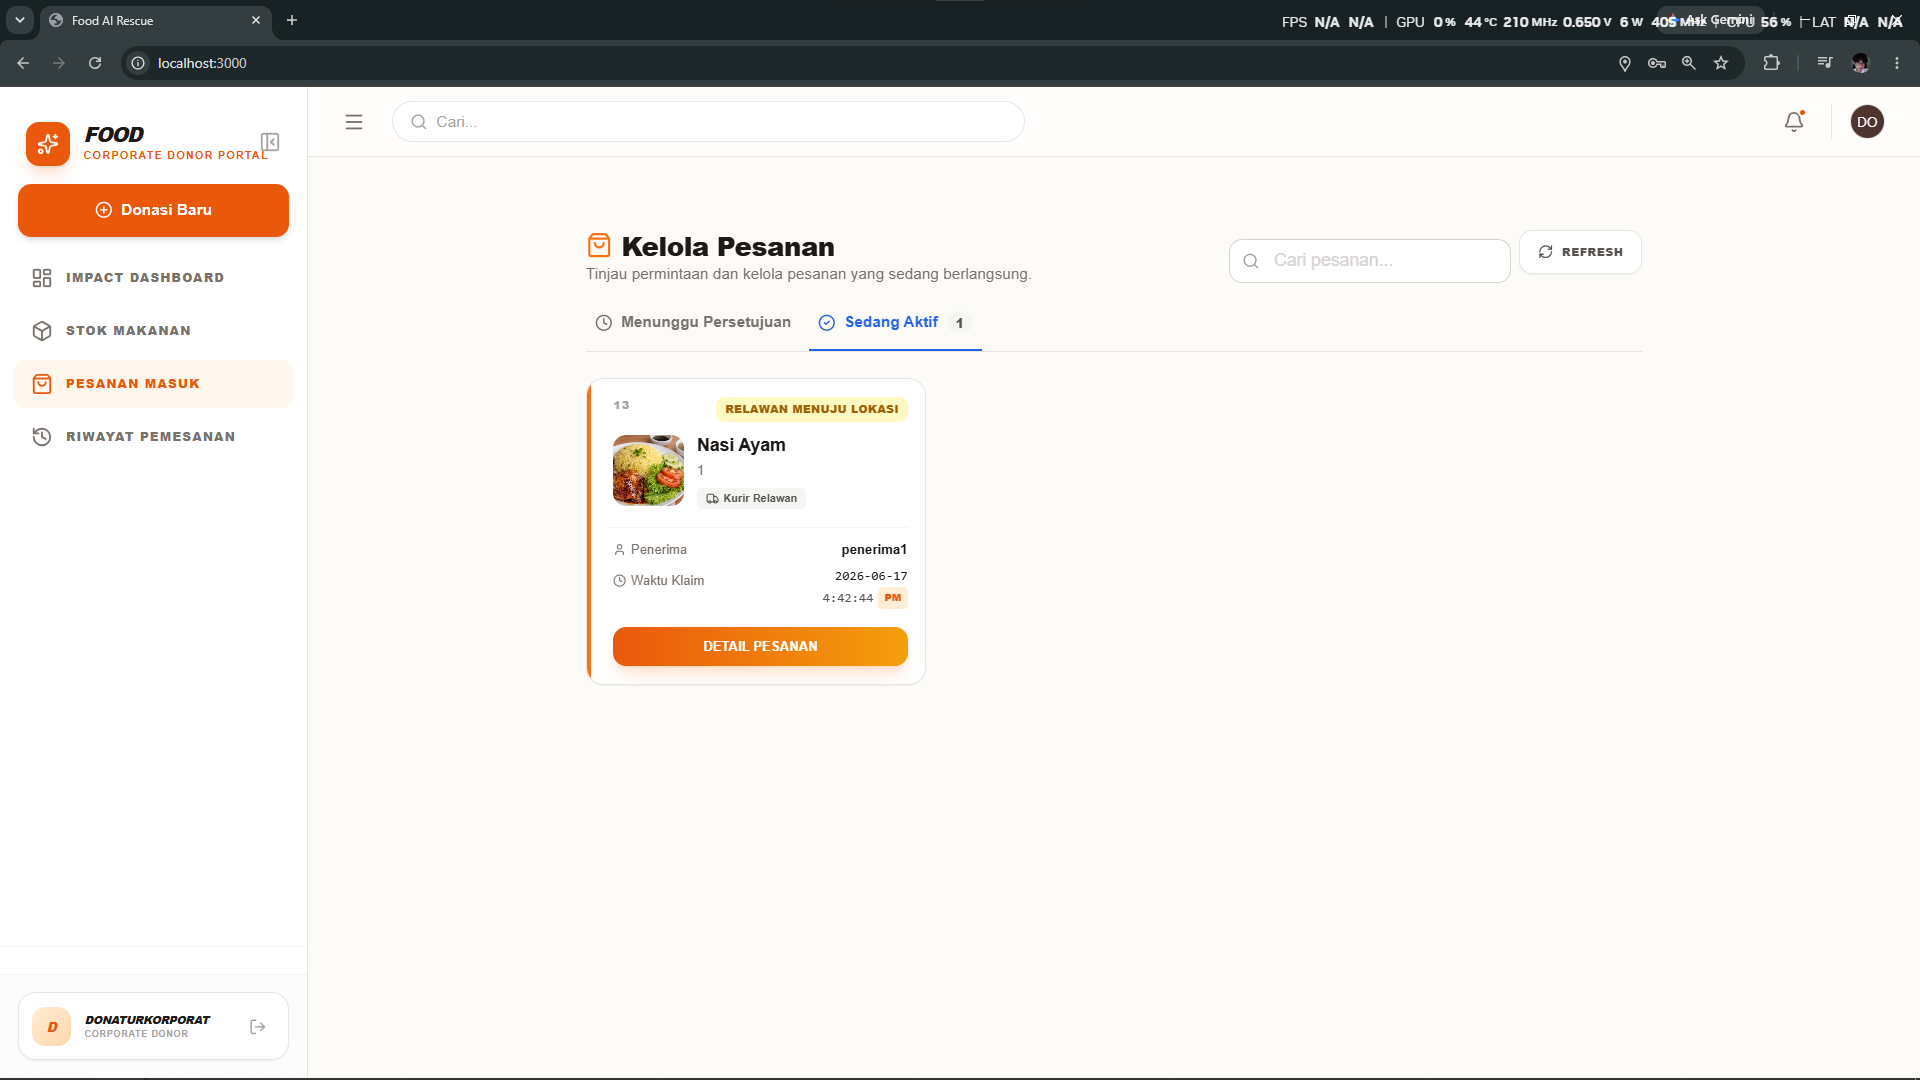
\includegraphics[width=\linewidth]{image/bab4/UserManual/VerifikasiRelawan/1-KelolaPesanan.png}
    \caption{Daftar Pesanan Aktif}
\end{figure}

\begin{figure}[H]
    \centering
    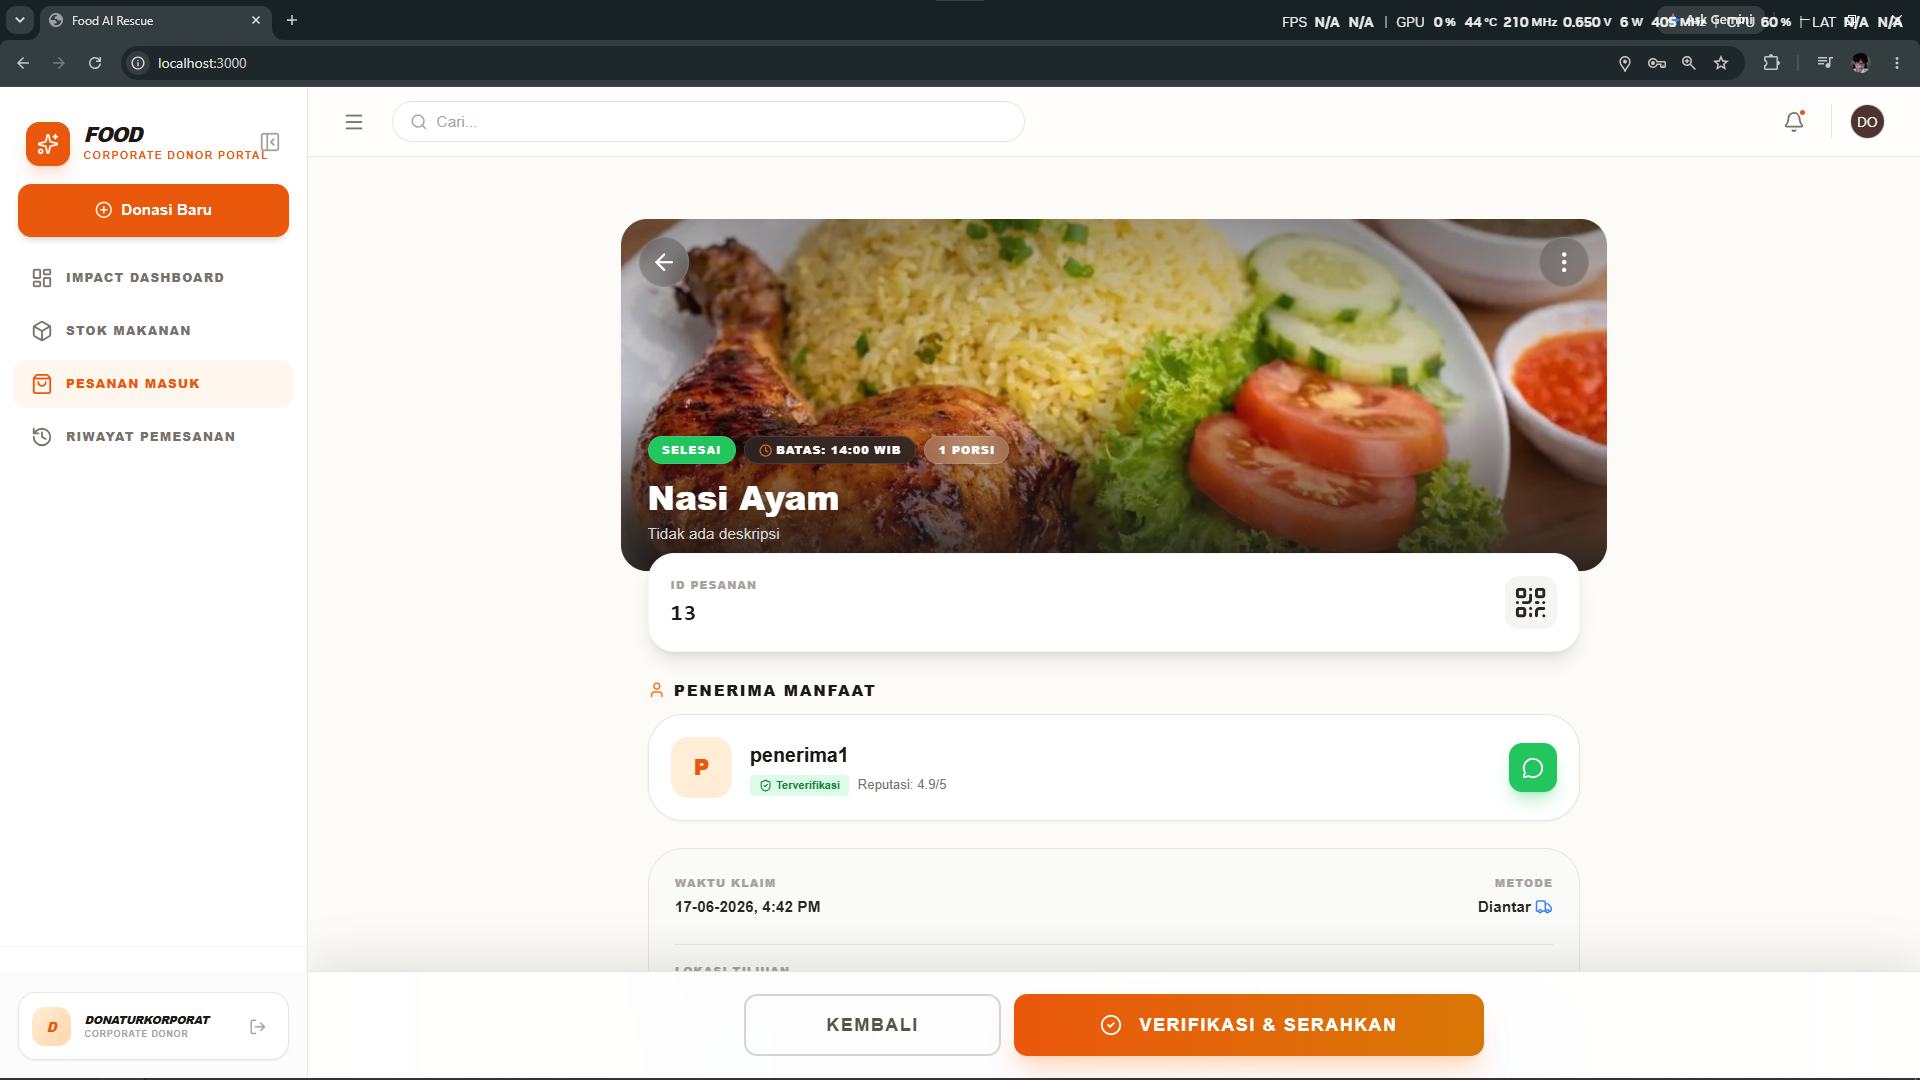
\includegraphics[width=\linewidth]{image/bab4/UserManual/VerifikasiRelawan/2-DetailPesanan.png}
    \caption{Detail Pesanan}
\end{figure}



\begin{figure}[H]
    \centering
    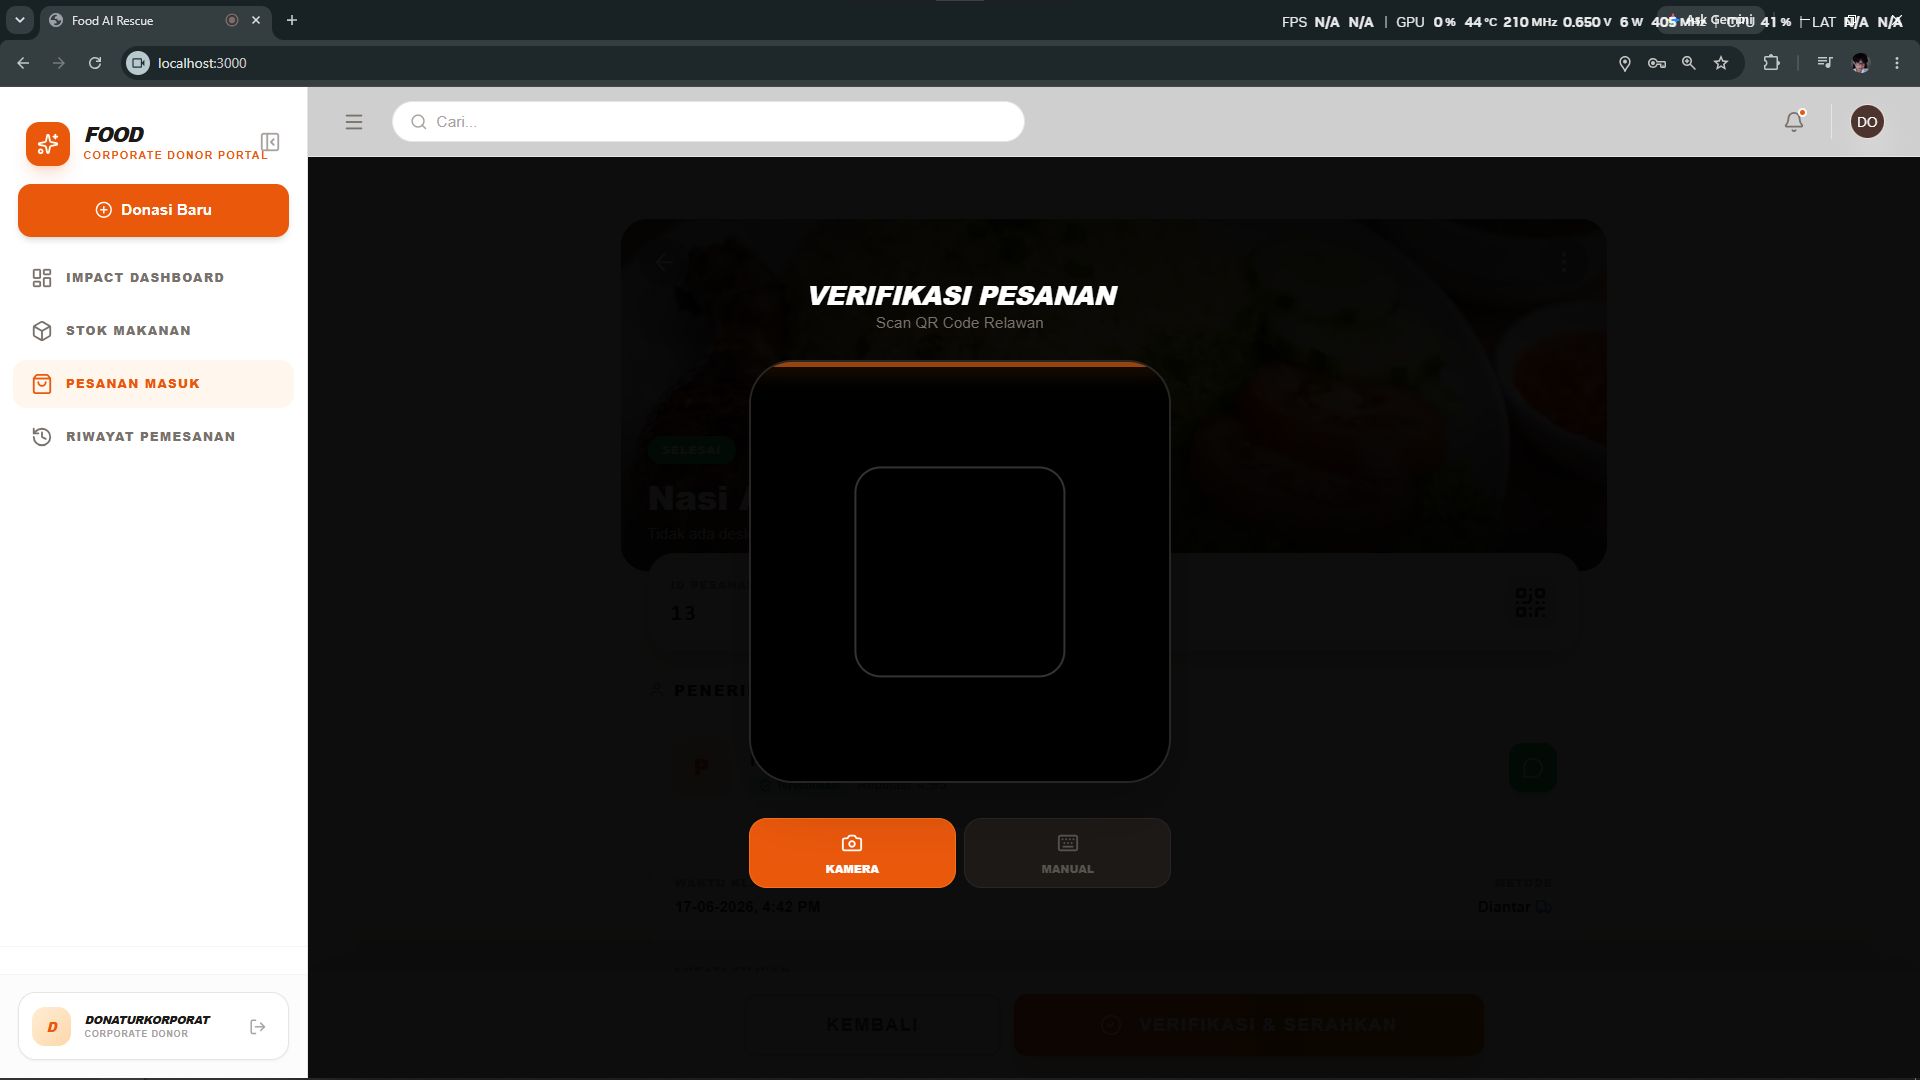
\includegraphics[width=\linewidth]{image/bab4/UserManual/VerifikasiRelawan/3-ScanQR.png}
    \caption{\textit{Scan}}
\end{figure}

\begin{figure}[H]
    \centering
    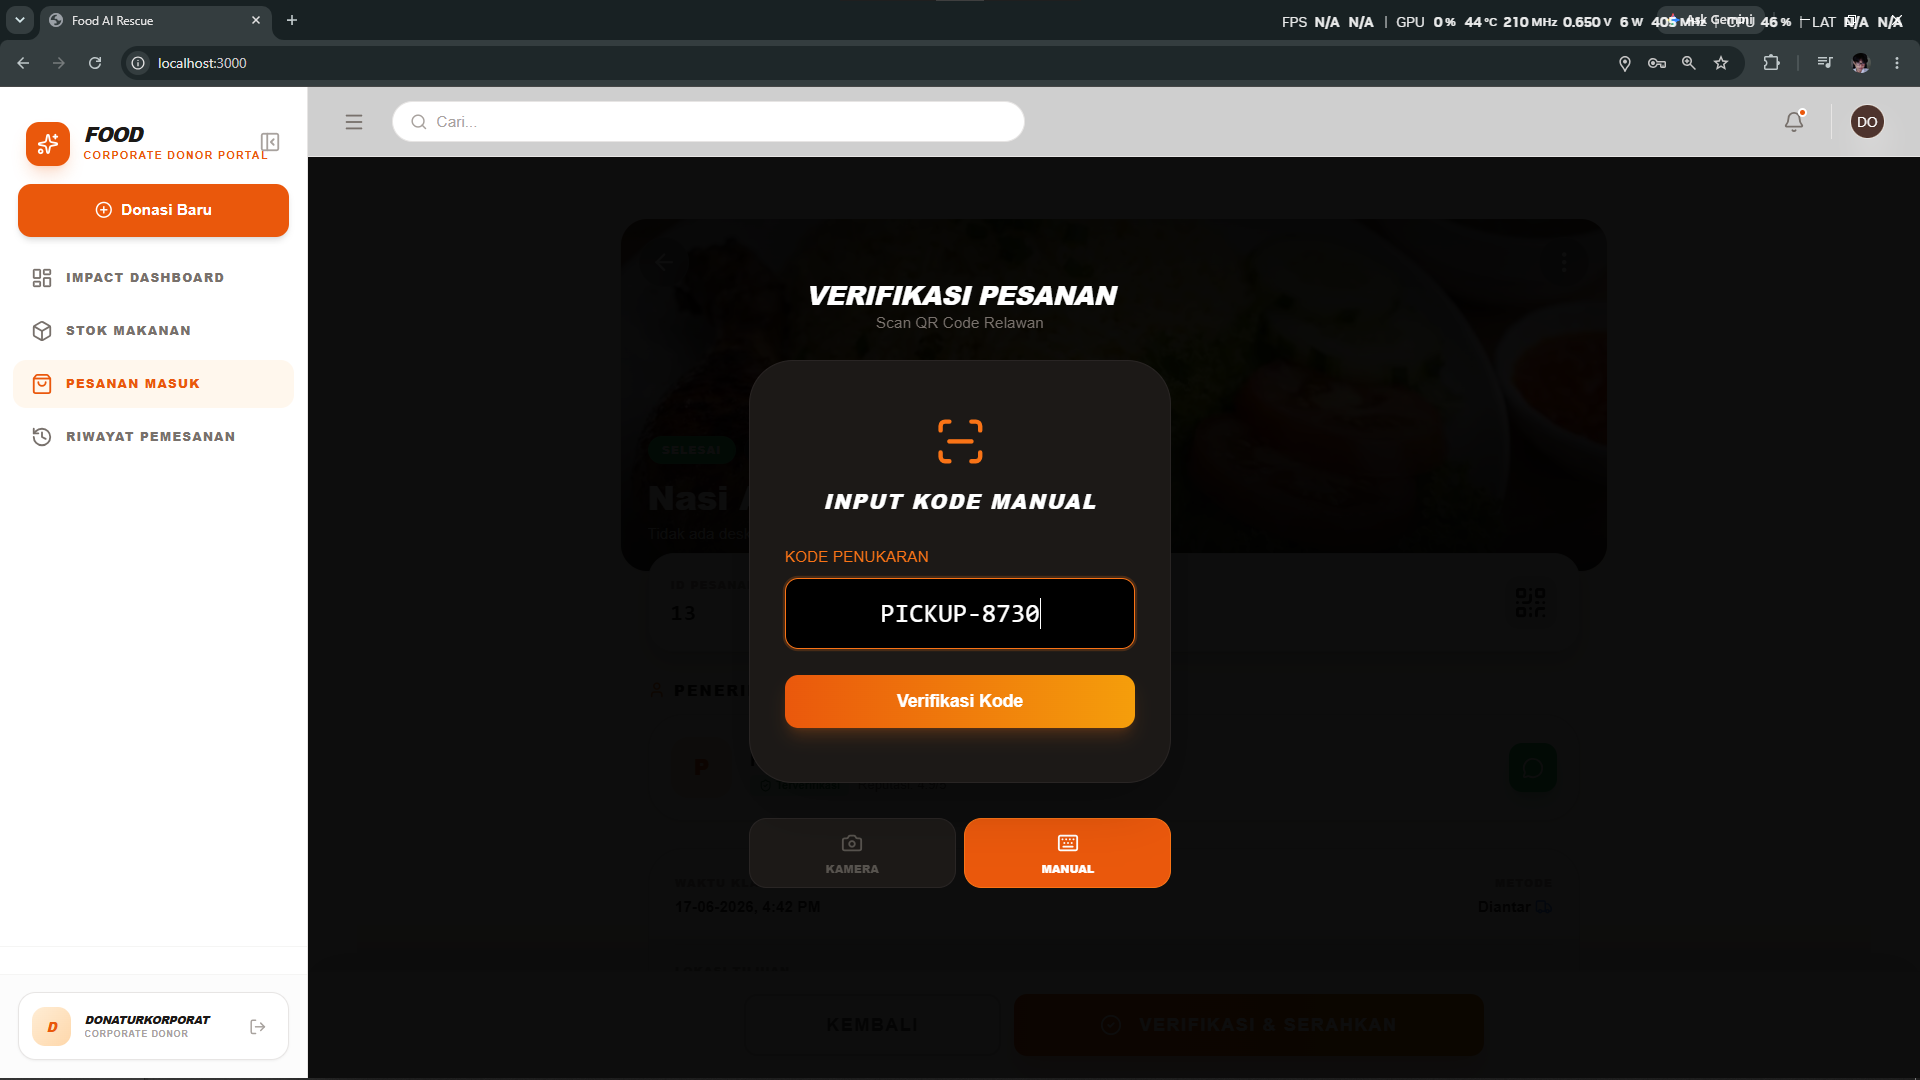
\includegraphics[width=\linewidth]{image/bab4/UserManual/VerifikasiRelawan/4-InputManualCode.png}
    \caption{Input Kode Manual}
\end{figure}



\textbf{C. Pengguna Penerima (Panti Asuhan / Individu)}

\subsubsection{Proses Klaim Donasi Makanan}
Langkah-langkah untuk melakukan pemesanan (klaim) surplus makanan:
\begin{enumerate}[label=\arabic*.]
    \item Buka dasbor radar penerima (\textit{Home Radar}) untuk menelusuri ketersediaan donasi terdekat.
    \item Tekan pada makanan yang diinginkan untuk membaca detail kandungan gizi dan jarak.
    \item Tekan tombol \textbf{Klaim Sekarang} dan pilih metode pengiriman, kemudian konfirmasi pesanan tersebut.
    \item Sistem akan menampilkan layar pemberitahuan bahwa klaim telah terkirim.
\end{enumerate}

\begin{figure}[H]
    \centering
    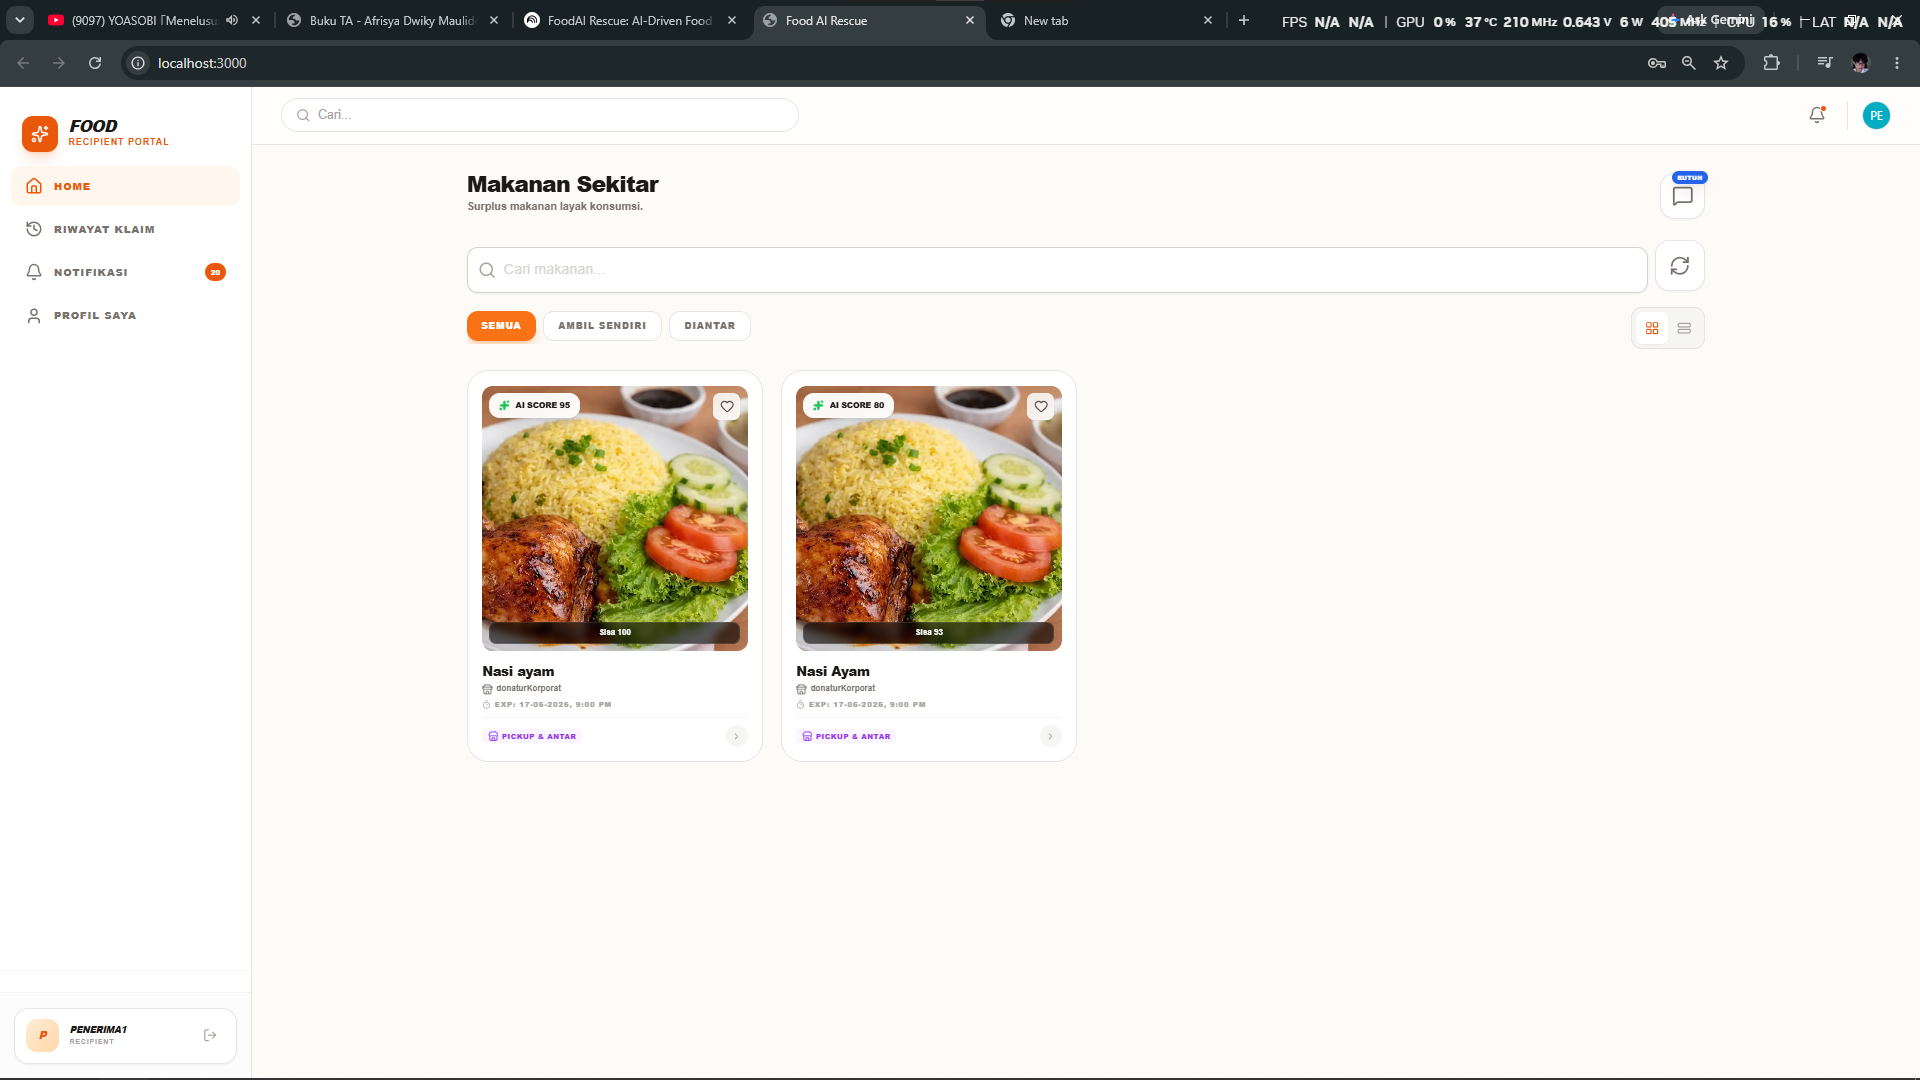
\includegraphics[width=\linewidth]{image/bab4/UserManual/KlaimDonasi/1-HomeRadar.png}
    \caption{Radar Makanan Terdekat}
\end{figure}

\begin{figure}[H]
    \centering
    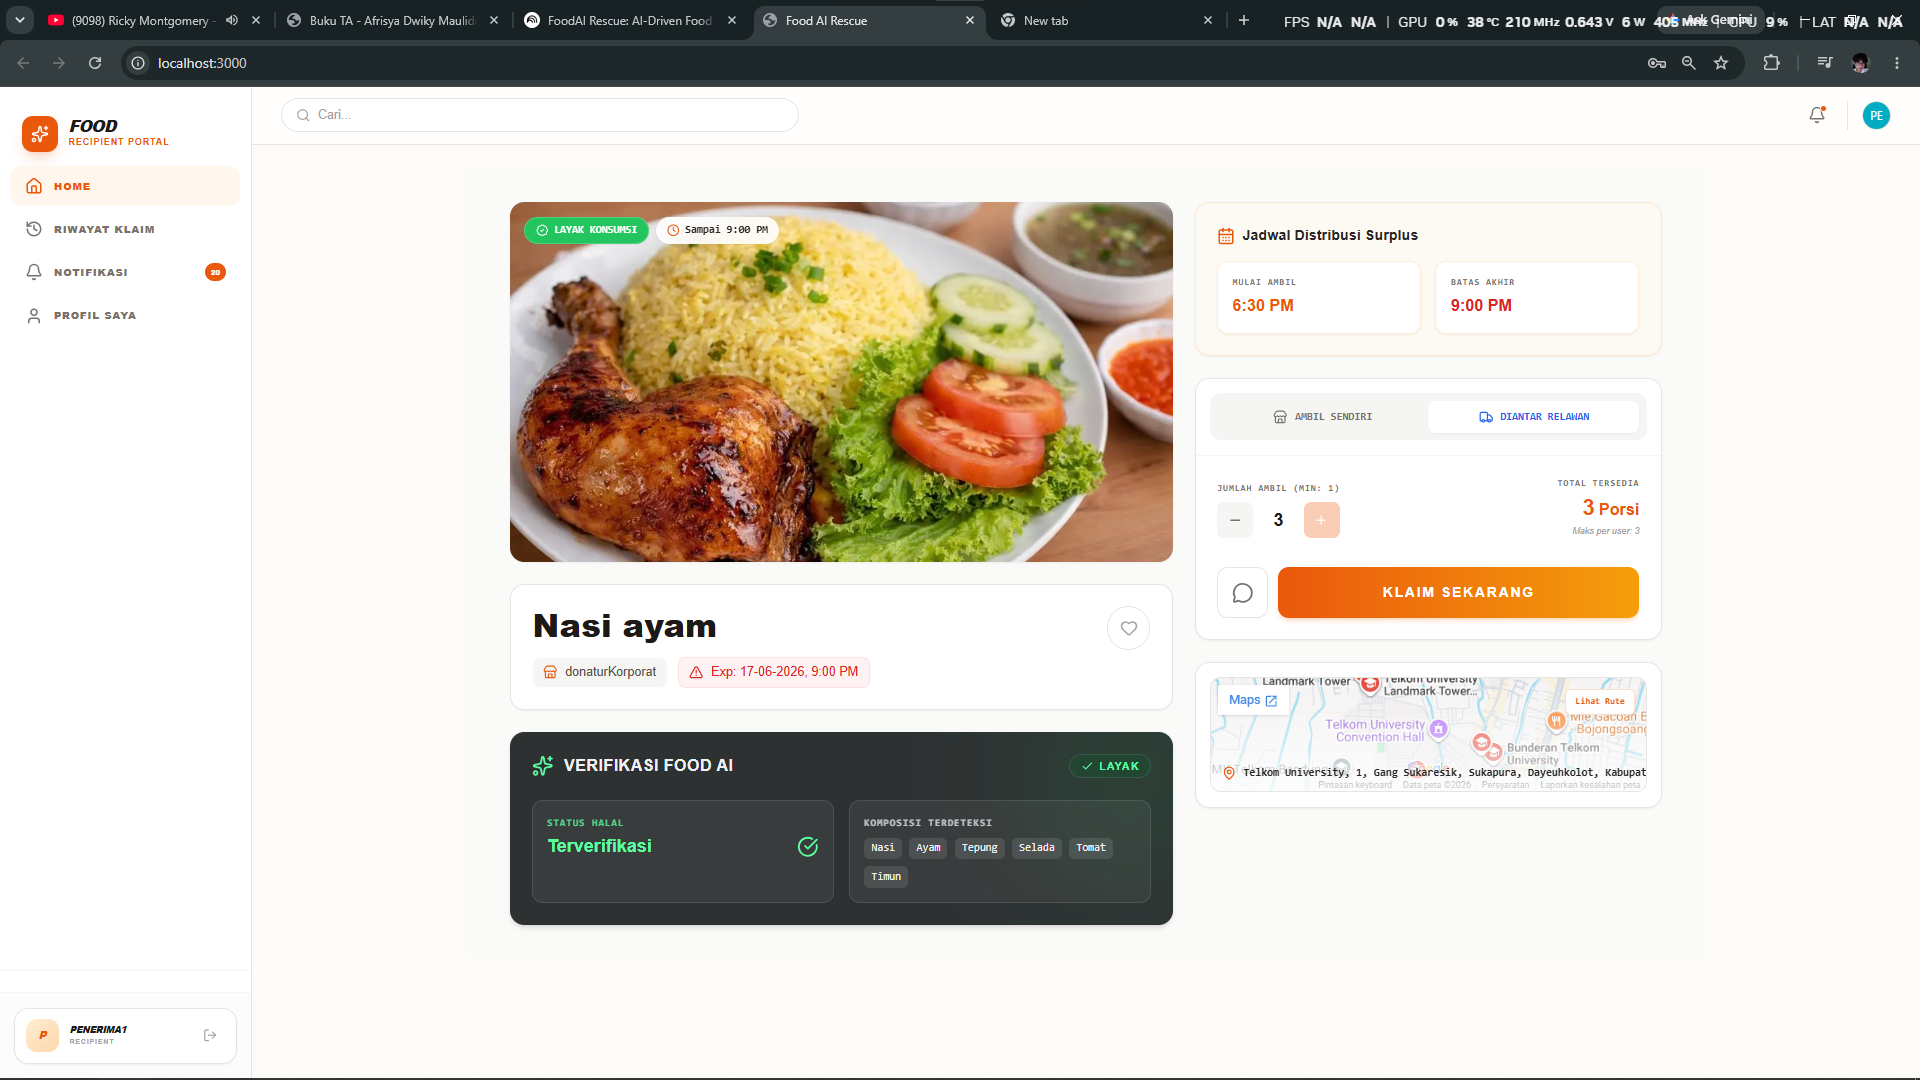
\includegraphics[width=\linewidth]{image/bab4/UserManual/KlaimDonasi/2-DetailMakanan.png}
    \caption{Detail Makanan}
\end{figure}



\begin{figure}[H]
    \centering
    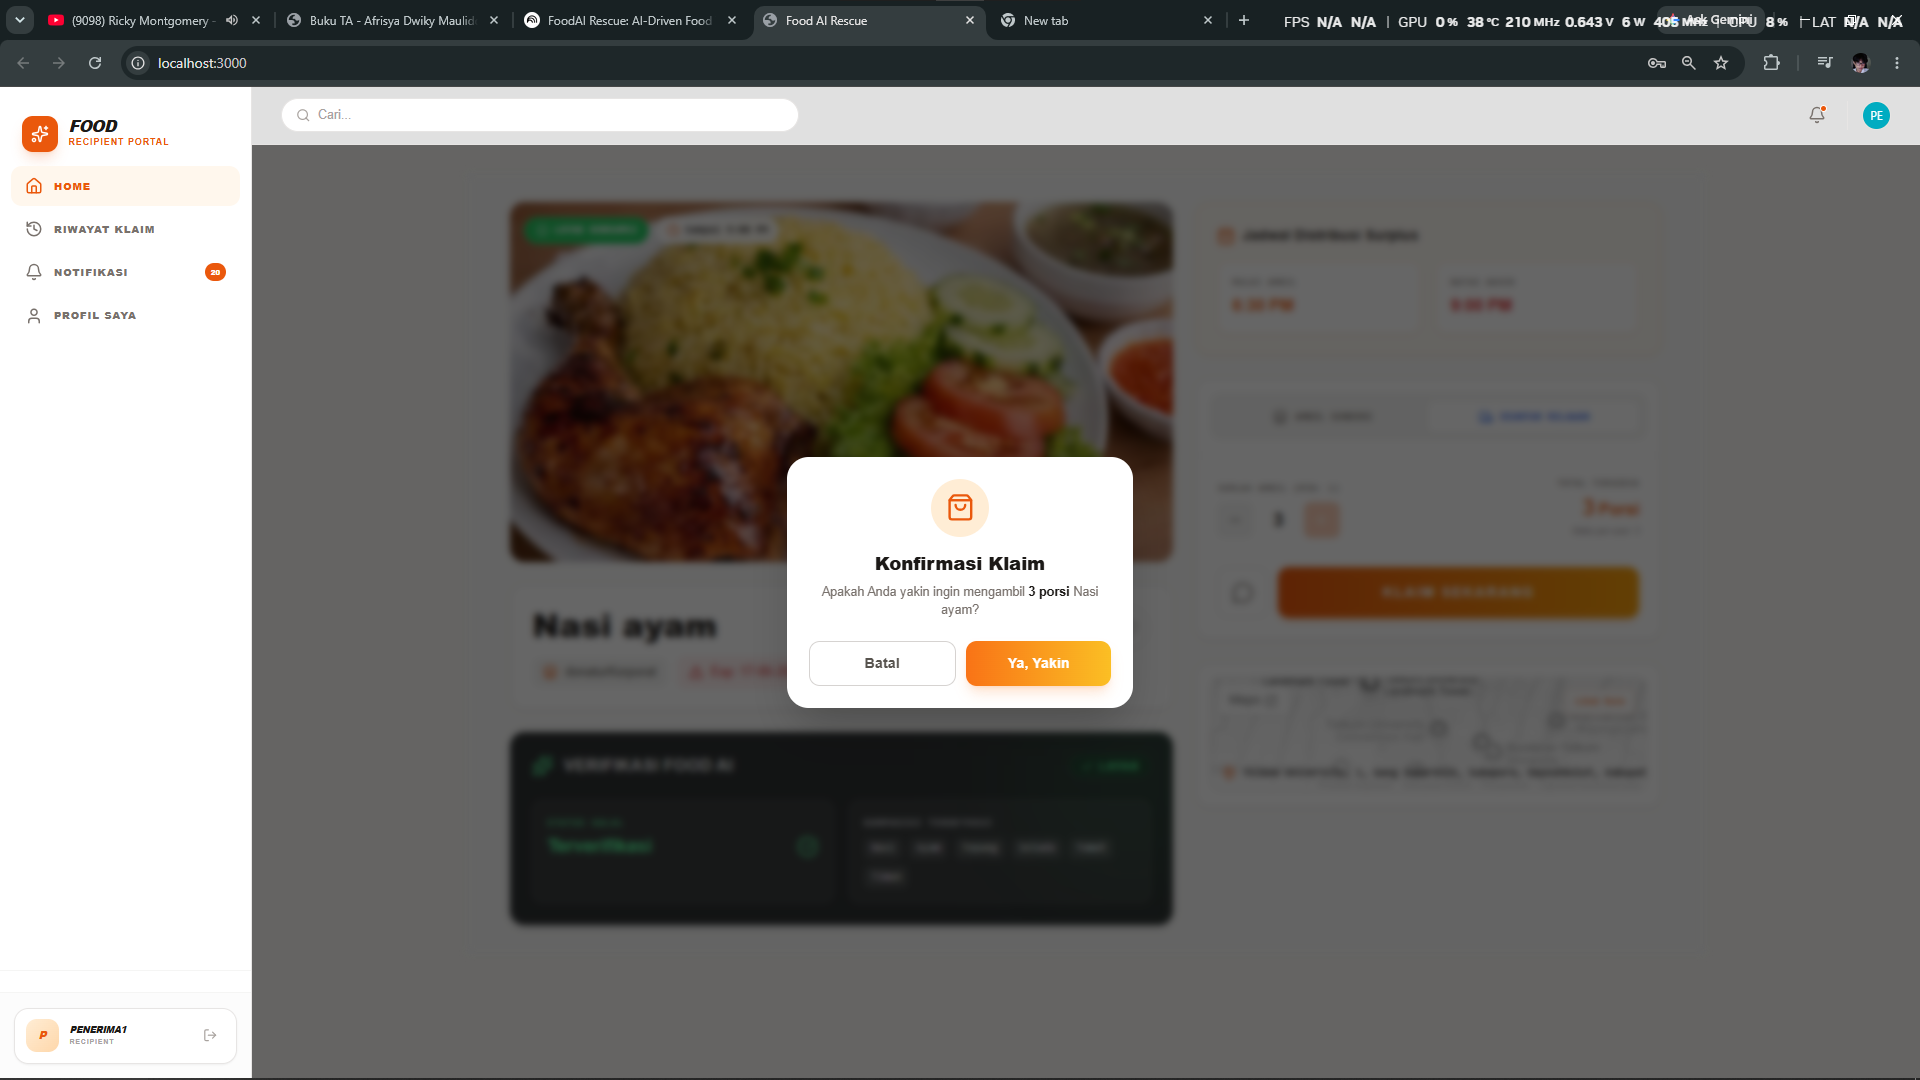
\includegraphics[width=\linewidth]{image/bab4/UserManual/KlaimDonasi/3-KonfirmasiKlaim.png}
    \caption{Konfirmasi Klaim}
\end{figure}

\begin{figure}[H]
    \centering
    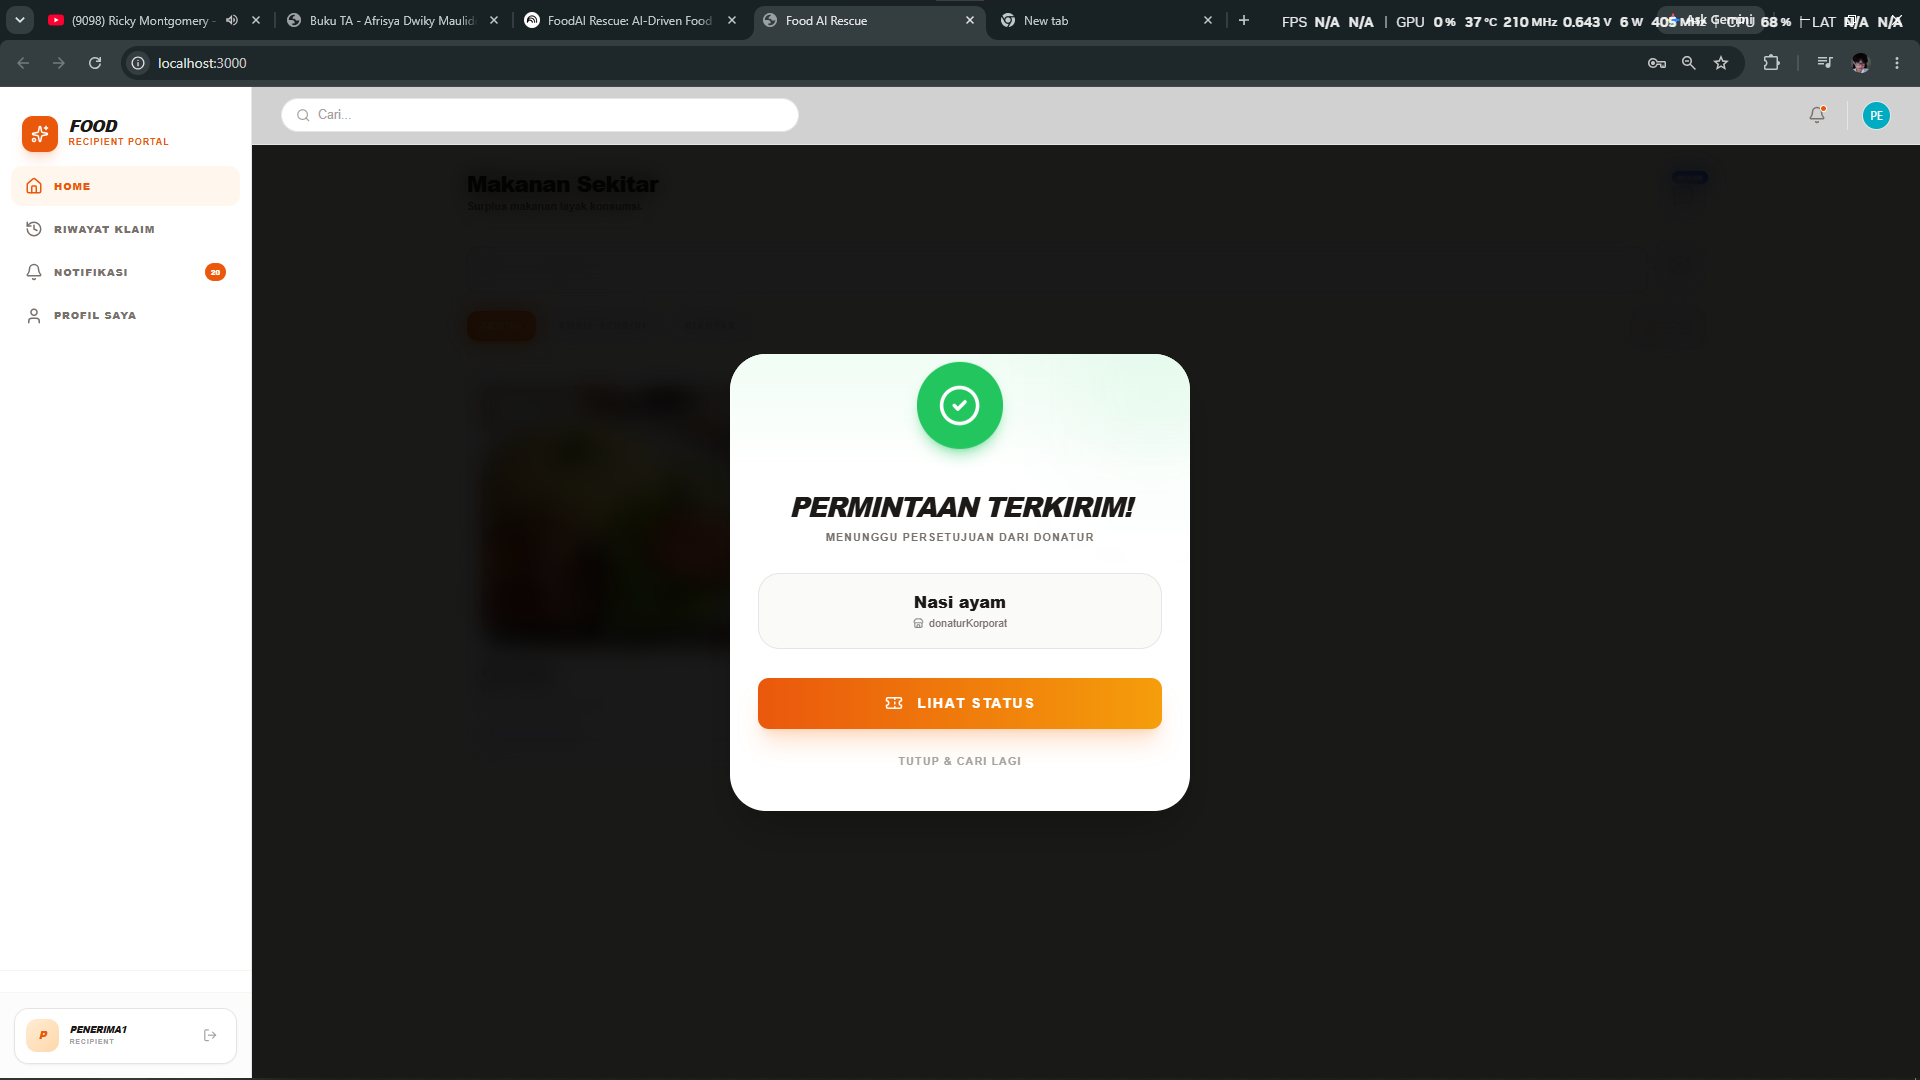
\includegraphics[width=\linewidth]{image/bab4/UserManual/KlaimDonasi/4-KlaimTerkirim.png}
    \caption{Notifikasi Klaim Terkirim}
\end{figure}



\textbf{D. Pengguna Relawan (Kurir Logistik)}

\subsubsection{Proses Mengambil Misi Penjemputan}
Langkah-langkah mengambil misi pengantaran dari katalog tugas:
\begin{enumerate}[label=\arabic*.]
    \item Buka daftar misi antrean pada dasbor \textit{Missions Board}.
    \item Tekan pada salah satu misi untuk melihat manifes rute penjemputan, lalu tekan \textbf{Ambil Misi Ini}.
\end{enumerate}

\begin{figure}[H]
    \centering
    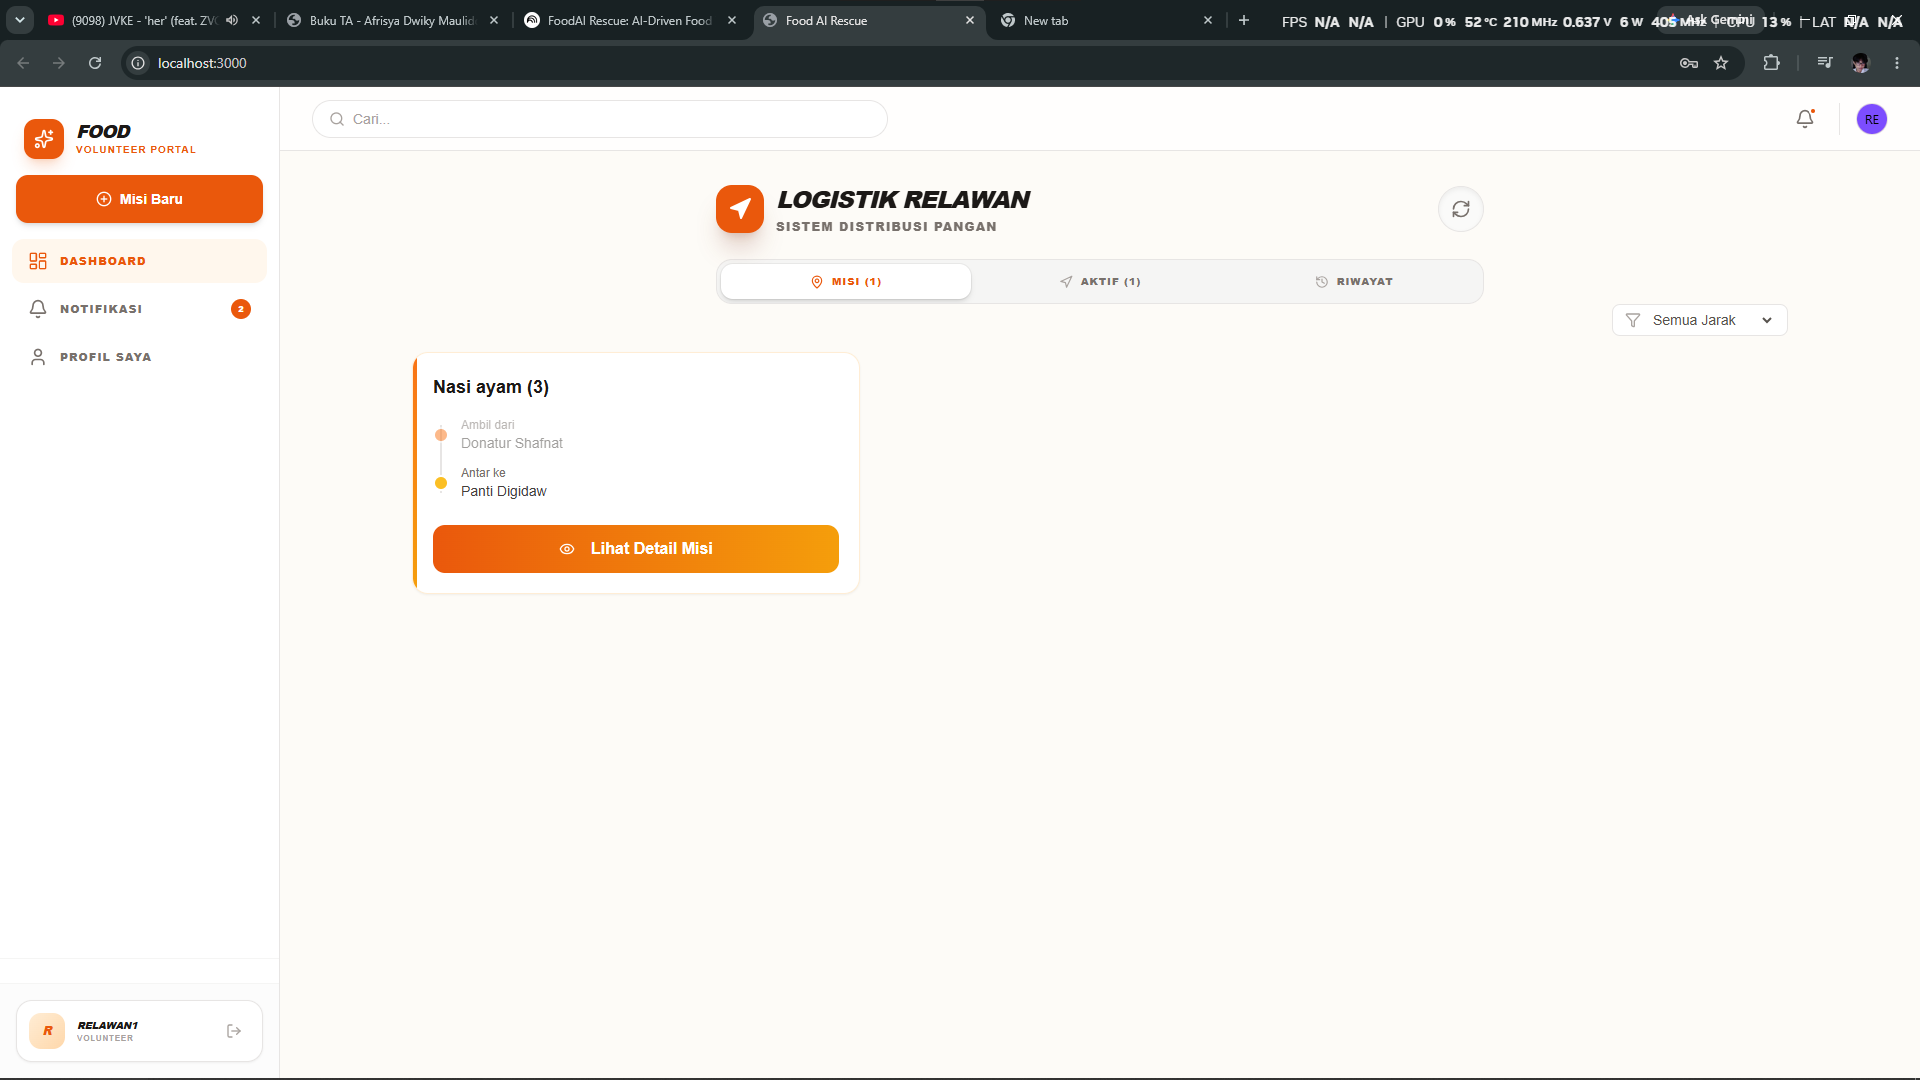
\includegraphics[width=\linewidth]{image/bab4/UserManual/AmbilMisi/1-MissionsBoard.png}
    \caption{Daftar Misi Antrean}
\end{figure}

\begin{figure}[H]
    \centering
    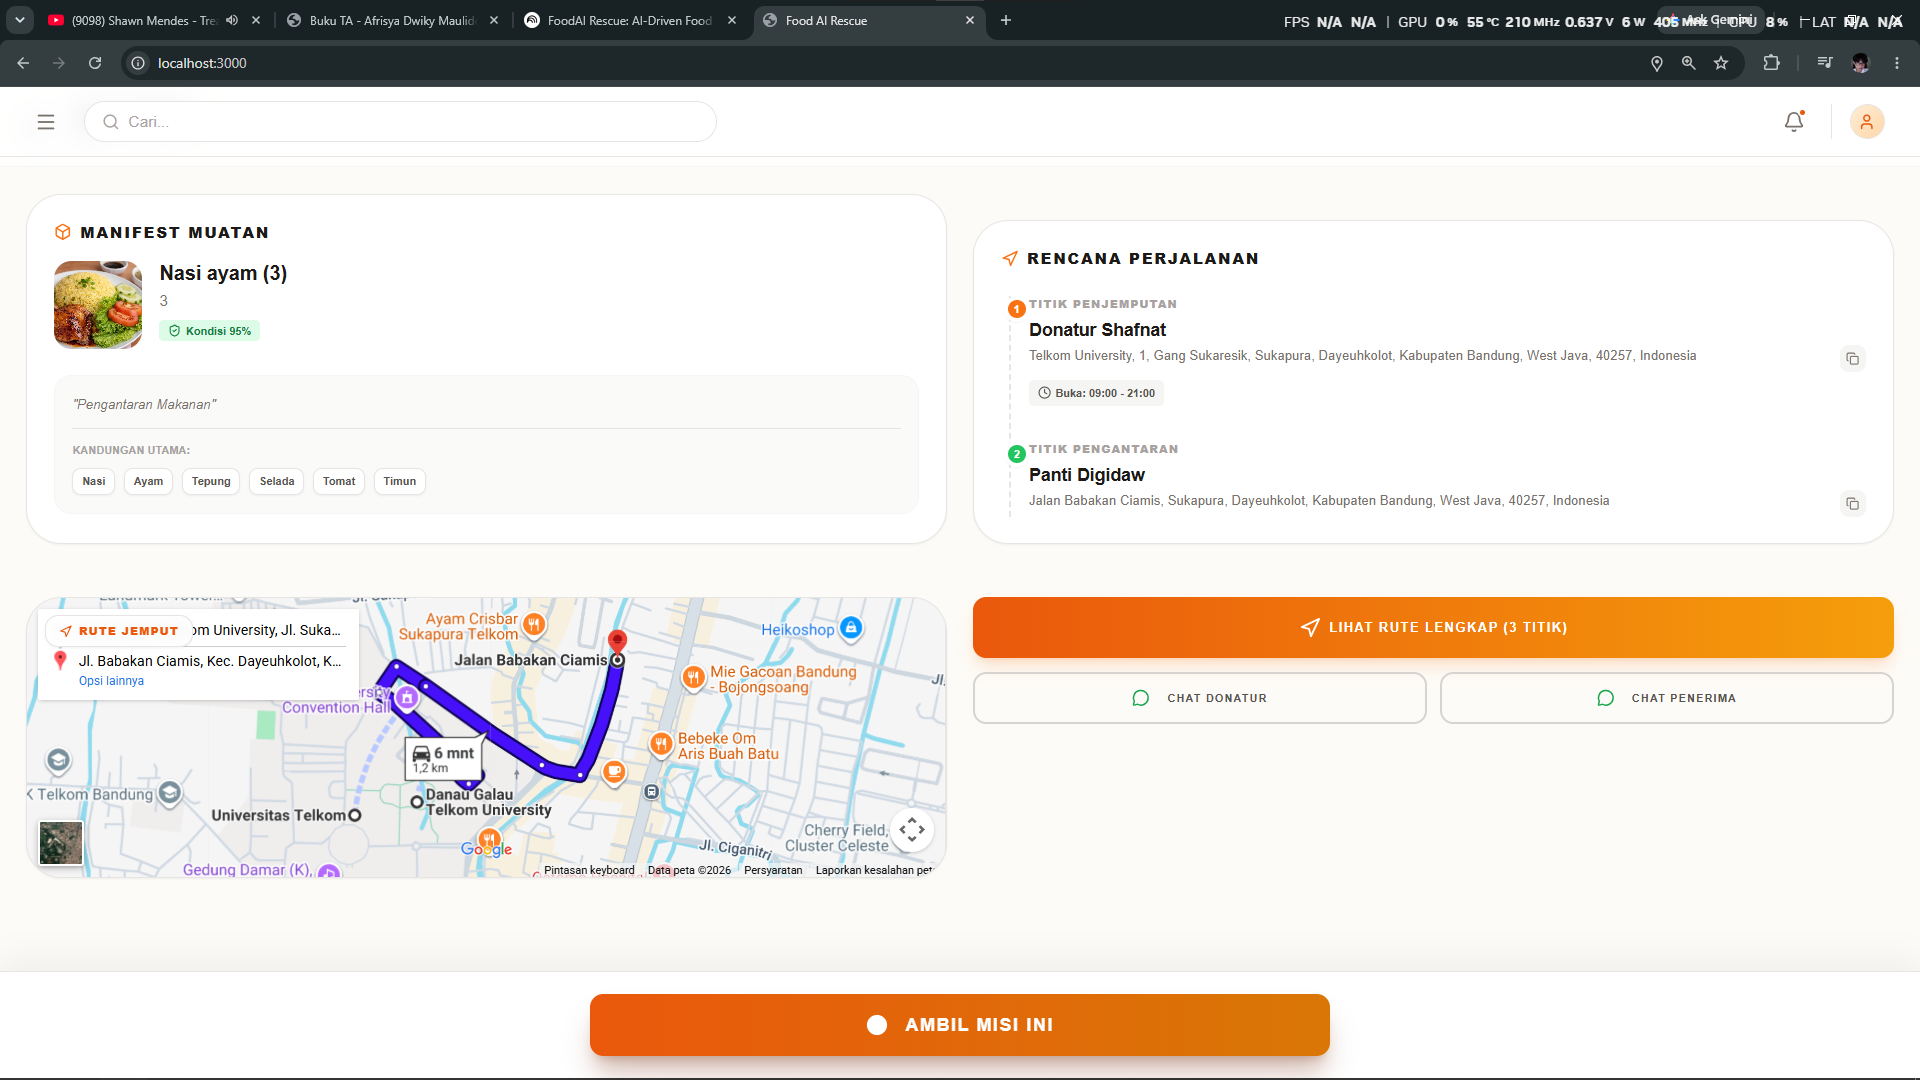
\includegraphics[width=\linewidth]{image/bab4/UserManual/AmbilMisi/2-DetailMisi.png}
    \caption{Detail Penjemputan Misi}
\end{figure}



\subsubsection{Proses Menunjukkan QR Pengambilan Donasi ke Donatur}
Langkah-langkah menunjukkan identitas pengantaran di titik lokasi donatur:
\begin{enumerate}[label=\arabic*.]
    \item Buka daftar \textbf{Misi Aktif} yang sedang berjalan.
    \item Tekan tombol penjemputan untuk memunculkan Kode QR di layar agar dapat dipindai oleh donatur.
\end{enumerate}

\begin{figure}[H]
    \centering
    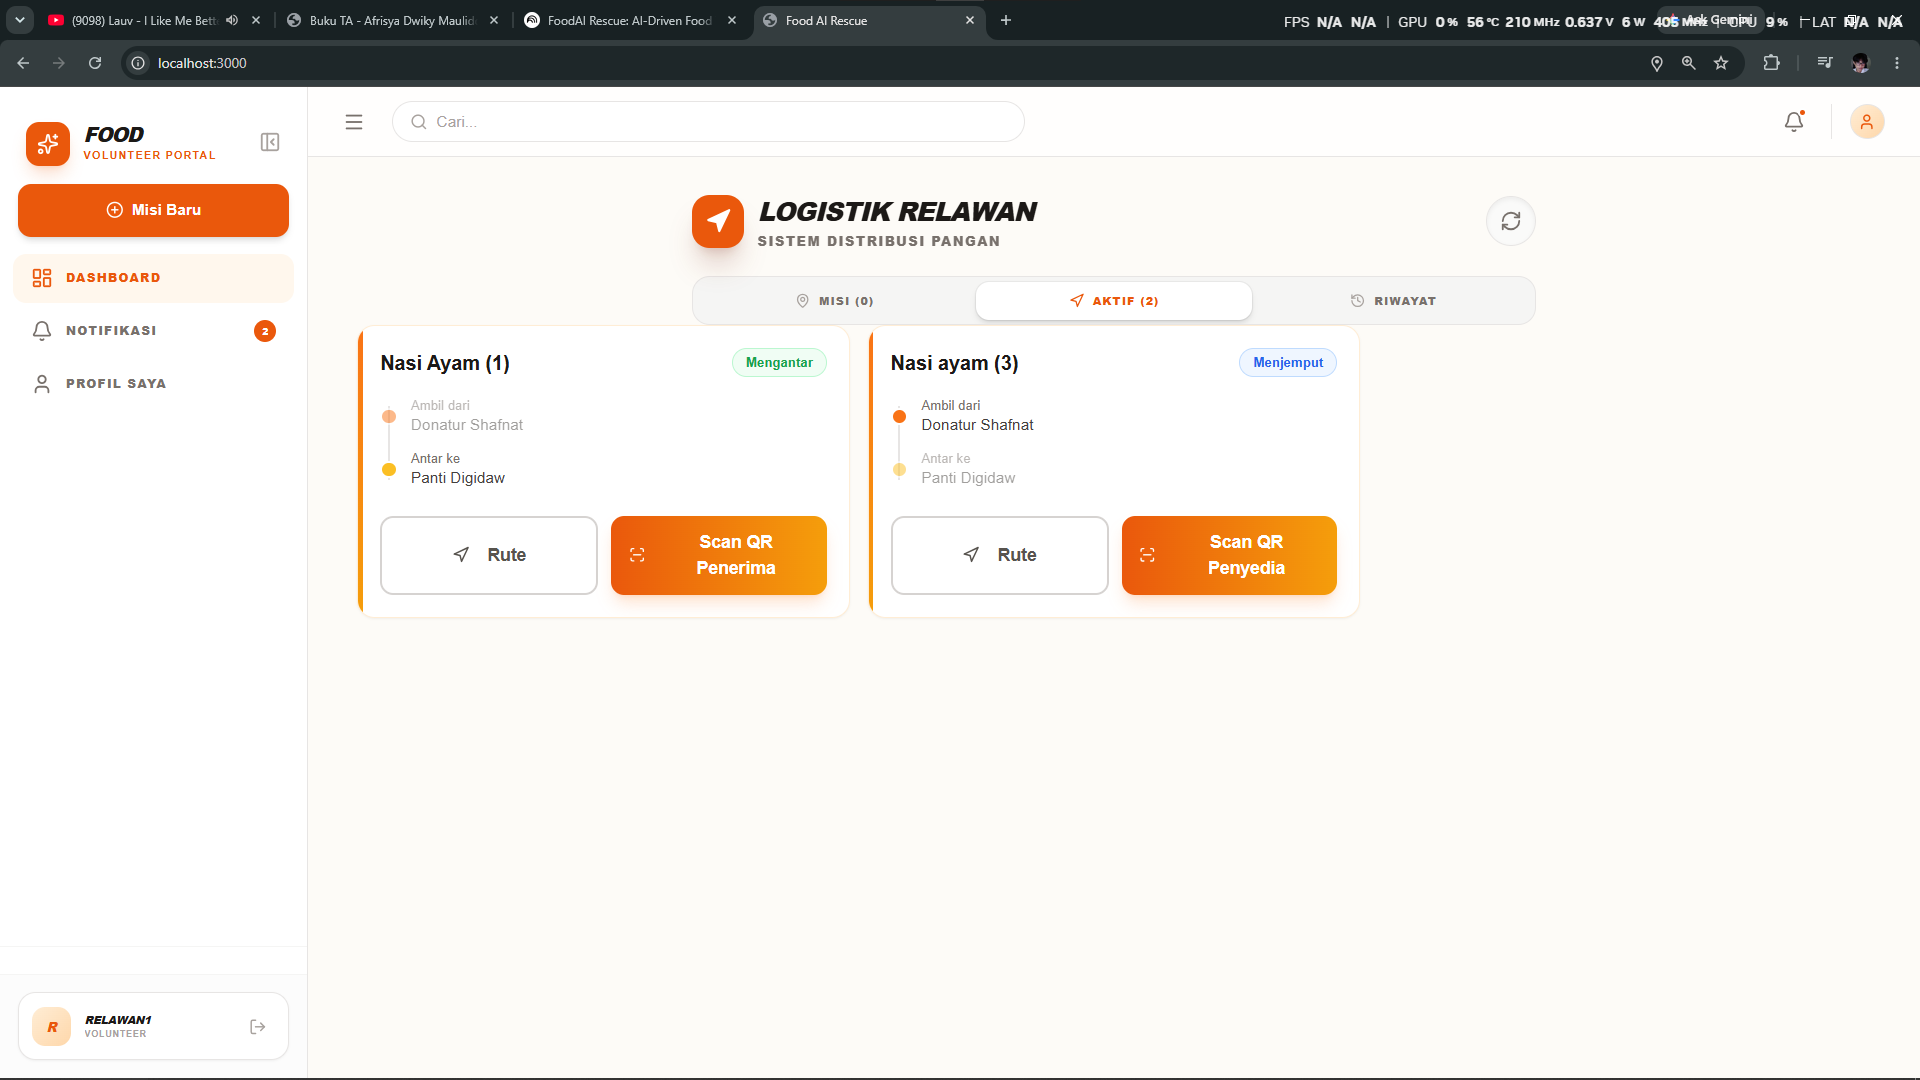
\includegraphics[width=\linewidth]{image/bab4/UserManual/TunjukQR/1-MisiAktif.png}
    \caption{Misi Aktif Logistik}
\end{figure}

\begin{figure}[H]
    \centering
    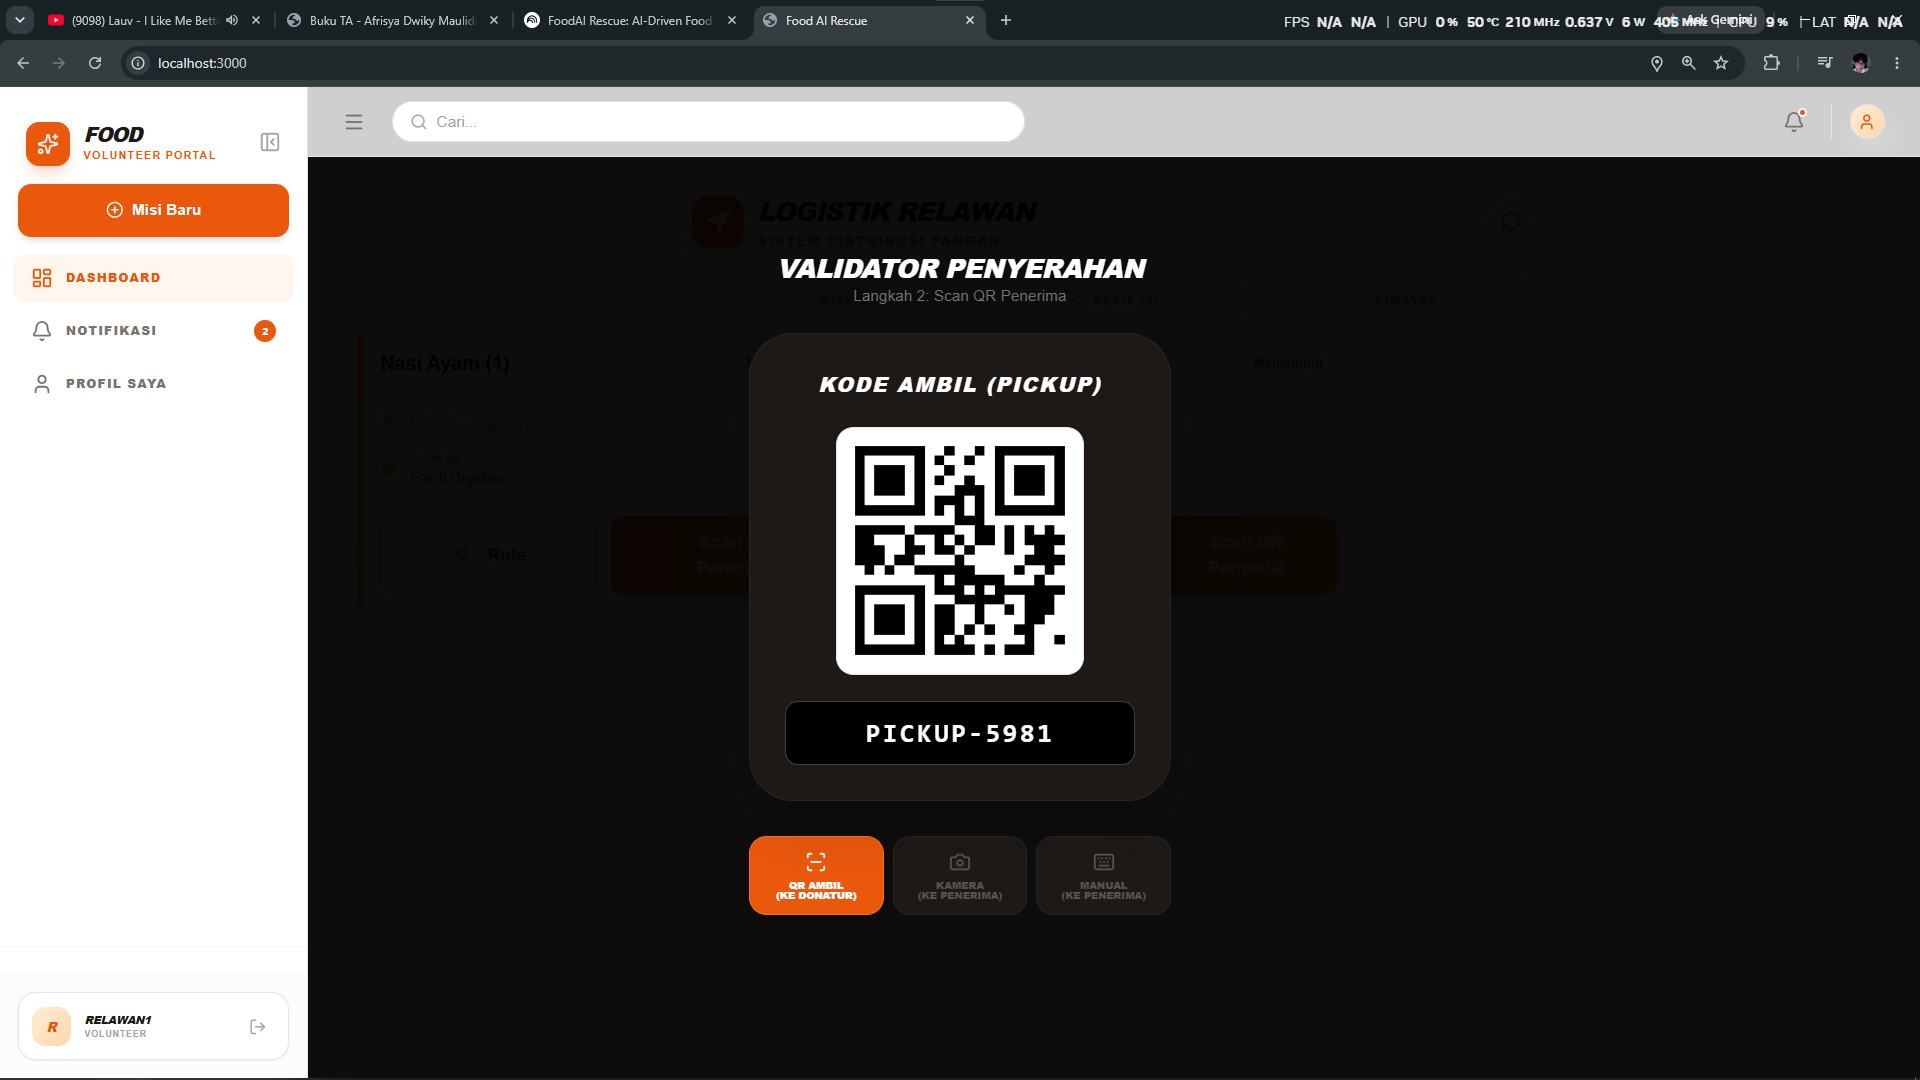
\includegraphics[width=\linewidth]{image/bab4/UserManual/TunjukQR/2-QRPickup.png}
    \caption{\textit{QR Code}}
\end{figure}



\subsubsection{Proses Verifikasi Penyerahan ke Penerima}
Langkah-langkah menyerahkan makanan secara nirkontak di titik tujuan akhir:
\begin{enumerate}[label=\arabic*.]
    \item Saat tiba di alamat penerima, buka kembali layar \textbf{Misi Aktif}.
    \item Tekan tombol verifikasi penerima untuk membuka pemindai kamera (\textit{Scan QR}), atau masukkan kode resi milik penerima melalui opsi \textit{Input Manual}.
\end{enumerate}

\begin{figure}[H]
    \centering
    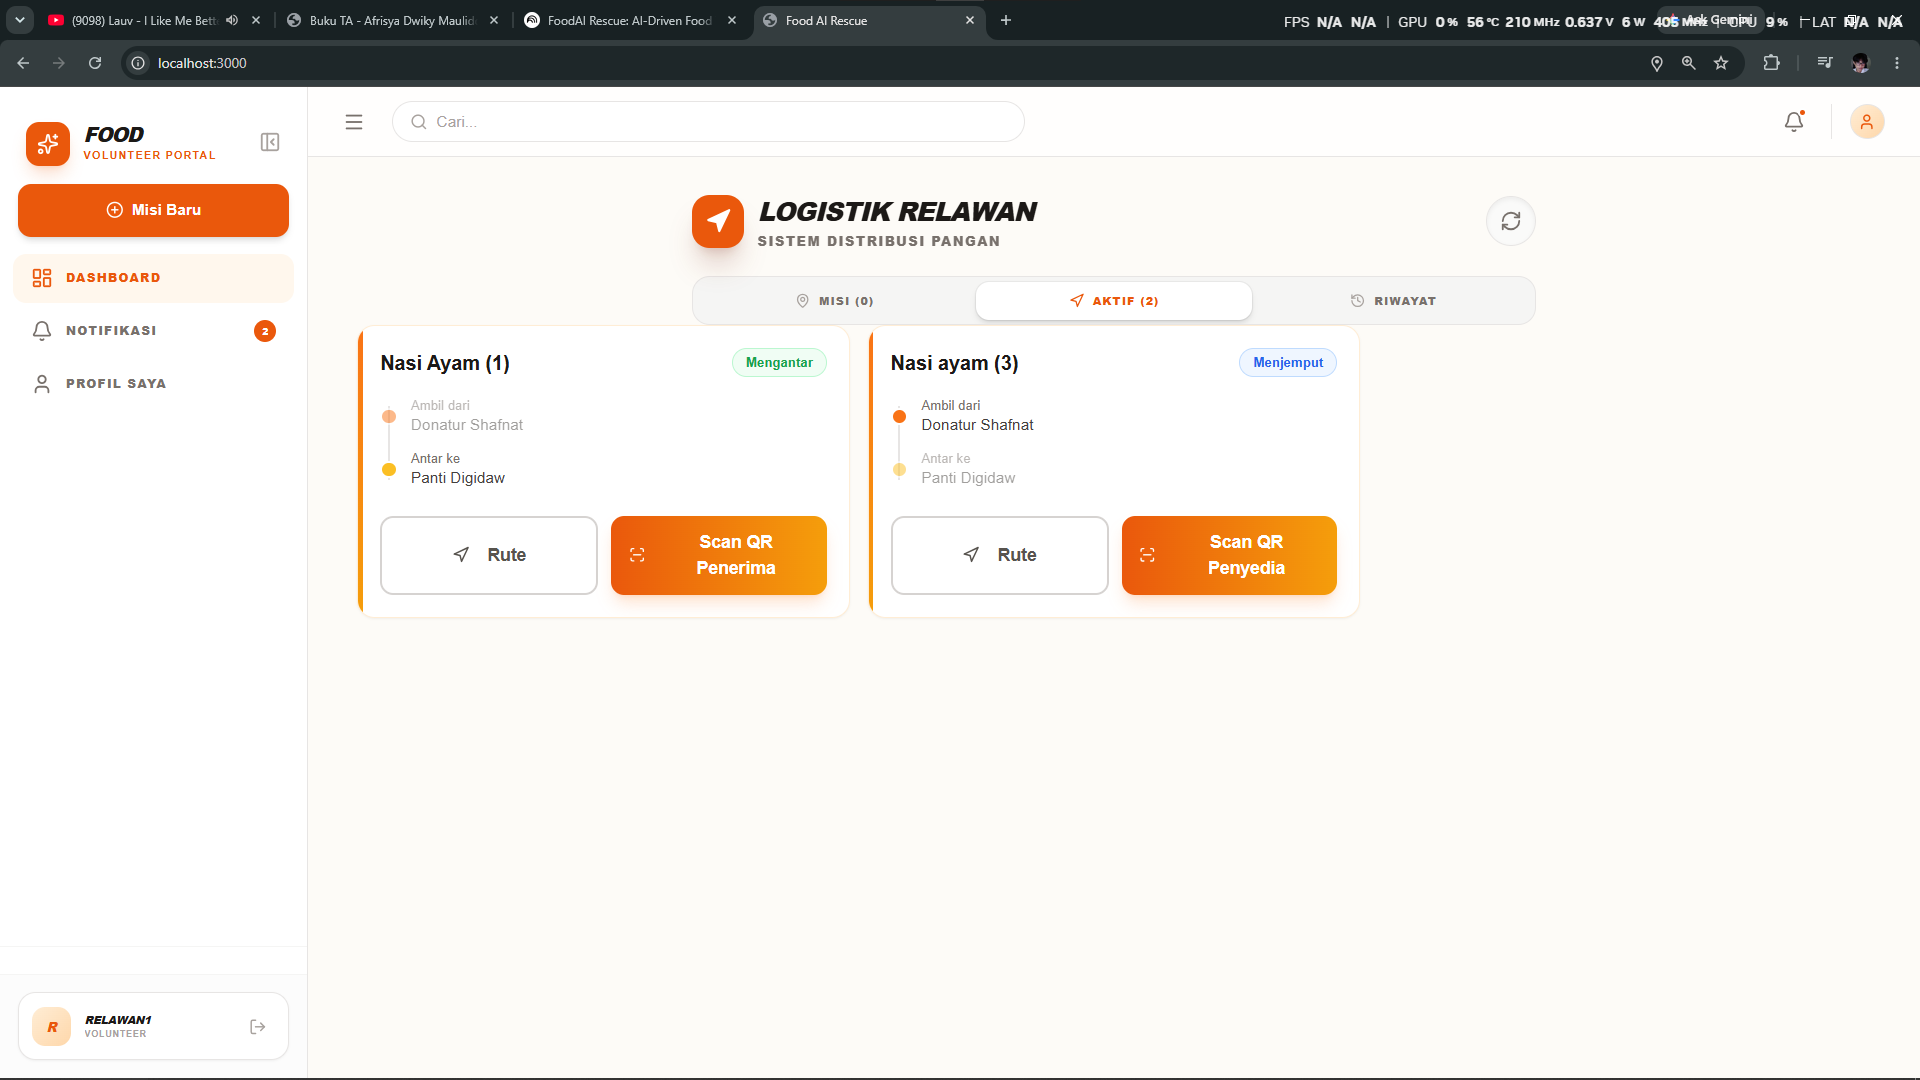
\includegraphics[width=\linewidth]{image/bab4/UserManual/VerifikasiPenerima/1-MisiAktifPengantaran.png}
    \caption{Misi Pengantaran Aktif}
\end{figure}

\begin{figure}[H]
    \centering
    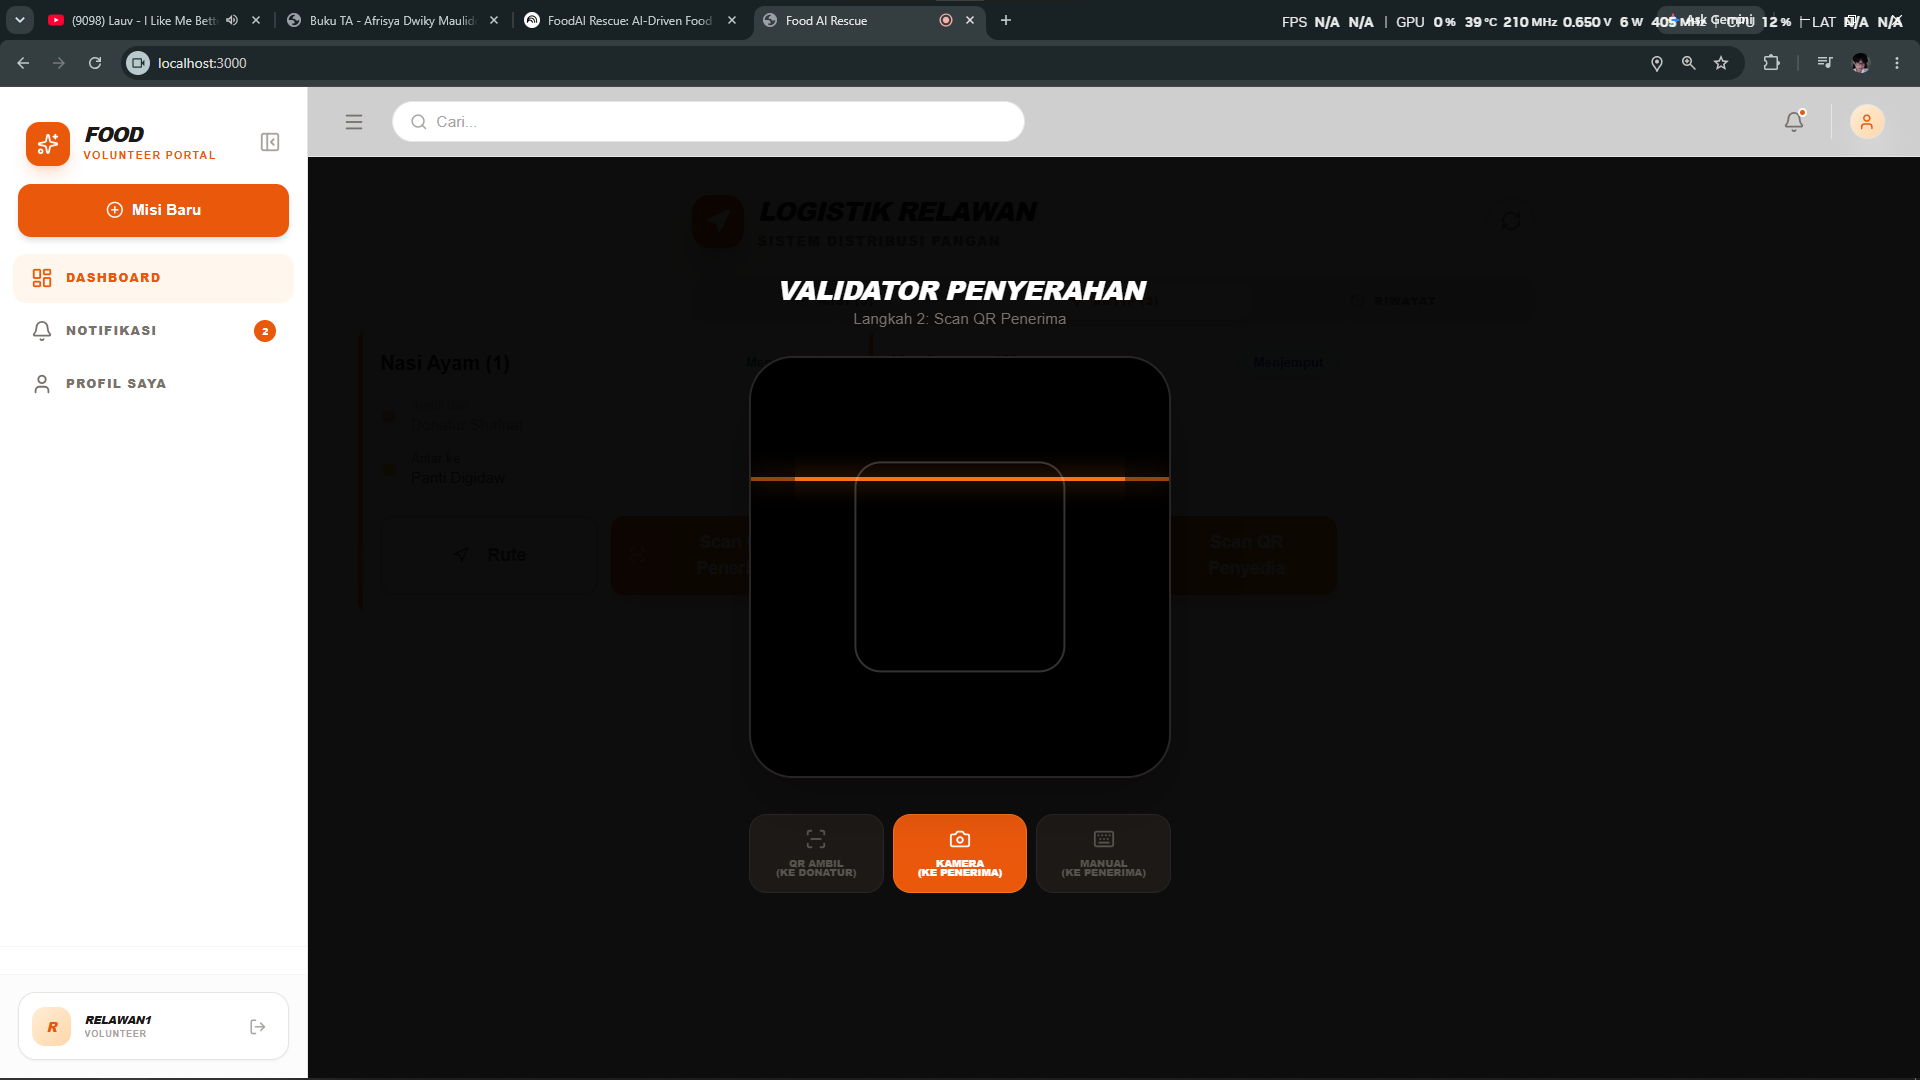
\includegraphics[width=\linewidth]{image/bab4/UserManual/VerifikasiPenerima/3-ScanQR.png}
    \caption{Memindai QR Penerima}
\end{figure}

\begin{figure}[H]
    \centering
    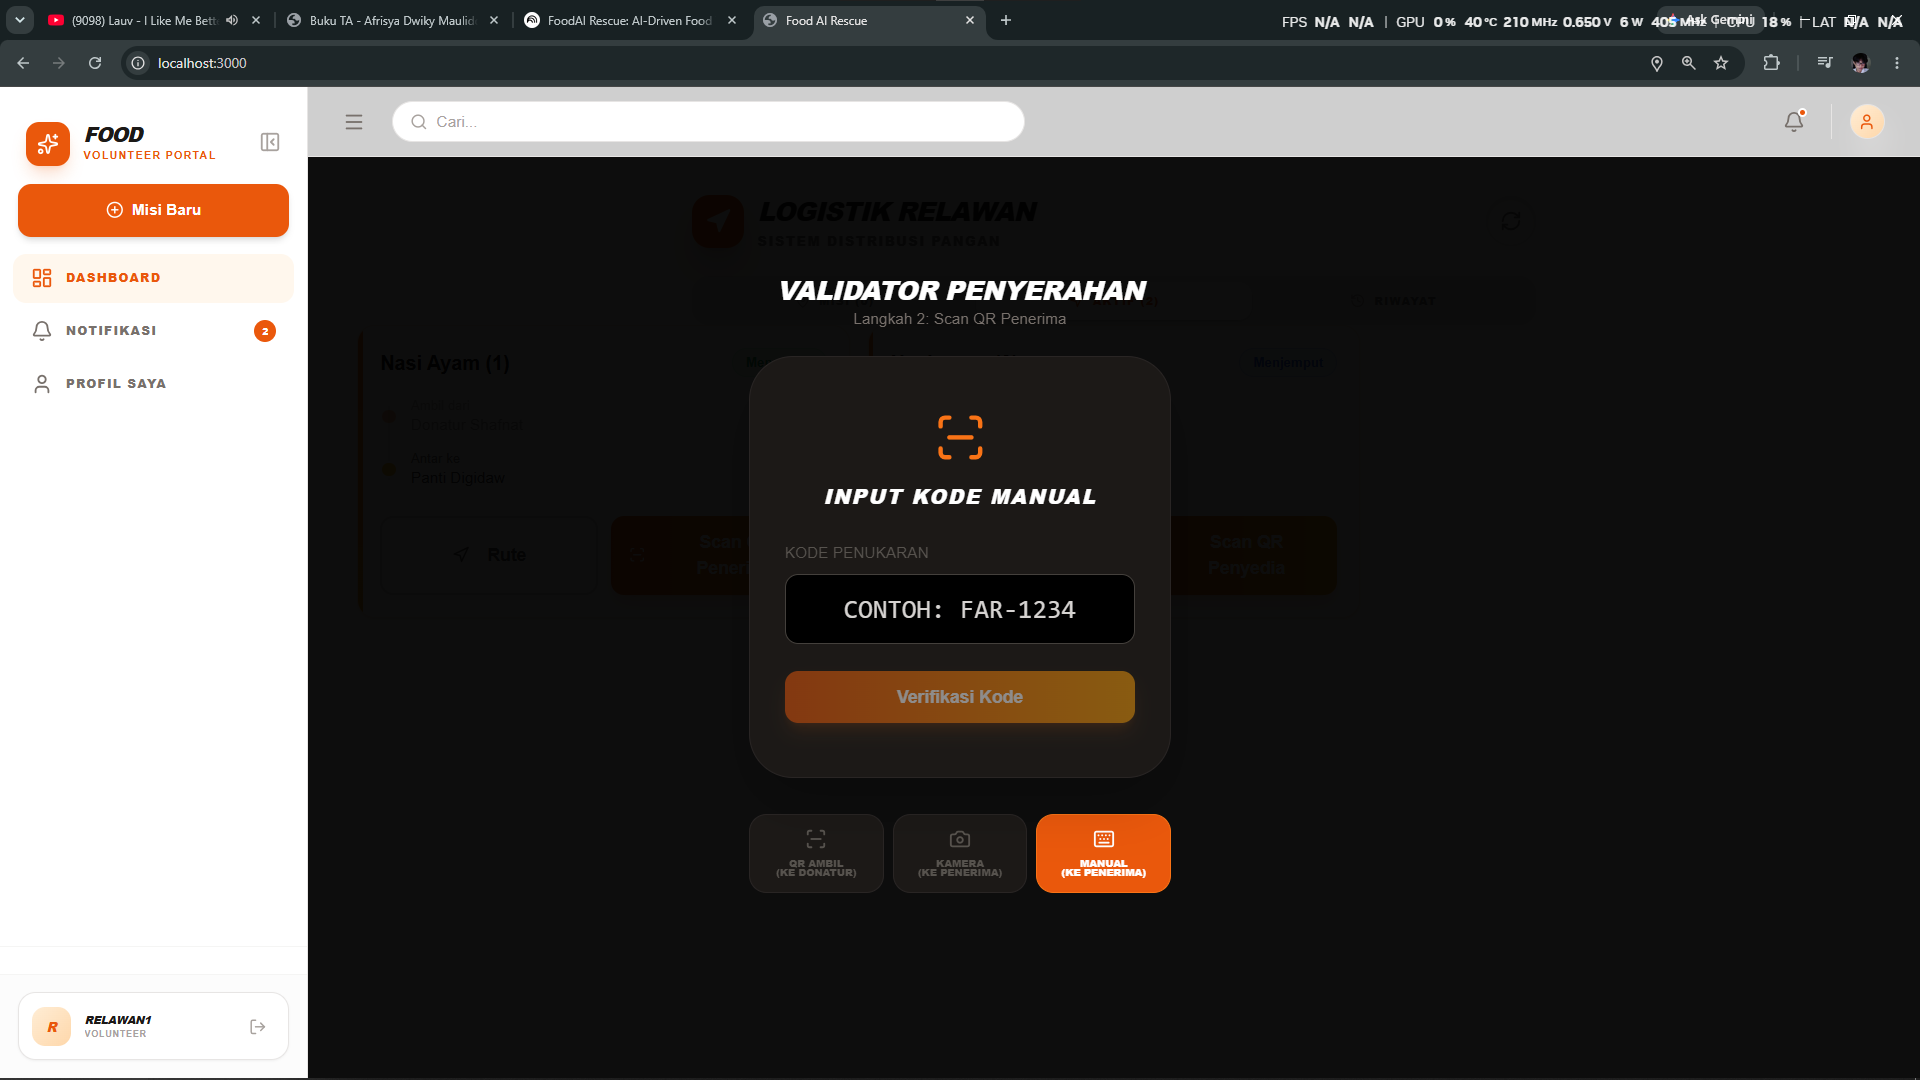
\includegraphics[width=\linewidth]{image/bab4/UserManual/VerifikasiPenerima/2-InputManual.png}
    \caption{Input Kode Manual}
\end{figure}



\section{Pengujian}

Pengujian pada platform FoodAI Rescue dieksekusi menggunakan metode \textit{Black-box Testing}. Metode ini dipilih karena berfokus pada evaluasi fungsionalitas antarmuka sistem---termasuk respons integrasi Kecerdasan Buatan (AI)---tanpa perlu menelusuri struktur internal atau kode sumber programnya. Teknik pengujian yang diterapkan juga disesuaikan dengan karakteristik fitur yang diuji, yang secara spesifik menitikberatkan pada penggunaan teknik \textit{Boundary Value Analysis} (BVA) dan \textit{Equivalence Partitioning} (EP).

Skenario pengujian otomasi dirancang untuk menyimulasikan interaksi dari berbagai target pengguna dengan batasan hak akses yang berbeda di dalam ekosistem aplikasi, meliputi:
\begin{enumerate}[label=\arabic*.]
    \item \textbf{Donatur (Individu dan Korporat)}: Skenario pengujian difokuskan pada simulasi pengunggahan surplus makanan, pencatatan titik jemput logistik, peninjauan Dasbor Dampak Sosial (SROI), serta fungsionalitas verifikasi gambar oleh AI "Polisi Pangan".
    \item \textbf{Penerima Donasi (Fasilitas Sosial/Masyarakat Rentan)}: Skenario pengujian menyimulasikan alur pencarian makanan pada peta ketersediaan (\textit{Radar}) hingga keberhasilan melakukan klaim (\textit{booking}) stok donasi.
    \item \textbf{Relawan (Kurir Logistik)}: Skenario pengujian ditujukan untuk menguji kapabilitas sistem dalam penerimaan misi pengantaran, validasi serah terima melalui pemindaian nirkontak (\textit{scan} QR Code), serta penambahan poin pengalaman (XP) pada sistem gamifikasi.
\end{enumerate}

Pendekatan pengujian berbasis simulasi multikomponen ini bertujuan untuk memastikan bahwa seluruh instrumen sistem mampu mengakomodasi kebutuhan interaksi yang saling berkaitan. Dengan menguji aplikasi dari berbagai sudut pandang otoritas pengguna---mulai dari hulu (penyediaan donasi) hingga hilir (distribusi akhir)---hasil pengujian diharapkan dapat secara komprehensif merefleksikan alur operasional di lapangan, memetakan potensi galat (\textit{bug}) sejak dini, dan menjamin keandalan sistem secara keseluruhan.




\subsection{Skenario Pengujian}
\textbf{a. Skenario 1 – Pembuktian Tujuan 1}

Untuk membuktikan ketercapaian Tujuan 1, yaitu “membangun platform penghubung logistik digital berbasis \textit{Progressive Web App} (PWA) untuk mendistribusikan surplus makanan dari donatur ke fasilitas sosial atau masyarakat rentan secara \textit{real-time} guna mencegah makanan tersebut membusuk menjadi sampah (\textit{food waste})”, maka dilakukan pengujian menggunakan metode \textit{Black-box Testing} dengan teknik \textit{Equivalence Partitioning}. Pengujian ini dieksekusi berdasarkan masukan data pada setiap formulir yang terdapat di antarmuka sistem aplikasi (seperti formulir registrasi, \textit{login}, dan unggah donasi). Setiap parameter masukan akan diuji dan dikelompokkan ke dalam beberapa partisi berdasarkan kesamaan fungsinya, guna memastikan sistem berfungsi dengan benar baik saat menerima data yang bernilai valid maupun tidak valid.

\begin{enumerate}[label=\arabic*.]
    \item \textbf{Validasi Autentikasi Pengguna (Registrasi dan \textit{Login}):}
    \begin{enumerate}[label=\alph*.]
        \item Memastikan pengguna dapat mendaftarkan akun baru dengan melengkapi data yang valid.
        \item Memastikan sistem menolak pendaftaran dan memberikan pesan galat (\textit{error}) apabila pengguna menggunakan alamat email yang sudah terdaftar atau jika konfirmasi kata sandi tidak cocok.
        \item Memastikan sistem memvalidasi kredensial saat \textit{login}, memberikan akses dasbor sesuai peran (\textit{role}) jika data valid, serta menolak akses jika kata sandi atau email yang dimasukkan salah.
    \end{enumerate}
    
    \item \textbf{Validasi Manajemen Unggah Donasi Makanan:}
    \begin{enumerate}[label=\alph*.]
        \item Memastikan donatur (individu maupun korporat) dapat mempublikasikan donasi makanan dengan mengisi kelengkapan formulir dan mengunggah foto yang valid.
        \item Memastikan sistem menggagalkan proses publikasi dan memberikan peringatan apabila donatur mengosongkan \textit{field} yang wajib diisi (seperti nama donasi).
        \item Memastikan sistem memvalidasi input numerik dengan menolak publikasi apabila donatur memasukkan kuantitas porsi donasi yang tidak valid (misalnya mengisi dengan angka 0).
    \end{enumerate}
    
    \item \textbf{Validasi Fungsionalitas Klaim dan Persetujuan Pesanan:}
    \begin{enumerate}[label=\alph*.]
        \item Memastikan pengguna dengan hak akses Penerima dapat mencari dan melakukan klaim pesanan pada makanan yang berstatus tersedia di dasbor mereka.
        \item Memastikan pengguna dengan hak akses Donatur menerima notifikasi pesanan masuk, serta dapat memproses pesanan tersebut dengan melakukan persetujuan (\textit{Terima Request}) agar statusnya berubah menjadi siap diambil, atau melakukan penolakan jika stok bermasalah.
    \end{enumerate}
\end{enumerate}

Guna mendukung kelancaran eksekusi pengujian secara terotomatisasi, skenario pengujian dirancang dengan mengklasifikasikan parameter data uji ke dalam kelas ekuivalen (bernilai valid maupun invalid). Adapun rincian skenario pengujian untuk mengevaluasi fungsionalitas utama sistem (Tujuan 1) dijabarkan pada tabel berikut:

\clearpage
\begin{landscape}
\pagestyle{lscape}
\begin{longtable}{|c|p{3cm}|p{3.5cm}|p{3.5cm}|p{3.5cm}|p{3cm}|p{3cm}|}
\caption{Skenario Pengujian Fitur Utama (Tujuan 1)}
\label{tab:skenario-tujuan1} \\
\hline
\rowcolor{gray!25}
\centering\textbf{Fungsio\-nalitas} & \centering\textbf{ID \textit{Test Case}} & \centering\textbf{Deskripsi/Skenario} & \centering\textbf{Pra Kondisi} & \centering\textbf{Langkah Pengujian} & \centering\textbf{Data Pengujian} & \centering\arraybackslash\textbf{Hasil yang Diharapkan} \\ \hline
\endfirsthead

\hline
\rowcolor{gray!25}
\centering\textbf{Fungsio\-nalitas} & \centering\textbf{ID \textit{Test Case}} & \centering\textbf{Deskripsi/Skenario} & \centering\textbf{Pra Kondisi} & \centering\textbf{Langkah Pengujian} & \centering\textbf{Data Pengujian} & \centering\arraybackslash\textbf{Hasil yang Diharapkan} \\ \hline
\endhead

\hline
\endfoot

\hline
\endlastfoot

% 1. Registrasi
\multirow{3}{2cm}{1. Registrasi} 
& TC1.1 & Pengguna mendaftar dengan data valid & Halaman utama pendaftaran & 1. Klik Daftar Gratis \newline 2. Pilih Peran \newline 3. Isi data lengkap \newline 4. Masukkan OTP & $\bullet$ Nama, email, password valid \newline $\bullet$ OTP sesuai & Registrasi berhasil, masuk ke dashboard \\ \cline{2-7}
& TC1.2 & Pengguna mendaftar dengan email yang sudah digunakan & Halaman utama pendaftaran & 1. Isi email yang terdaftar \newline 2. Klik Daftar & $\bullet$ Email sudah terdaftar & Registrasi gagal, pesan error email digunakan \\ \cline{2-7}
& TC1.3 & Pengguna mendaftar dengan konfirmasi password salah & Halaman utama pendaftaran & 1. Isi form \newline 2. Isi konfirmasi password berbeda & $\bullet$ Konfirmasi pass $\neq$ pass & Registrasi gagal, pesan error password salah \\ \hline

% 2. Login
\multirow{2}{2cm}{2. Login} 
& TC2.1 & Pengguna login dengan kredensial valid & Halaman Login & 1. Masukkan email \newline 2. Masukkan password \newline 3. Klik Masuk & $\bullet$ Email = valid \newline $\bullet$ Pass = valid & Login berhasil, diarahkan ke dashboard \\ \cline{2-7}
& TC2.2 & Pengguna login dengan password salah & Halaman Login & 1. Masukkan email \newline 2. Masukkan password \newline 3. Klik Masuk & $\bullet$ Email = valid \newline $\bullet$ Pass = salah & Login gagal, pesan error kredensial salah \\ \hline

% 3. Input Donasi
\multirow{3}{2cm}{3. Input Donasi} 
& TC3.1 & Donatur menambah donasi dengan data valid & Dashboard Donatur (Stok) & 1. Klik Tambah Donasi \newline 2. Isi kelengkapan \newline 3. Unggah foto \newline 4. Publikasikan & $\bullet$ Data valid, kuantitas $>$ 0, foto valid & Donasi berhasil dipublikasikan \\ \cline{2-7}
& TC3.2 & Donatur mengosongkan \textit{field} wajib & Dashboard Donatur (Stok) & 1. Kosongkan nama donasi \newline 2. Klik Publikasikan & $\bullet$ Nama = null & Publikasi gagal, peringatan field wajib \\ \cline{2-7}
& TC3.3 & Donatur memasukkan kuantitas donasi tidak valid & Dashboard Donatur (Stok) & 1. Isi kuantitas nol \newline 2. Klik Publikasikan & $\bullet$ Kuantitas = 0 & Publikasi gagal, peringatan kuantitas \\ \hline

% 4. Claim Donasi
4. Claim Donasi & TC4.1 & Penerima mengklaim donasi yang tersedia & Dashboard Penerima & 1. Pilih donasi \newline 2. Klik Klaim Sekarang \newline 3. Ya, Yakin & $\bullet$ Stok donasi $>$ 0 & Klaim berhasil, tiket klaim dibuat \\ \hline

% 5. Terima Request
\multirow{2}{2cm}{5. Terima Request} 
& TC5.1 & Donatur menyetujui \textit{request} klaim & Dashboard Donatur (Pesanan) & 1. Detail Pesanan \newline 2. Klik Setujui & $\bullet$ Ada pesanan aktif & Request disetujui, pesanan diproses \\ \cline{2-7}
& TC5.2 & Donatur menolak \textit{request} klaim & Dashboard Donatur (Pesanan) & 1. Detail Pesanan \newline 2. Klik Tolak & $\bullet$ Alasan = stok rusak & Request ditolak, pesanan dibatalkan \\ \hline

\end{longtable}
\pagestyle{fancy}
\end{landscape}
\clearpage

\textbf{2) Cakupan Pengujian Skenario 2}

Pengujian pada skenario ini dirancang untuk membuktikan ketercapaian Tujuan 2 pada aspek keamanan pangan, yakni mengevaluasi keandalan integrasi model Kecerdasan Buatan (Google Gemini Vision API) dalam memvalidasi kelayakan surplus makanan secara visual (\textit{Polisi Pangan}). Mengingat pengujian difokuskan pada alur kerja utama distribusi logistik, evaluasi penerapan AI Generatif untuk kampanye korporat tidak dimasukkan dalam skenario ini. Dengan menerapkan teknik \textit{Equivalence Partitioning} (EP), cakupan pengujian pada modul "Polisi Pangan" meliputi:

\begin{enumerate}[label=\arabic*.]
    \item \textbf{Validasi Visual Kelayakan Donasi Makanan:}
    \begin{enumerate}[label=\alph*.]
        \item Memastikan sistem dapat terintegrasi dengan antarmuka AI untuk memproses unggahan foto makanan dari donatur secara \textit{real-time} saat proses pengisian formulir donasi.
        \item Memastikan algoritma AI mampu menyetujui publikasi donasi (masuk ke dalam katalog ketersediaan) apabila gambar yang diunggah dinilai aman, higienis, dan masuk dalam partisi ekuivalensi data valid.
        \item Memastikan sistem secara otonom dapat mendeteksi, menolak publikasi, dan memberikan peringatan (notifikasi galat) apabila donatur mengunggah gambar yang tidak relevan (misalnya benda mati/objek acak) atau makanan yang secara visual terindikasi tidak layak konsumsi, guna memastikan keamanan pangan bagi penerima di hilir.
    \end{enumerate}
\end{enumerate}

\clearpage
\begin{landscape}
\pagestyle{lscape}
\begin{longtable}{|c|p{3cm}|p{3.5cm}|p{3.5cm}|p{3.5cm}|p{3cm}|p{3cm}|}
\caption{Skenario Pengujian Verifikasi AI (Tujuan 2)}
\label{tab:skenario-tujuan2} \\
\hline
\rowcolor{gray!25}
\centering\textbf{Fungsio\-nalitas} & \centering\textbf{ID \textit{Test Case}} & \centering\textbf{Deskripsi/Skenario} & \centering\textbf{Pra Kondisi} & \centering\textbf{Langkah Pengujian} & \centering\textbf{Data Pengujian} & \centering\arraybackslash\textbf{Hasil yang Diharapkan} \\ \hline
\endfirsthead

\hline
\rowcolor{gray!25}
\centering\textbf{Fungsio\-nalitas} & \centering\textbf{ID \textit{Test Case}} & \centering\textbf{Deskripsi/Skenario} & \centering\textbf{Pra Kondisi} & \centering\textbf{Langkah Pengujian} & \centering\textbf{Data Pengujian} & \centering\arraybackslash\textbf{Hasil yang Diharapkan} \\ \hline
\endhead

\hline
\endfoot

\hline
\endlastfoot

% Audit Foto AI
\multirow{3}{2cm}{Polisi Pangan (Audit AI)} 
& TC-AI.1 & Memvalidasi foto makanan layak konsumsi & Formulir Input Donasi & 1. Unggah foto makanan \newline 2. Sistem memanggil API AI \newline 3. Tampilkan hasil & $\bullet$ Foto makanan utuh dan higienis & AI memberikan skor tinggi, donasi disetujui masuk katalog \\ \cline{2-7}
& TC-AI.2 & Memvalidasi foto objek benda mati & Formulir Input Donasi & 1. Unggah foto objek acak \newline 2. Sistem memanggil API AI \newline 3. Tampilkan hasil & $\bullet$ Foto bukan makanan (objek acak) & AI gagal identifikasi komposisi, publikasi ditolak, muncul galat \\ \cline{2-7}
& TC-AI.3 & Memvalidasi foto makanan tidak layak & Formulir Input Donasi & 1. Unggah foto basi/berjamur \newline 2. Sistem memanggil API AI \newline 3. Tampilkan hasil & $\bullet$ Foto makanan kotor/berjamur & AI mendeteksi ketidaklayakan (skor rendah), publikasi diblokir \\ \hline
\end{longtable}
\pagestyle{fancy}
\end{landscape}
\clearpage

\textbf{c. Skenario 3 – Pembuktian Tujuan 3}

Untuk membuktikan ketercapaian Tujuan 3, yaitu “mengintegrasikan sistem gamifikasi (\textit{leaderboard}), pemindaian Kode QR nirkontak (\textit{contactless}), dan Dasbor Dampak Sosial (SROI) untuk memotivasi partisipasi relawan kurir, mencegah penyalahgunaan klaim ganda saat serah terima di lapangan, dan melacak pencapaian reduksi emisi karbon secara transparan”, maka dilakukan pengujian menggunakan metode \textit{Black-box Testing} dengan teknik \textit{Boundary Value Analysis} (BVA). Pengujian ini merupakan salah satu teknik evaluasi \textit{black-box} yang dirancang secara khusus untuk mengidentifikasi batasan nilai masukan yang krusial dengan menguji titik batas minimum dan maksimum. Pada ekosistem FoodAI Rescue, pengujian ini difokuskan pada batasan nilai numerik yang esensial, seperti batasan input kuantitas porsi donasi makanan (misalnya menginput 0 porsi, angka minus, atau batas maksimal porsi), serta perhitungan poin \textit{Experience} (XP) relawan. Hal ini dilakukan untuk memastikan bahwa logika kalkulasi pada sistem gamifikasi dan dasbor pelacakan dampak sosial (SROI) bekerja secara akurat dan terhindar dari galat manipulasi angka.

\begin{enumerate}[label=\arabic*.]
    \item \textbf{Validasi Manajemen Misi Logistik (Relawan):}
    \begin{enumerate}[label=\alph*.]
        \item Memastikan pengguna dengan hak akses Relawan dapat mengakses dasbor \textit{Missions Board}, melihat detail lokasi, dan berhasil mengklaim (mengambil) misi pengantaran logistik yang berstatus tersedia.
        \item Memastikan relawan dapat membatalkan misi yang telah diambil secara wajar (selama belum diproses lebih lanjut), dan sistem akan secara otomatis mengembalikan misi tersebut ke dalam katalog agar dapat direbut oleh relawan lain.
    \end{enumerate}

    \item \textbf{Validasi Serah Terima Nirkontak (Integrasi Kode QR):}
    \begin{enumerate}[label=\alph*.]
        \item Memastikan relawan mampu memunculkan Kode QR di perangkatnya untuk dipindai oleh donatur, dan memastikan donatur dapat menyetujui serah terima tahap pertama (hulu) menggunakan pemindaian atau input resi manual yang valid.
        \item Memastikan relawan dapat memindai Kode QR milik penerima donasi di titik lokasi tujuan untuk menyelesaikan transaksi distribusi logistik tahap akhir (hilir) apabila kode yang dimasukkan valid.
        \item Memastikan sistem secara tegas menolak, menggagalkan proses serah terima, dan menampilkan peringatan galat (\textit{error}) apabila pengguna (baik donatur maupun relawan) memindai atau memasukkan kode unik buatan yang salah/tidak valid, guna mencegah manipulasi, salah sasaran, maupun klaim ganda.
    \end{enumerate}

    \item \textbf{Validasi Akurasi Gamifikasi dan Dasbor SROI:}
    \begin{enumerate}[label=\alph*.]
        \item Memastikan sistem secara otomatis dan \textit{real-time} menambahkan poin \textit{Experience} (XP) kepada akun relawan sesaat setelah validasi Kode QR penerima dinyatakan sukses, yang memicu pembaruan posisi pada papan peringkat (\textit{Leaderboard}).
        \item Memastikan sistem pada Dasbor Dampak Sosial (SROI) mampu mengakumulasi dan merender grafik kalkulasi konversi secara presisi—dari jumlah porsi makanan yang terselamatkan menjadi data metrik estimasi penghematan air (liter) dan reduksi emisi jejak karbon (kg CO$_2$).
    \end{enumerate}
\end{enumerate}

\clearpage
\begin{landscape}
\pagestyle{lscape}
\begin{longtable}{|c|p{3cm}|p{3.5cm}|p{3.5cm}|p{3.5cm}|p{3cm}|p{3cm}|}
\caption{Skenario Pengujian Operasional Logistik dan Verifikasi (Tujuan 3)}
\label{tab:skenario-tujuan3} \\
\hline
\rowcolor{gray!25}
\centering\textbf{Fungsio\-nalitas} & \centering\textbf{ID \textit{Test Case}} & \centering\textbf{Deskripsi/Skenario} & \centering\textbf{Pra Kondisi} & \centering\textbf{Langkah Pengujian} & \centering\textbf{Data Pengujian} & \centering\arraybackslash\textbf{Hasil yang Diharapkan} \\ \hline
\endfirsthead

\hline
\rowcolor{gray!25}
\centering\textbf{Fungsio\-nalitas} & \centering\textbf{ID \textit{Test Case}} & \centering\textbf{Deskripsi/Skenario} & \centering\textbf{Pra Kondisi} & \centering\textbf{Langkah Pengujian} & \centering\textbf{Data Pengujian} & \centering\arraybackslash\textbf{Hasil yang Diharapkan} \\ \hline
\endhead

\hline
\endfoot

\hline
\endlastfoot

% 6. Ambil Misi
\multirow{2}{2cm}{6. Ambil Misi} 
& TC6.1 & Relawan mengambil misi pengantaran & Dashboard Relawan & 1. Detail Misi \newline 2. Ambil Misi Ini & $\bullet$ Misi status tersedia & Misi berhasil diambil relawan \\ \cline{2-7}
& TC6.3 & Relawan membatalkan misi yang diambil & Dashboard Relawan & 1. Buka misi aktif \newline 2. Batalkan Misi & $\bullet$ Misi belum diproses & Misi berhasil dibatalkan \\ \hline

% 7. Menunjukkan QR
7. Tunjuk QR & TC7.1 & Relawan menampilkan QR ke donatur & Dashboard Relawan & 1. Buka misi aktif \newline 2. Klik QR Ambil & $\bullet$ Relawan di tahap ambil & QR berhasil ditampilkan \\ \hline

% 8. Scan QR
\multirow{2}{2cm}{8. Scan QR} 
& TC8.1 & Donatur verifikasi resi manual relawan dengan benar & Dashboard Donatur & 1. Verifikasi Manual \newline 2. Input resi \newline 3. Verifikasi & $\bullet$ Kode = PICKUP-9800 & Verifikasi berhasil, makanan diserahkan \\ \cline{2-7}
& TC8.3 & Donatur memasukkan resi manual yang salah & Dashboard Donatur & 1. Verifikasi Manual \newline 2. Input resi \newline 3. Verifikasi & $\bullet$ Kode = PICKUP-0000 & Verifikasi gagal, muncul peringatan \\ \hline

% 9. Verifikasi
\multirow{2}{2cm}{9. Verifikasi Penerima} 
& TC9.1 & Relawan memasukkan kode penerima yang benar & Dashboard Relawan & 1. Buka Scan QR Penerima \newline 2. Input kode \newline 3. Verifikasi & $\bullet$ Kode = FAR-5089 & Verifikasi berhasil, misi selesai \\ \cline{2-7}
& TC9.2 & Relawan memasukkan kode penerima yang salah & Dashboard Relawan & 1. Buka Scan QR Penerima \newline 2. Input kode \newline 3. Verifikasi & $\bullet$ Kode = FAR-0000 & Verifikasi gagal, peringatan kode salah \\ \hline
\end{longtable}
\pagestyle{fancy}
\end{landscape}
\clearpage


\subsection{Hasil Pengujian}

Tahapan ini memaparkan hasil evaluasi dari eksekusi rancangan pengujian (\textit{test case}) yang telah disusun sebelumnya. Pengujian fungsionalitas sistem dieksekusi menggunakan perangkat lunak otomasi Katalon Studio. Hasil aktual dari respons antarmuka dan sistem \textit{backend} dikomparasikan dengan ekspektasi hasil untuk menentukan status keberhasilan. Skenario dinyatakan \textbf{\textit{Pass}} (Berhasil) apabila respons sistem sejalan dengan ekspektasi, dan dinyatakan \textbf{\textit{Failed}} (Gagal) apabila ditemukan galat (\textit{bug}) atau ketidaksesuaian validasi pada sistem.

\textbf{a. Hasil Pengujian Skenario 1 (Pembuktian Tujuan 1)}

Pengujian pada tahap ini difokuskan pada alur kerja utama aplikasi (\textit{core business flow}), mulai dari pendaftaran akun, autentikasi, penyediaan donasi, hingga proses klaim pesanan.

\begin{table}[H]
\centering
\caption{Hasil Pengujian Fitur Utama (Tujuan 1)}
\label{tab:hasil-tujuan1}
\begin{tabularx}{\textwidth}{|c|L|L|L|c|}
\hline
\rowcolor{gray!25}
\textbf{ID} & \textbf{Fitur yang Diuji} & \textbf{Langkah Pengujian (Simulasi Sistem)} & \textbf{Hasil Aktual Sistem} & \textbf{Status} \\ \hline
\textbf{TC1.1} & Registrasi (Valid) & Sistem menyimulasikan pengisian formulir daftar (nama, email baru, \textit{password}, nomor WA) dan menekan tombol "Daftar". & Akun berhasil dibuat dan pengguna langsung diarahkan ke \textit{Dashboard}. & \textbf{Pass} \\ \hline
\textbf{TC1.2} & Registrasi (Email Duplikat) & Sistem menyimulasikan pendaftaran menggunakan alamat email yang sudah pernah terdaftar di basis data. & Sistem menolak pendaftaran dan memunculkan peringatan "Email sudah digunakan". & \textbf{Pass} \\ \hline
\textbf{TC1.3} & Registrasi (Sandi Tidak Cocok) & Sistem menginputkan kata sandi utama dan konfirmasi kata sandi yang berbeda. & Sistem menggagalkan proses dan memunculkan peringatan validasi \textit{password}. & \textbf{Pass} \\ \hline
\textbf{TC2.1} & Login (Valid) & Sistem menginputkan email dan kata sandi yang benar, lalu menekan tombol "Masuk". & Autentikasi berhasil, pengguna dialihkan ke Dasbor sesuai perannya (\textit{Role}). & \textbf{Pass} \\ \hline
\textbf{TC2.2} & Login (Invalid) & Sistem menginputkan kombinasi email atau kata sandi yang salah/tidak terdaftar. & Autentikasi ditolak, muncul peringatan galat "Kredensial salah". & \textbf{Pass} \\ \hline
\textbf{TC3.1} & Input Donasi (Valid) & Donatur mengisi lengkap data makanan, mengunggah foto, dan memublikasikannya. & Data terkirim ke \textit{backend}, divalidasi, dan donasi berhasil masuk ke katalog. & \textbf{Pass} \\ \hline
\textbf{TC3.2} & Input Donasi (Field Kosong) & Donatur sengaja mengosongkan \textit{field} wajib (seperti nama donasi) dan mencoba menyimpan. & Sistem \textbf{gagal} memblokir proses penyimpanan, peringatan validasi tidak muncul secara tepat. & \textbf{Failed} \\ \hline
\textbf{TC3.3} & Input Donasi (Kuantitas Nol) & Donatur memasukkan angka 0 pada jumlah porsi makanan. & Sistem \textbf{gagal} menolak input batas bawah (BVA), sehingga donasi dengan porsi 0 lolos. & \textbf{Failed} \\ \hline
\textbf{TC4.1} & Klaim Donasi & Penerima mencari makanan di katalog, mengatur lokasi, dan menekan "Klaim Sekarang". & Transaksi klaim berhasil dibuat dan status stok makanan terkunci. & \textbf{Pass} \\ \hline
\textbf{TC5.1} & Terima Pesanan & Donatur membuka riwayat pesanan masuk dan menekan tombol "Setujui". & Status pesanan diperbarui menjadi "Siap Diambil" oleh sistem. & \textbf{Pass} \\ \hline
\textbf{TC5.2} & Tolak Pesanan & Donatur menekan tombol "Tolak" karena alasan stok bermasalah. & Pesanan berhasil dibatalkan dan dikembalikan statusnya. & \textbf{Pass} \\ \hline
\end{tabularx}
\end{table}

\textbf{b. Hasil Pengujian Skenario 2 (Pembuktian Tujuan 2)}

Pengujian ini berfokus pada ketangguhan validasi integrasi \textit{Google Gemini Vision API} yang bertindak sebagai "Polisi Pangan" saat donatur mengunggah foto makanan.

\begin{table}[H]
\centering
\caption{Hasil Pengujian Verifikasi AI (Tujuan 2)}
\label{tab:hasil-tujuan2}
\begin{tabularx}{\textwidth}{|c|L|L|L|c|}
\hline
\rowcolor{gray!25}
\textbf{ID} & \textbf{Fitur yang Diuji} & \textbf{Langkah Pengujian (Simulasi Sistem)} & \textbf{Hasil Aktual Sistem} & \textbf{Status} \\ \hline
\textbf{TC-AI.1} & Audit AI (Foto Valid) & Mengunggah foto makanan utuh dan menekan tombol "Lanjut ke Foto Audit AI". & AI mengekstraksi skor keamanan tinggi dan menyetujui publikasi donasi. & \textbf{Pass} \\ \hline
\textbf{TC-AI.2} & Audit AI (Bukan Makanan) & Mengunggah foto objek acak (benda mati) untuk menguji \textit{Clever Hans effect}. & AI gagal mendeteksi komposisi makanan dan menolak proses publikasi. & \textbf{Pass} \\ \hline
\textbf{TC-AI.3} & Audit AI (Tidak Layak) & Mengunggah foto makanan berjamur/kotor. & AI memberikan skor keamanan rendah dan memblokir publikasi. & \textbf{Pass} \\ \hline
\end{tabularx}
\end{table}

\textit{(Catatan: Kode TC-AI.x ditambahkan khusus untuk Buku TA guna menjelaskan apa yang terjadi di balik layar saat skrip Katalon Anda menekan tombol "Lanjut ke Foto Audit AI" pada skenario input donasi).}

\textbf{c. Hasil Pengujian Skenario 3 (Pembuktian Tujuan 3)}

Pengujian ini mengevaluasi keandalan operasional logistik di lapangan, keamanan sistem pindai Kode QR secara nirkontak, serta pemicu (\textit{trigger}) ke sistem poin gamifikasi.

\begin{table}[H]
\centering
\caption{Hasil Pengujian Logistik dan Verifikasi (Tujuan 3)}
\label{tab:hasil-tujuan3}
\begin{tabularx}{\textwidth}{|c|L|L|L|c|}
\hline
\rowcolor{gray!25}
\textbf{ID} & \textbf{Fitur yang Diuji} & \textbf{Langkah Pengujian (Simulasi Sistem)} & \textbf{Hasil Aktual Sistem} & \textbf{Status} \\ \hline
\textbf{TC6.1} & Ambil Misi Logistik & Relawan membuka \textit{Missions Board} dan menekan tombol "Ambil Misi Ini". & Misi berhasil ditugaskan ke relawan dan rute penjemputan ditampilkan. & \textbf{Pass} \\ \hline
\textbf{TC6.2} & Batal Misi & Relawan menekan tombol "Batalkan Misi" sebelum diproses lebih lanjut. & Misi dilepas dan dikembalikan ke daftar agar bisa diambil relawan lain. & \textbf{Pass} \\ \hline
\textbf{TC7.1} & Generate QR Code & Relawan menekan tombol "QR Ambil" saat tiba di lokasi donatur. & Sistem berhasil merender Kode QR unik milik relawan di layar. & \textbf{Pass} \\ \hline
\textbf{TC8.1} & Verifikasi Penjemputan (Valid) & Donatur memindai atau menginput resi nirkontak relawan dengan kode yang \textbf{benar}. & Verifikasi sukses, makanan sah diserahkan ke relawan, misi berlanjut. & \textbf{Pass} \\ \hline
\textbf{TC8.3} & Verifikasi Penjemputan (Invalid) & Donatur memasukkan resi dengan kode acak/salah (misal: \texttt{PICKUP-0000}). & Sistem menolak serah terima dan memunculkan peringatan kode salah. & \textbf{Pass} \\ \hline
\textbf{TC9.1} & Verifikasi Pengantaran (Valid) & Relawan tiba di lokasi tujuan dan menginput kode unik penerima yang \textbf{benar}. & Verifikasi sukses, transaksi selesai (\textit{Completed}), dan poin Gamifikasi bertambah. & \textbf{Pass} \\ \hline
\textbf{TC9.2} & Verifikasi Pengantaran (Invalid) & Relawan memasukkan kode penerima yang salah (misal: \texttt{FAR-0000}). & Verifikasi gagal, sistem mencegah penyelesaian misi untuk menghindari salah sasaran. & \textbf{Pass} \\ \hline
\end{tabularx}
\end{table}



\chapter{PENUTUP}
\label{chapter:PENUTUP}

\section{Kesimpulan}

Berdasarkan hasil perancangan, implementasi (pengkodean), dan pengujian perangkat lunak yang telah dipaparkan pada bab-bab sebelumnya, dapat ditarik kesimpulan bahwa platform FoodAI Rescue (FAR) telah berhasil dibangun sebagai solusi digital terpadu untuk mengatasi permasalahan manajemen donasi surplus makanan. Kesimpulan ini secara spesifik menjawab rumusan masalah dan tujuan yang telah ditetapkan:

\begin{enumerate}[label=\arabic*.]
    \item \textbf{Keberhasilan Pembangunan Alur Logistik Digital}: Platform agregator logistik berbasis \textit{Progressive Web App} (PWA) dengan arsitektur \textit{Role-Based Access Control} (RBAC) yang membagi pengguna ke dalam 6 peran telah berhasil diimplementasikan. Pengujian fungsionalitas (\textit{Black-box Testing}) membuktikan bahwa proses dari hulu ke hilir, mulai dari registrasi, publikasi donasi oleh donatur, hingga pencarian dan klaim oleh penerima, dapat berjalan secara \textit{real-time}. Sistem secara efektif menjembatani distribusi surplus makanan agar tidak membusuk menjadi \textit{food waste} di Tempat Pembuangan Akhir (TPA). Meskipun demikian, berdasarkan pengujian \textit{Boundary Value Analysis}, masih ditemukan celah kecil pada validasi input \textit{frontend} yang meloloskan kuantitas bernilai nol.
    \item \textbf{Keandalan Validasi "Polisi Pangan" AI}: Implementasi teknologi \textit{Computer Vision} yang mendayagunakan Google Gemini Vision API telah sukses terintegrasi sebagai "Polisi Pangan". Pengujian partisi ekuivalen (\textit{Equivalence Partitioning}) memvalidasi bahwa algoritma AI ini secara otonom dan tangguh mampu menyetujui gambar makanan yang higienis, sekaligus memblokir unggahan objek acak maupun makanan yang terindikasi basi. Ini memberikan jaminan keamanan pangan dan kelayakan konsumsi secara preventif bagi masyarakat rentan sebelum makanan didistribusikan. 
    \item \textbf{Integritas Distribusi dan Pelacakan Dampak SROI}: Ekosistem operasional relawan kurir telah berjalan sesuai arsitektur yang dirancang. Integrasi kewajiban pindai (\textit{mandatory scan}) Kode QR nirkontak di lapangan terbukti mengunci keamanan rantai pasok dan mencegah penyalahgunaan klaim ganda (\textit{double-claim}). Keberhasilan penyelesaian misi oleh relawan secara akurat memicu penambahan poin \textit{Experience} (XP) pada sistem Gamifikasi (\textit{Leaderboard}), yang secara bersamaan merender pembaruan metrik pada Dasbor Dampak Sosial (SROI) untuk melacak pencapaian reduksi emisi jejak karbon dan penghematan air secara transparan.
\end{enumerate}

\section{Saran}

Meskipun purwarupa (\textit{v1}) platform FoodAI Rescue telah teruji secara fungsional untuk alur bisnis utamanya, masih terdapat ruang untuk pengembangan di masa depan. Adapun saran dan rekomendasi untuk penelitian maupun penyempurnaan sistem selanjutnya adalah sebagai berikut:

\begin{enumerate}[label=\arabic*.]
    \item \textbf{Migrasi Platform ke Lingkungan \textit{Mobile Native}}: Sangat disarankan untuk mengembangkan arsitektur FoodAI Rescue yang saat ini berbasis \textit{Progressive Web App} (PWA) menjadi aplikasi \textit{mobile native} penuh (Android/iOS). Migrasi ini akan memaksimalkan penggunaan perangkat keras gawai, meningkatkan responsivitas pemindai kamera bawaan untuk Kode QR, serta memastikan keakuratan fitur pelacakan rute navigasi (GPS) \textit{real-time} bagi relawan.
    \item \textbf{Perluasan Metrik Kalkulator SROI}: Parameter pada Dasbor Dampak Sosial (SROI) dapat dikembangkan lebih lanjut. Selain menghitung emisi gas karbon dan air yang diselamatkan, sistem ke depannya diharapkan mampu mengkalkulasi konversi nilai ekonomi secara presisi (misalnya total estimasi nominal rupiah dari porsi makanan yang dicegah agar tidak terbuang).
    \item \textbf{Integrasi Logistik dengan Pihak Ketiga (Komersial)}: Untuk mengantisipasi kelangkaan jumlah relawan aktif di suatu titik wilayah yang menyebabkan misi donasi menggantung di \textit{Missions Board}, pengembangan sistem selanjutnya dapat mempertimbangkan integrasi (\textit{API Bridging}) dengan armada kurir atau logistik pihak ketiga berskala komersial (seperti ojek \textit{online}) sebagai rencana cadangan (\textit{backup}). 
    \item \textbf{Perluasan dan Spesialisasi Data Latih (\textit{Dataset}) AI}: Parameter \textit{Prompt Engineering} pada algoritma Gemini dapat ditingkatkan kembali agar model AI menjadi jauh lebih peka dalam membedakan, mengenali, dan mengklasifikasikan bentuk spesifik jajanan tradisional serta bumbu masakan lokal Indonesia yang beraneka ragam.
\end{enumerate}
% 
% --- Back Matter (Daftar Pustaka, Lampiran, dsb) ---
\backmatter
\printbibliography[heading=bibintoc, title={Daftar Pustaka}]

\end{document}
